% UT/ERCOT year-one technical report.
% Build: latexmk -pdf main.tex
\documentclass[11pt]{article}
\usepackage{ut26x}
\usepackage{tgcursor}   % Typewriter font with bold support.
\usepackage{silence}    % Suppress a benign package compatibility notice.
\WarningFilter{latex}{Command \showhyphens has changed}
\usepackage[verbose=silent]{microtype}  % Font expansion and margin protrusion.
\usepackage{listings}
\usepackage{tikz}
\usetikzlibrary{arrows.meta, positioning, calc}
\graphicspath{{figures/}}
\definecolor{energycyan}{RGB}{0,255,255}
\definecolor{energygray}{HTML}{A4AEB1}
\newcommand{\energylegend}{%
  \fill[energygray,rounded corners=1pt] (0.065,0.008) rectangle (0.955,0.101);
  \begin{scope}[every node/.style={anchor=west,inner sep=0pt,font=\fontsize{7}{8}\selectfont\rmfamily}]
    \draw[white,line width=1.6pt] (0.08,0.076) -- (0.13,0.076);
    \node at (0.145,0.076) {Model boundary ($V_{\mathrm{cr}}$)};
    \draw[white,line width=1pt,dotted] (0.08,0.034) -- (0.13,0.034);
    \node at (0.145,0.034) {Model: fault-on};
    \draw[white,line width=0.6pt] (0.31,0.076) -- (0.36,0.076);
    \node at (0.375,0.076) {Model: after clearing};
    \draw[black,fill=white] (0.335,0.034) circle[radius=2.5pt];
    \node at (0.375,0.034) {Position at $t_{\mathrm{cl}}$};
    \draw[black,fill=white] (0.55,0.063) rectangle (0.564,0.089);
    \node at (0.585,0.076) {Model: final};
    \draw[energycyan,line width=1pt,dashed] (0.535,0.034) -- (0.579,0.034);
    \node at (0.585,0.034) {PSCAD (EMT)};
    \draw[black,line width=3pt] (0.746,0.064) -- (0.758,0.088) (0.746,0.088) -- (0.758,0.064);
    \draw[energycyan,line width=1.6pt] (0.746,0.064) -- (0.758,0.088) (0.746,0.088) -- (0.758,0.064);
    \node at (0.775,0.076) {PSCAD: final};
    \draw[white,line width=1.2pt] (0.752,0.034) circle[radius=2.5pt];
    \node at (0.775,0.034) {$\theta^{\mathrm{s}}$: stable equilibrium};
  \end{scope}
}

\newcommand{\energycontour}[3]{%
  \begin{tikzpicture}
    \node[anchor=south west,inner sep=0pt] (energyimage) at (0,0) {#1};
    \begin{scope}[x={(energyimage.south east)},y={(energyimage.north west)},
      every node/.style={inner sep=0pt,font=\fontsize{8}{9}\selectfont\rmfamily}]
      \fill[white] (0,0.954) rectangle (0.483,1);
      \fill[white] (0.526,0.954) rectangle (1,1);
      \fill[white] (0,0.22) rectangle (0.032,0.80);
      \fill[white] (0.458,0.22) rectangle (0.483,0.80);
      \fill[white] (0,0.100) rectangle (0.90,0.140);
      \fill[white] (0,0) rectangle (1,0.099);
      \fill[white] (0.967,0.22) rectangle (1,0.80);
      \node at (0.256,0.981) {(a) Synchronous machines: $t_{\mathrm{cl}}=#2$ s ($t_{\mathrm{cr}}^{\mathrm{model}}=0.248$ s)};
      \node at (0.710,0.981) {(b) GFM inverters: $t_{\mathrm{cl}}=#3$ s ($t_{\mathrm{cr}}^{\mathrm{model}}=2.338$ s)};
      \node at (0.256,0.132) {Rotor angle relative to COI $\tilde\theta_{31}$ (deg)};
      \node[rotate=90] at (0.020,0.570) {Rotor angle relative to COI $\tilde\theta_{32}$ (deg)};
      \node at (0.710,0.132) {Inverter angle relative to COI $\tilde\theta_{31}$ (deg)};
      \node[rotate=90] at (0.472,0.570) {Inverter angle relative to COI $\tilde\theta_{32}$ (deg)};
      \node[rotate=90] at (0.984,0.570) {Potential energy $U$ (p.u.)};
      \energylegend
    \end{scope}
  \end{tikzpicture}%
}

\newcommand{\energysurface}[1]{%
  \begin{tikzpicture}
    \node[anchor=south west,inner sep=0pt] (energyimage) at (0,0) {#1};
    \begin{scope}[x={(energyimage.south east)},y={(energyimage.north west)},
      every node/.style={inner sep=0pt,font=\fontsize{8}{9}\selectfont\rmfamily}]
      \fill[white] (0,0.9538) rectangle (1,1);
      \node at (0.235,0.981) {(c) Synchronous machines: $t_{\mathrm{cl}}=0.2455$ s ($t_{\mathrm{cr}}^{\mathrm{model}}=0.248$ s)};
      \node at (0.770,0.981) {(d) GFM inverters: $t_{\mathrm{cl}}=2.315$ s ($t_{\mathrm{cr}}^{\mathrm{model}}=2.338$ s)};
    \end{scope}
  \end{tikzpicture}%
}

% Keep figures within their section and prefer page-top/page-bottom placement.
\renewcommand{\topfraction}{0.92}
\renewcommand{\bottomfraction}{0.88}
\renewcommand{\textfraction}{0.06}
\renewcommand{\floatpagefraction}{0.80}
\usepackage[section]{placeins}
\setcounter{topnumber}{1}
\setcounter{bottomnumber}{1}
\setcounter{totalnumber}{2}
\makeatletter
\setlength{\@fptop}{0pt}
\setlength{\@fpsep}{18pt plus 1fil}
\setlength{\@fpbot}{0pt plus 0.01fil}
\makeatother

\lstset{basicstyle=\ttfamily\footnotesize, columns=fullflexible,
  keepspaces=true, frame=single, rulecolor=\color{utlimestone},
  framesep=6pt, xleftmargin=6pt, xrightmargin=6pt,
  backgroundcolor=\color{utlimestone!18}, language=Python,
  commentstyle=\color{utcharcoal!70}, keywordstyle=\color{utblue},
  stringstyle=\color{utorange!80!utcharcoal}, showstringspaces=false,
  breaklines=true}

\title{Simulation Testbed for a Power System with a High Penetration of Grid-Forming Inverters}
\utshorttitle{Year-One EMT Testbed and Analysis}
\utauthors{Nate Roe \,\textperiodcentered\, Brian Johnson \,\textperiodcentered\, Jakob Triemstra \,\textperiodcentered\, Debjyoti Chatterjee \,\textperiodcentered\, Surya Santoso \,\textperiodcentered\, Prashant Kansal \,\textperiodcentered\, Eliot Jimenez Ortega \,\textperiodcentered\, Scott Zuloaga \,\textperiodcentered\, Fred Huang \,\textperiodcentered\, Jimmy Zhang \,\textperiodcentered\, Amro Quedan \,\textperiodcentered\, Mario de la Garza \,\textperiodcentered\, Yunzhi Cheng \,\textperiodcentered\, Ali Yazdanpanah \,\textperiodcentered\, Prabhu Gnanam \,\textperiodcentered\, Shri Abhyankar \,\textperiodcentered\, Bishnu Prasad Bhattarai \,\textperiodcentered\, Jose Conto \,\textperiodcentered\, Jonathan Rose \,\textperiodcentered\, Jeffrey Billo \,\textperiodcentered\, Sun Wook Kang}
\utdateline{September 2026}

% Let pages end short rather than stretch to fill: with this many
% floats, forcing a flush bottom produces overfull \vbox warnings.
\raggedbottom

\begin{document}
\hypersetup{pageanchor=false}
\utcover
\hypersetup{pageanchor=true}
\tableofcontents
\clearpage

% =====================================================================
\section*{Executive Summary}
\addcontentsline{toc}{section}{Executive Summary}

We developed a reusable simulation testbed to study power systems with a high share of generation provided by grid-forming (GFM) inverters. The University of Texas at Austin collaboration with the Electric Reliability Council of Texas (ERCOT) began with an IEEE 39-bus PSS/E network, translated to PSCAD through the E-TRAN software package. We equipped the testbed with machine dynamics supplied by ERCOT and inverter models from Pacific Northwest National Lab (PNNL) for machine replacement studies. The first-year work primarily concerns electromagnetic transient (EMT) simulations in PSCAD. The PSS/E starting case provides the network foundation for corresponding positive-sequence studies in the next phase of the collaboration.

Battery storage motivates this work. Batteries absorb energy when supply is abundant and can inject it on short notice. Variable renewable generation and rapidly changing loads raise the value of that flexibility. ERCOT's advanced grid-support requirements for new inverter-based storage resources also make GFM behavior increasingly relevant to system studies. Understanding how these grid-forming controls behave in steady state, during faults, and in the post-fault period is therefore important.

The testbed combines configurable network disturbances, resource models, and scripts that process the simulation outputs. Eleven configurations replace zero through ten synchronous machines with the selected droop-controlled GFM model; the testbed also supports later studies of other GFM controls, grid-following (GFL) resources, mixed generation, user-defined load profiles, and load disturbances. The results are specific to the GFM model and the test cases: one droop-controlled GFM implementation and a limited set of disturbances at several locations within the 39 bus network. Other GFM controls, other settings of this one, or other scenarios may behave differently.

The reference simulations show fault-ride-through recovery of the connected network in generation configuration from all-machine systems to all-GFM systems. The selected GFM responses settle faster than the corresponding machine responses after the three-phase to ground, "bolted" fault. 

The analytical comparison connects these observations to familiar machine dynamics. A synchronous machine's rotor motion sets its electrical phase angle. A GFM controller generates its electrical phase angle without a rotating shaft. Under unsaturated filtered droop, the synchronous machine and GFM dynamic models can be written in the same reduced swing-equation form. The GFM droop gain sets an equivalent damping coefficient $D_{\mathrm{eq}}=1/m_{\mathrm{p}}$, while the combination of the power-measurement filter and droop gain set GFM equivalent inertia. For the selected parameters, the low-frequency damping coefficient of the GFM is five times the analytical value for machine governor droop coefficient on the corresponding normalized bases.

This equivalent damping explains the shape of GFM fault-ride-through responses, but it is not the only control property that affects fault recovery. Current and voltage limits change the power that an inverter can deliver during severe disturbances. The inertia estimation tests further show that damping-related power contributes to the estimated inertia over the test window. The preliminary transient-stability investigation compares critical-clearing-time estimates from classical energy methods with the fault-duration limits found in EMT simulation.

The next phase of the research collaboration will align topology, operating points, ratings, bases, applicable controls, and disturbances in corresponding PSS/E and PSCAD studies. The objective is to understand differences between modeling domains. We will also extend the preliminary analytical work to investigate how current limits, voltage limits, and droop settings influence transient stability. Together these simulation and analysis-focused research thrusts will provide a foundation for guidance to manufacturers and power system engineers.

\clearpage
\section{Introduction}

This report presents the first-year PSCAD electromagnetic transient (EMT) testbed and its initial application to machine and inverter disturbance studies. Report content follows the development of the network, the simulated responses, and the reduced dynamic models used to interpret them. The adapted IEEE 39-bus system provides a common setting for this comparison, while its PSS/E origin supports the next phase of corresponding positive-sequence studies.
The Electric Reliability Council of Texas (ERCOT) hosts 21.7~GW of battery energy storage in the reporting-period integration report \cite{esrint2026}. Approximately 36~GW of additional storage projects hold signed interconnection agreements \cite{gis2026}. These projects indicate substantial development activity, although an agreement does not guarantee commercial operation. Batteries provide energy to ERCOT customers and can also support frequency regulation and load smoothing.

Artificial intelligence (AI) data centers introduce rapid demand changes during model training and model service. Batteries can reduce the data center power ramps presented to the grid, depending on facility design and control \cite{mohammadi2026}. They may connect directly to the grid or provide on-site power alongside uninterruptible power supplies. These applications motivate understanding the dynamic behavior of the inverter interface through which a battery delivers or absorbs power.

A battery connects to a three-phase AC network through a DC--AC inverter, as Figure~\ref{fig:invsymbol} illustrates. Semiconductor switches as well as passive capacitors and inductors shape the AC output from the DC source. A micro-controller conditions each switch's duty cycle, the fraction of a switching period spent on, using measured voltage and current. The resulting commands regulate the electrical variables needed to deliver the selected power output.

An LCL filter places two inductors and a shunt capacitor between the converter and the grid. The controller regulates current through the converter-side inductor and voltage across the filter capacitor, while outer controls govern power and voltage behavior. Different inverter control approaches use this same physical interface differently. This report focuses on grid-forming (GFM) control and compares its response characteristics to those of conventional synchronous machines.

\begin{figure}[b]\centering
% Figure 1: three-phase inverter interface as a single-phase equivalent.
% Symmetric layout: DC source and AC grid are circles of the same size centred
% on the axis y = 0; both sides use the same two-rail spacing (y = +/-0.65);
% the converter box, the LCL filter (L_inv, C_f, L_grid) and the grid sit on
% the same axis with equal gaps; body-size labels.
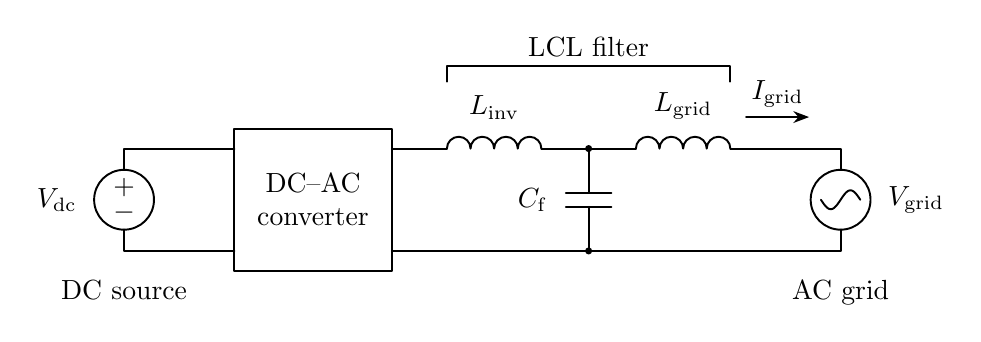
\begin{tikzpicture}[x=1cm,y=1cm,line cap=round,line join=round,
  every node/.style={font=\normalsize},
  wire/.style={line width=0.7pt},
  >={Stealth[length=2mm]}]
  % ---- DC source ---------------------------------------------------------
  \draw[wire] (0,0) circle (0.38);
  \node at (0,0.16) {$+$};
  \node at (0,-0.16) {$-$};
  \node[left] at (-0.48,0) {$V_{\mathrm{dc}}$};
  \draw[wire] (0,0.38) -- (0,0.65) -- (1.4,0.65);
  \draw[wire] (0,-0.38) -- (0,-0.65) -- (1.4,-0.65);
  \node[below] at (0,-0.9) {DC source};
  % ---- converter ---------------------------------------------------------
  \draw[wire] (1.4,-0.9) rectangle (3.4,0.9);
  \node[align=center] at (2.4,0) {DC--AC\\converter};
  % ---- LCL filter on the top rail, return on the bottom rail --------------
  \draw[wire] (3.4,0.65) -- (4.1,0.65);
  \draw[wire] (4.1,0.65)
    arc[start angle=180,end angle=0,radius=0.15]
    arc[start angle=180,end angle=0,radius=0.15]
    arc[start angle=180,end angle=0,radius=0.15]
    arc[start angle=180,end angle=0,radius=0.15];
  \node[above] at (4.7,0.9) {$L_{\mathrm{inv}}$};
  \draw[wire] (5.3,0.65) -- (6.5,0.65);
  \fill (5.9,0.65) circle (0.045);
  \fill (5.9,-0.65) circle (0.045);
  \draw[wire] (5.9,0.65) -- (5.9,0.09);
  \draw[wire] (5.61,0.09) -- (6.19,0.09);
  \draw[wire] (5.61,-0.09) -- (6.19,-0.09);
  \draw[wire] (5.9,-0.09) -- (5.9,-0.65);
  \node[left] at (5.5,0) {$C_{\mathrm{f}}$};
  \draw[wire] (6.5,0.65)
    arc[start angle=180,end angle=0,radius=0.15]
    arc[start angle=180,end angle=0,radius=0.15]
    arc[start angle=180,end angle=0,radius=0.15]
    arc[start angle=180,end angle=0,radius=0.15];
  \node[above] at (7.1,0.9) {$L_{\mathrm{grid}}$};
  \draw[wire] (7.7,0.65) -- (9.1,0.65) -- (9.1,0.38);
  \draw[wire] (3.4,-0.65) -- (9.1,-0.65) -- (9.1,-0.38);
  % ---- AC grid -----------------------------------------------------------
  \draw[wire] (9.1,0) circle (0.38);
  \draw[wire] plot[domain=-0.25:0.25,samples=40,smooth]
    ({9.1+\x},{0.12*sin(deg(\x*3.1416/0.25))});
  \node[right] at (9.58,0) {$V_{\mathrm{grid}}$};
  \node[below] at (9.1,-0.9) {AC grid};
  \draw[wire,->] (7.9,1.05) -- (8.7,1.05);
  \node[above] at (8.3,1.05) {$I_{\mathrm{grid}}$};
  % ---- LCL bracket ---------------------------------------------------------
  \draw[wire] (4.1,1.5) -- (4.1,1.7) -- (7.7,1.7) -- (7.7,1.5);
  \node[above] at (5.9,1.7) {LCL filter};
\end{tikzpicture}

\caption{Three-phase inverter interface, shown as a single-phase equivalent: DC source, converter stage, LCL filter, and AC grid.}
\label{fig:invsymbol}
\end{figure}

The Universal Interoperability for Grid-Forming Inverters (UNIFI) Consortium defines GFM behavior through an internal voltage phasor that remains approximately stiff on subtransient-to-transient timescales \cite{unifi2026}. This characteristic supports an immediate electrical response to changes at the connection point, subject to resource and control limits. It does not mean that voltage magnitude or phase remains fixed indefinitely, or that the inverter behaves as an unlimited voltage source during a severe fault. GFM control takes several forms, including droop and virtual-synchronous-machine implementations \cite{unifi2026,du2023a1,du2024b1}; all maintain that internal voltage phasor as the voltage and frequency reference, and the system-level behavior then depends on the remaining controls, hardware, and operating limits.

ERCOT's Nodal Operating Guide Revision Request (NOGRR) 272 establishes advanced grid-support requirements for inverter-based energy storage resources connected to the ERCOT Transmission Grid \cite{nogrr272}. The applicability trigger is a Standard Generation Interconnection Agreement (SGIA) executed on or after April~1, 2026, rather than the date on which any new battery begins operating. The revision was approved on November~6, 2025, with an effective date of December~1, 2025; the SGIA cutoff is a distinct date \cite{nogrr272,agsupdate2026}. This distinction matters when describing the population of resources to which the requirements apply.

\begin{figure}[tbp]\centering
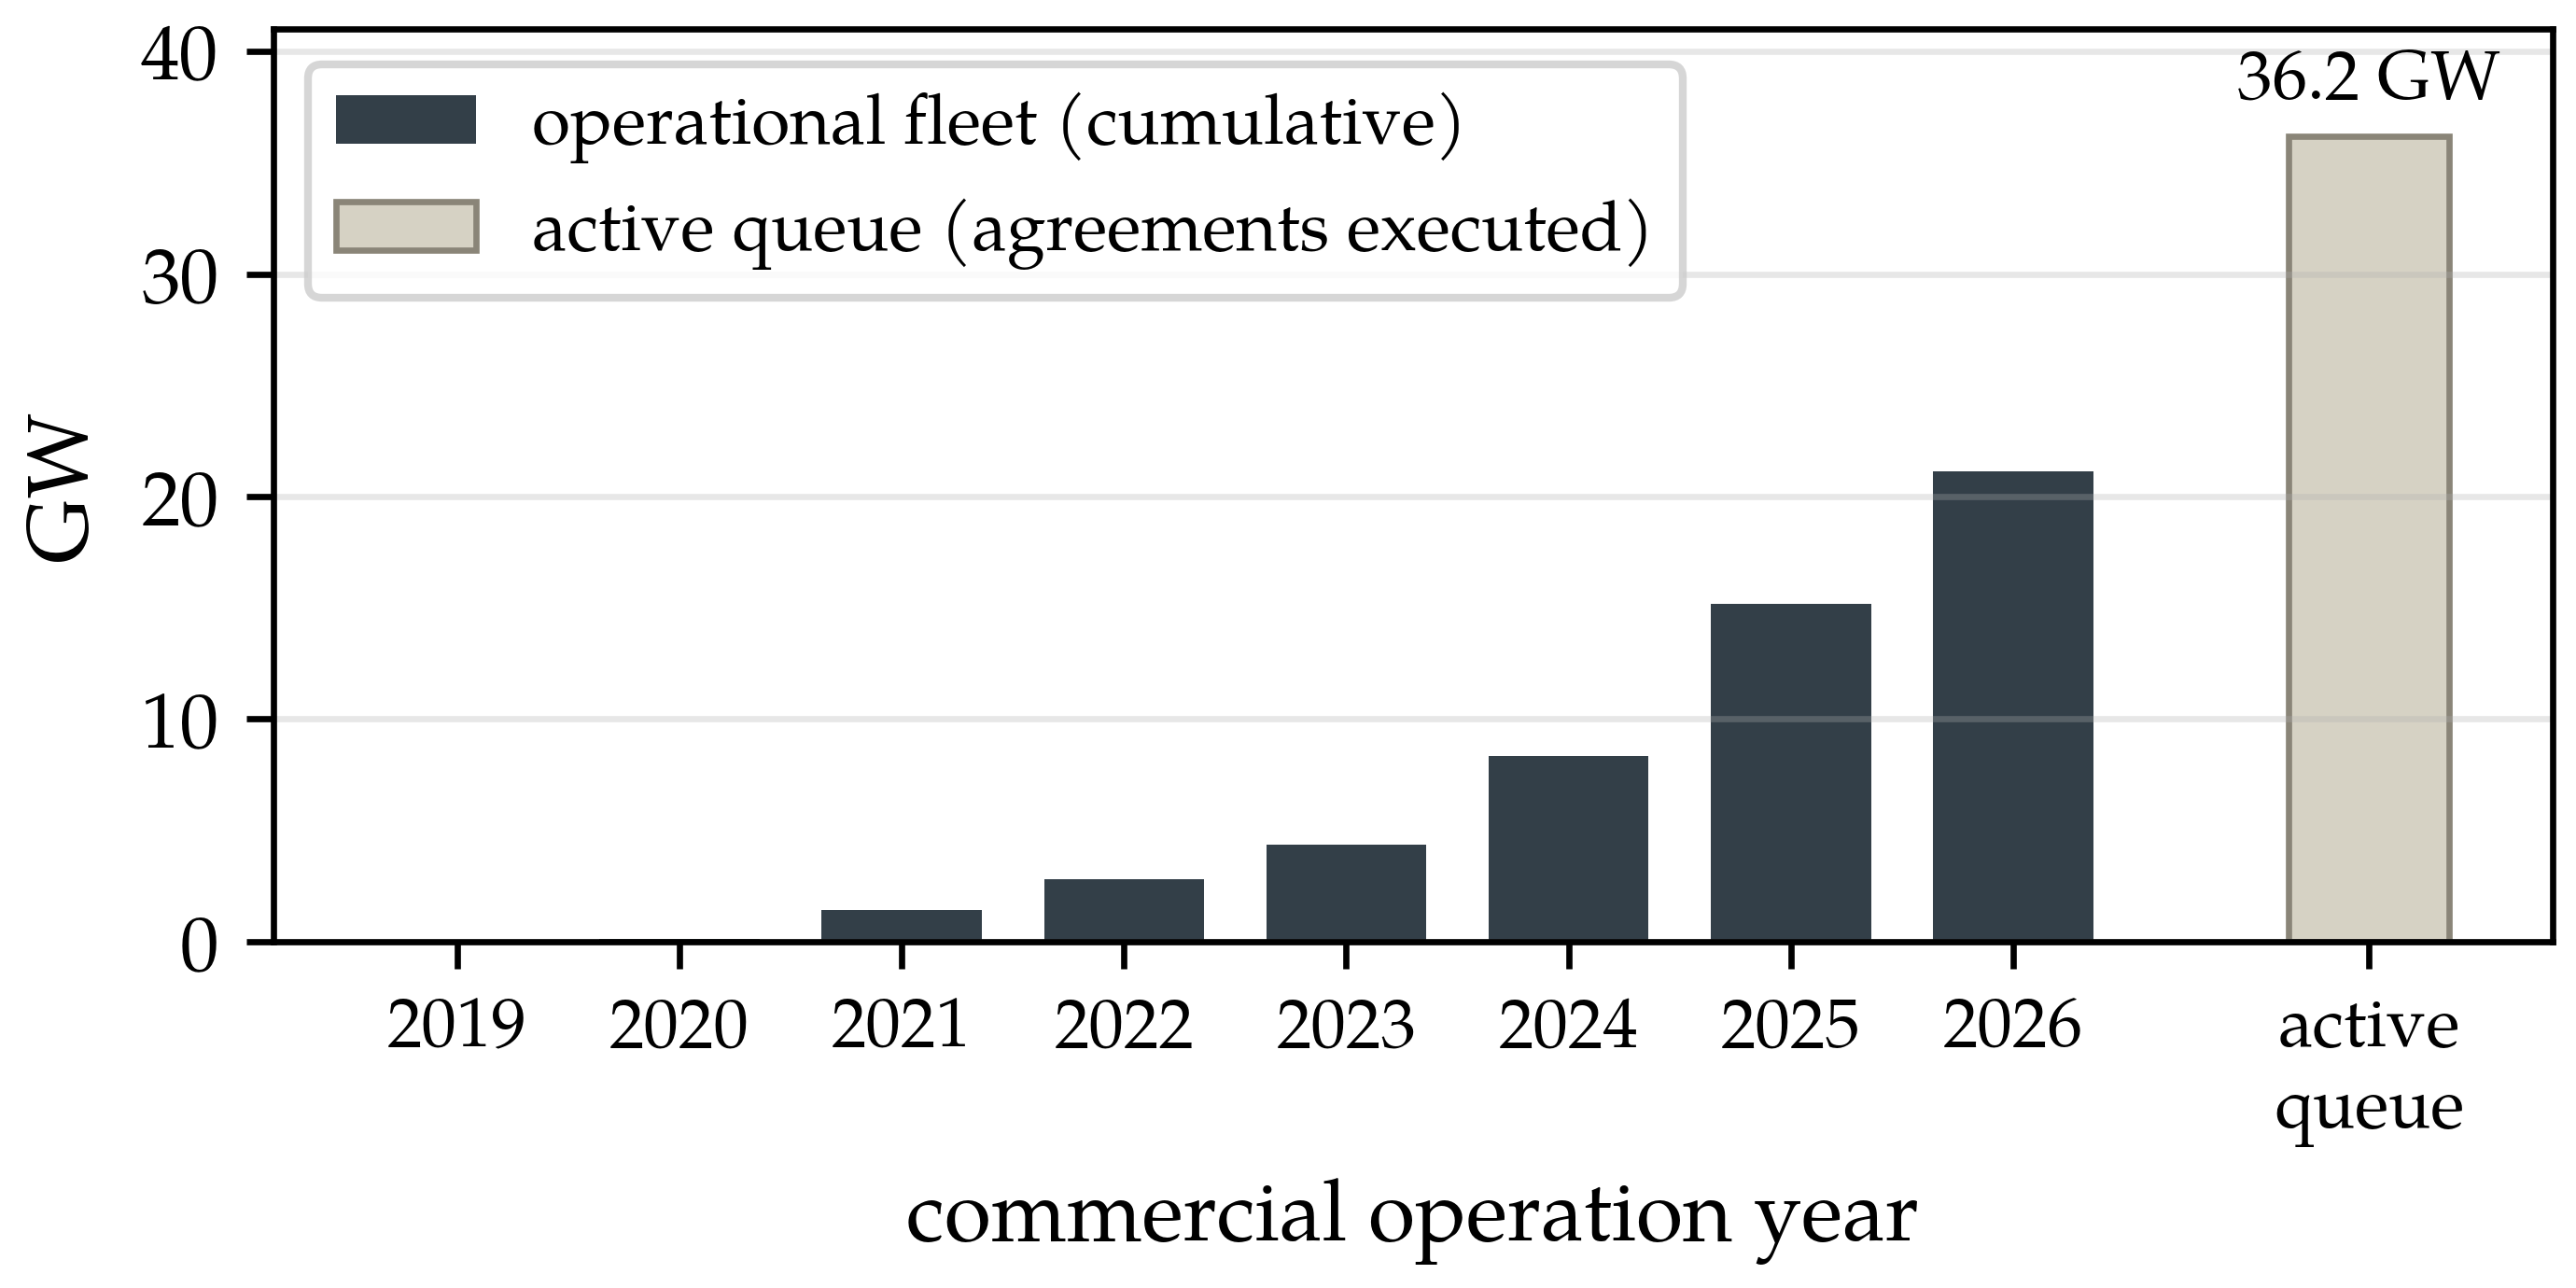
\includegraphics[width=0.708\textwidth]{bess_fleet_growth}
\caption{ERCOT battery energy storage capacity by commercial-operation year, alongside 36.2~GW in the interconnection queue with executed agreements \cite{mora2026,gis2026}.}
\label{fig:ercotbess}
\end{figure}

\label{sec:gflgfm}

Conventional grid-following (GFL) control uses an externally established voltage waveform as its synchronization reference, commonly through a phase-locked loop. Within normal voltage limits, a GFL's output current phasor remains unchanged immediately after a disturbance, before outer controls adjust the injected power \cite{unifi2026}.  The GFM versus GFL distinction concerns control behavior and synchronization.

Three terms connect GFM controls to the machine-based interpretation developed in this report. Mathematical equation of the GFM and synchronous machine dynamics does not reflect a physical equation of inverter-based resources with synchronous generators.
\begin{enumerate}
\item The \emph{inverter angle} is a controller-generated electrical phase angle. Like a machine's electrical rotor angle, its displacement relative to other sources influences power transfer. Inverter angle is not the position of a physical shaft or rotor winding.
\item The \emph{equivalent inertia} of filtered droop arises from the temporal lag associated with filtered-active-power measurement and depends on the active-power-filter time constant and droop gain relating changes in frequency to changes in active power \cite{chatterjee2026note,chatterjee2025eac}. A longer filter time constant or a smaller droop gain raises this equivalent inertia coefficient, and with it the inverter angle's resistance to acceleration. 
\item The \emph{equivalent damping} relates normalized frequency deviation to normalized power response. The droop gain sets this coefficient in the reduced GFM model.
\end{enumerate}
Section~\ref{sec:testbed} describes the network, resource models, and simulation workflow. Section~\ref{sec:emt} presents the EMT replacement and fault-response studies. Section~\ref{sec:dynamics} develops the machine-to-GFM comparison and interprets the inertia estimation tests. Section~\ref{sec:outlook} presents the preliminary energy analysis and next-phase directions.

\section{Simulation Testbed}
\label{sec:testbed}
The testbed provides a configurable network for the machine-to-inverter comparison. We converted the PSS/E case to PSCAD with E-TRAN and used the EMT representation for the first-year disturbance studies. This construction also preserves a common starting point for future corresponding-model comparisons.

\subsection{Testbed Construction}
The adapted IEEE 39-bus network contains ten generator buses \cite{pscad39bus,pscad39note}. Its EMT representation includes Bergeron transmission lines, generator step-up transformers, and constant-power loads (E-TRAN load model type~0: fixed real and reactive power) \cite{pscadbergeron}. E-TRAN translates the network parameters and initial load-flow operating point from PSS/E into PSCAD \cite{etran}. The resulting benchmark uses a 230~kV transmission network with representative ERCOT-supplied machine dynamics.

The ten synchronous machine models share GENROU, ESST4B, GGOV1, and PSS2B dynamic parameters, including inertia $H=5.46$~s. Sharing these parameters does not imply identical ratings or dispatch. Figure~\ref{fig:testbedflow} summarizes the construction and processing workflow. Figures~\ref{fig:faultlogic} and~\ref{fig:faultcontrol} show the controls used to select fault location, type, timing, and associated breaker action.

The fault controls combine a central configuration panel with logic attached to individual transmission lines. We specify the fault start time, location, type (e.g. single line, double line, or all three lines to ground fault), and duration, while the line controls implement the corresponding fault and breaker commands. The protection settings distinguish removal of the fault from restoration of the connection. This arrangement allows the same network to support either a reclosed connection or a post-fault topology in which the selected connection remains open.

\begin{figure}[tbp]\centering
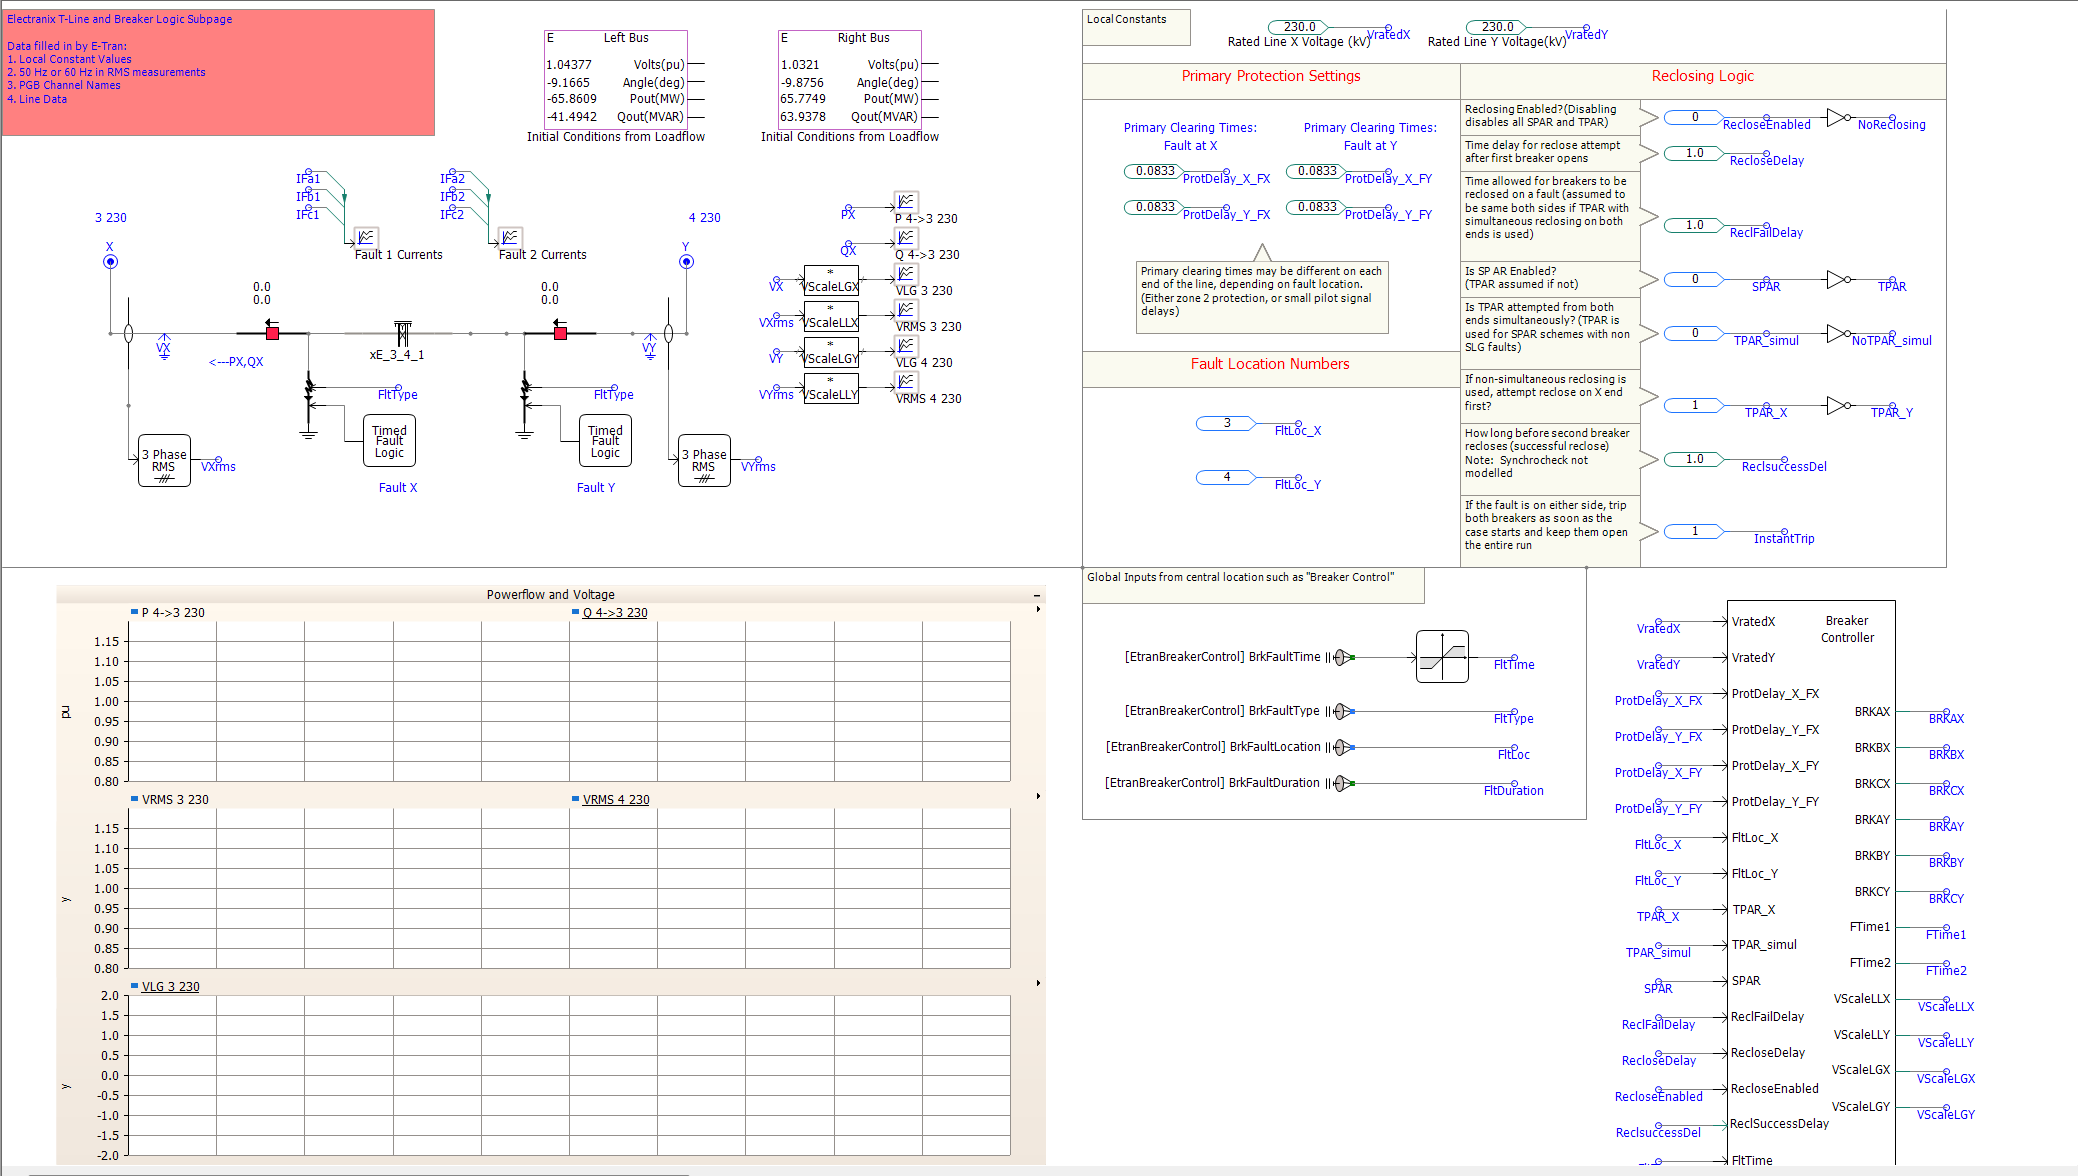
\includegraphics[width=\textwidth]{pscad_fault_line_logic}
\caption{Fault and protection configuration on one E-TRAN-converted
line, as presented in the PSCAD user interface: the per-line timed
fault logic and measurement channels (left), and the primary
protection clearing times, reclosing logic, fault-location numbers,
and breaker controller (right). }
\label{fig:faultlogic}
\end{figure}

\begin{figure}[tbp]\centering
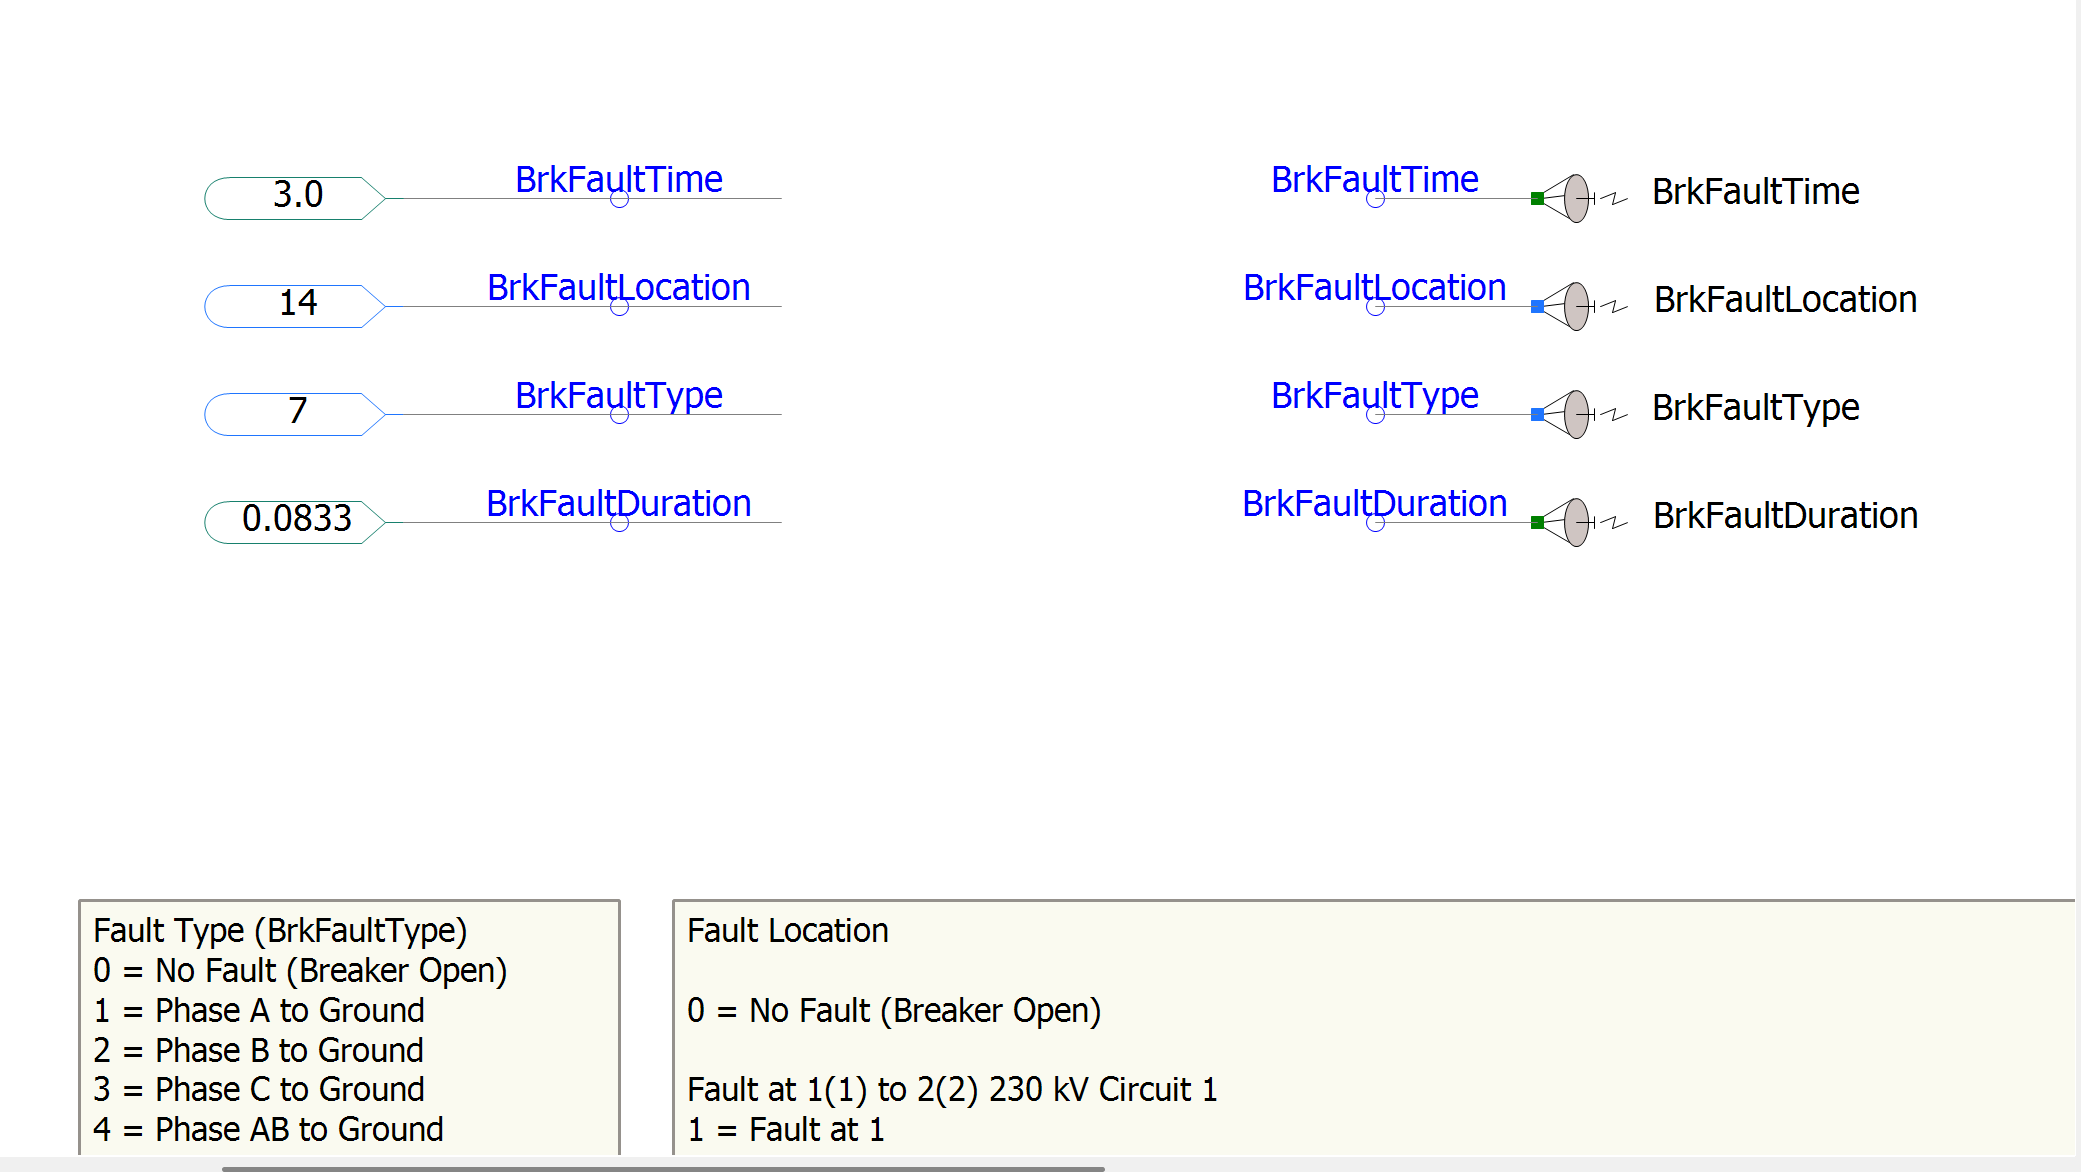
\includegraphics[width=0.9\textwidth]{pscad_breaker_fault_control}
\caption{Central fault-control settings for the bus-14 reference disturbance: start time 3.0~s, type code 7 (3 phase to ground fault), and duration 0.0833~s, approximately five cycles at 60~Hz.}
\label{fig:faultcontrol}
\end{figure}

\subsection{Iterative Generator Replacement}
One design goal was to study mixtures of synchronous machines and GFM inverters in the same network. Each generator location can retain its machine or host an inverter, with the operating point specified in that resource's PSCAD model. We configured the replacements manually for the first study; the PSCAD Python interface (\texttt{mhi.pscad}) also provides a path to automated configuration.

We developed eleven configurations by replacing zero through ten machines with GFM units. Because generator ratings and operating points are not identical, replacement count identifies the cases without assuming that each replacement corresponds to exactly 10\% of generation capacity. The progression spans the all-machine and all-GFM endpoints while retaining a common reference disturbance. The framework can also accommodate alternative GFM models, machine dynamics, and GFL resources for later mixed-system studies.

\subsection{Measurement in Testbed Design}
The instrumentation records per-bus instantaneous and root-mean-square (RMS) voltage and current, active and reactive powers, and frequency quantities in addition to instantaneous line to neutral voltage and line to line current. We parse the PSCAD (.out) output files and normalize device quantities on their apparent-power bases for plotting.

Voltage and current interpretation depends on the selected bases and on whether the signal is instantaneous or RMS. We distinguish line-to-line voltage from line-to-neutral voltage when interpreting the three-phase quantities.  Appendix~\ref{app:plotting} describes the channel-processing conventions.

\begin{figure}[tbp]\centering
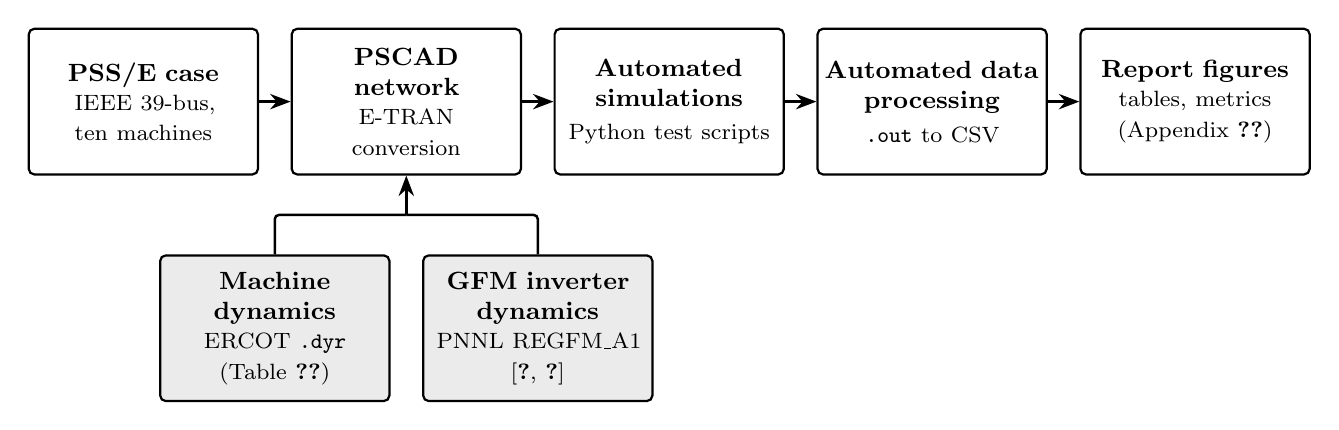
\begin{tikzpicture}[
  font=\small,
  box/.style={draw=black, line width=0.8pt, rounded corners=2pt, align=center,
              inner sep=3pt, text width=27mm, minimum height=18.5mm, fill=white},
  input/.style={box, fill=black!8},
  wire/.style={line width=0.9pt, color=black, rounded corners=1.5pt},
  arr/.style={wire, -{Stealth[length=2.6mm]}}
]
\node[box] (psse) {\textbf{PSS/E case}\\[1pt]
  {\footnotesize IEEE 39-bus,\\ten machines}};
\node[box, right=4mm of psse] (pscad) {\textbf{PSCAD network}\\[1pt]
  {\footnotesize E-TRAN\\conversion}};
\node[box, right=4mm of pscad] (run) {\textbf{Automated\\simulations}\\[1pt]
  {\footnotesize Python test scripts}};
\node[box, right=4mm of run] (proc) {\textbf{Automated data\\processing}\\[1pt]
  {\footnotesize \texttt{.out} to CSV}};
\node[box, right=4mm of proc] (figs) {\textbf{Report figures}\\[1pt]
  {\footnotesize tables, metrics\\(Appendix~\ref{app:plotting})}};
\node[input, below=10mm of pscad, xshift=-16.7mm] (sm)
  {\textbf{Machine\\dynamics}\\[1pt]
  {\footnotesize ERCOT \texttt{.dyr}\\(Table~\ref{tab:dyr_gov_params})}};
\node[input, below=10mm of pscad, xshift=16.7mm] (gfm)
  {\textbf{GFM inverter\\dynamics}\\[1pt]
  {\footnotesize PNNL REGFM\_A1\\\cite{du2023a1,pnnlgithub}}};
\draw[arr] (psse) -- (pscad);
\draw[arr] (pscad) -- (run);
\draw[arr] (run) -- (proc);
\draw[arr] (proc) -- (figs);
\coordinate (j) at ([yshift=-5mm]pscad.south);
\draw[wire] (sm.north) |- (j);
\draw[wire] (gfm.north) |- (j);
\draw[arr] (j) -- (pscad.south);
\end{tikzpicture}
\caption{Testbed workflow: E-TRAN converts the IEEE 39-bus PSS/E case into a PSCAD EMT network; the ERCOT-supplied synchronous-machine dynamics and the PNNL REGFM\_A1 grid-forming inverter dynamics are inserted into that network; Python scripts set up and run the simulations and convert the EMTDC output into tables, metrics, and the report's figures. The interpretation of those results is not automated.}
\label{fig:testbedflow}
\end{figure}

Table~\ref{tab:dyr_gov_params} lists the governor and turbine settings used by the machine model. Appendix~\ref{app:params} gives the machine, excitation, governor, and stabilizer record in PSS/E format. These dynamic settings act alongside the network operating point to determine the machine response. The parameter units follow the corresponding normalized control signals \cite{pestr1,pssemodels}.

The machine model includes the rotor and field dynamics, an exciter, a turbine governor, and a power-system stabilizer. The GGOV1 settings specify permanent droop, the speed-error limits, valve motion, turbine response, and load and acceleration limits. The transducer time $T_{\mathrm{pelec}}=1.0$~s filters the electrical-power feedback selected by Rselect~$=1$; it is the supplied value, equal to the typical GGOV1 value tabulated in \cite{pestr1}, and is distinct from the inverter's 10~ms power-measurement filter and from any plotting filter. 

\begin{table}[tbp]\centering\small
\caption{GGOV1 governor and turbine parameters for the synchronous-machine reference, in the order of the PSS/E GGOV1 record \cite{pssemodels}; typical values and the block diagram are in \cite{pestr1}.}
\label{tab:dyr_gov_params}
\begin{tabular}{>{\raggedright\arraybackslash}p{0.23\linewidth}>{\raggedright\arraybackslash}p{0.13\linewidth}>{\raggedright\arraybackslash}p{0.17\linewidth}>{\raggedright\arraybackslash}p{0.34\linewidth}}\toprule
Parameter & Value & Units & Definition\\\midrule
Rselect (ICON) & 1 & integer & Electrical-power droop feedback\\
Flag (ICON) & 1 & switch & Fuel-flow characteristic\\
$R$ & 0.05 & p.u./p.u. & Permanent droop\\
$T_{\mathrm{pelec}}$ & 1.0 & s & Electrical-power transducer time\\
maxerr / minerr & $\pm0.055$ & p.u. & Governor speed-error clip (PID input)\\
$K_{\mathrm{pgov}}$ & 10 & p.u./p.u. & Proportional gain\\
$K_{\mathrm{igov}}$ & 1 & s$^{-1}$ & Integral gain\\
$K_{\mathrm{dgov}}$ & 0 & s & Derivative gain\\
$T_{\mathrm{dgov}}$ & 1 & s & Derivative-filter time\\
$v_{\mathrm{max}} / v_{\mathrm{min}}$ & 1 / 0.16 & p.u. & Valve-position limits\\
$T_{\mathrm{act}}$ & 0.5 & s & Actuator time constant\\
$K_{\mathrm{turb}}$ & 1.5 & p.u./p.u. & Turbine gain\\
$W_{\mathrm{fnl}}$ & 0.2 & p.u. & No-load fuel flow\\
$T_{\mathrm{b}}$ & 0.1 & s & Turbine lag time\\
$T_{\mathrm{c}}$ & 0 & s & Turbine lead time\\
$T_{\mathrm{eng}}$ & 0 & s & Engine transport lag\\
$T_{\mathrm{fload}}$ & 3 & s & Load-limiter time constant\\
$K_{\mathrm{pload}} / K_{\mathrm{iload}}$ & 2 / 0.7 & p.u./p.u. / s$^{-1}$ & Load-limiter PI gains\\
$L_{\mathrm{dref}}$ & 1 & p.u. & Load-limiter reference\\
$D_{\mathrm{m}}$ & 0 & p.u./p.u. & Turbine speed sensitivity\\
$R_{\mathrm{open}} / R_{\mathrm{close}}$ & $0.1/-0.1$ & p.u./s & Valve motion limits\\
$K_{\mathrm{imw}}$ & 0 & s$^{-1}$ & Power-controller reset gain; disabled\\
$A_{\mathrm{set}}$ & 0.1 & p.u./s & Acceleration setpoint\\
$K_{\mathrm{a}} / T_{\mathrm{a}}$ & 10 / 0.1 & p.u. / s & Acceleration gain/filter time\\
$T_{\mathrm{rate}}$ & 0 & MW & Turbine-rating input\\
db & 0.0002 & p.u. & Speed-governor deadband\\
$T_{\mathrm{sa}} / T_{\mathrm{sb}}$ & 4 / 5 & s / s & Temperature lead/lag times\\
$R_{\mathrm{up}} / R_{\mathrm{down}}$ & $99/-99$ & p.u./s & Load-limit ramp caps; inactive\\\bottomrule
\end{tabular}
\end{table}

\begin{figure}[tbp]\centering
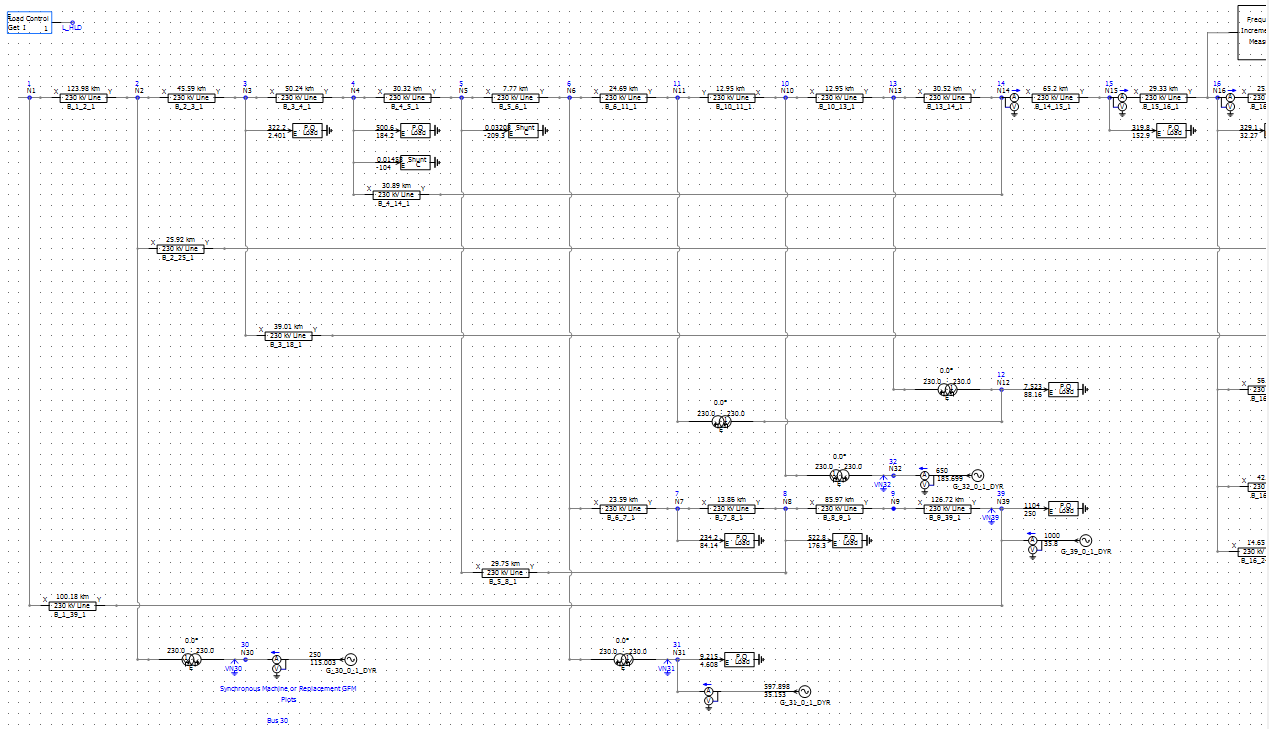
\includegraphics[width=0.93\textwidth]{pscad_39bus_overview}
\caption{Single-line overview of the E-TRAN-converted IEEE
39-bus network on the PSCAD canvas: 230~kV lines with per-line length
labels, transformers, and the ten generator subsystems.}
\label{fig:pscad39}
\end{figure}

\begin{figure}[tbp]\centering
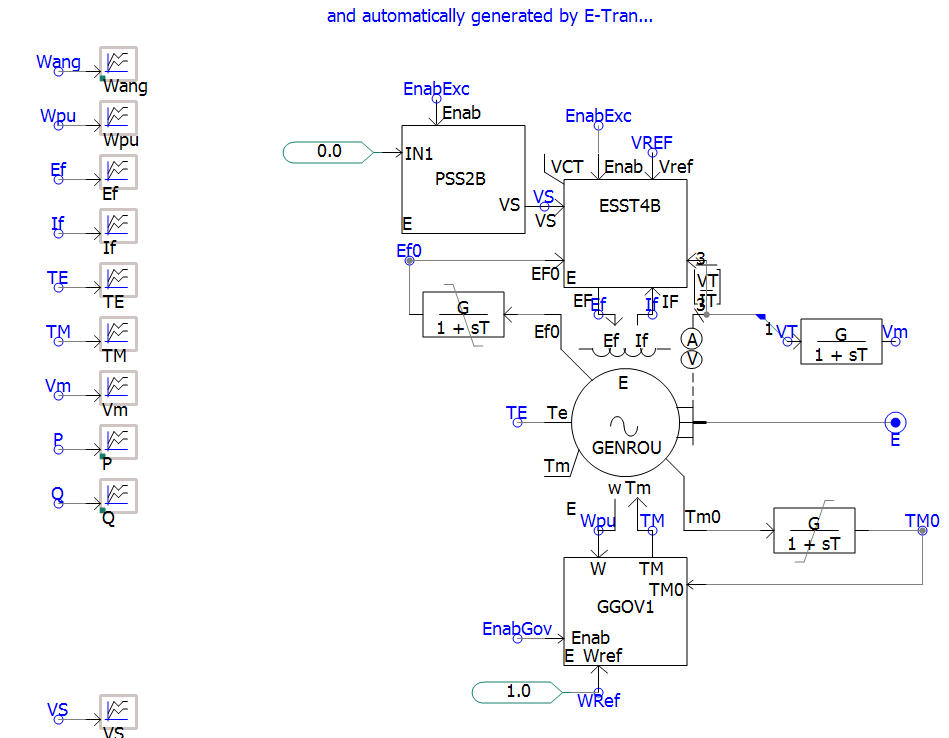
\includegraphics[width=0.66\textwidth]{pscad_machine_internals}
\caption{Machine subsystem internals as generated by E-TRAN
from the \texttt{.dyr} record: the GENROU machine with its PSS2B
stabilizer, ESST4B exciter, and GGOV1 governor blocks, plus the
per-signal recorder taps.}
\label{fig:pscadmachine}
\end{figure}

\subsection{GFM Inverter Models Evaluated in Simulation Testbed}
We use the Pacific Northwest National Laboratory (PNNL) REGFM\_A1 droop-controlled model in the 39-bus system studies \cite{du2023a1}. REGFM\_A1 is an average-voltage source model. PNNL also developed switching-level models, but those models often those run too slow to be useful for practical power systems studies. In addition, we tested REGFM\_B1 from PNNL. REGFM\_B1 is a virtual synchronous machine model (VSM) and was evaluated in model-quality and inertia tests \cite{du2024b1}. PNNL provides these models for PSCAD and PSS/E \cite{pnnlgithub}. The REGFM\_A1 single-device tests include low-voltage ride-through, voltage and phase-angle steps, and frequency disturbances; Figure~\ref{fig:smibgfm} shows its fault response.

For each replacement, we use the sizing rule $S_{\mathrm{inv,base}}=P_{\mathrm{G}}/0.6$, where $P_{\mathrm{G}}$ is the replaced machine's MW dispatch and $S_{\mathrm{inv,base}}$ is expressed in MVA. The selected inverter active-power reference is 0.6 per unit on that base, the PSCAD component's default, as published by PNNL (Figure~\ref{fig:pscada1params}). Matching the replaced MW at that reference fixes the base, whereas keeping the machine rating as the base would have required changing the reference, which was not done in the first-year runs. The rule preserves the intended MW injection but does not necessarily preserve the original machine's MVA rating or headroom. The inverter connects behind the step-up transformer at the replaced generator location.

\begin{figure}[tbp]\centering
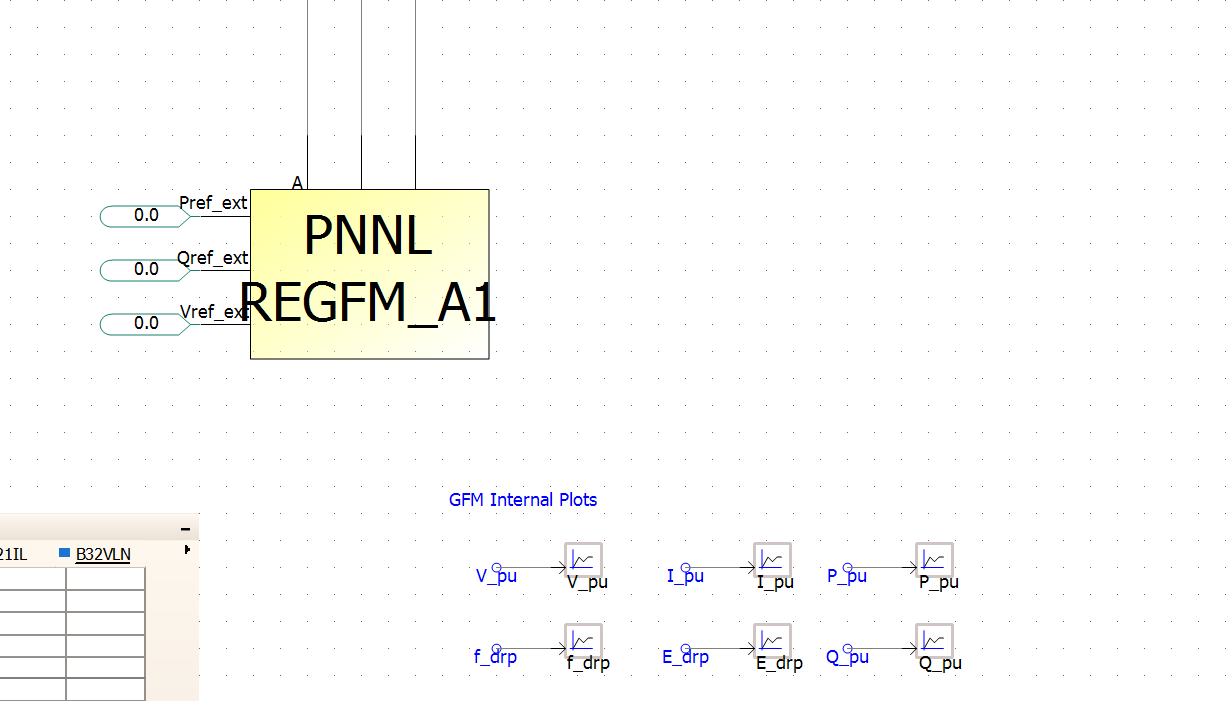
\includegraphics[width=0.85\textwidth]{pscad_regfma1_closeup}
\caption{The PNNL REGFM\_A1 component wired at a replaced
machine bus, behind its 230/10~kV step-up transformer, with the
external reference inputs and the internal-signal plotting modules.}
\label{fig:pscada1closeup}
\end{figure}

\subsection{Model Quality Testing}
\label{sec:mqt}
Model quality testing (MQT) applies the perturbations of the ERCOT Dynamics Working Group procedure manual \cite{dwg24} to prospective inverter and machine models before interpreting their network responses. We used PMView, versions 2.4 and 3.5, as the playback and measurement harness \cite{pmview}. PMView replaces the grid source with a programmable infinite-bus voltage source and applies the test profiles described by the Dynamics Working Group Procedure Manual, Revision~24 \cite{dwg24}. The tests characterize initialization, voltage regulation, ride-through, and response to angle changes.

Tests 1--9 include flat start, legacy and IEEE 2800 low- and high-voltage ride-through, small voltage steps, and phase-angle jumps. PMView version 3.5 adds advanced grid-support tests, including the inertia estimation test discussed in Section~\ref{sec:inertiaest}. These device-level responses help distinguish controller behavior from interactions introduced by the network. The following models were included in the test program.
\begin{enumerate}
\item \textbf{PNNL REGFM\_A1}: droop control with voltage regulation, current control, and current limiting \cite{du2023a1}.

\begin{figure}[tbp]\centering
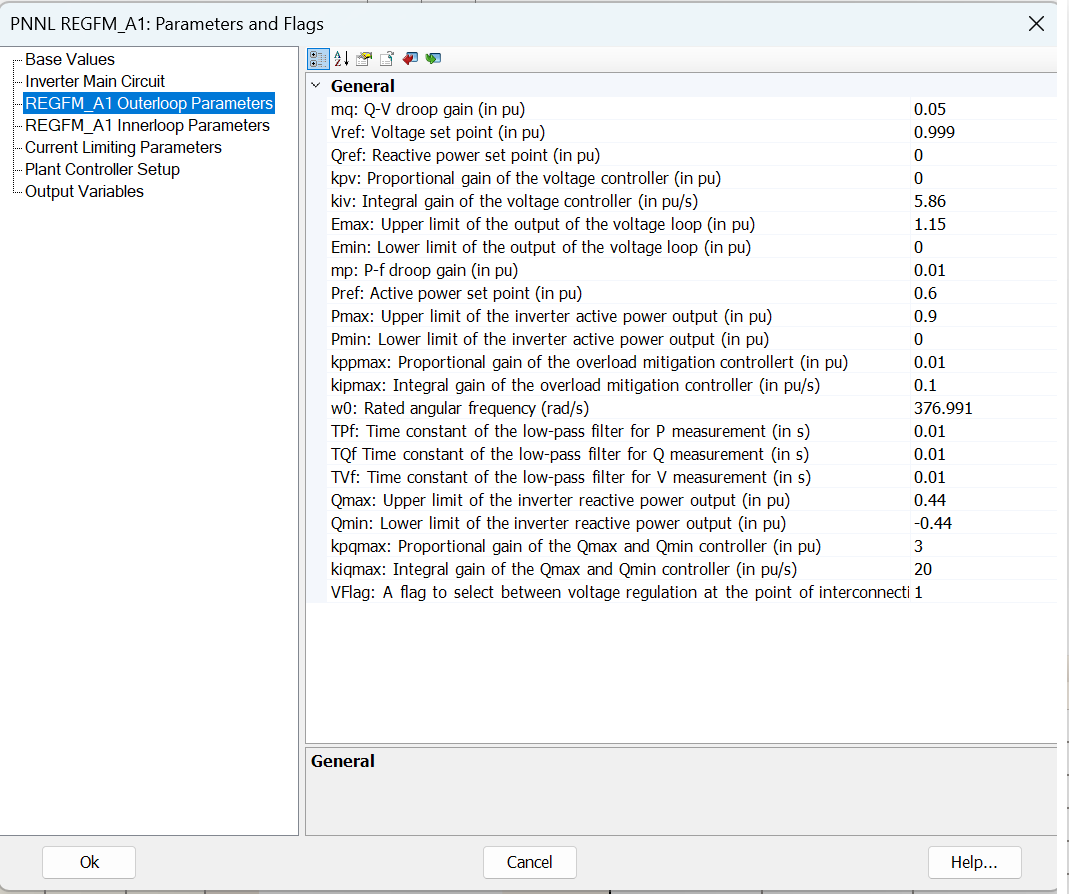
\includegraphics[width=0.68\textwidth]{pscad_regfma1_params}
\caption{REGFM\_A1 outer-loop parameter dialog as configured
for the study: droop gains $m_{\mathrm{p}}=0.01$ and $m_{\mathrm{q}}=0.05$, filter time
constants $T_{\mathrm{Pf}}=T_{\mathrm{Qf}}=10$~ms, and voltage-loop ceiling
$E_{\mathrm{max}}=1.15$~p.u.}
\label{fig:pscada1params}
\end{figure}

\item \textbf{PNNL REGFM\_B1}: a VSM variant evaluated in the model-quality and inertia estimation tests \cite{du2024b1}.

\begin{figure}[tbp]\centering
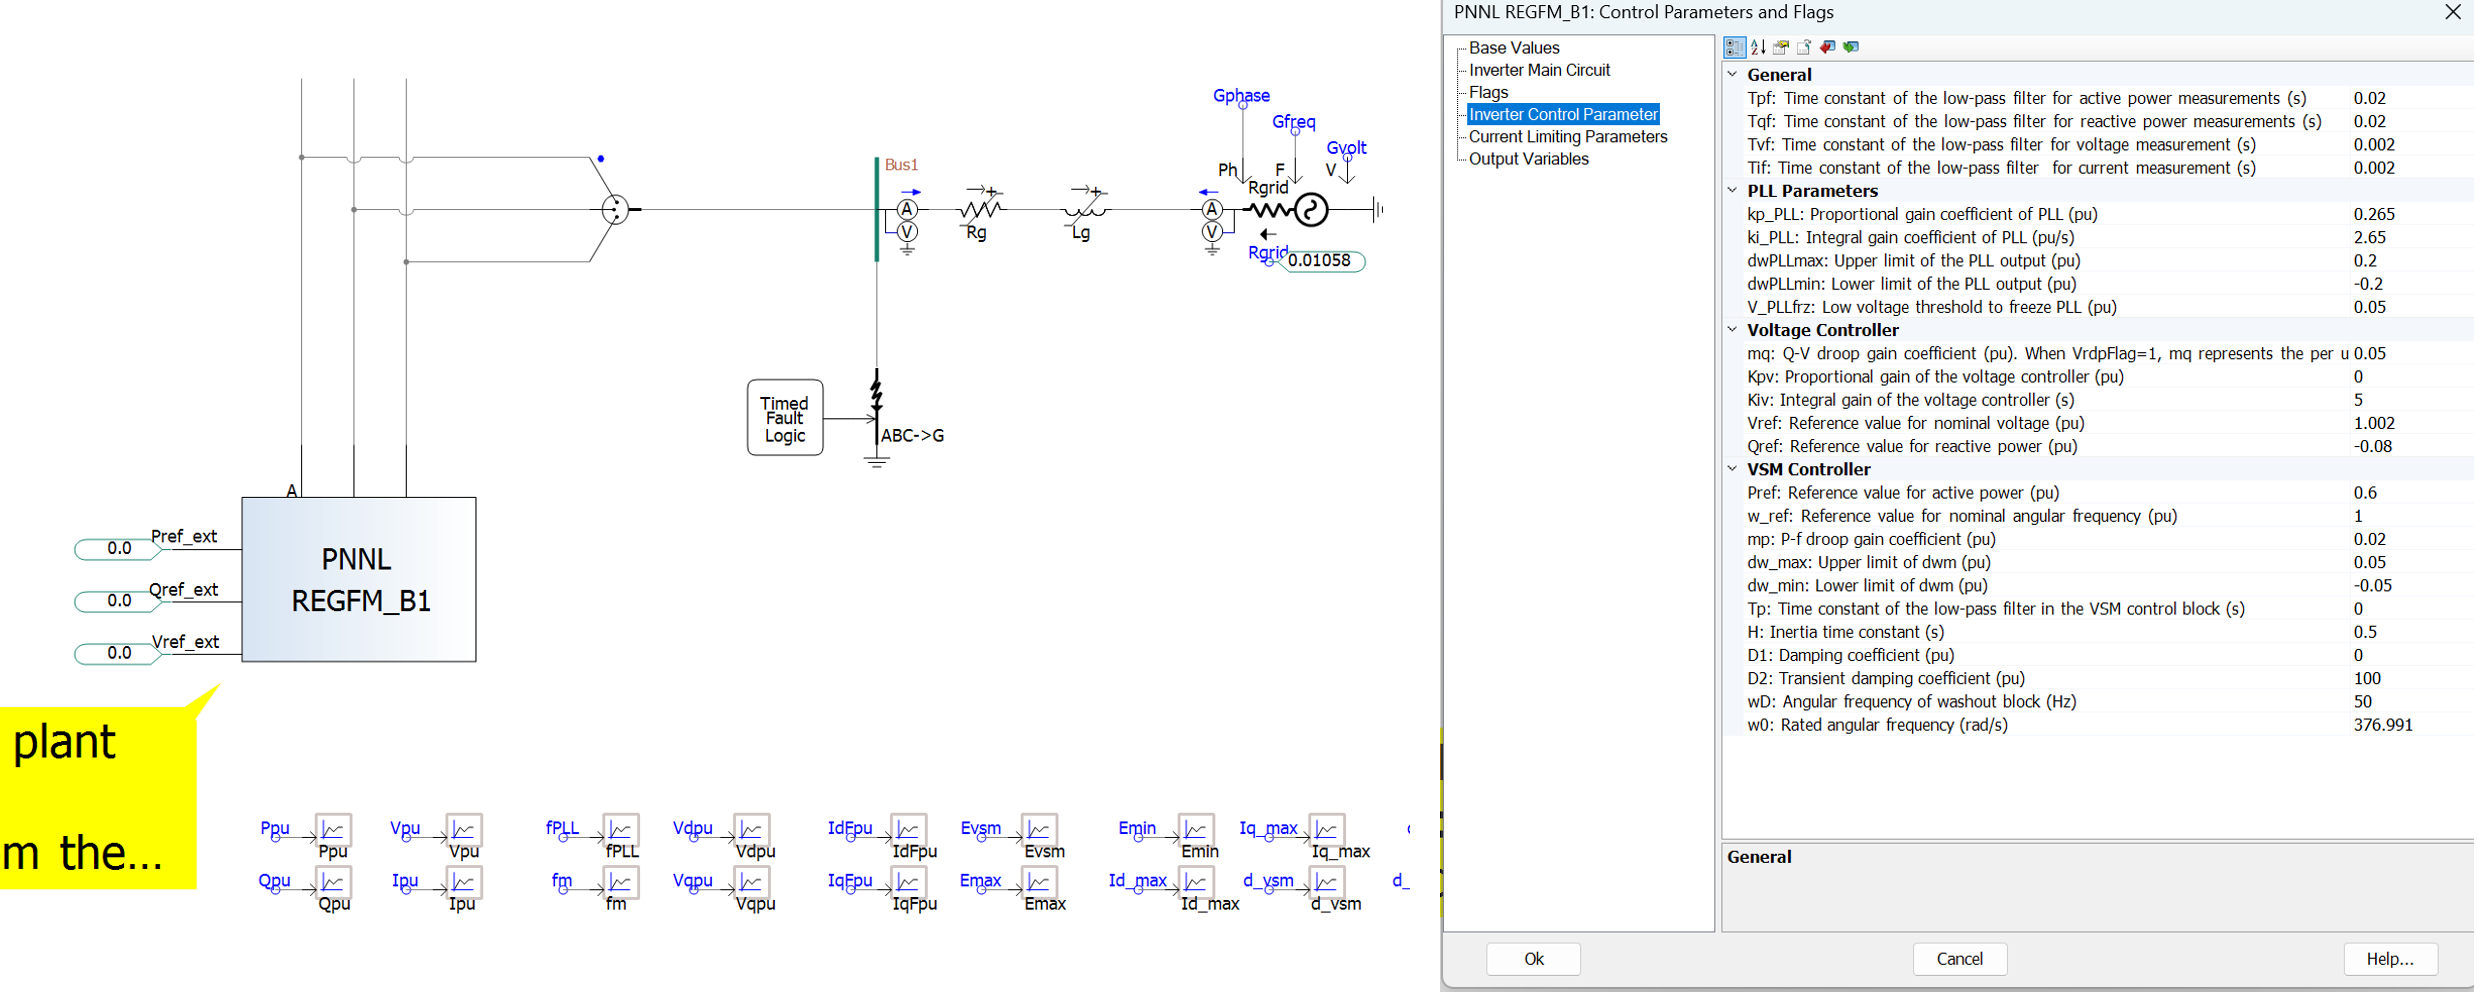
\includegraphics[width=\linewidth]{pscad_regfmb1_block_params}
\caption{REGFM\_B1 in its PMView-driven test harness (left) and
its control-parameter dialog (right); the virtual-synchronous-machine
block carries a configured equivalent inertia constant $H=0.5$~s.}
\label{fig:pscadb1rig}
\end{figure}

\item \textbf{National Laboratory of the Rockies (NLR) GFM model}: droop control with an integral voltage regulator \cite{pypscad}.

\item \textbf{PSCAD library GFM model}: also included in the model-quality-testing program \cite{pscadgfm}.

\begin{figure}[tbp]\centering
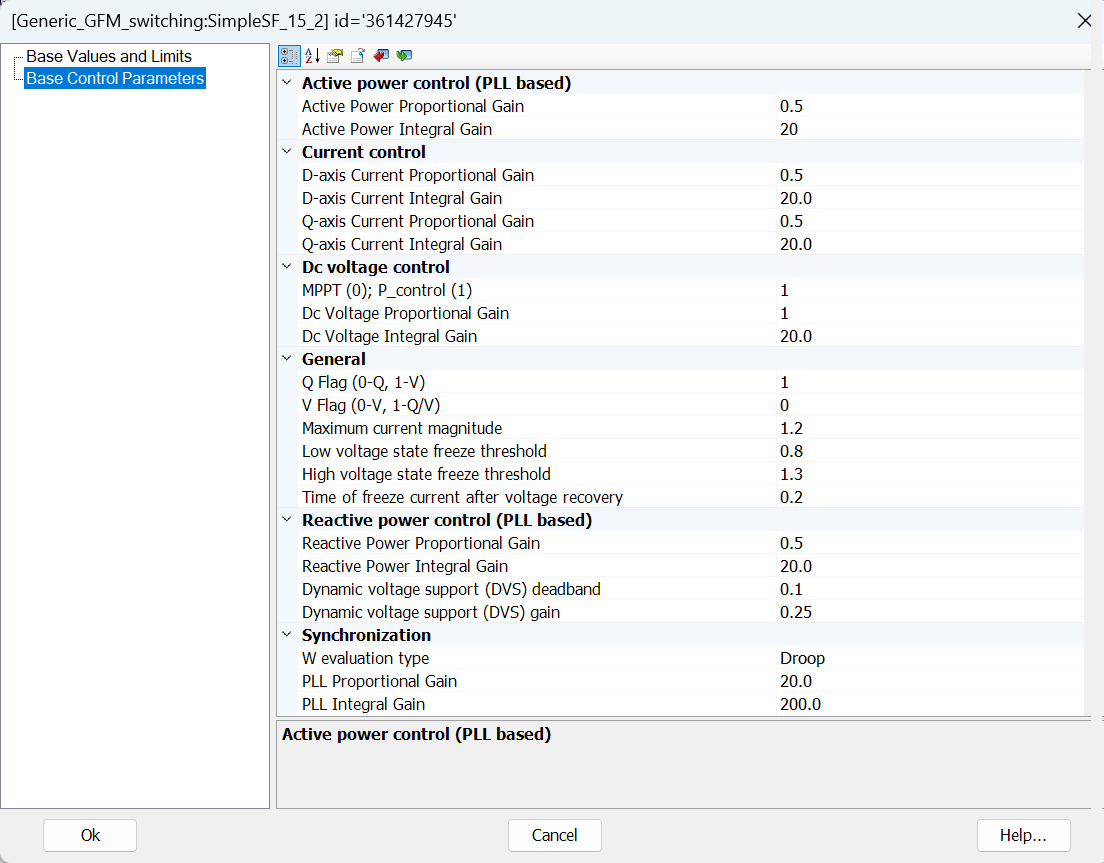
\includegraphics[width=0.68\textwidth]{pscad_generic_gfm_params}
\caption{PSCAD library GFM model:
control-parameter dialog of the aggregated inverter (droop
synchronization, current and voltage loops, and limiter settings).}
\label{fig:pscadgeneric}
\end{figure}

\end{enumerate}

\begin{figure}[tbp]\centering
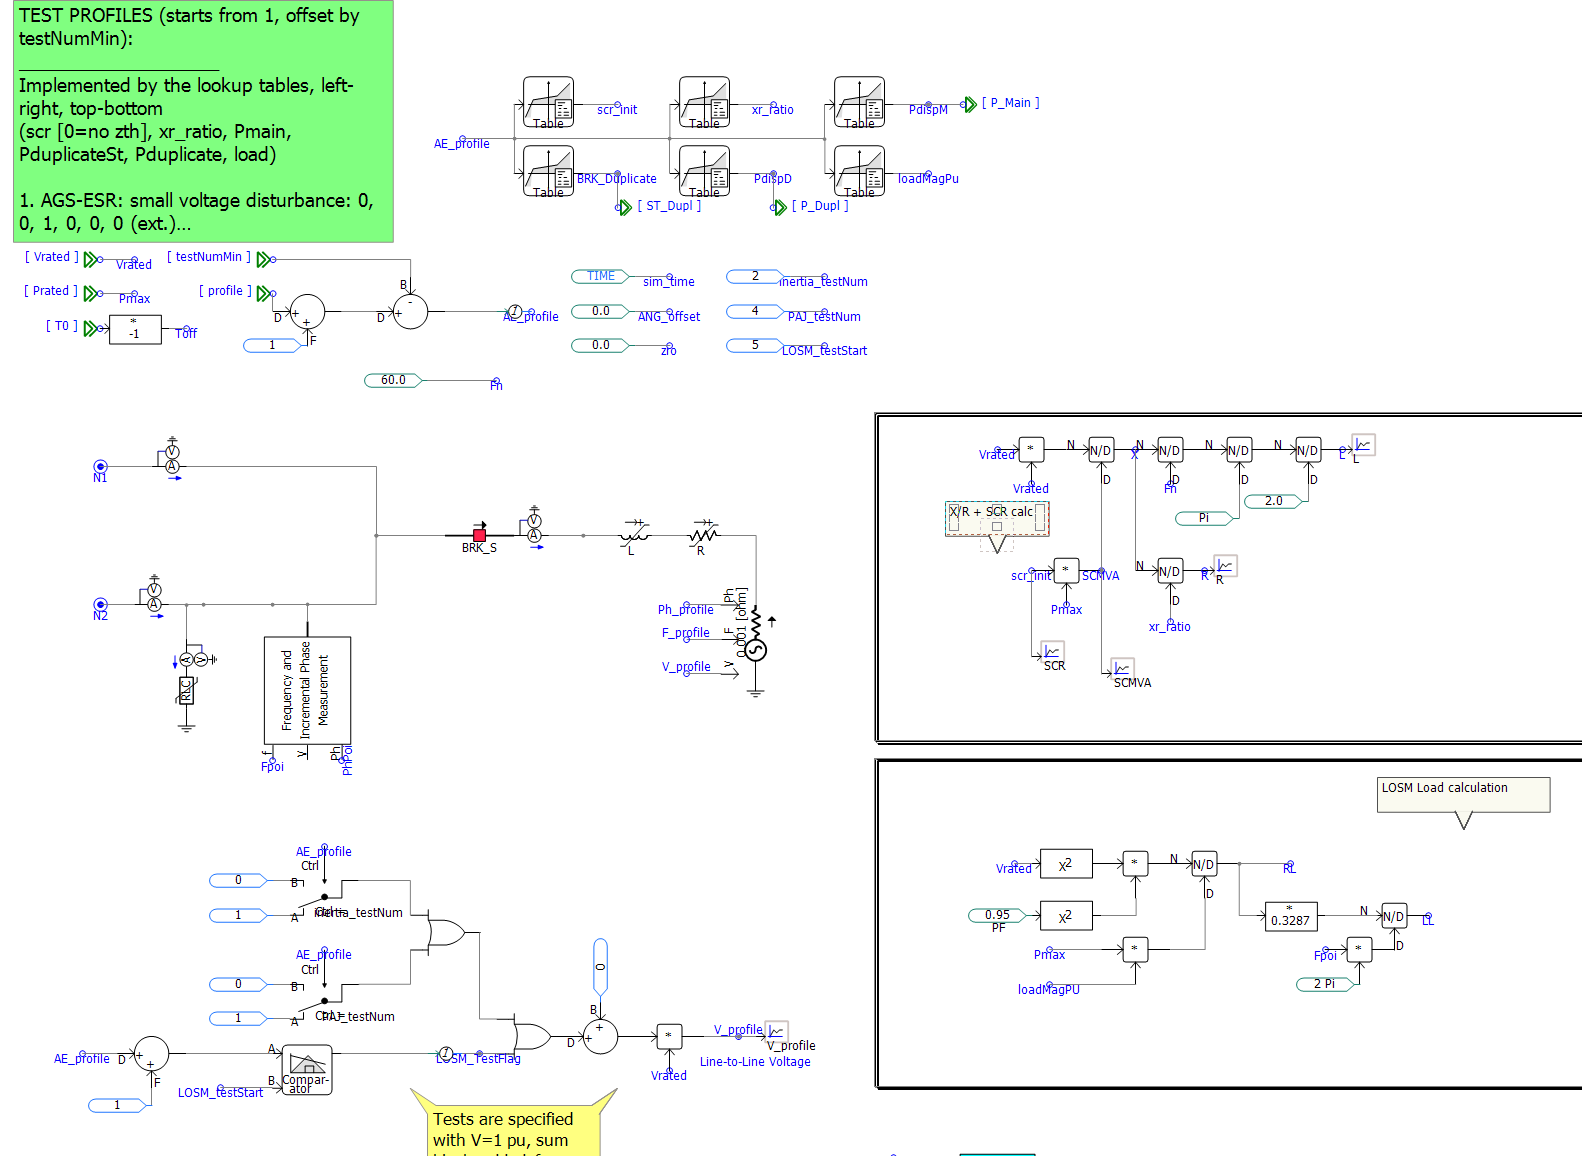
\includegraphics[width=0.85\textwidth]{pscad_pmview_setup}
\caption{PMView test setup: the playback source and
point-of-interconnection measurement wired around the device under
test, with the per-test profile lookup tables that program the
disturbance battery.}
\label{fig:pscadpmview}
\end{figure}

Four models were evaluated: REGFM\_A1, REGFM\_B1, the NLR GFM model, and the PSCAD library GFM model. REGFM\_A1 was selected for the system studies as the most-usable as-shipped model.

We applied the same nine-test battery to the synchronous machine used in the network studies. The machine completed these tests successfully and provides a conventional reference for the inverter comparisons. Figure~\ref{fig:mqtmachine} shows its response to the legacy low-voltage ride-through profile, corresponding to the REGFM\_A1 example in Figure~\ref{fig:mqt}. The machine voltage-step result in Figure~\ref{fig:mqtmachinestep} uses a different step magnitude from the inverter comparison.

The machine example is the 650~MVA Gen-32 test case. Its small-step test raises voltage from 1.00 to 1.03 per unit at 3~s and produces a slower response than the selected REGFM\_A1 comparison. Figure~\ref{fig:smibgfm} shows a separate check outside the PMView profiles: one REGFM\_A1 unit, dispatched at 0.60 per unit against an infinite bus with a short-circuit ratio of 10, rides through a five-cycle bolted three-phase fault at its point of interconnection. Voltage, current, active power, reactive power, and droop frequency together describe how the device supplies the grid through the disturbance.

\begin{figure}[tbp]\centering
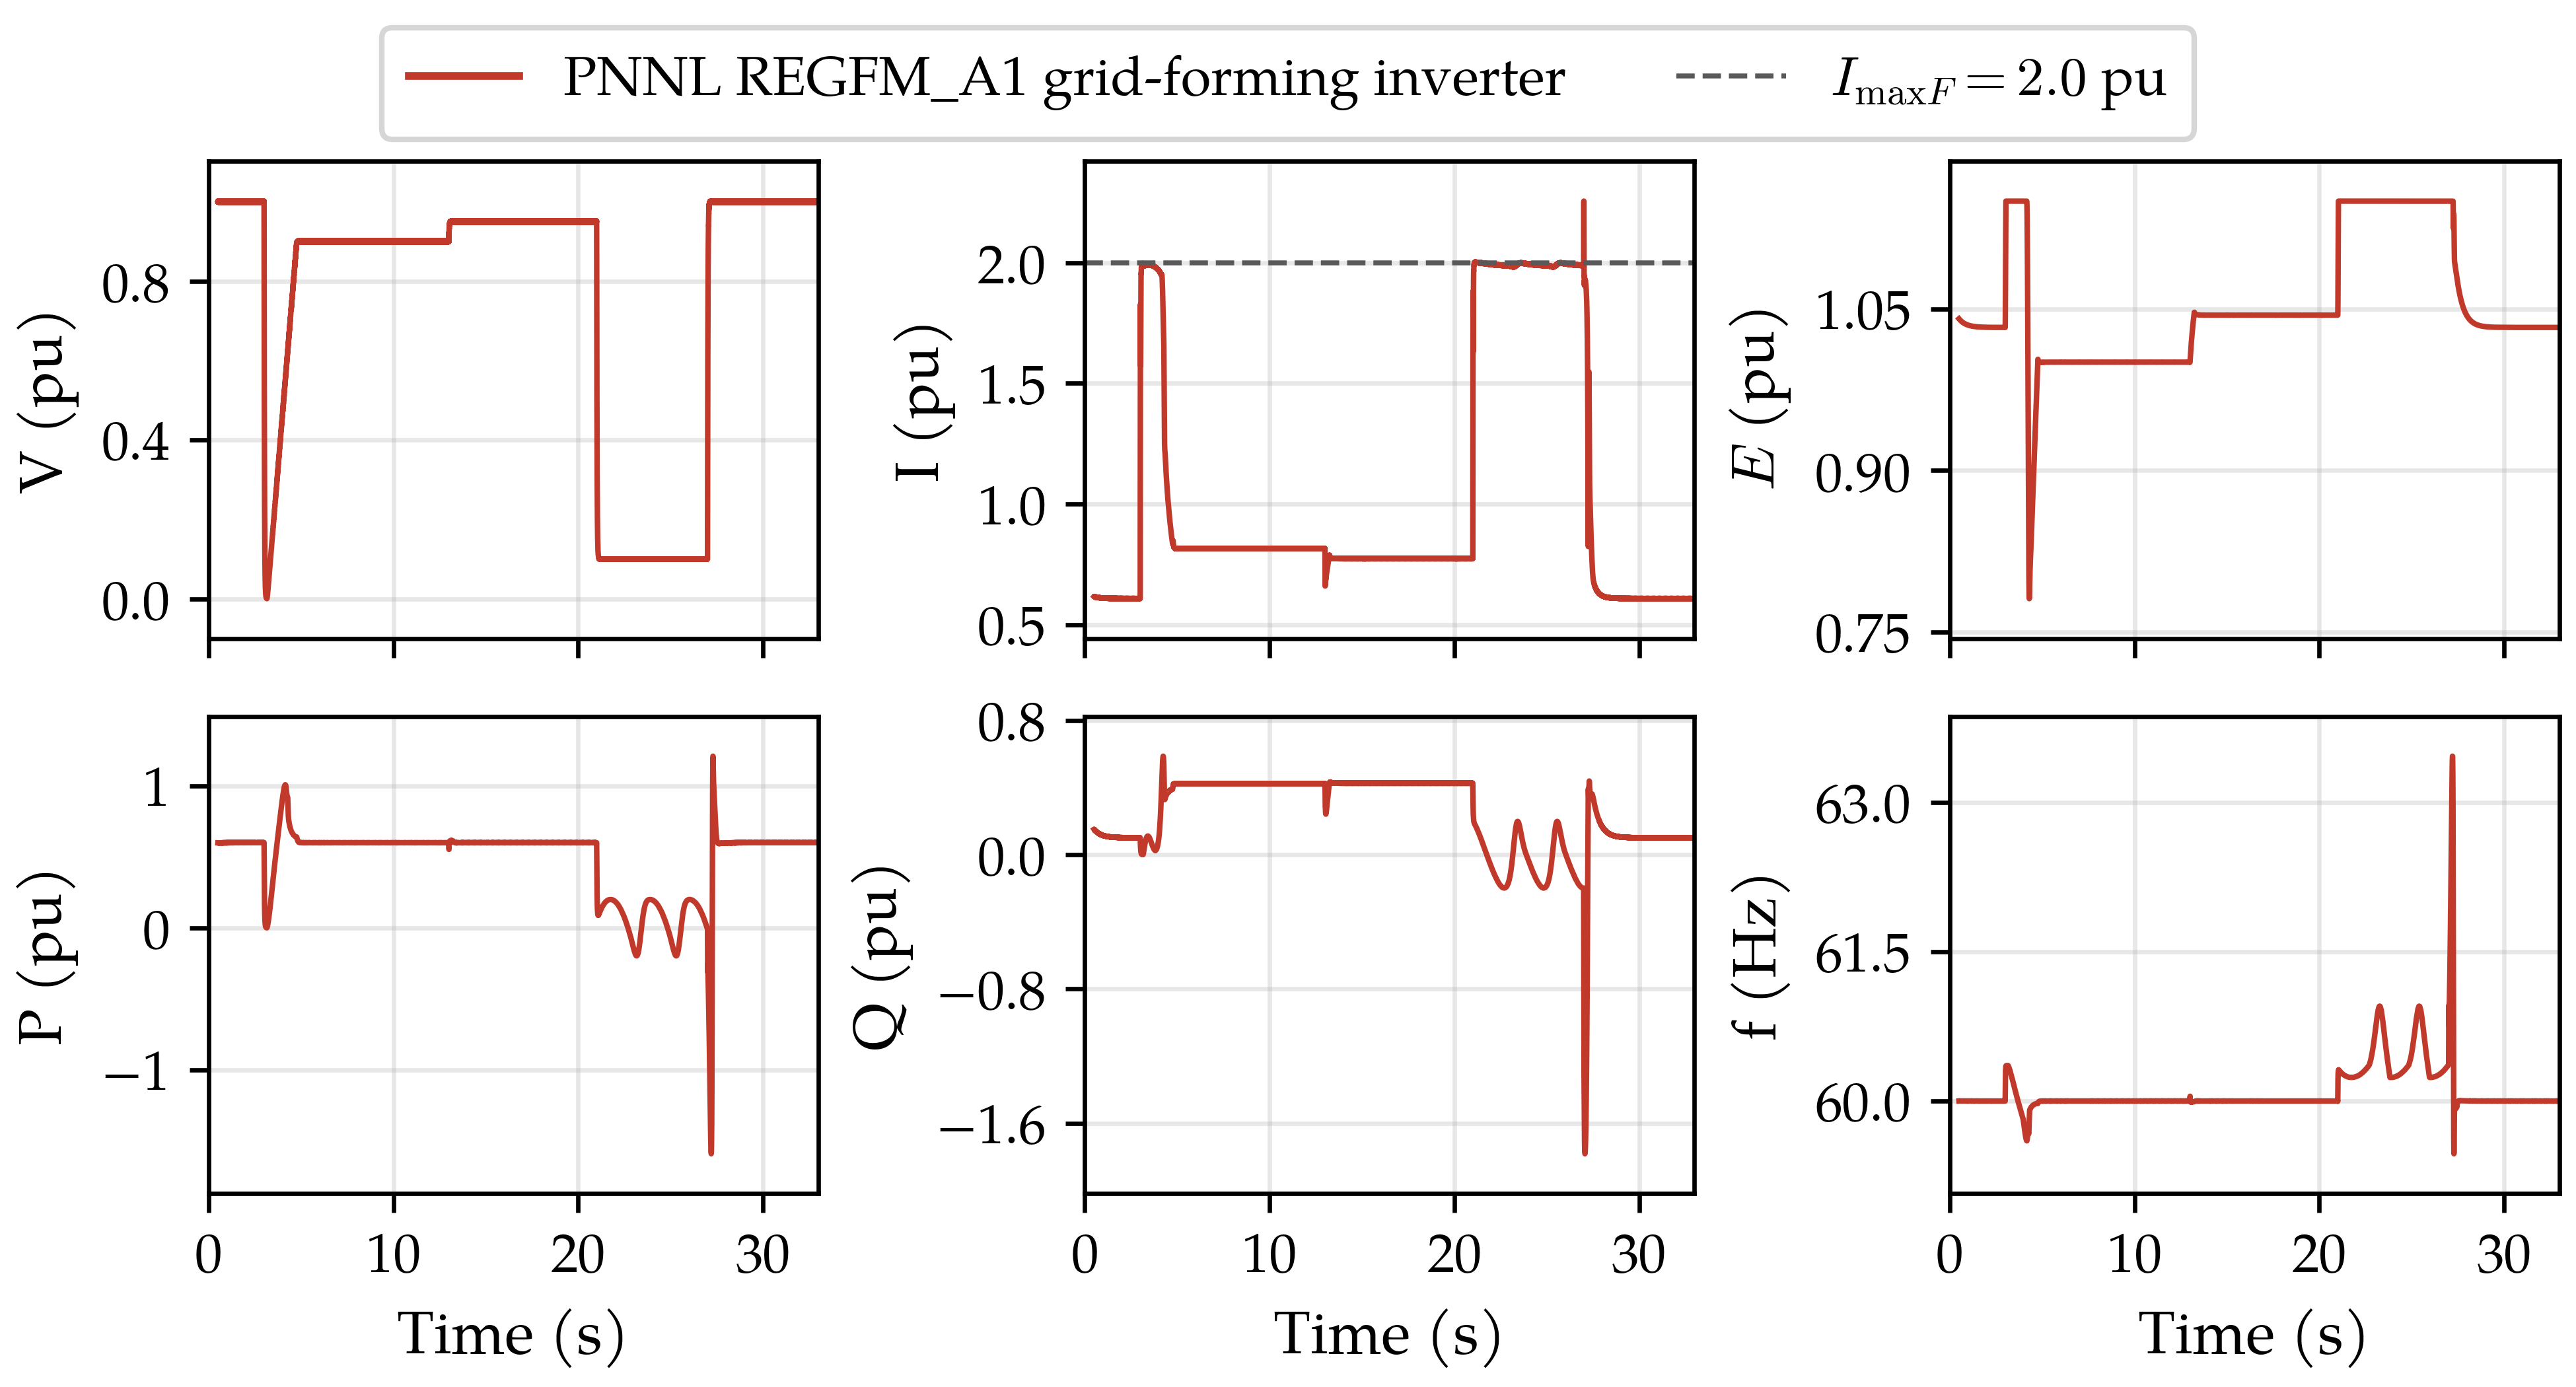
\includegraphics[width=\textwidth]{fig3_mqt_legacy_lvrt}
\caption{REGFM\_A1 response to the legacy low-voltage ride-through profile in PMView: source voltage, the inverter's internal current magnitude against its 2.0 per-unit transient limit, internal voltage magnitude, active and reactive power at the point of interconnection, and droop frequency.}
\label{fig:mqt}
\end{figure}

\begin{figure}[tbp]\centering
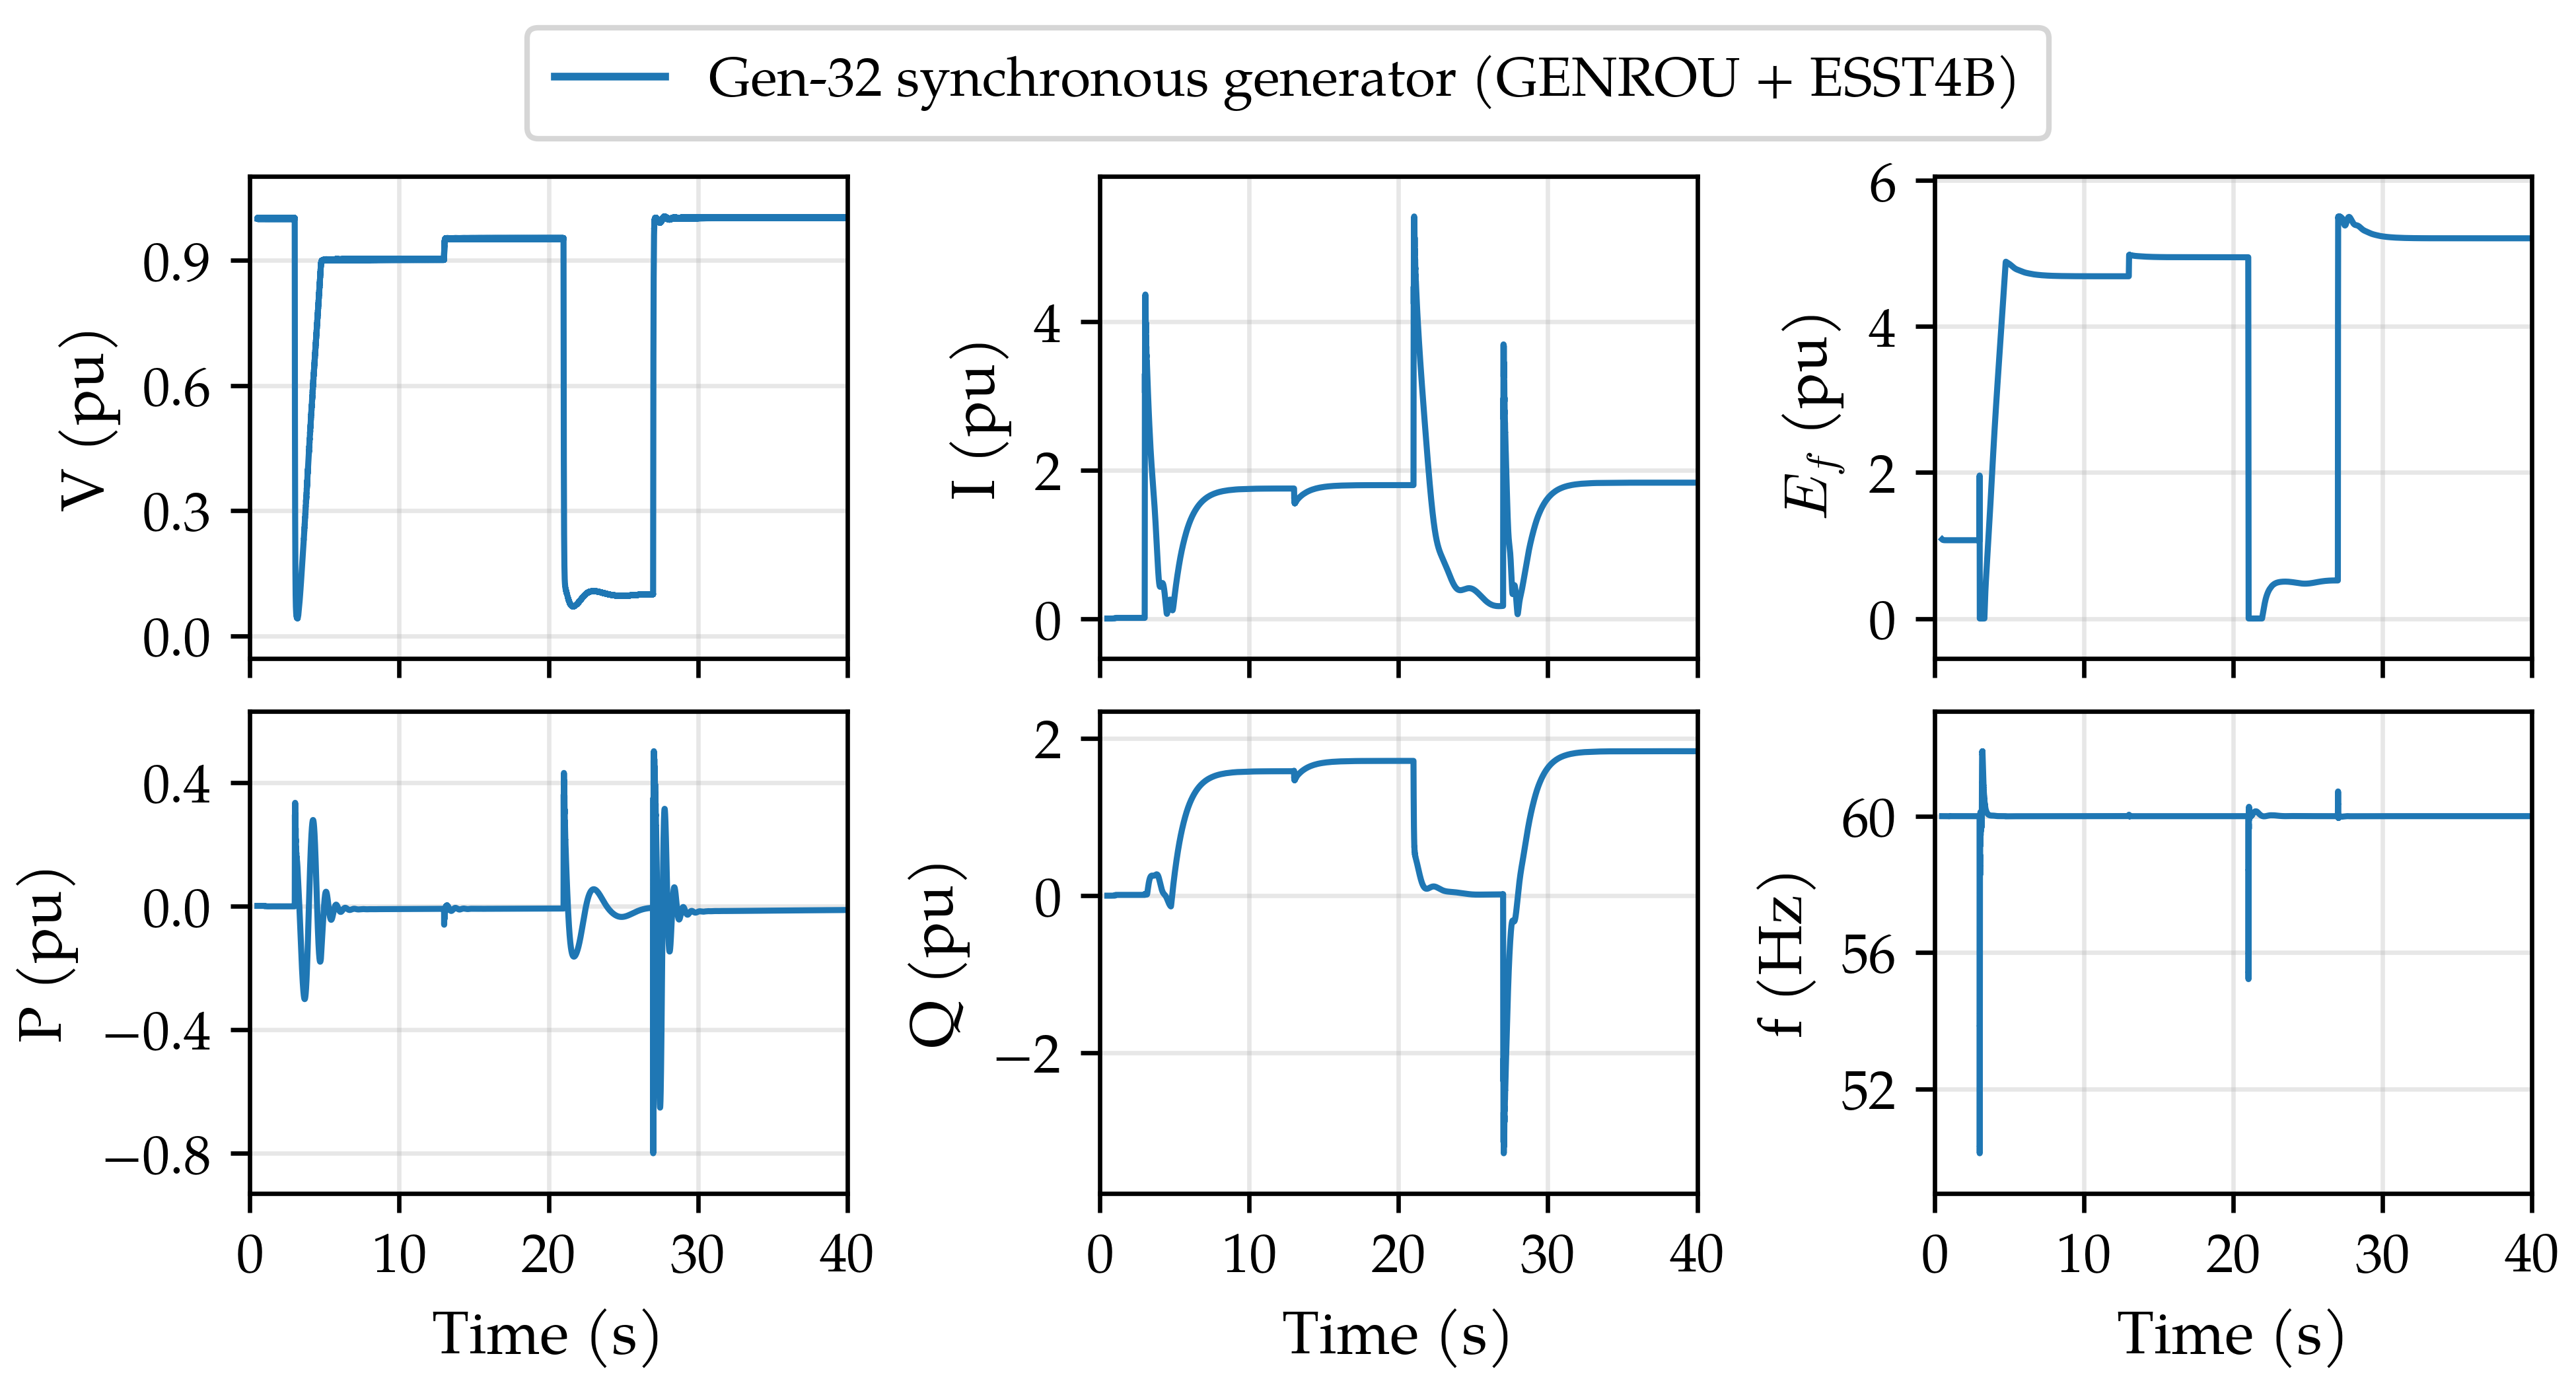
\includegraphics[width=\textwidth]{fig3_mqt_machine_lvrt}
\caption{Synchronous-machine response under the legacy low-voltage ride-through profile for the Gen-32 test case.}
\label{fig:mqtmachine}
\end{figure}

\begin{figure}[tbp]\centering
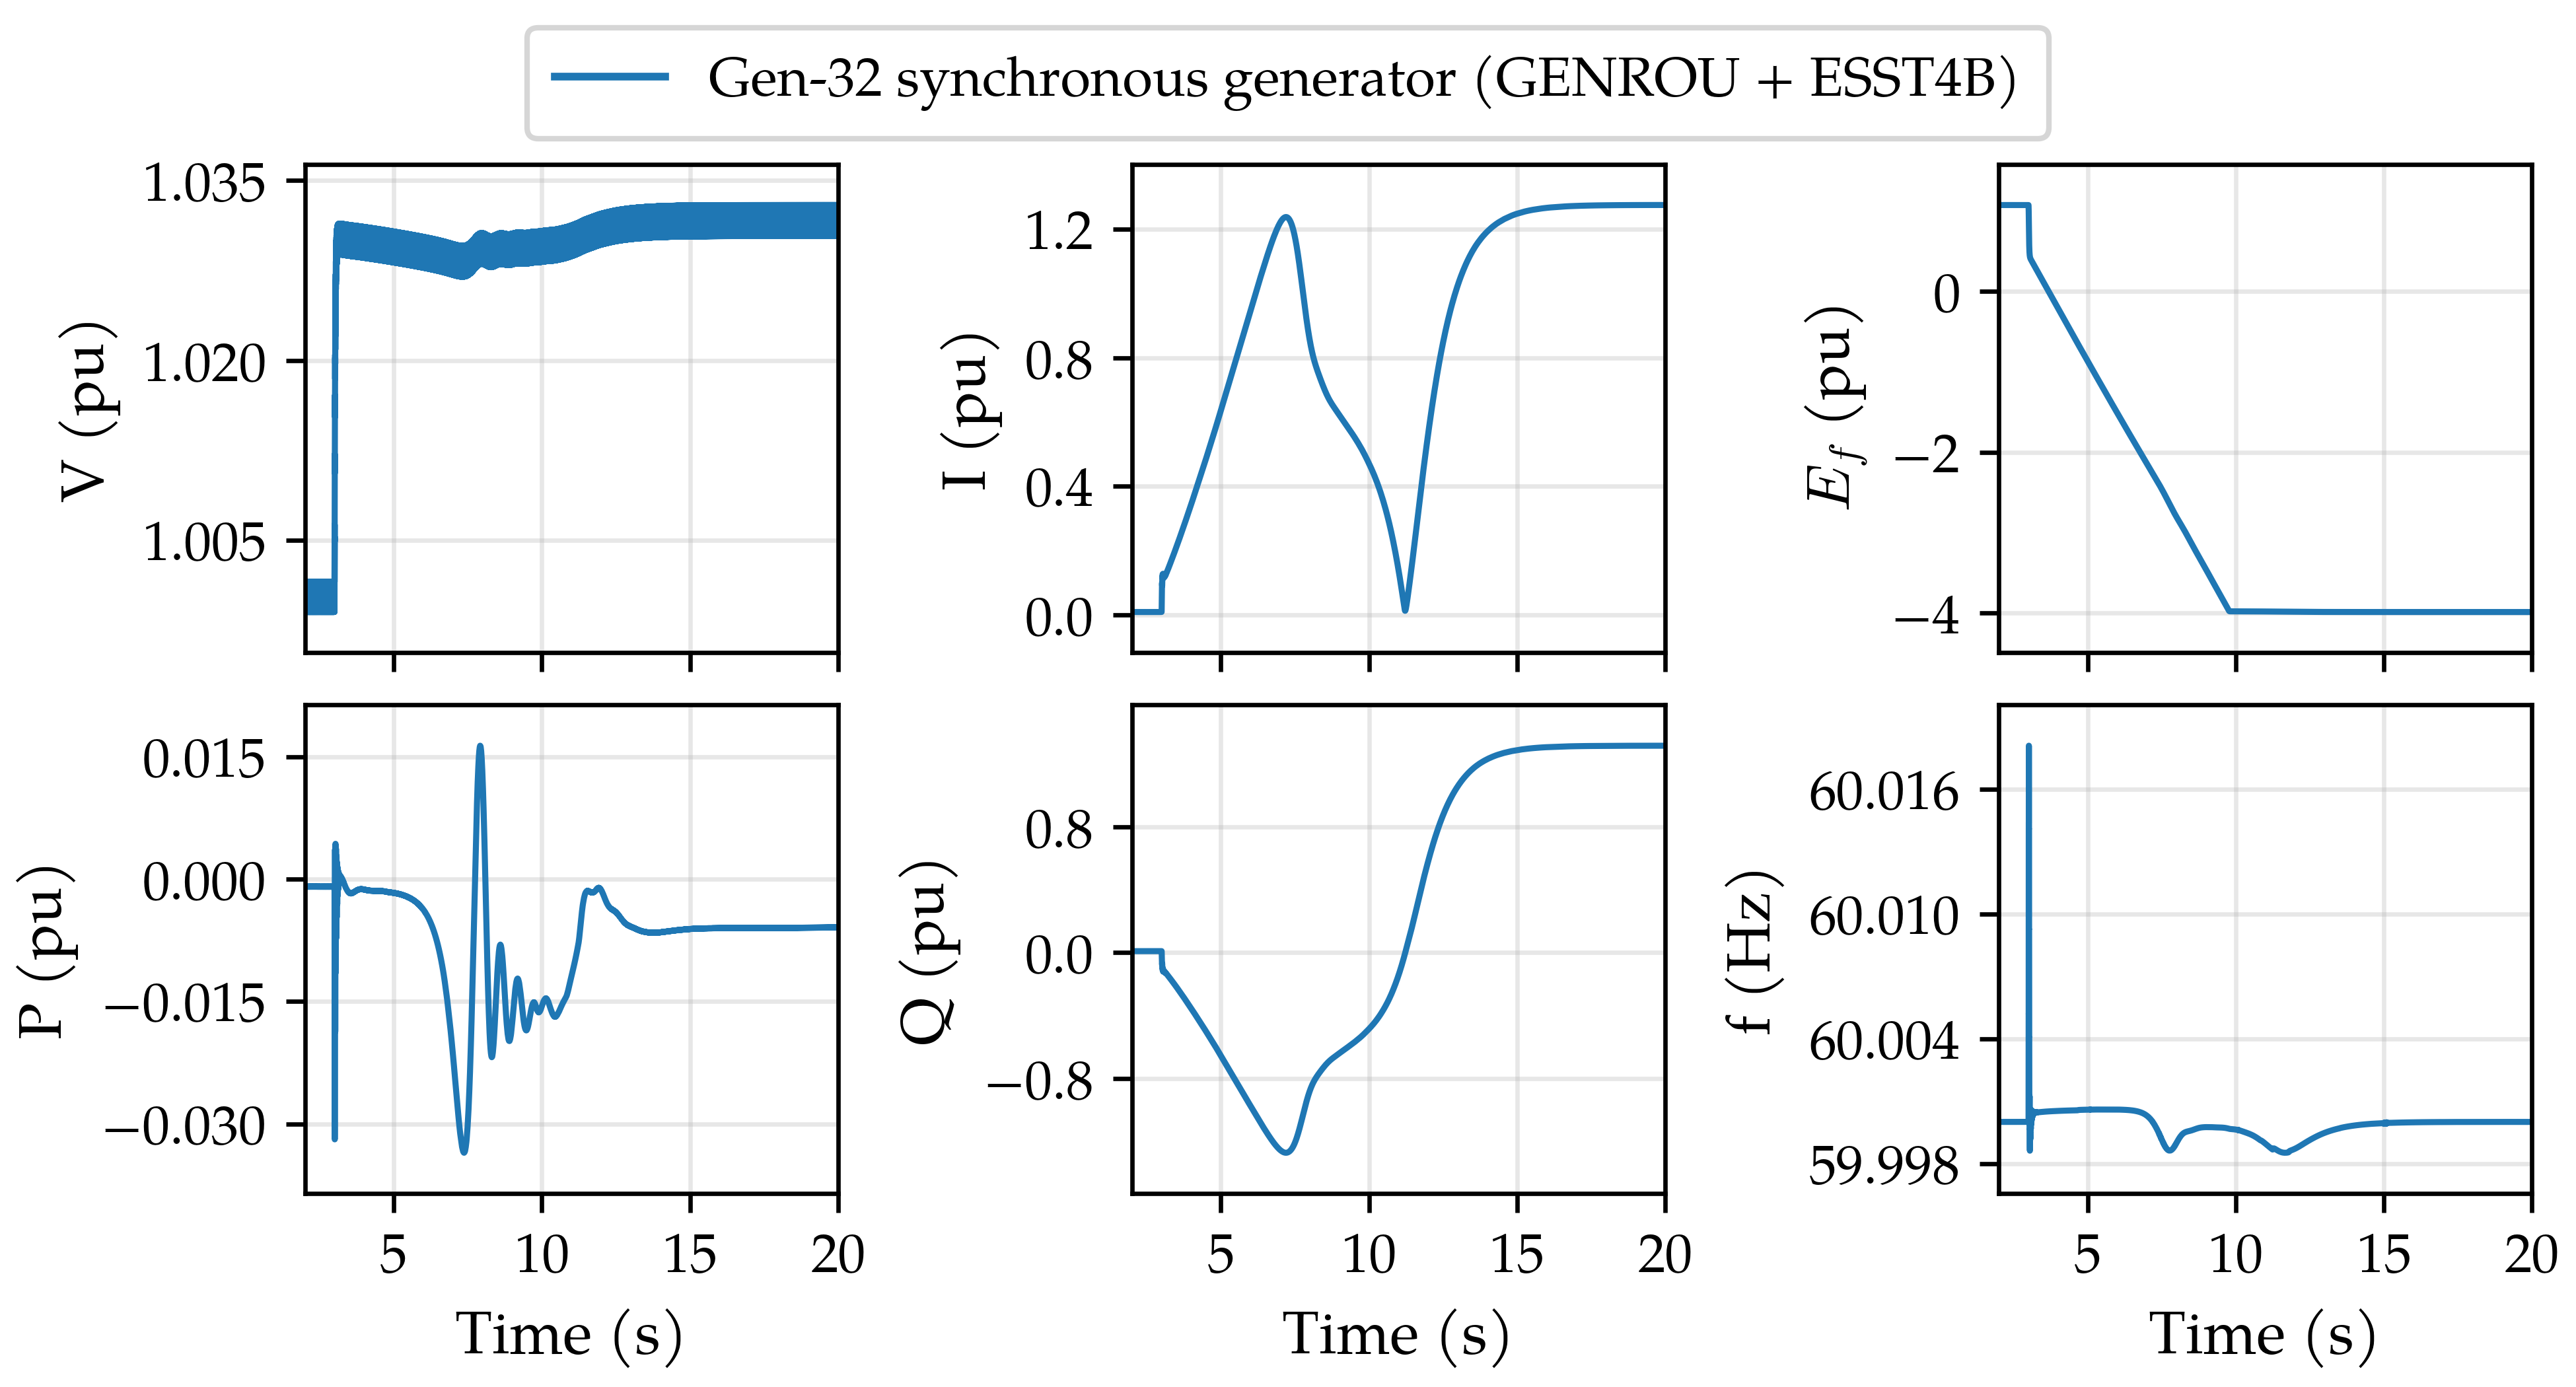
\includegraphics[width=\textwidth]{fig3_mqt_machine_vstep}
\caption{Gen-32 response to a source-voltage step from 1.00 to 1.03 per unit at 3~s.}
\label{fig:mqtmachinestep}
\end{figure}

\begin{figure}[tbp]\centering
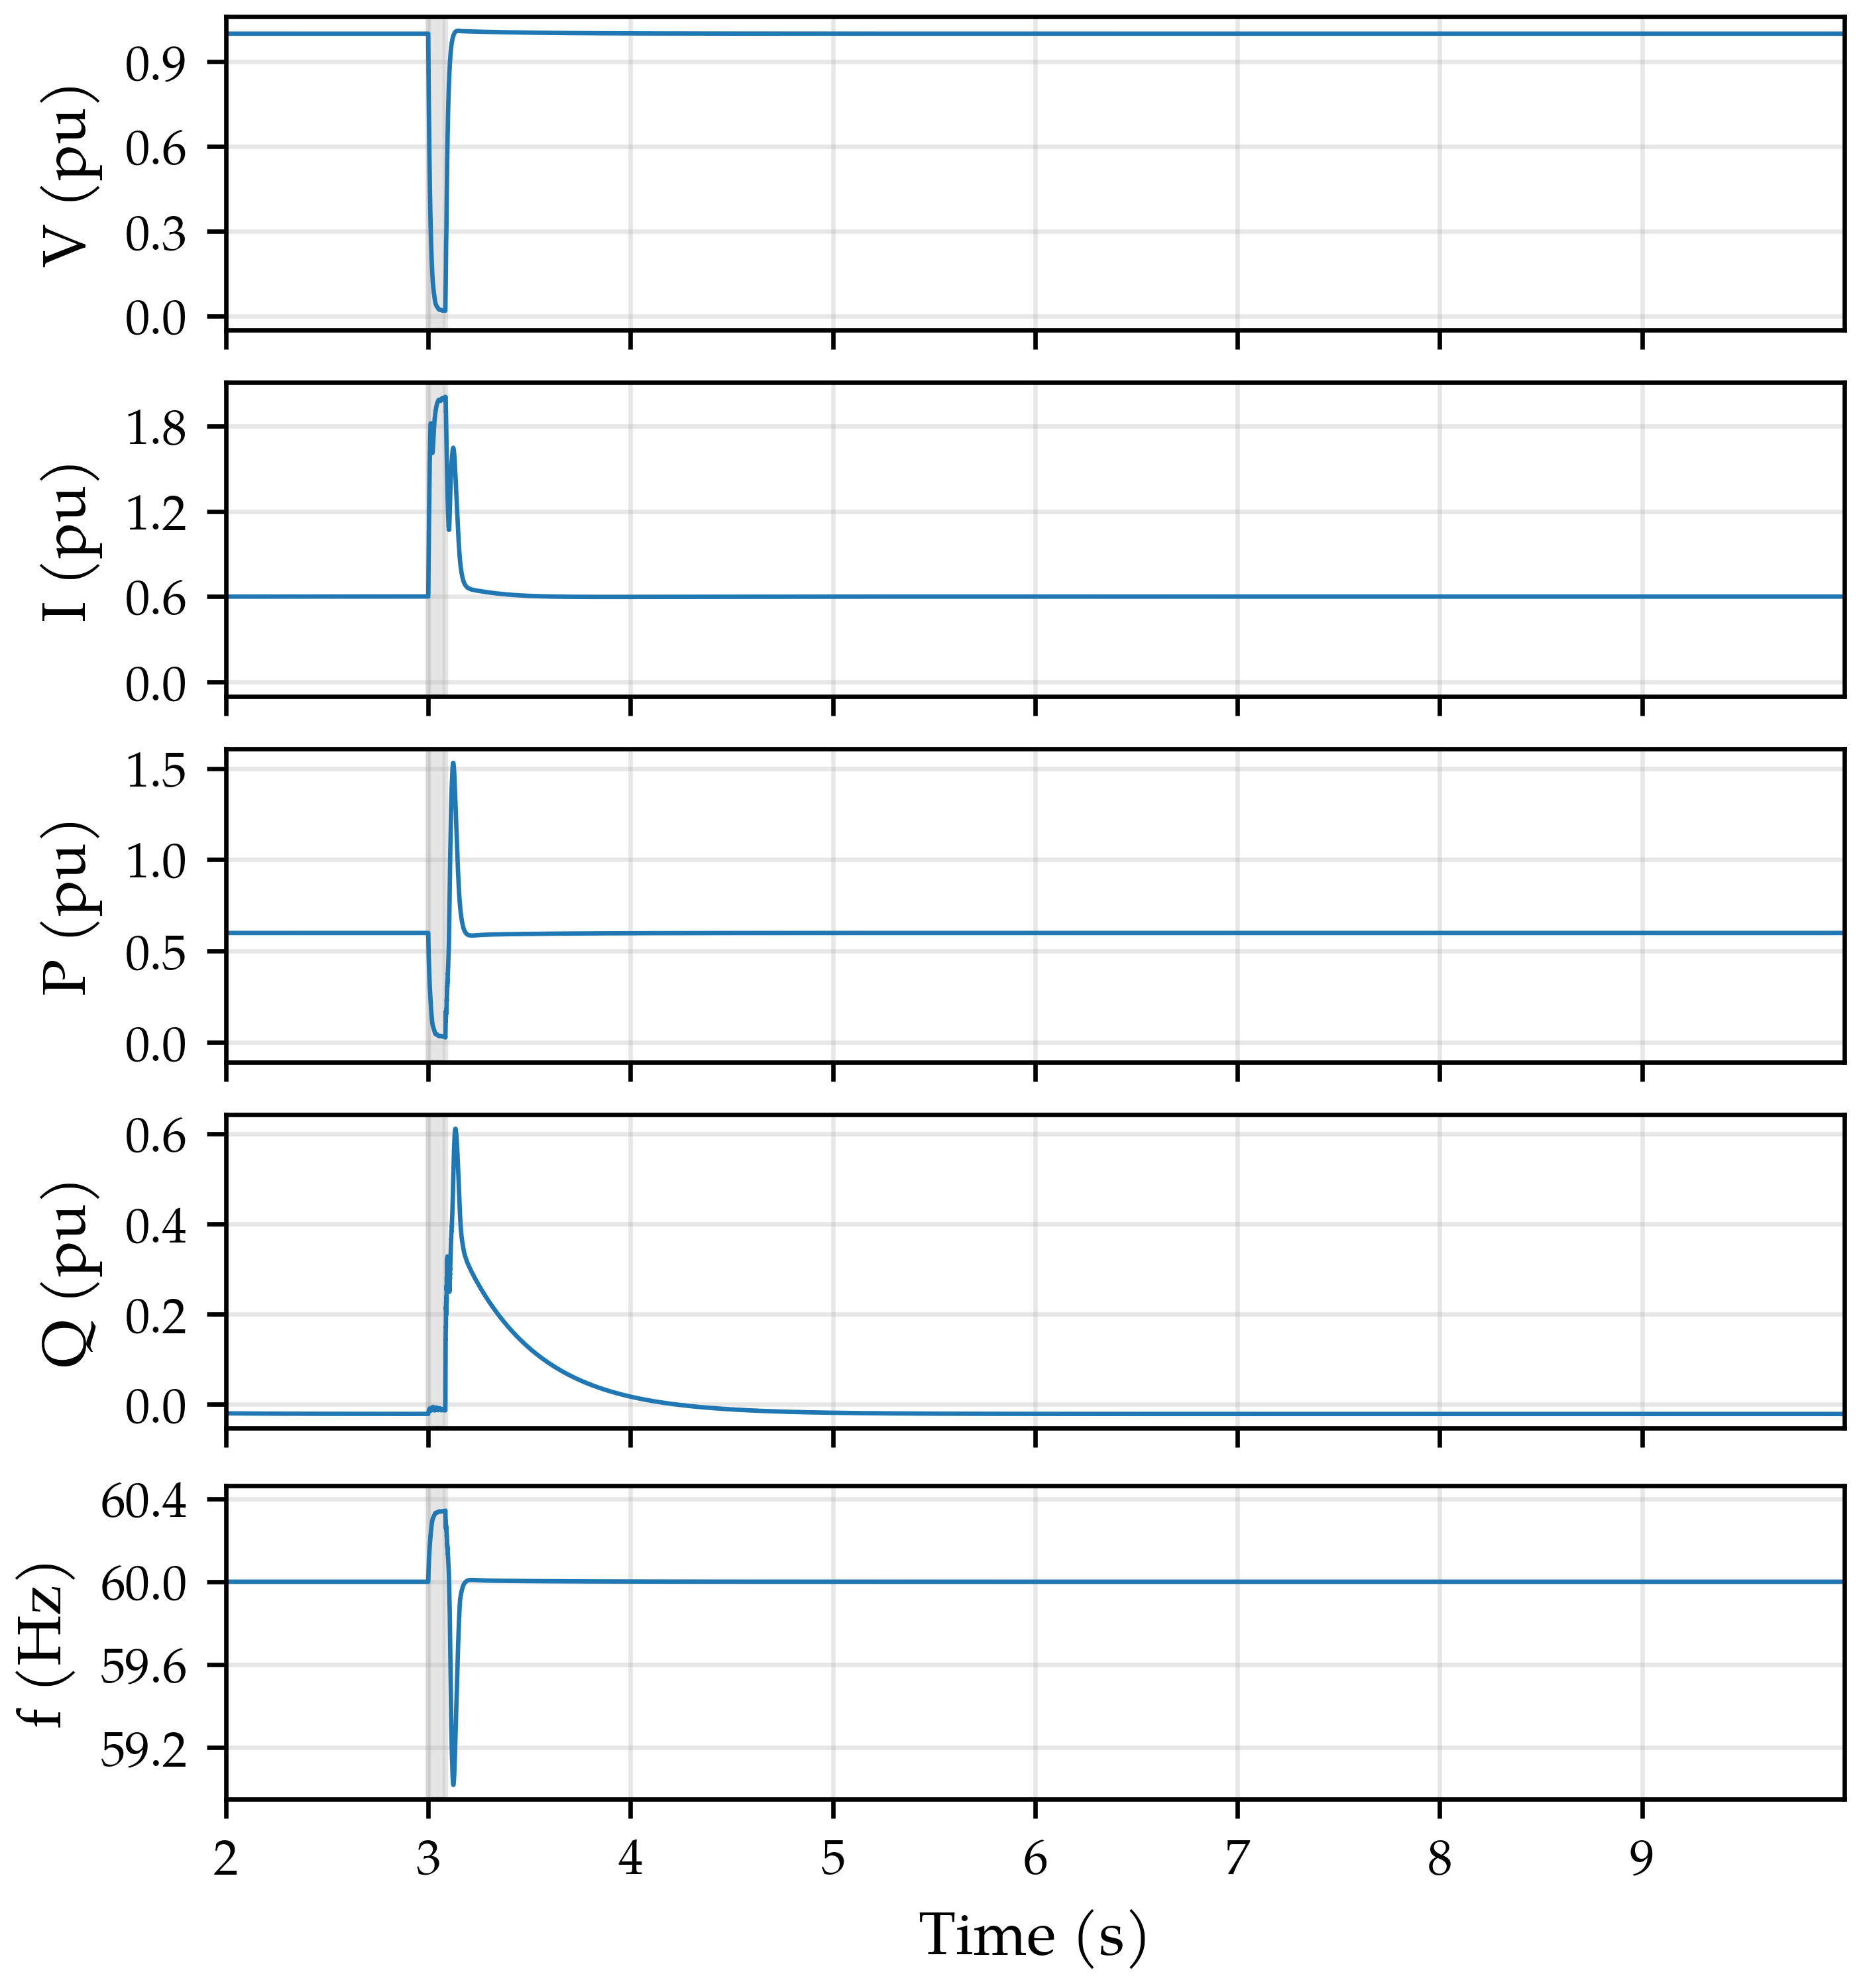
\includegraphics[width=0.72\textwidth]{fig7_smib_gfm_panel}
\caption{Single REGFM\_A1 response to a five-cycle bolted three-phase fault at its point of interconnection, with a 2.0 per-unit transient-current limit: the model's per-unit voltage, current, active and reactive powers, and its droop frequency in Hz.}
\label{fig:smibgfm}
\end{figure}

\subsection{Study Design}
\label{sec:studydesign}
We first applied a three-phase-to-ground fault at bus~14 to the all-machine IEEE-39-bus system. The fault resistance is 0.01~$\Omega$, a low-impedance approximation to a bolted fault. Initial machine studies considered both restoration of the faulted connection and clearing with the connection left open. The reference case used for the replacement progression has a five-cycle fault without reclosing logic configured.

We selected a short reference disturbance to represent a practical protection timescale. The 0.0833~s duration corresponds to approximately five cycles at 60~Hz and is applied from 3.0~s. After establishing the machine baseline fault-ride-through behavior, we replaced machines with GFM units dispatched at the same active and reactive power operating points as the machines. We replaced each synchronous generator, machine, one at a time and reapplied the same reference 5 cycle, 3 phase to ground fault. Extended-duration tests discussed later explore transient stability limits rather than recommended protection operating times. Table~\ref{tab:cases} lists the simulated cases. Network faults were applied at buses~14, 13, 10, and~39. All faults in the replacement progression and the current-limit studies are three-phase-to-ground. Single-line-to-ground and double-line-to-ground faults at bus~14 are reported in Section~\ref{sec:unbal}. Instantaneous failures of the semiconductor switches, which occur on a much faster timescale than the control limiter, are not represented in any case other than the grid-following inverter test case, which does not ride through the applied disturbance.

\begin{table}[tbp]\centering\small
\caption{Simulated fault cases. Fault resistance 0.01~$\Omega$; fault applied at 3.0~s.}
\label{tab:cases}
\begin{tabular}{>{\raggedright\arraybackslash}p{0.26\linewidth}>{\raggedright\arraybackslash}p{0.19\linewidth}>{\raggedright\arraybackslash}p{0.11\linewidth}>{\raggedright\arraybackslash}p{0.19\linewidth}>{\raggedright\arraybackslash}p{0.11\linewidth}}\toprule
Study & Configurations & Fault bus & Duration; clearing & GFM $I_{\max F}$\\\midrule
Replacement progression (Section~\ref{sec:emt}) & 0--10 GFM units & 14 & 5 cycles; lines to bus~14 opened, no reclosing & 2.0\\
Current-limit comparison & 0 and 10 GFM units & 10 & 5 cycles; lines to bus~10 opened, no reclosing & 1.5\\
Fault at a unit's transmission bus (Section~\ref{sec:emt}) & 0 and 10 GFM units & 39 & 5 cycles; lines 1--39 and 9--39 opened, no reclosing, so the bus-39 unit islands with the bus-39 load & 1.5\\
Current-limit sensitivity (Section~\ref{sec:emt}) & 10 GFM units & 14 & 5 cycles; lines to bus~14 opened, no reclosing & 2.0; 1.5; 1.2; 1.1\\
Current-limit sensitivity, near fault (Section~\ref{sec:emt}) & 10 GFM units & 13 & 5 cycles; lines 10--13 and 13--14 opened, no reclosing & 15; 2.0; 1.5; 1.2; 1.1; 1.0\\
Unbalanced-fault check (Section~\ref{sec:unbal}) & 0 and 10 GFM units & 14 & 5 cycles, single-line-to-ground and double-line-to-ground; lines to bus~14 opened, no reclosing & 2.0\\
Single-device comparison (Section~\ref{sec:dynamics}) & one machine; one inverter; infinite bus, SCR~10 & point of interconnection & 5 cycles; self-clearing & 2.0\\
Clearing-time limits (Section~\ref{sec:energymethod}) & ten machines; ten GFM units; one machine; one inverter & 14; point of interconnection & duration swept; self-clearing, network intact & 2.0; 2.0--15 (single inverter)\\\bottomrule
\end{tabular}
\end{table}

\subsection{PSCAD Automation}
\label{sec:automation}
We configured and ran the one-for-one replacement cases manually. For subsequent model-quality studies, we used PSCAD's \texttt{mhi.pscad} Python interface to launch PSCAD, load the case, modify parameters, and export results. Component identifiers locate the fault application time, duration, resistance, solution step, and run length. Each run writes a separate directory named for the varied parameter and stores the exported channels with its fault configuration and device parameters.

The automation sets parameters before launching each simulation and collects the output channels after completion. A written configuration accompanies each run so that a parameter sweep can be interpreted as a sequence of distinct test cases. We used this workflow for repeated device tests while retaining the manually configured replacement cases as the network-study starting point.

\subsection{Data Processing}
\label{sec:pipeline}
At the end of a run, PSCAD writes numbered \texttt{.out} files containing whitespace-delimited numerical channels. The first column is time, followed by up to ten recorded channels, so a large case produces multiple files with repeated time columns. A companion \texttt{.inf} file supplies the global channel indices, descriptions, groups, limits, and units.

The processing pipeline reads the \texttt{.inf} file and reconstructs the mapping from channel indices to the numbered output files. It then combines the channels into a common time-indexed table. Descriptions are not necessarily unique: different phases or measurement locations can share the same name. The pipeline distinguishes these descriptions before exporting CSV files for analysis and plotting.

The plotting scripts read the resulting tables to draw the simulation responses. Screenshots, circuit diagrams, and analytical illustrations complement those numerical plots. Appendix~\ref{app:plotting} describes the file formats and plotting conventions. The workflow allows the same processing approach to serve both individual-device and network studies.

The simulation records behind the figures, the processing and plotting scripts, the figure data, and the PSCAD test systems are in the project's public repository \cite{ut26xrepo}. The PNNL REGFM\_A1 model used throughout, together with the REGFM\_B1, REGFM\_C1, and REPCGFM\_C1 models of the same family, is publicly available in PNNL's release of the WECC grid-forming inverter models \cite{pnnlgithub}.

\section{Simulation Testbed Results}
\label{sec:emt}
The results compare fault recovery as machines are replaced by GFM inverters and examine the role of current limiting. We used PSCAD~5.0.2 with GFortran~4.6 and the E-TRAN library for the converted IEEE 39-bus network \cite{etranlib}. The REGFM\_A1 model uses the PNNL library \texttt{PNNL\_REGFM\_A1\_gf46.lib} \cite{regfma1lib}. The fault-sweep cases use a 50~$\mu$s solution time step.

The reference fault begins at 3.0~s and lasts five cycles. Figure~\ref{fig:vrms12gfm} shows the first two steps of the replacement progression, with one and two machines replaced. Figure~\ref{fig:pscadallgfm} shows the all-GFM arrangement. The bus-14 reference study uses the 2.0 per-unit transient-current setting, while the separate bus-10 current-limit comparison uses 1.5 per unit. Clearing opens the breakers of the lines connected to bus~14 and isolates that bus: after clearing its active power, reactive power, and current are zero, and its plotted 30~kV is the residual voltage of the de-energized bus rather than a network-recovery quantity.

\begin{figure}[tbp]\centering
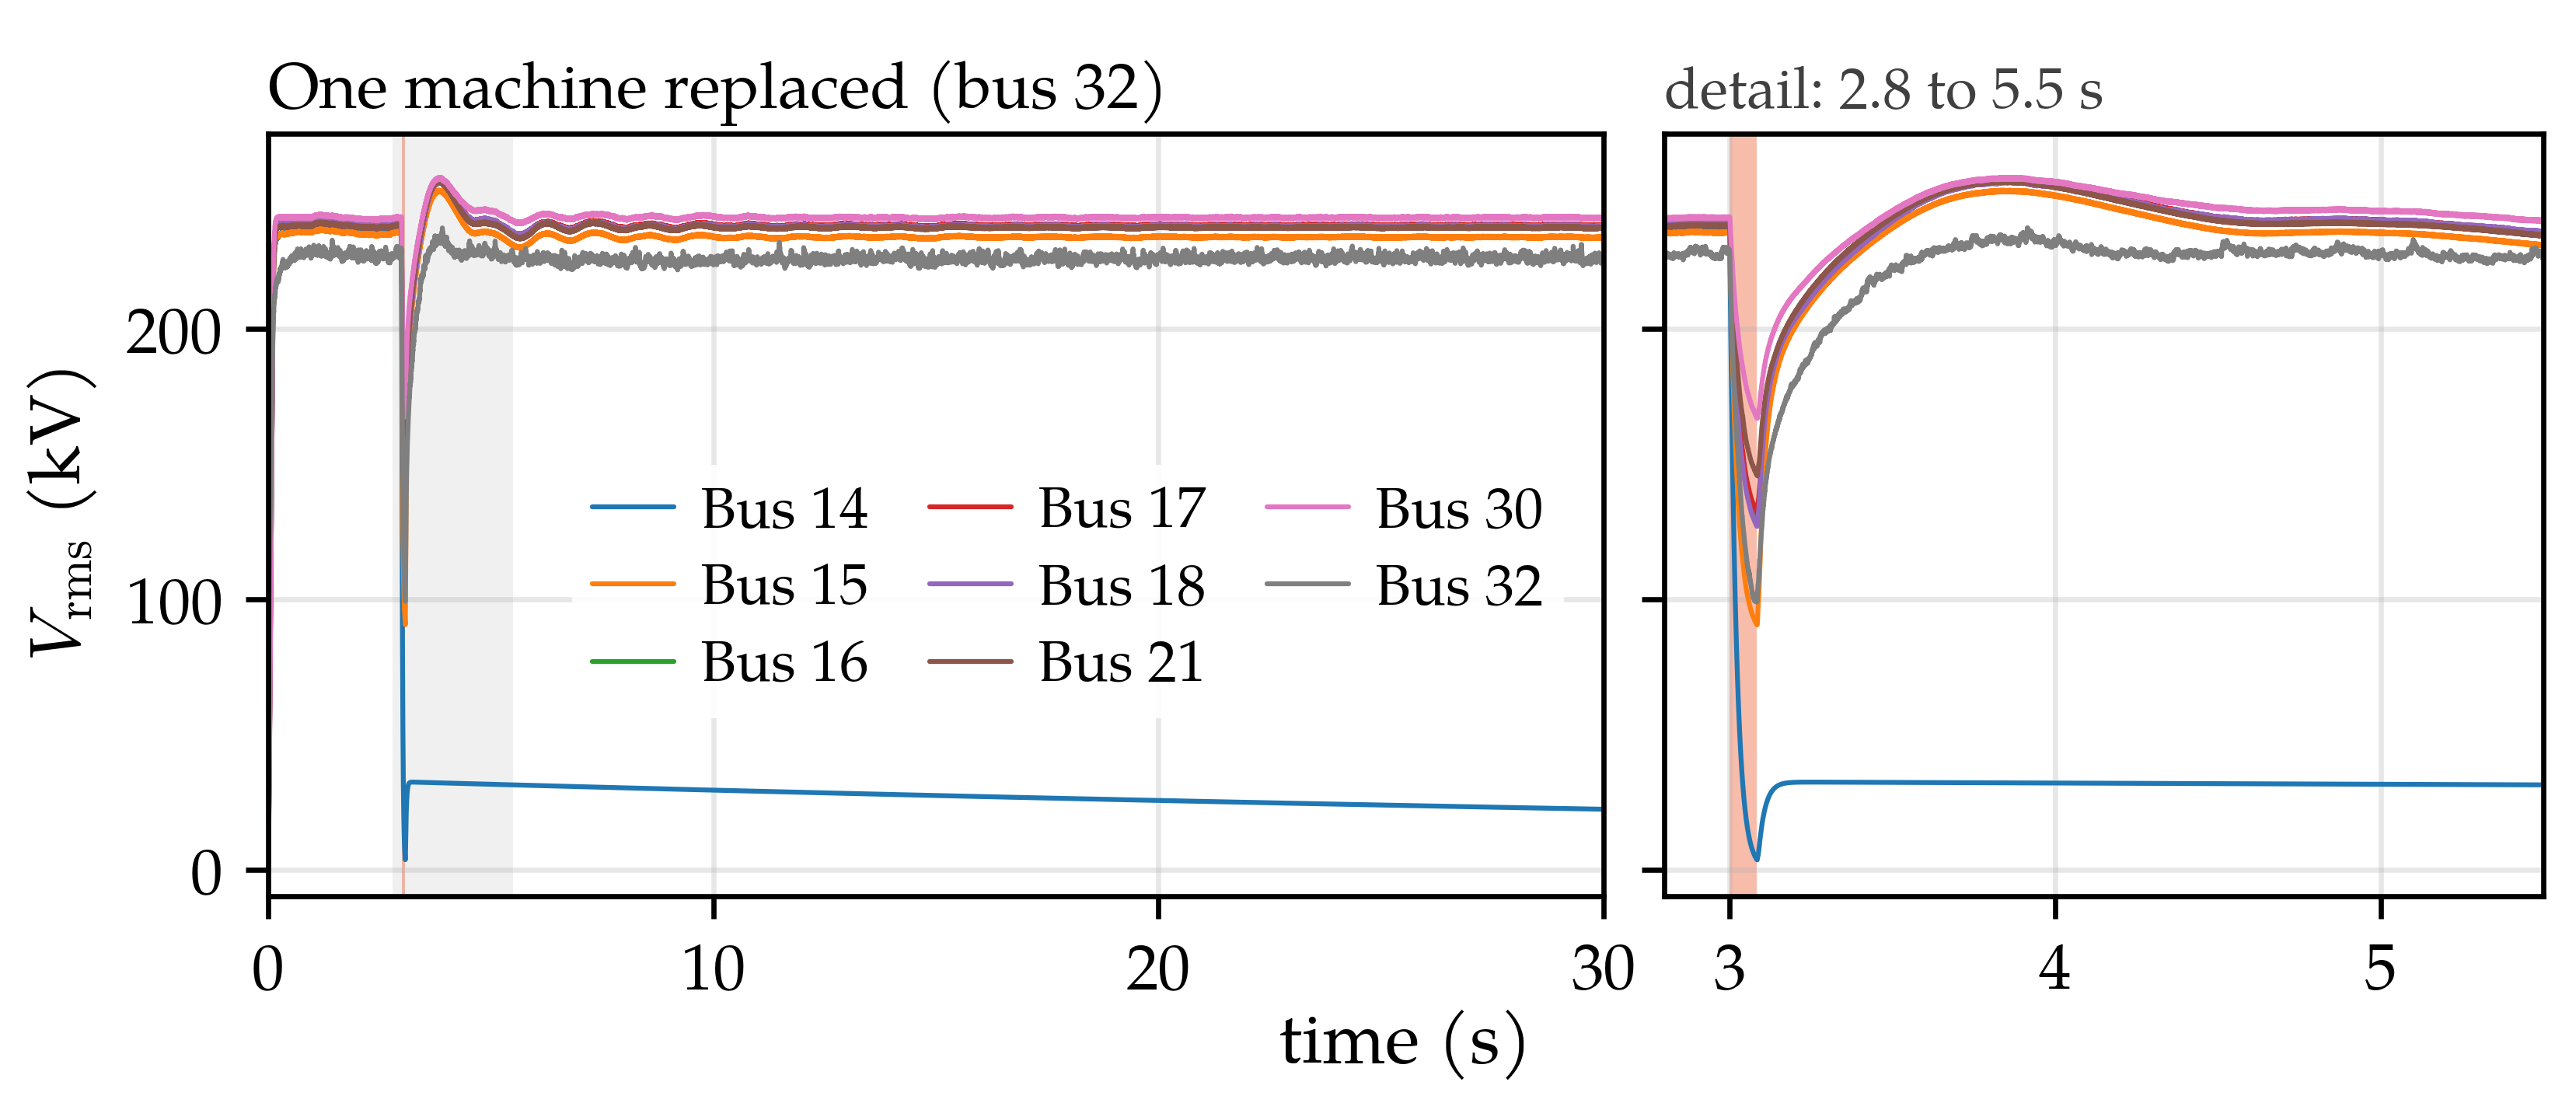
\includegraphics[width=0.85\textwidth]{vrms_1gfm}\\[4pt]
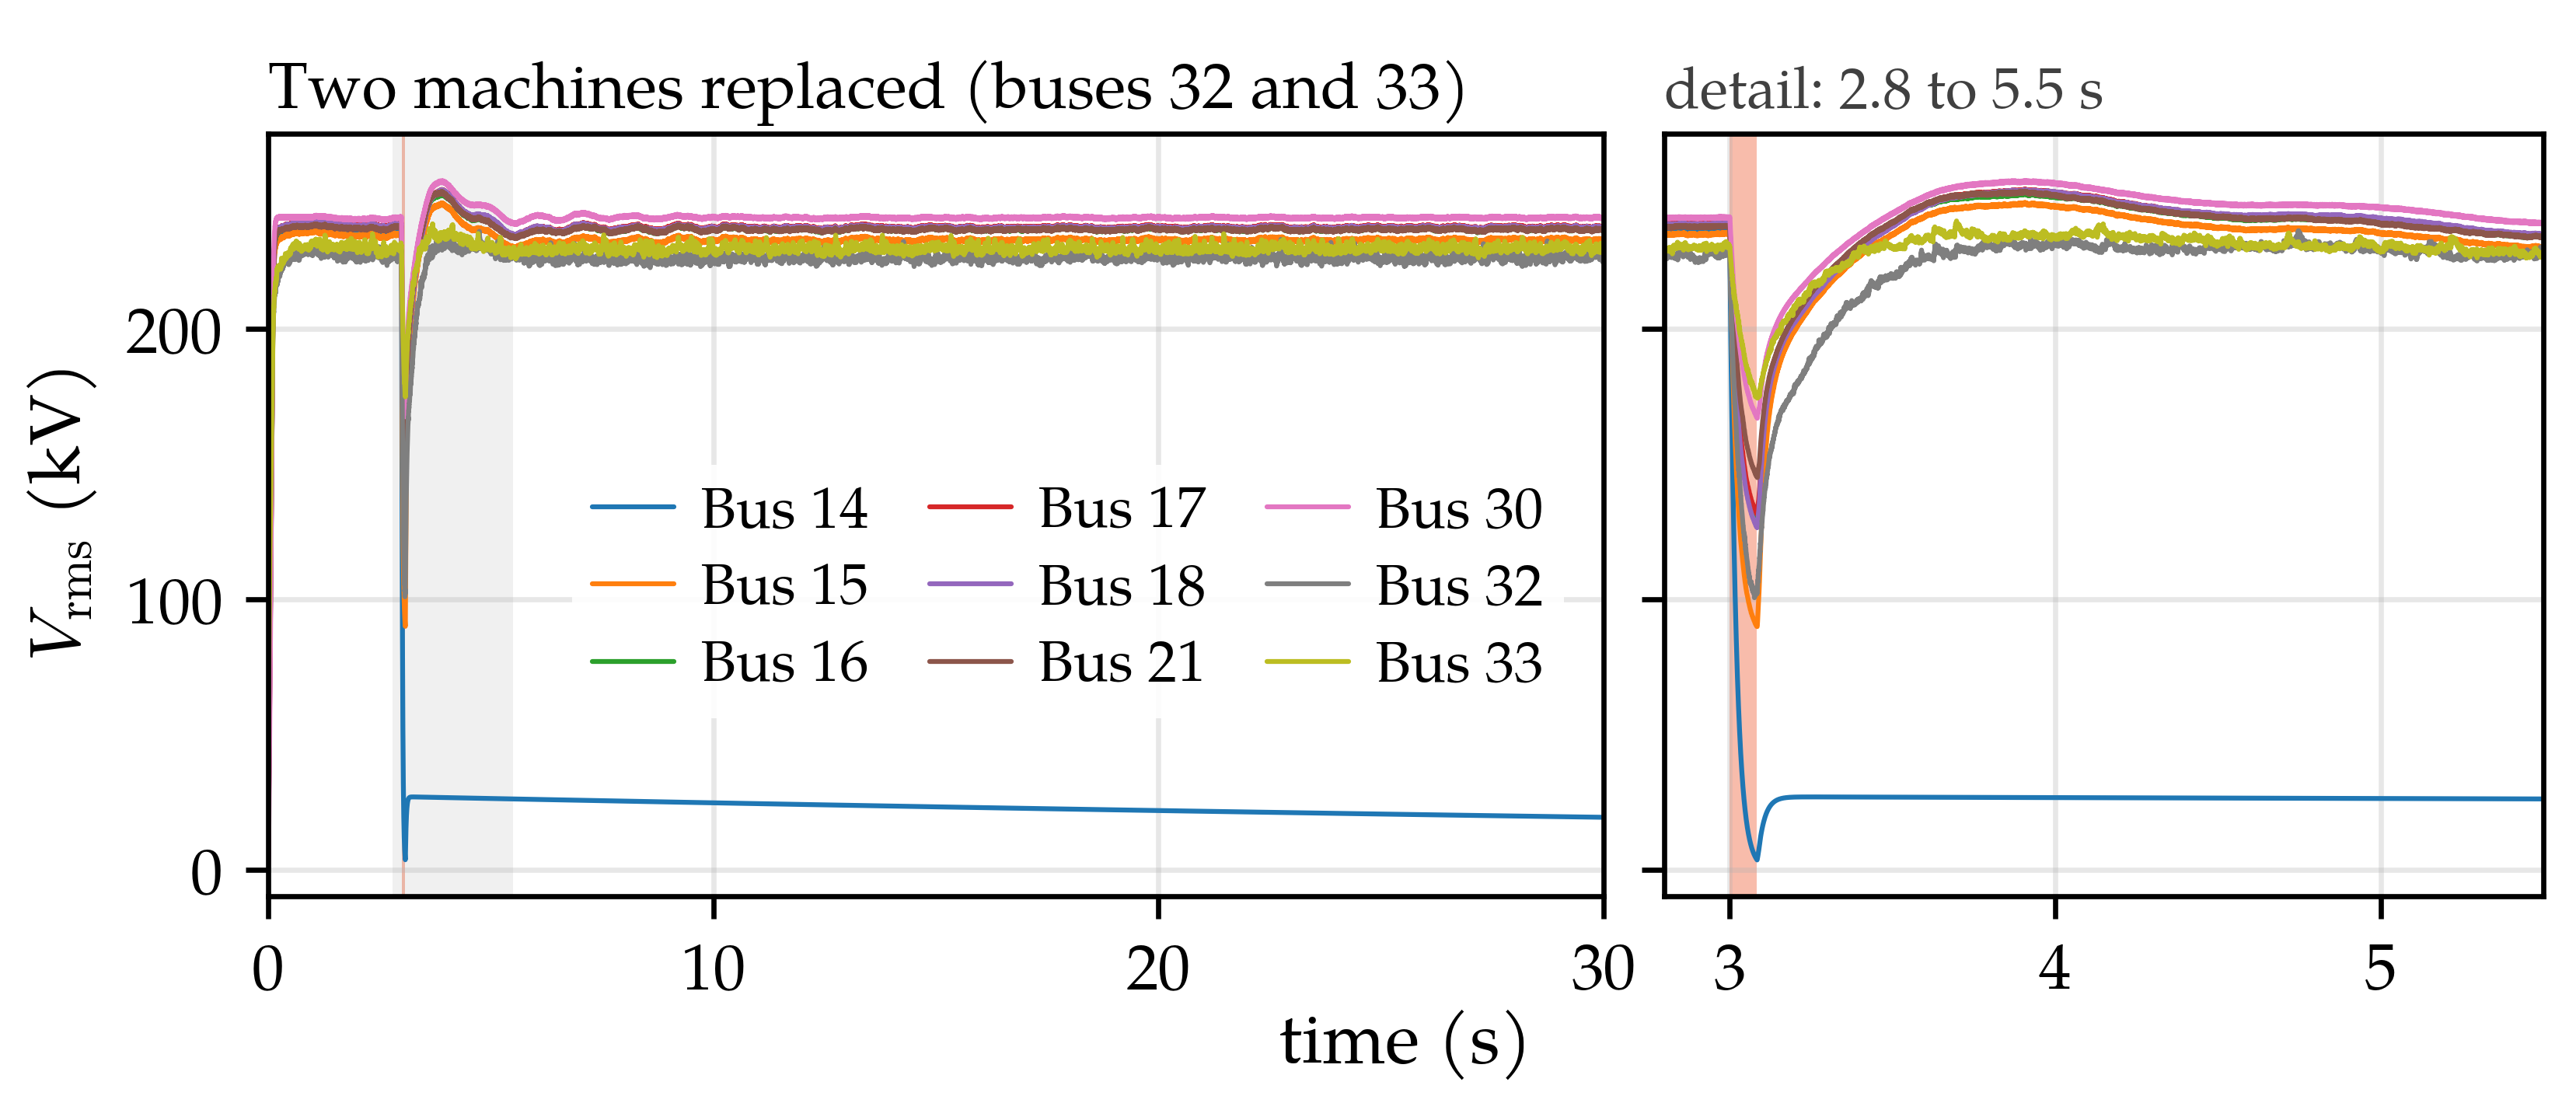
\includegraphics[width=0.85\textwidth]{vrms_2gfm}
\caption{Bus-voltage responses with one replaced machine (top) and two replaced machines (bottom) under the bus-14 reference fault; bus~14 is isolated by clearing, so its trace is the residual voltage of the de-energized bus.}
\label{fig:vrms12gfm}
\end{figure}

\begin{figure}[tbp]\centering
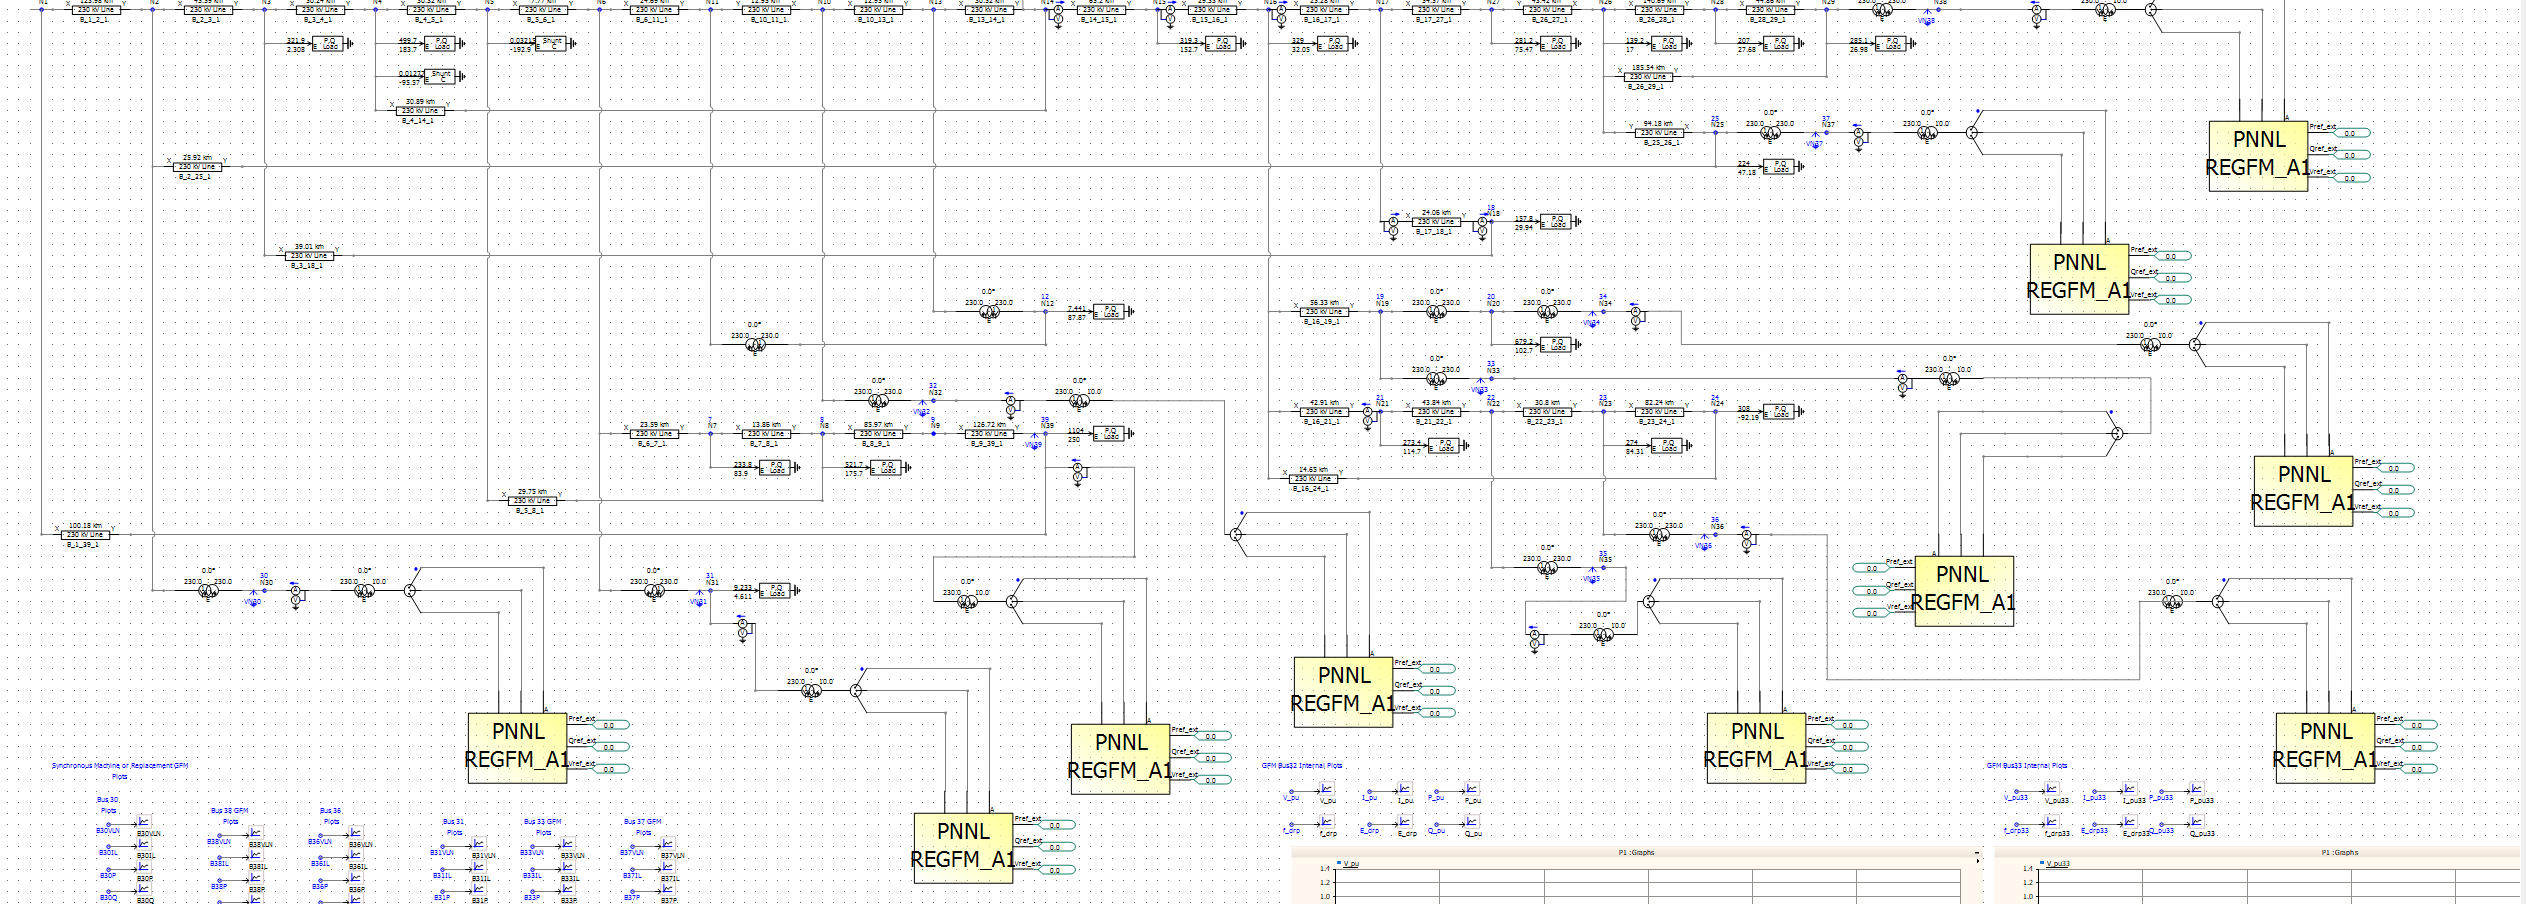
\includegraphics[width=\textwidth]{pscad_allgfm_39bus}
\caption{The fully inverter-based 39-bus network on the
PSCAD canvas: all ten machine subsystems replaced by PNNL REGFM\_A1
units (yellow blocks), each behind its step-up transformer, with the
per-bus signal taps and system plot panels.}
\label{fig:pscadallgfm}
\end{figure}

\subsection{Iterative Synchronous Machine Replacement}
The eleven replacement configurations show recovery of the connected network under the reference disturbance. Figures~\ref{fig:allgfm}--\ref{fig:sweep} compare the all-GFM response with the machine baseline and selected intermediate configurations. Breaker opening removes the faulted connection, and reclosing is disabled in the reference progression. Reclosing can be added through the testbed's breaker logic for other study conditions.

The selected GFM responses return promptly toward their post-fault operating points. The machine response contains longer oscillations, while the voltage and power trajectories also vary by location. Opening a line can change the post-fault operating point, so recovery need not return every quantity to its pre-fault value. The progression demonstrates mixed-resource studies under a common disturbance without assuming that every placement or dispatch behaves identically.

\begin{figure}[tbp]\centering
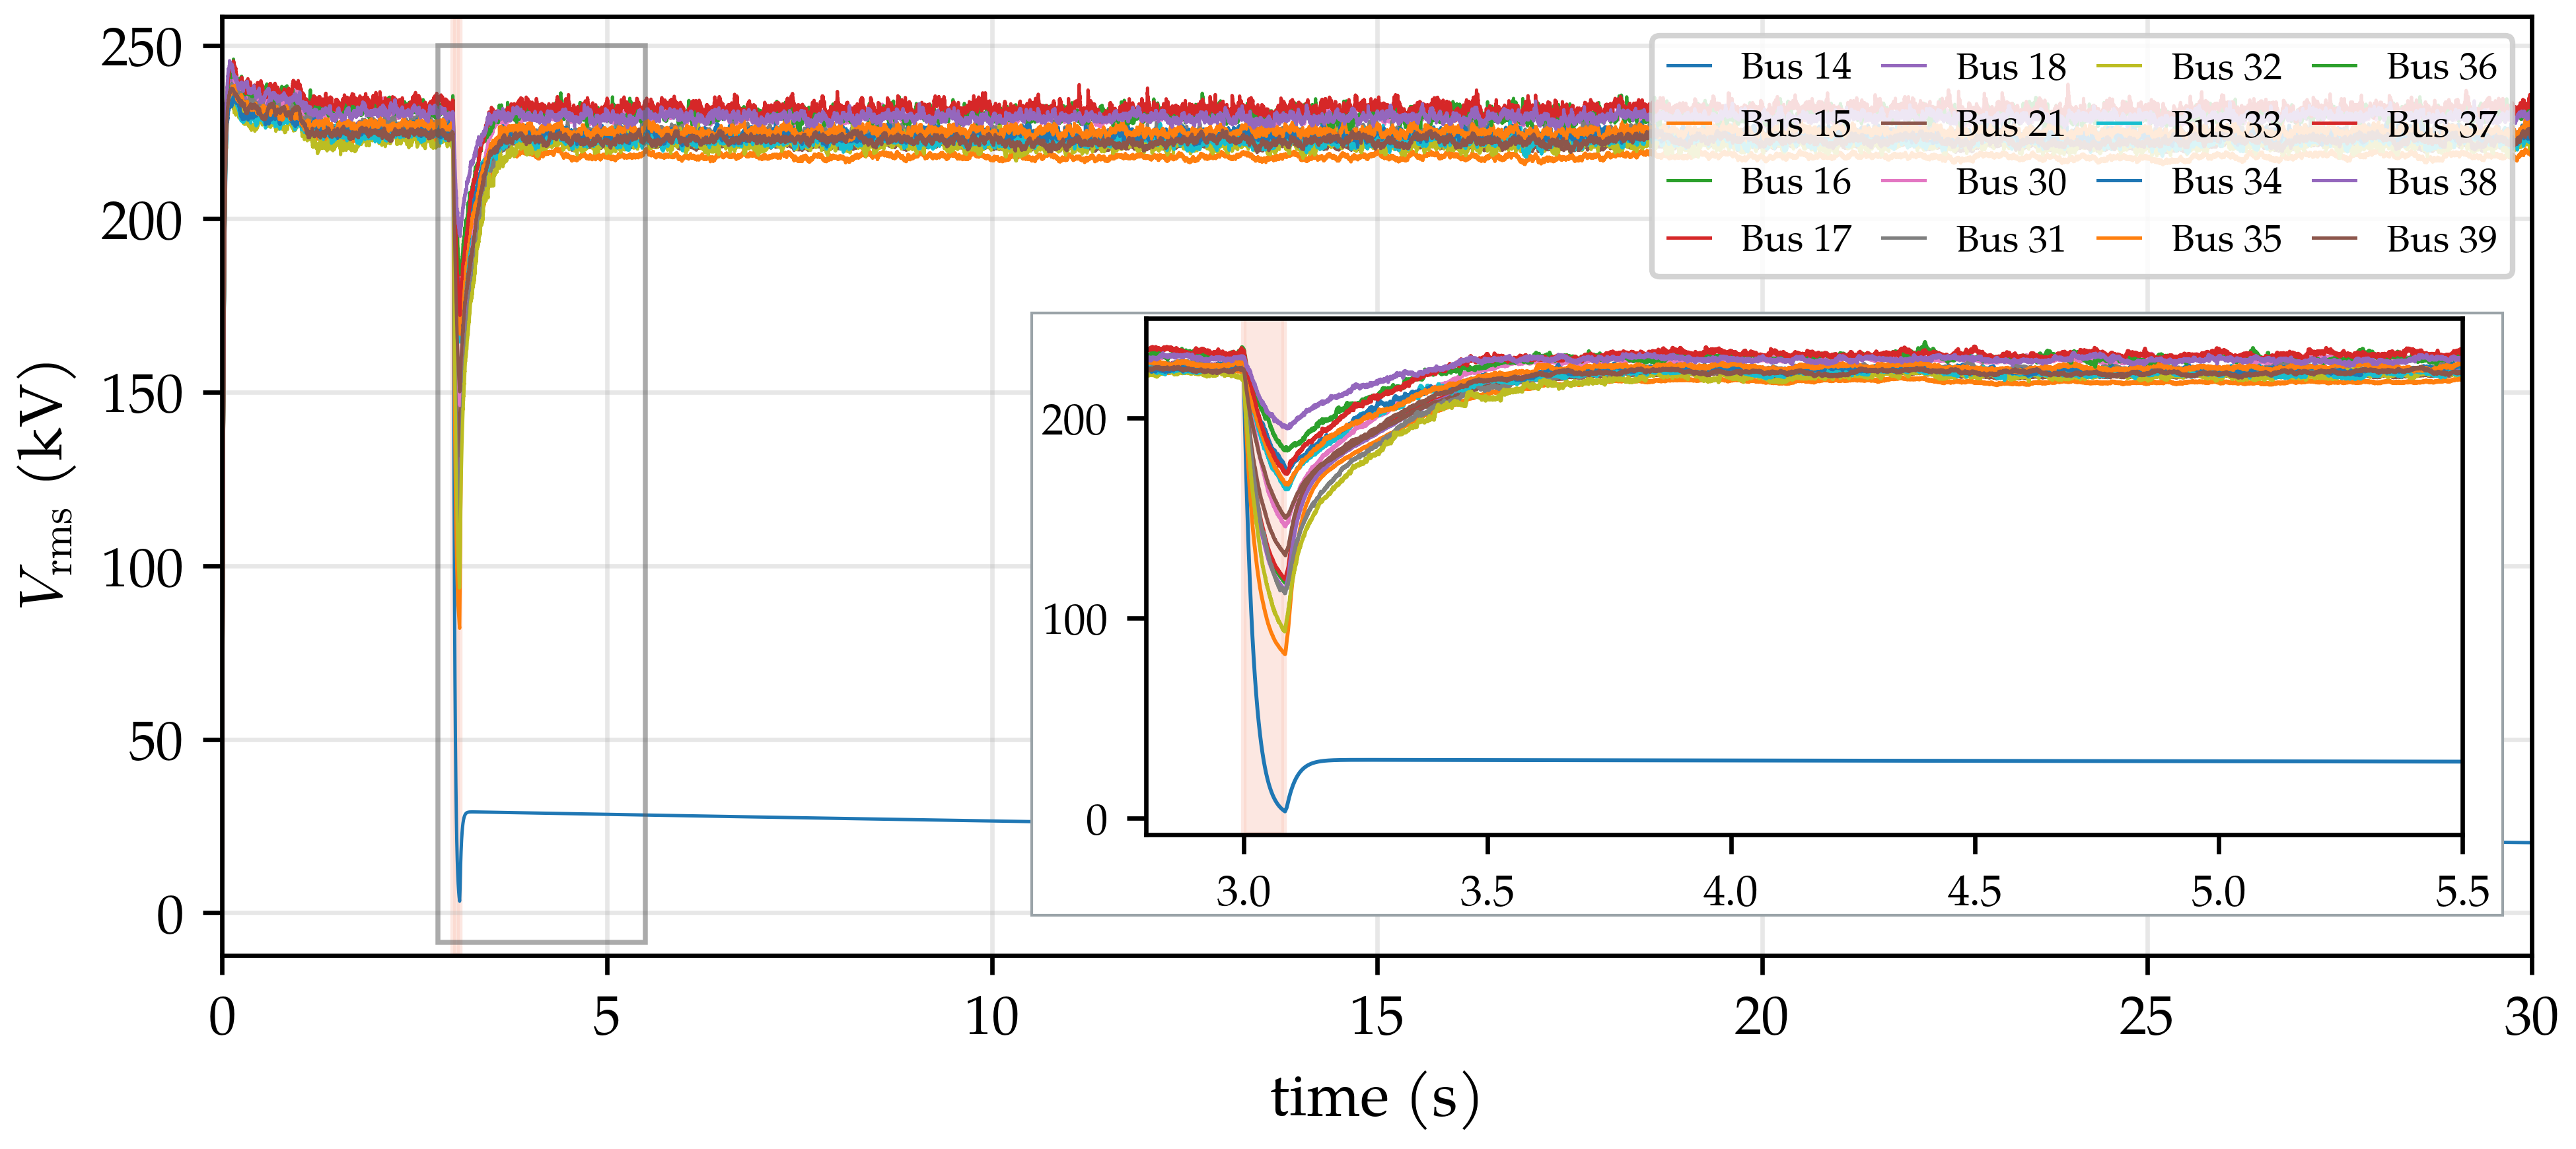
\includegraphics[width=\textwidth]{allgfm_vrms}
\caption{All-GFM bus RMS voltages, in kV, at the monitored network locations under the bus-14 reference fault.}
\label{fig:allgfm}
\end{figure}

\begin{figure}[tbp]\centering
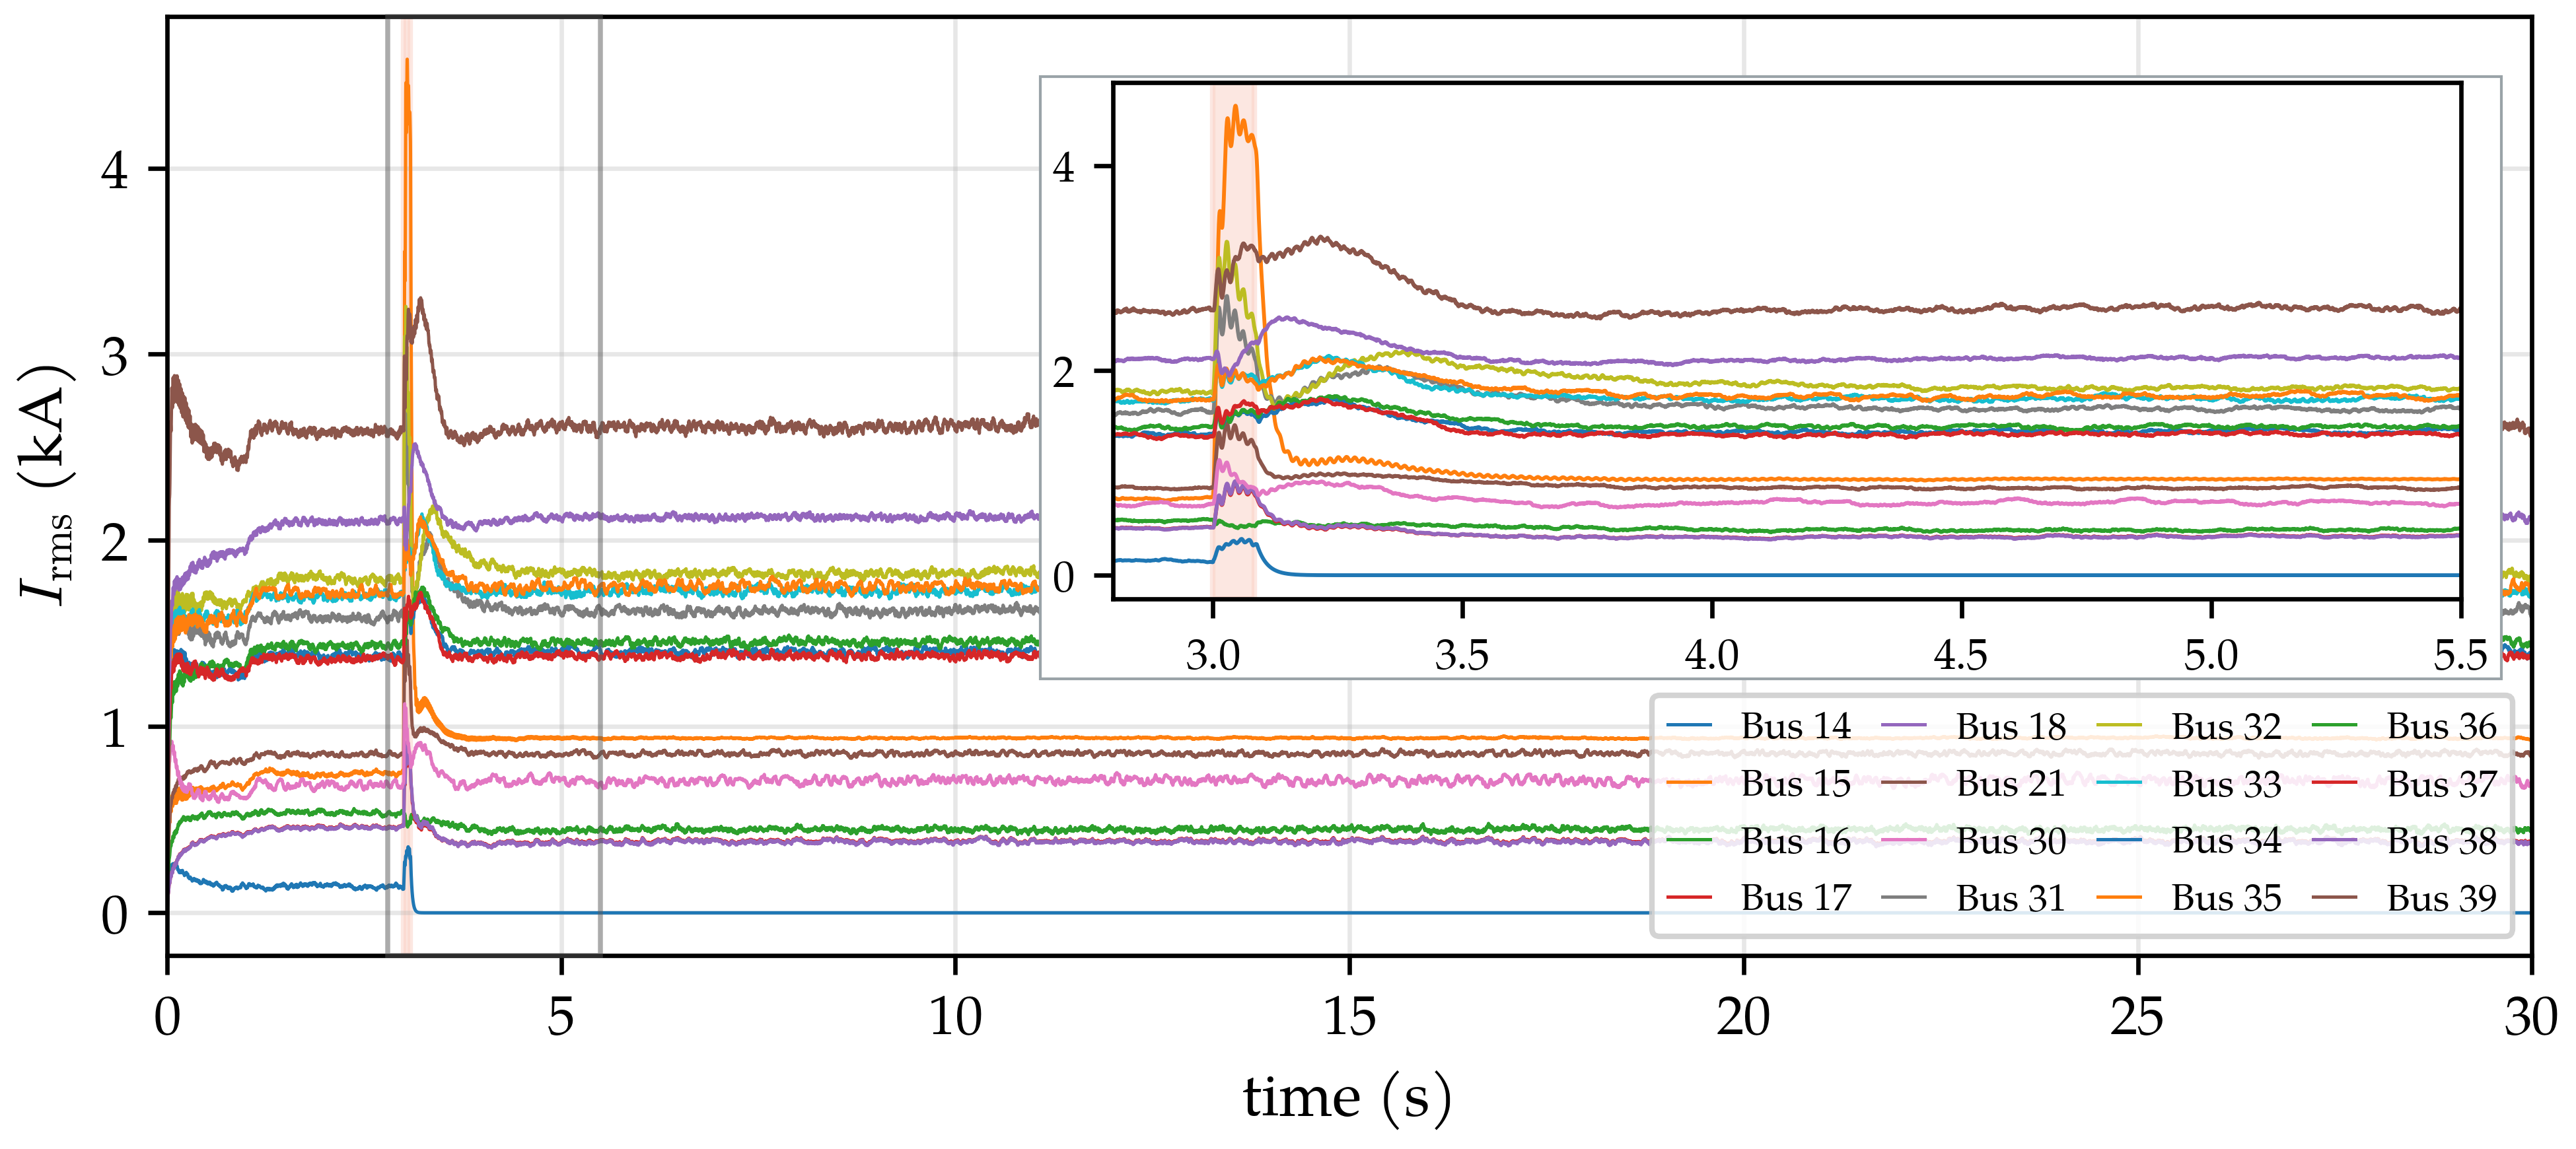
\includegraphics[width=\textwidth]{allgfm_irms}
\caption{All-GFM RMS currents under the bus-14 reference fault, in kA, at the 230~kV meters of network buses 14--18 and~21 and on the 230~kV side of each unit's step-up transformer (buses 30--39), with the transient-current setting $I_{\mathrm{maxF}}=2.0$ per unit on each device base.}
\label{fig:allgfmi}
\end{figure}

\begin{figure}[tbp]\centering
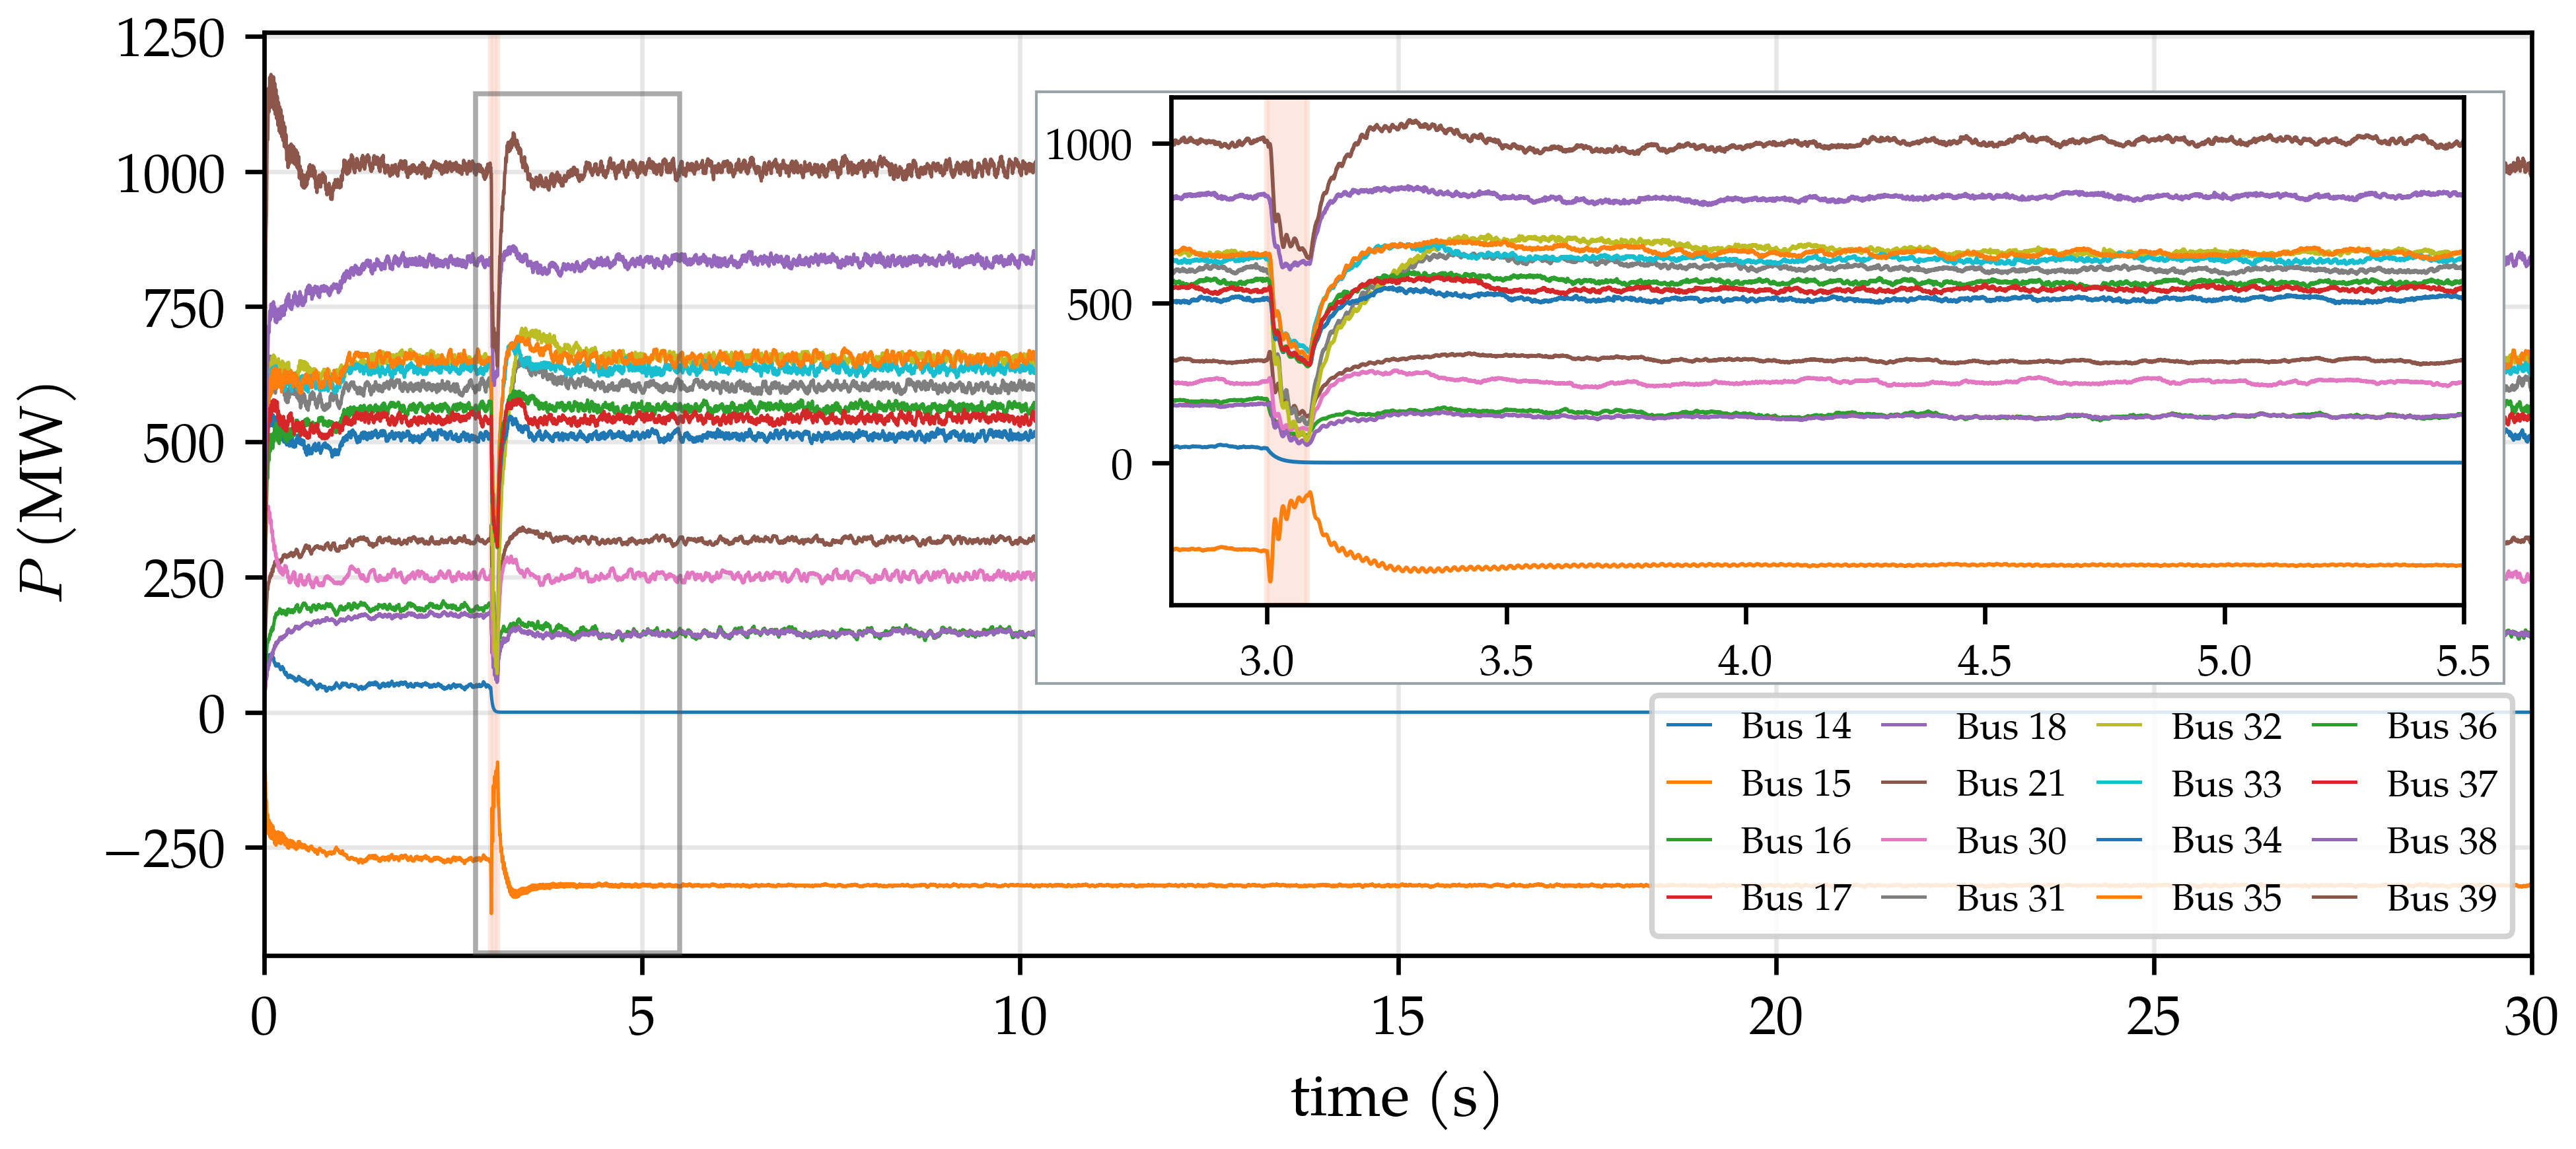
\includegraphics[width=\textwidth]{allgfm_p}
\caption{All-GFM active powers under the bus-14 reference fault, in MW at the meters of Figure~\ref{fig:allgfmi}, signed by the measurement-channel direction.}
\label{fig:allgfmp}
\end{figure}

\begin{figure}[tbp]\centering
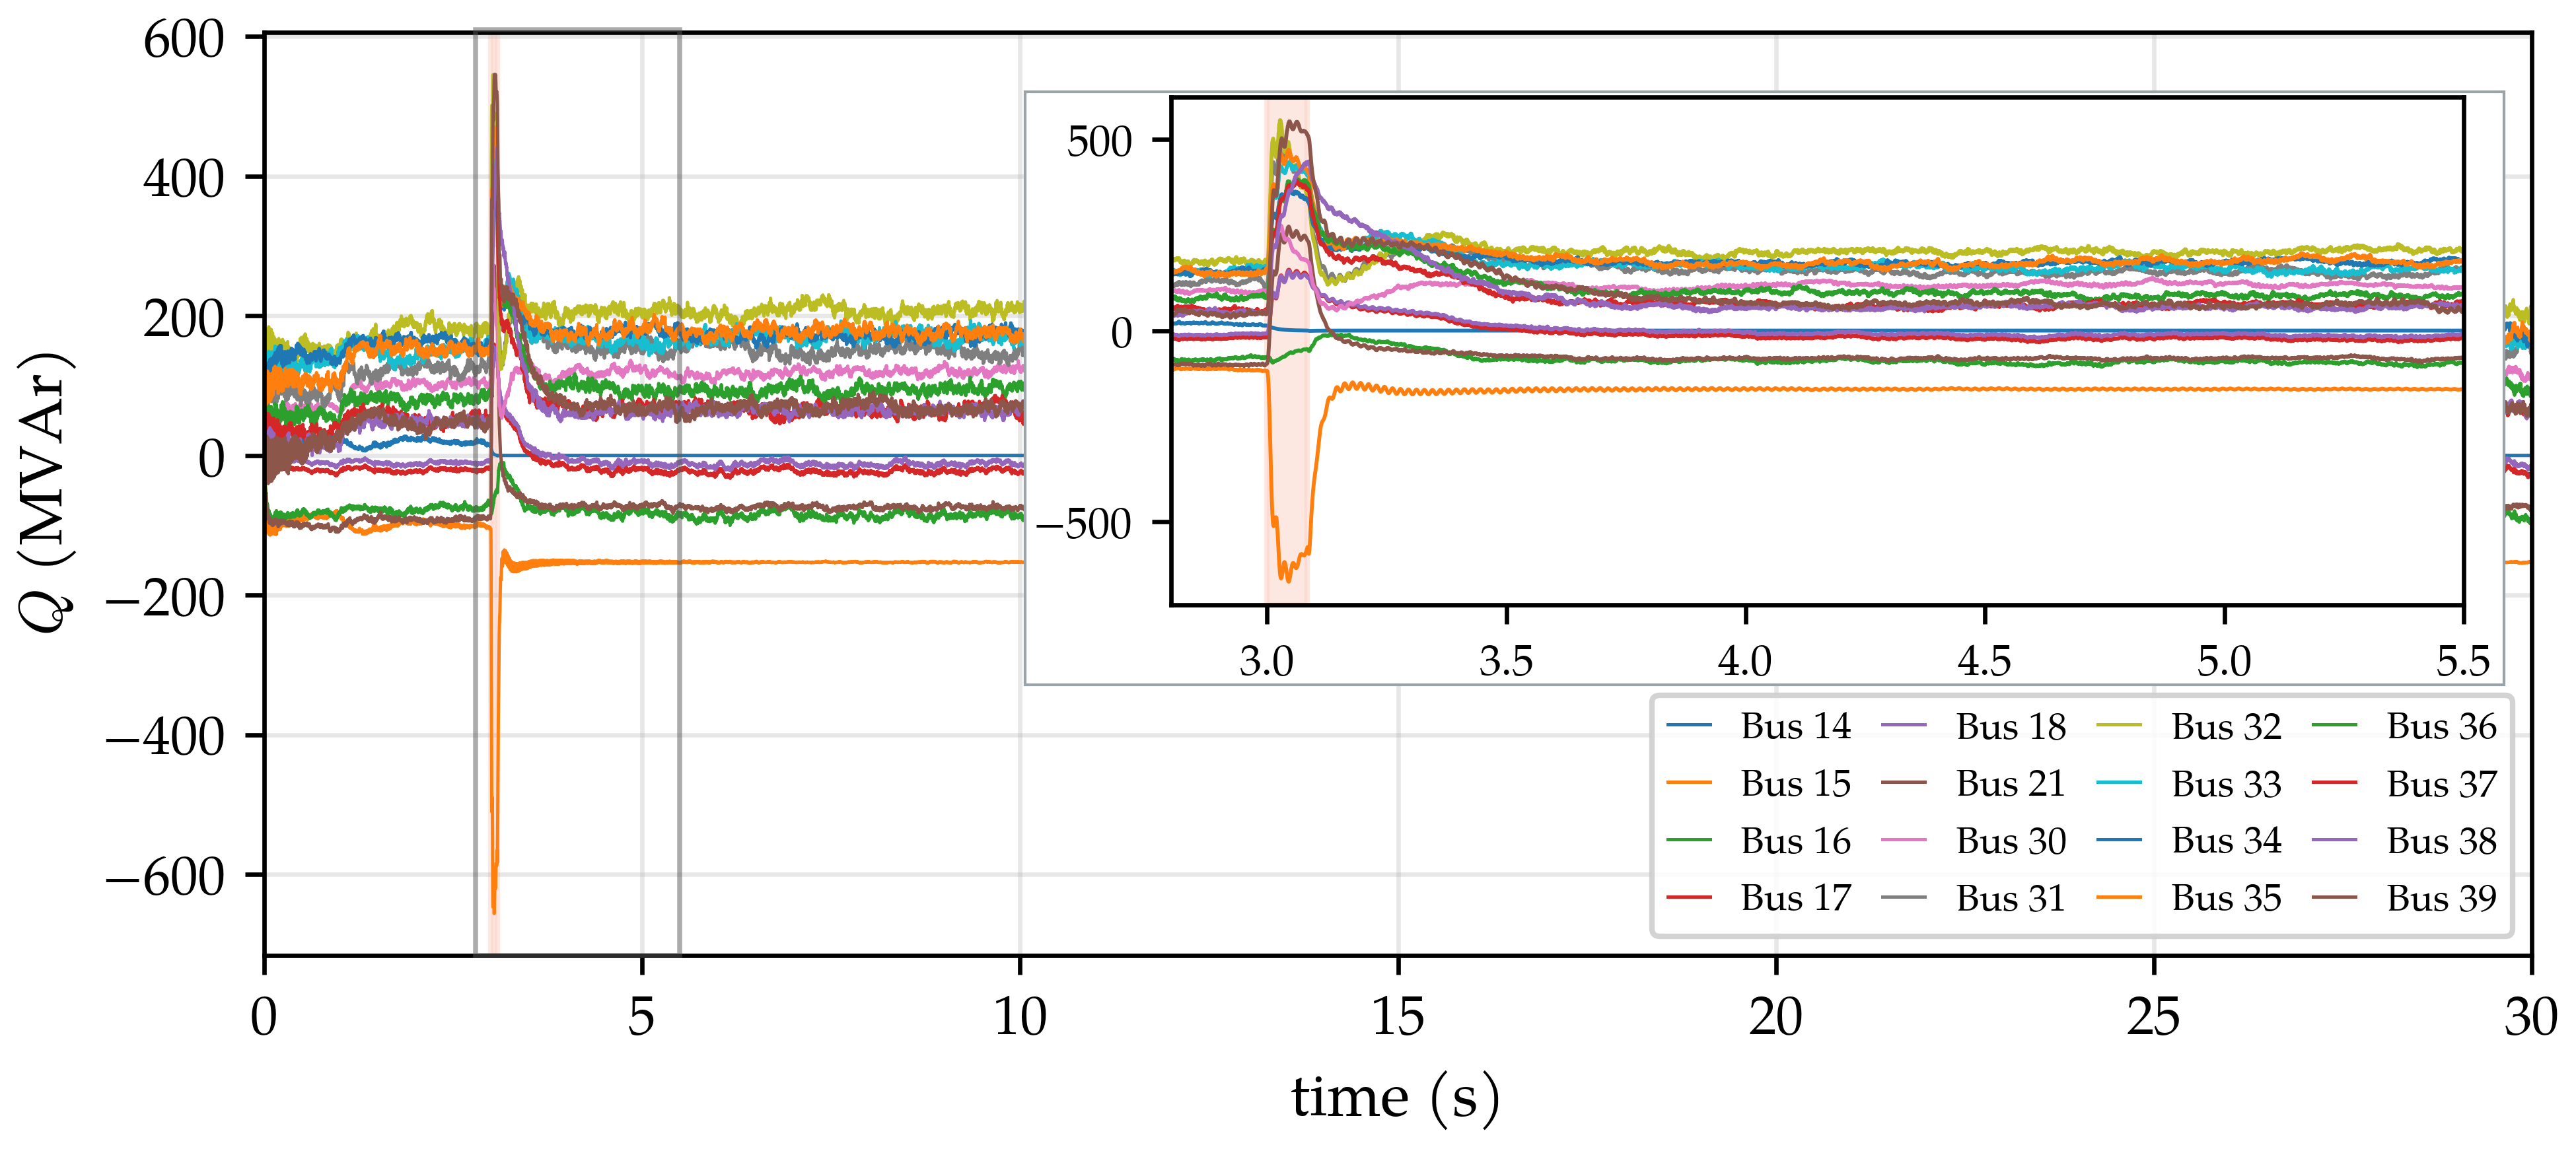
\includegraphics[width=\textwidth]{allgfm_q}
\caption{All-GFM reactive-power responses to the bus-14 reference fault, in MVAr at the meters of Figure~\ref{fig:allgfmi}.}
\label{fig:allgfmq}
\end{figure}

\begin{figure}[tbp]\centering
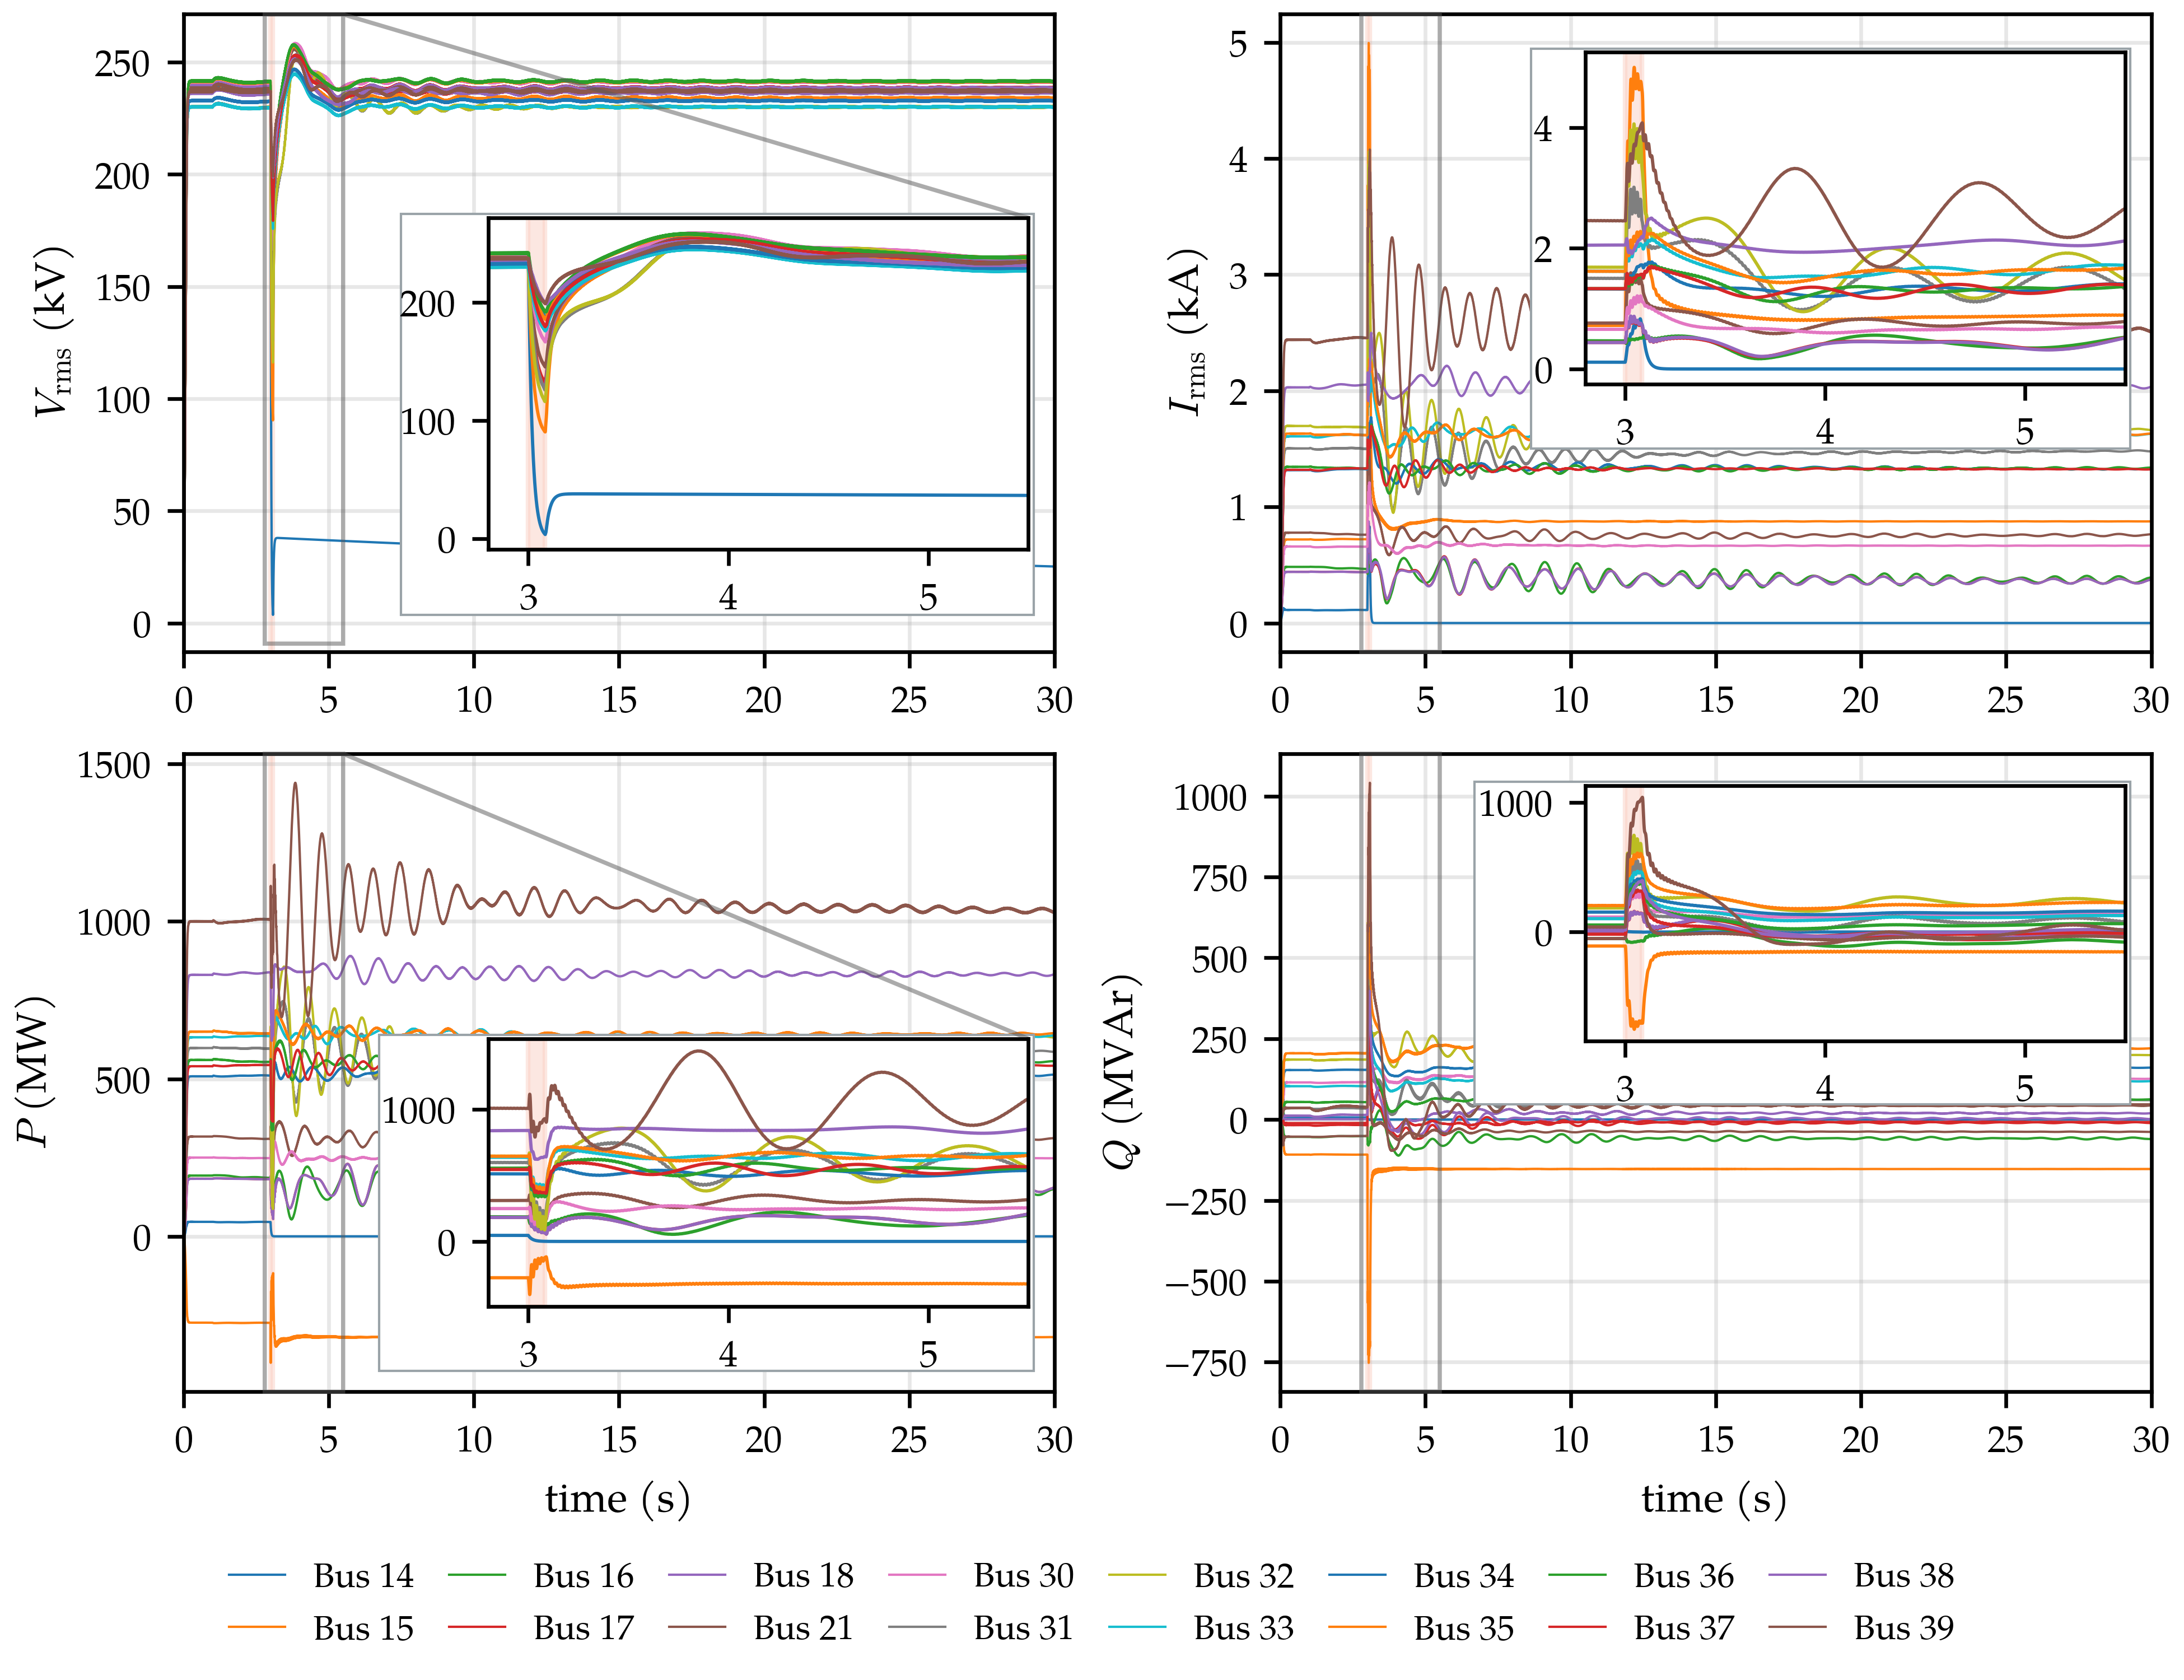
\includegraphics[width=\textwidth]{fig2_allSYNC_3PG_2x2}
\caption{All-machine response to the bus-14 reference fault: RMS voltage and current, active power, and reactive power at network buses 14--18 and~21 and at the 230~kV generator buses 30--39, on the transmission side of the step-up transformers. The active powers oscillate together at about 1~Hz, the inter-machine swing mode, and decay over tens of seconds; bus~14 is isolated by clearing.}
\label{fig:allsync}
\end{figure}

\begin{figure}[tbp]\centering
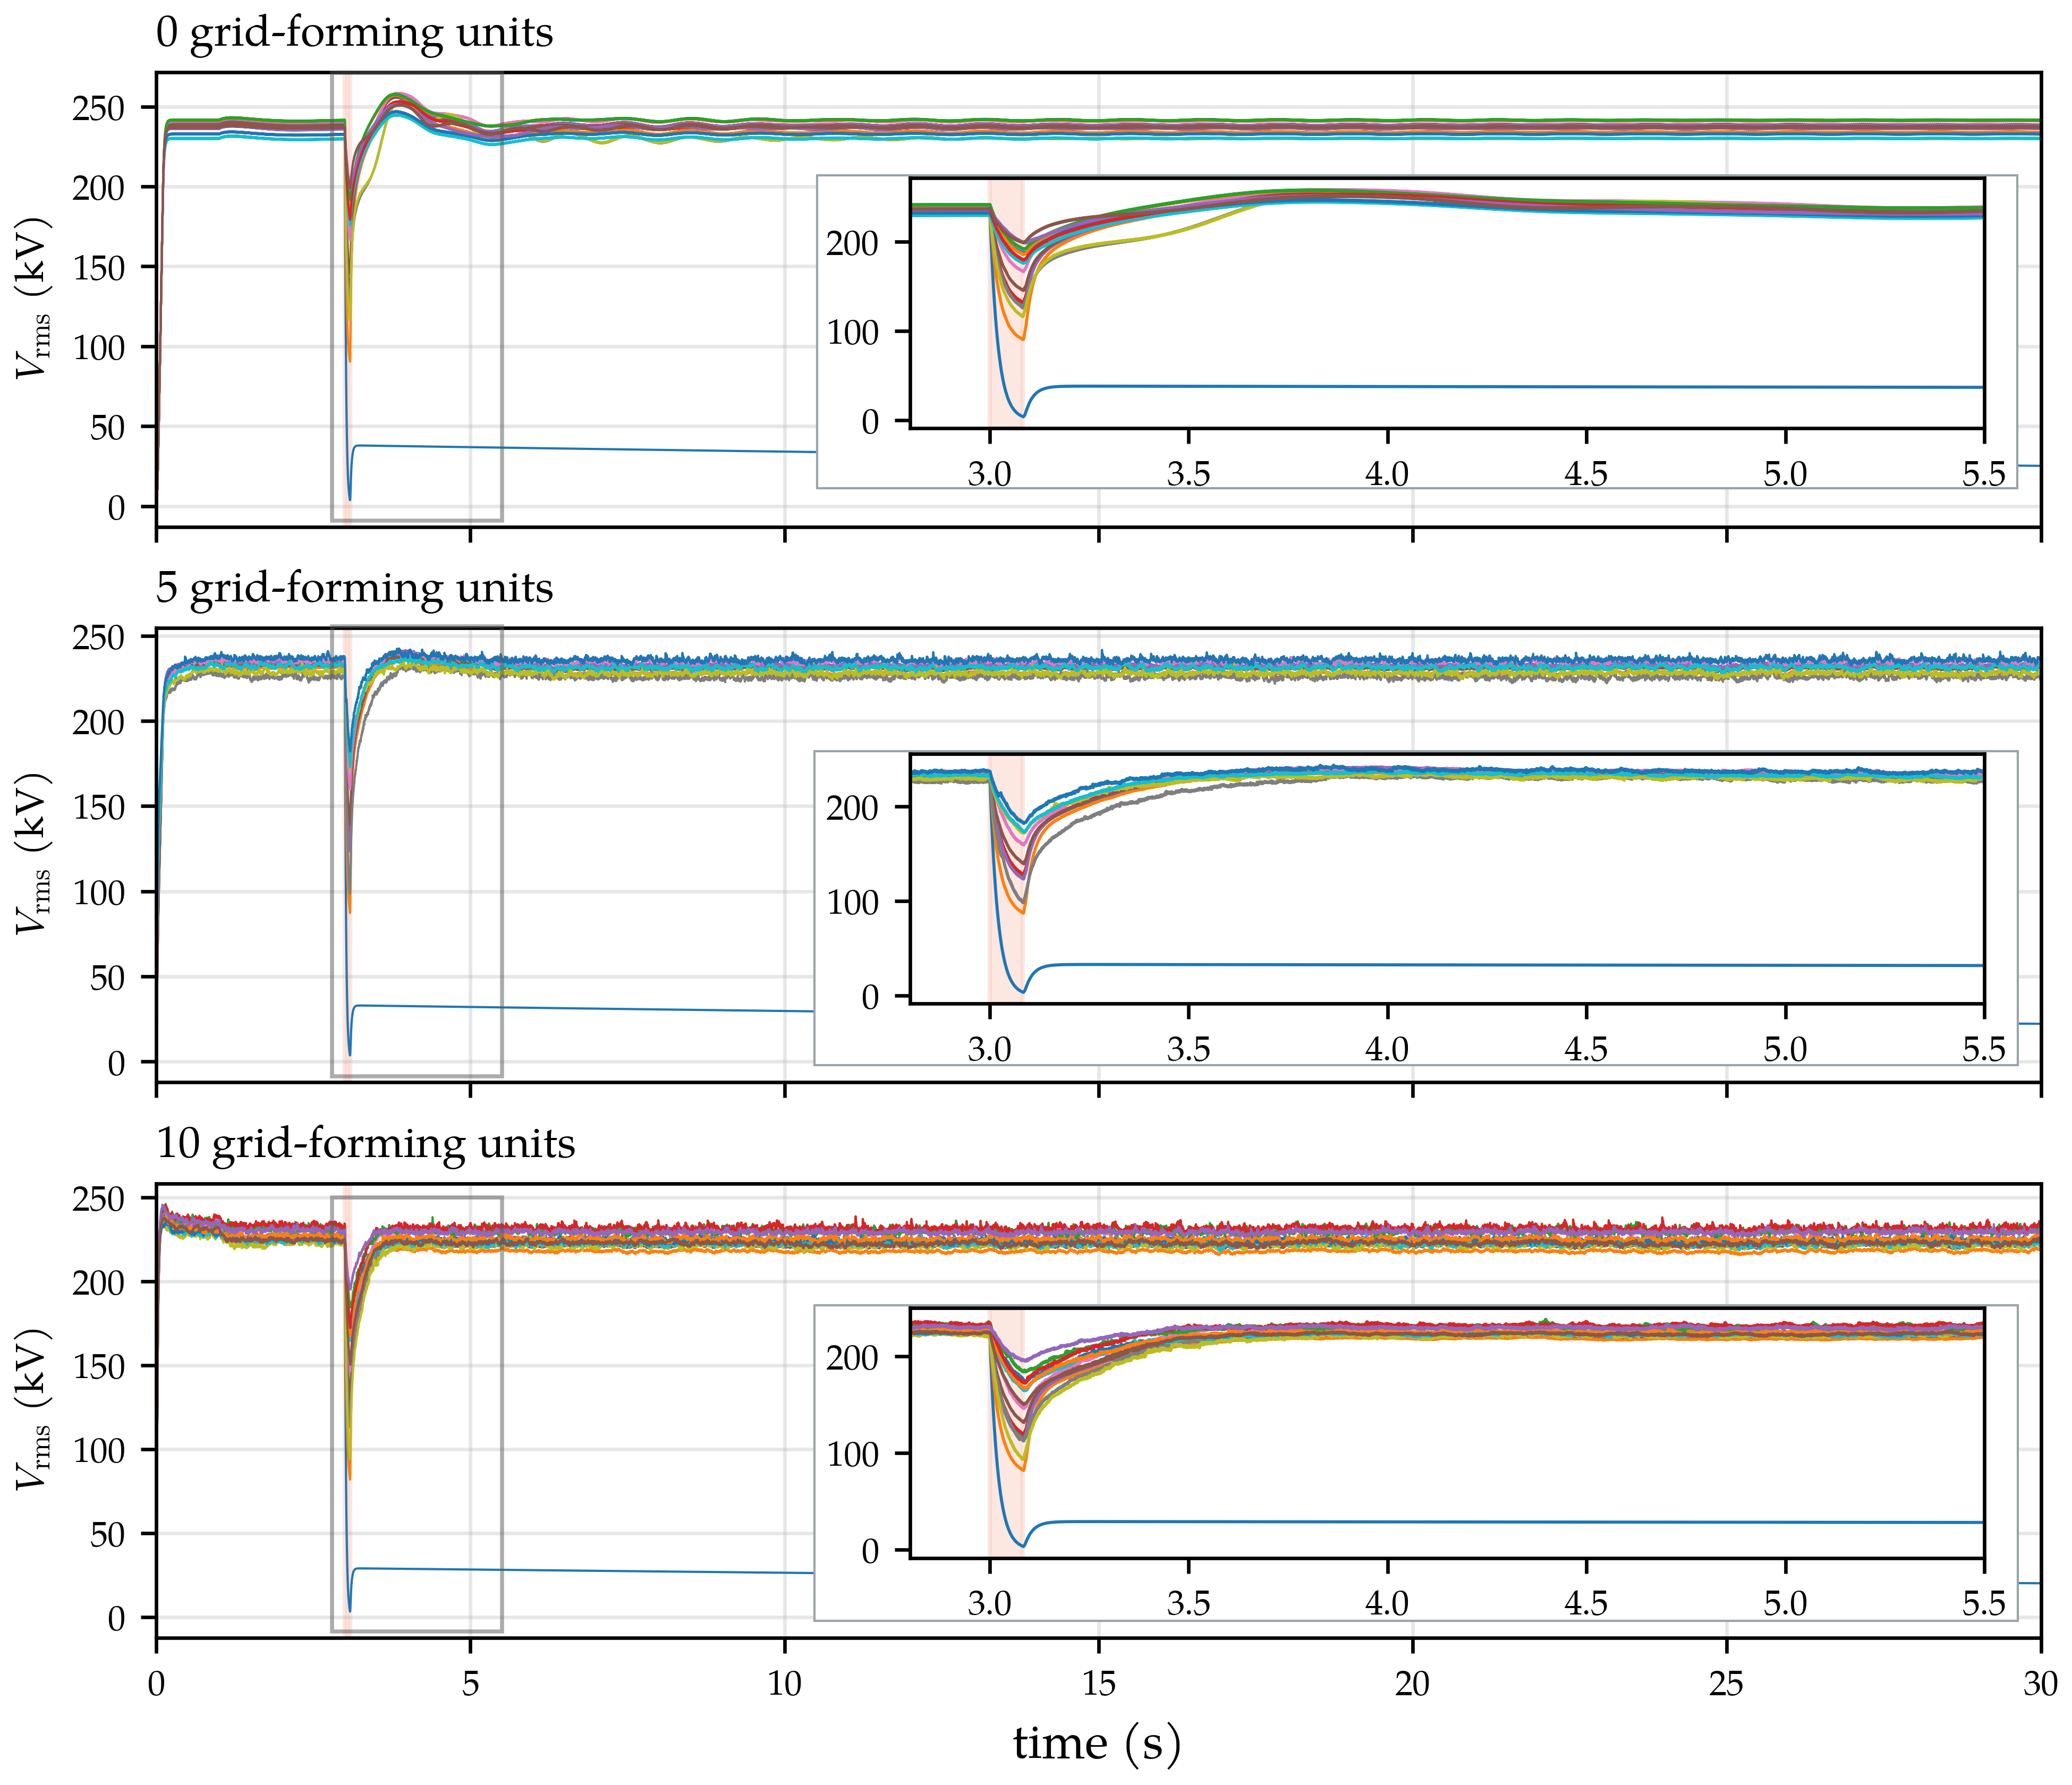
\includegraphics[width=\textwidth]{sweep_0_5_10_GFM_vrms}
\caption{Bus-voltage responses with zero, five, and ten GFM units under the reference fault, with the GFM transient-current setting at 2.0 per unit.}
\label{fig:sweep}
\end{figure}

\subsection{Defining GFM Current-Limiting Behavior}
\label{sec:ilim}
The bus-10 study uses a GFM transient-current setting of 1.5 per unit. Eight units remain at or below that setting, bus~31 reaches the limit, and bus~32 reaches approximately 1.70 per unit, 13\% above the setting, within one cycle of fault inception in the inverter's internal current-magnitude signal, the quantity the limiter compares with $I_{\max F}$. Its terminal RMS current peaks at 1.24 per unit, and its instantaneous phase currents exceed 2.0 per unit of rated peak for at most 3~ms. Figure~\ref{fig:peakits} follows these currents through the full 30~s record. After the transient, the connected units remain below 1.1 per unit and settle near 0.7--0.8 per unit.

The bus-32 current falls to zero after clearing, while the other nine units continue carrying current. The case associates this loss of output with opening the bus-10 network connections without reclosing. Continued network recovery therefore does not mean that the zero-current resource continues exporting power. This distinction is important when interpreting the fleet response after a clearing action.

\begin{figure}[tbp]\centering
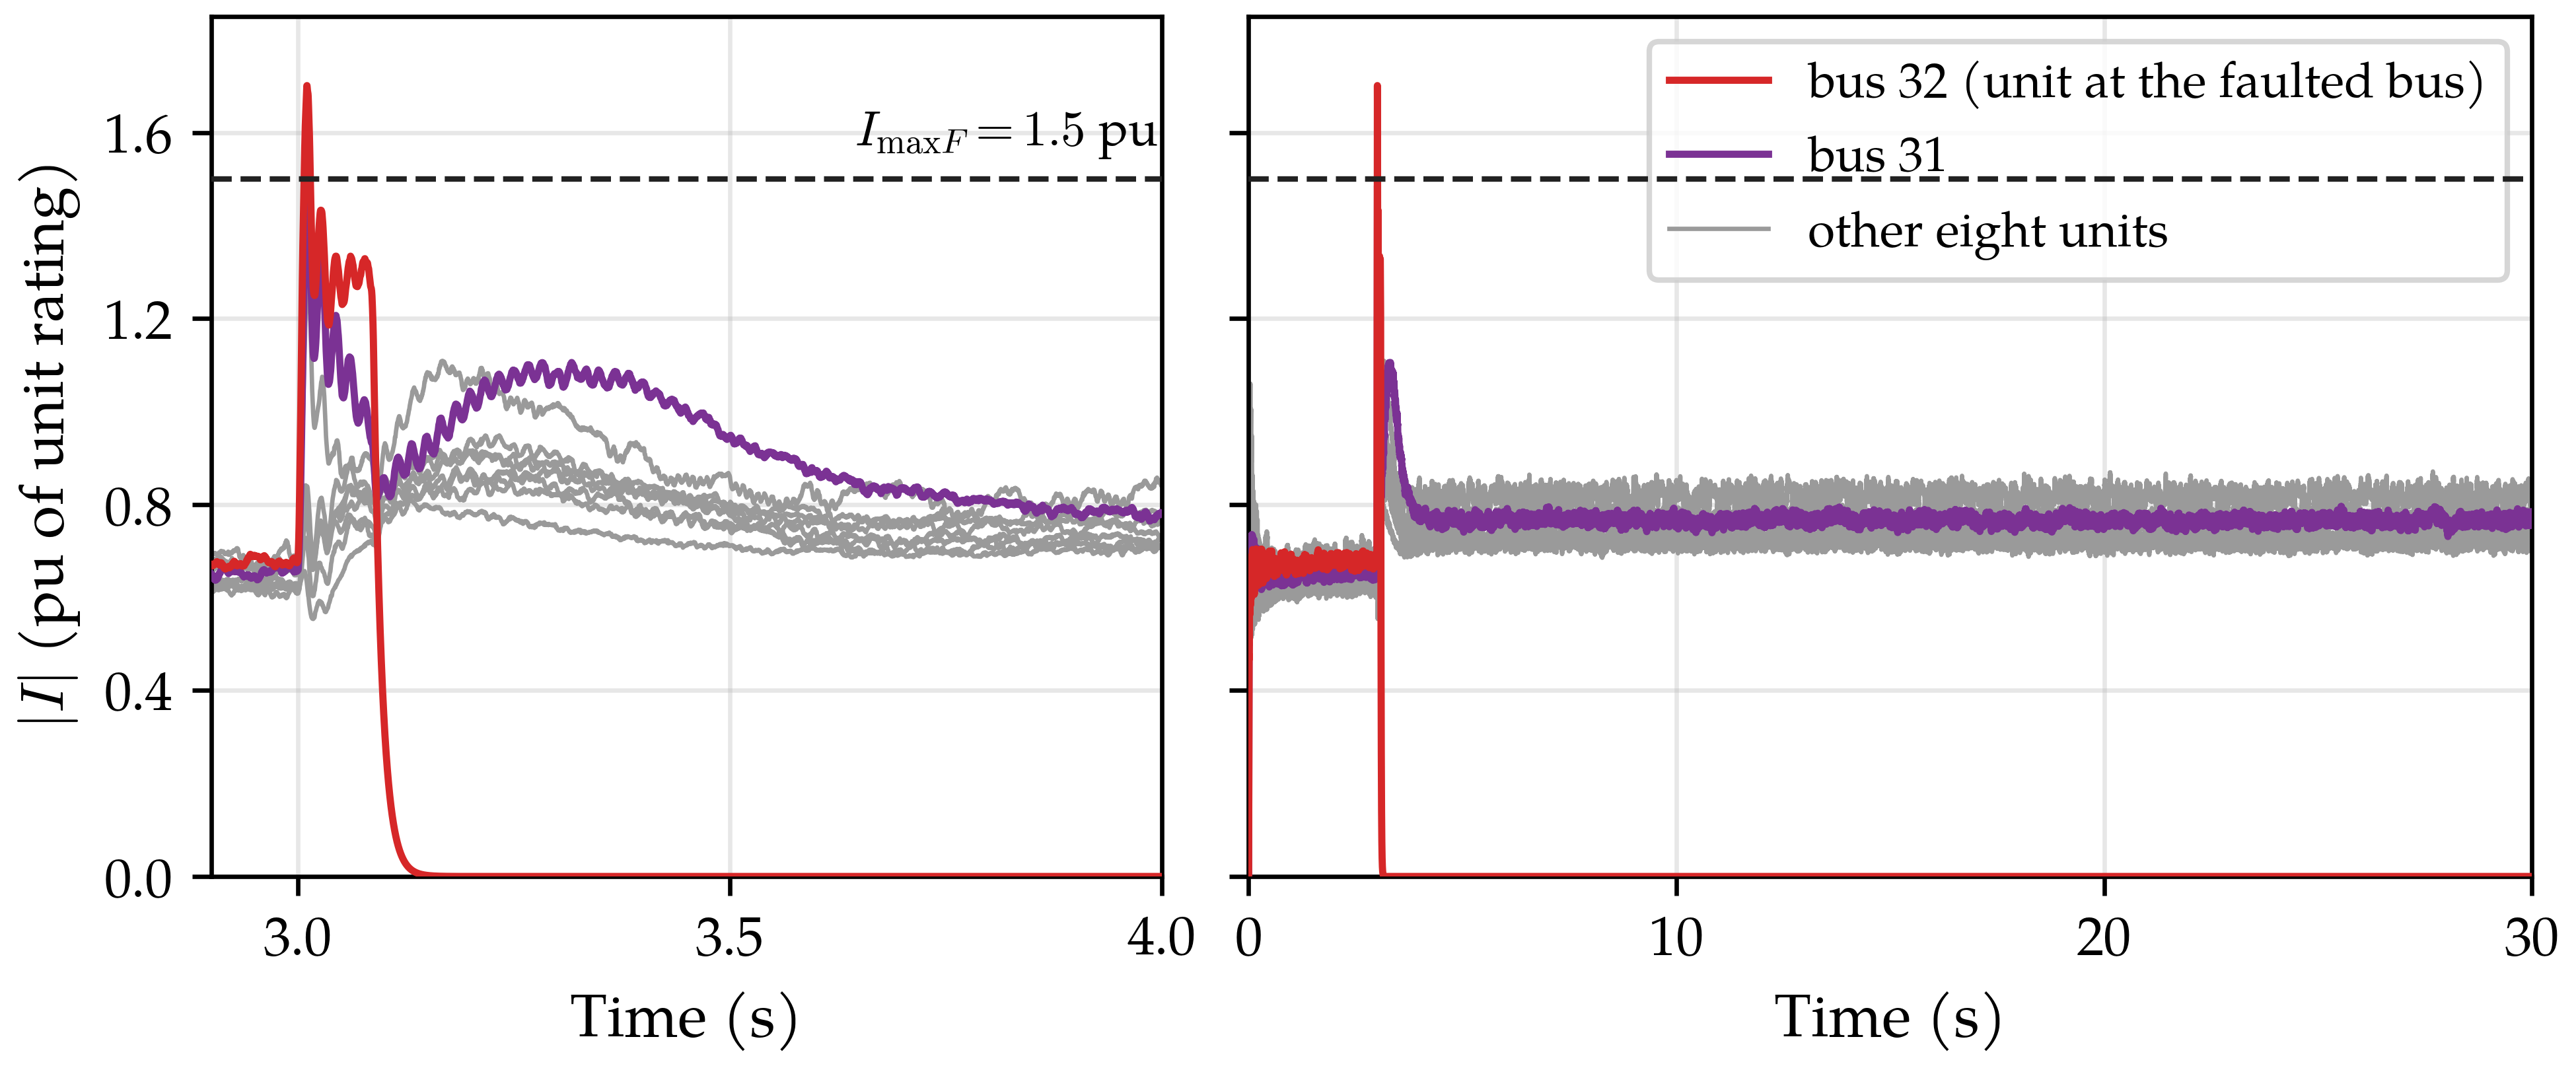
\includegraphics[width=\textwidth]{narr_peakI_timeseries}
\caption{Bus-10 current-limit study with a five-cycle fault and no reclosing: each trace is the inverter's own current magnitude at its terminals, on the 10~kV side of its step-up transformer, in per unit of the unit rating. With a 1.5 per-unit setting, bus~32 reaches approximately 1.70 per unit before falling to zero; nine units continue carrying current.}
\label{fig:peakits}
\end{figure}

Figure~\ref{fig:ilimarms} compares the bus-14 reference fault on the all-GFM fleet at $I_{\max F}=2.0$, 1.5, 1.2, and 1.1 per unit with all other settings unchanged; the last two are sensitivity points well below the 2.0 per-unit default. The fault is electrically remote from the units: at 2.0 per unit no unit reaches its limit, with peaks of 1.53, 1.44, and 1.38 per unit at buses~32, 30, and~31 and the other seven below 0.92 per unit. At 1.5 per unit only the bus-32 unit touches the limit, for 1.4~ms. At 1.2 per unit the three nearest units exceed the limit in the internal current-magnitude signal, with peaks of 1.44, 1.38, and 1.31 per unit at buses~32, 30, and~31; the limiter returns the current to the limit within half a cycle at buses~30 and~31 and within 1.7 cycles at bus~32, whose current makes a second, smaller excursion, so the total time above the limit is 0.4 to 0.8 cycle. At 1.1 per unit the same three units peak at 1.43, 1.30, and 1.28 per unit and are back at the limit after 1.8, 0.9, and 0.9 cycles; unit~32's current averages 0.94 per unit over the third to fifth cycles of the fault, against 1.05 at 2.0 per unit. Instantaneous failures of the semiconductor switches, which occur on a much faster timescale than the limiter's correction, are not modeled: the units stay connected and the control limiter alone bounds the current. In all four cases every unit rides through: post-fault active power returns to within 0.5\% of its pre-fault value and the frequency settles at 60.01~Hz.

\begin{figure}[tbp]\centering
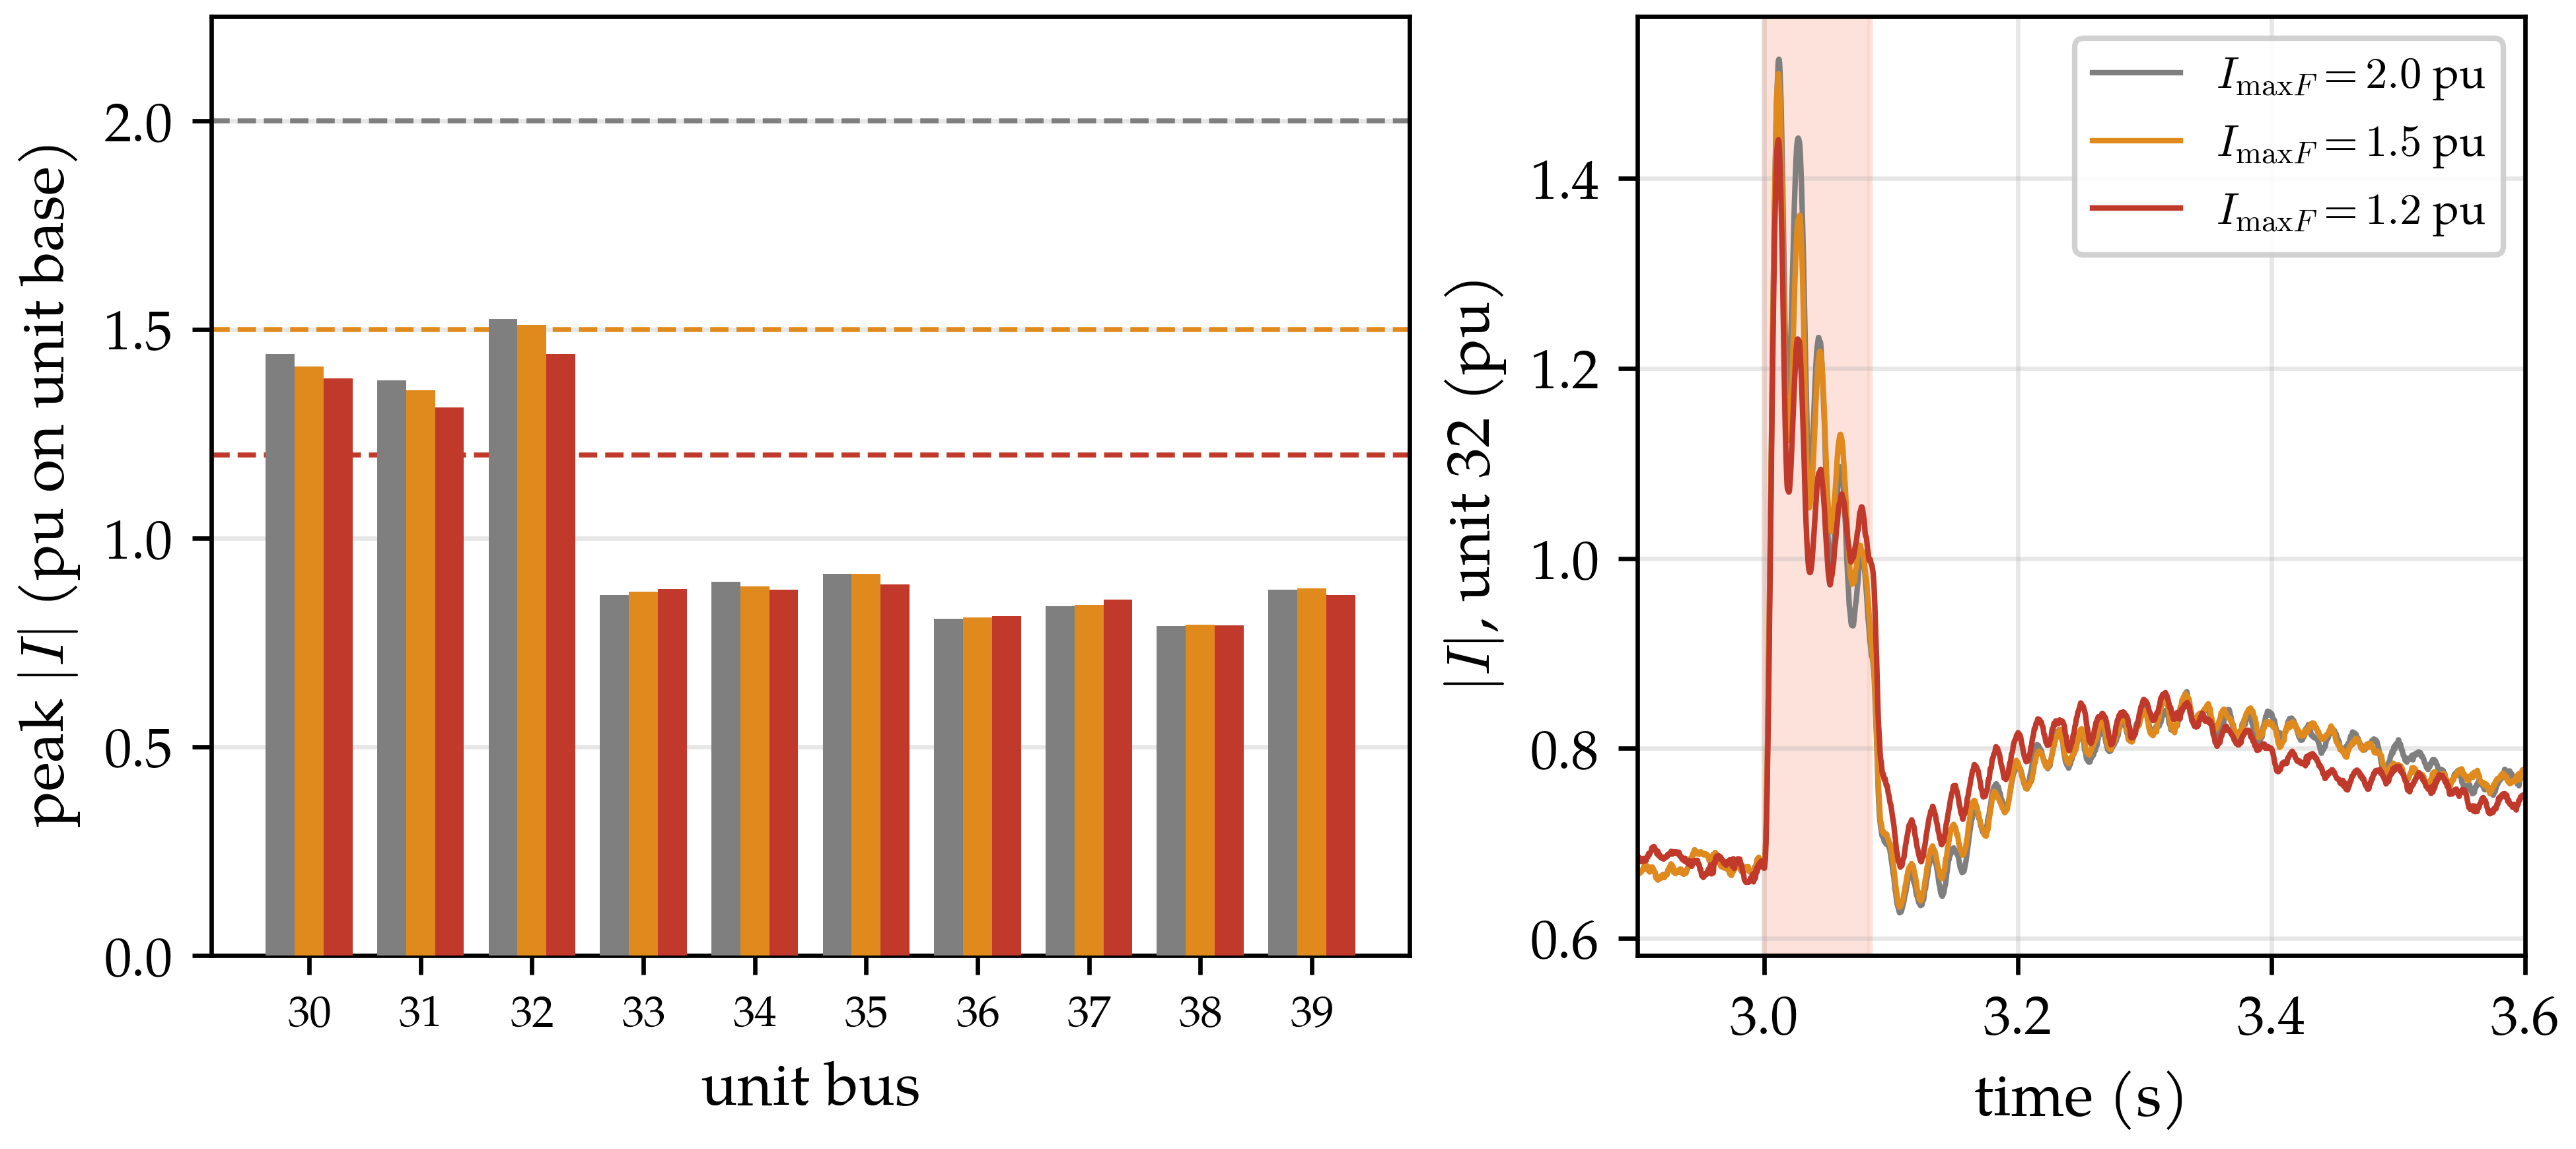
\includegraphics[width=\textwidth]{narr_ilim_arms_bus14}
\caption{Bus-14 reference fault on the all-GFM fleet at four transient current limits, 10~s records with identical dispatch, fault, and clearing. Left: peak of each unit's internal current magnitude (10~kV side of the step-up transformer) on its own base, with the limit lines; right: the same signal for the bus-32 unit through the fault. Instantaneous failures of the semiconductor switches are not modeled.}
\label{fig:ilimarms}
\end{figure}

Because the bus-14 fault is remote, Figure~\ref{fig:ilimarms13} repeats the comparison with the fault at bus~13, one short line from bus~10, the point of interconnection of unit~32, and adds an arm with the limit raised to 15 per unit, beyond any current the network can deliver. Clearing opens lines 10--13 and 13--14, and unit~32 stays connected through line 10--11. Without a practical limit the unit-32 current peaks at 1.83 per unit and the units at buses~31 and~30 at 1.43 and 1.30, so the 2.0 per-unit default is not reached even one line from the unit's point of interconnection. With the default settings the first peak is 1.69 per unit; the difference from the unlimited arm comes almost entirely from the model's hard clip on the instantaneous current at 2.1 per unit acting on the sub-cycle transient (a run with the limit at 15 and the clip at 2.1 peaks at 1.72), not from the 2.0 per-unit limiting function. Figure~\ref{fig:ilimarms13}(c) shows how quickly the limits take hold: the traces rise together for the first 5~ms, then separate, and the 1.5 per-unit limit holds unit~32 after an overshoot to 1.63 per unit that lasts 0.4 cycle, back at the limit 14~ms (0.8 cycle) after inception. The 1.2 per-unit limit holds the three nearest units after overshoots to 1.59, 1.35, and 1.28 per unit; unit~32 makes a second, smaller excursion and is back at the limit after 1.7 cycles, the other two after 0.8 cycle. The 1.1 per-unit limit holds them after overshoots to 1.59, 1.31, and 1.24 per unit, back at the limit after 1.8, 0.9, and 0.9 cycles. After the first two cycles the fault-on current of unit~32 settles at 1.16 to 1.21 per unit in the three arms at 1.5 per unit and above, so those limits act on the initial transient only; the 1.2 and 1.1 per-unit limits hold it at 1.04 and 0.98 per unit for the rest of the fault. Every unit rides through in these five arms: post-fault active power returns to within 0.3\% of its pre-fault value and the frequency settles at 60.01~Hz. A sixth run at 1.0 per unit, a limit at rated current, does not recover (Figure~\ref{fig:ilimarms13}(e)). Its pre-fault state and first cycles match the other arms (unit-32 peak 1.44 per unit, back at the limit after 1.8 cycles), but half a second after fault inception the 230~kV voltages at the unit buses are 0.68 to 0.84 per unit, against 1.00 to 1.06 at 1.1 per unit, and they keep falling; from 7.0~s the units at buses~31, 32, and~39 leave synchronism, with droop-frequency excursions up to 1.3~Hz and intervals of negative power, and at the end of the record the fleet delivers 3465~MW of the 6252~MW it supplied before the fault. The unit currents after clearing are mostly below the limit, between 0.6 and 0.9 per unit, so the limit does not bind continuously: the fleet does not obtain the current that the voltage recovery needs in the first instants after clearing and settles on a low-voltage operating point. For this fault the smallest limit that rides through therefore lies between 1.0 and 1.1 per unit.

\begin{figure}[tbp]\centering
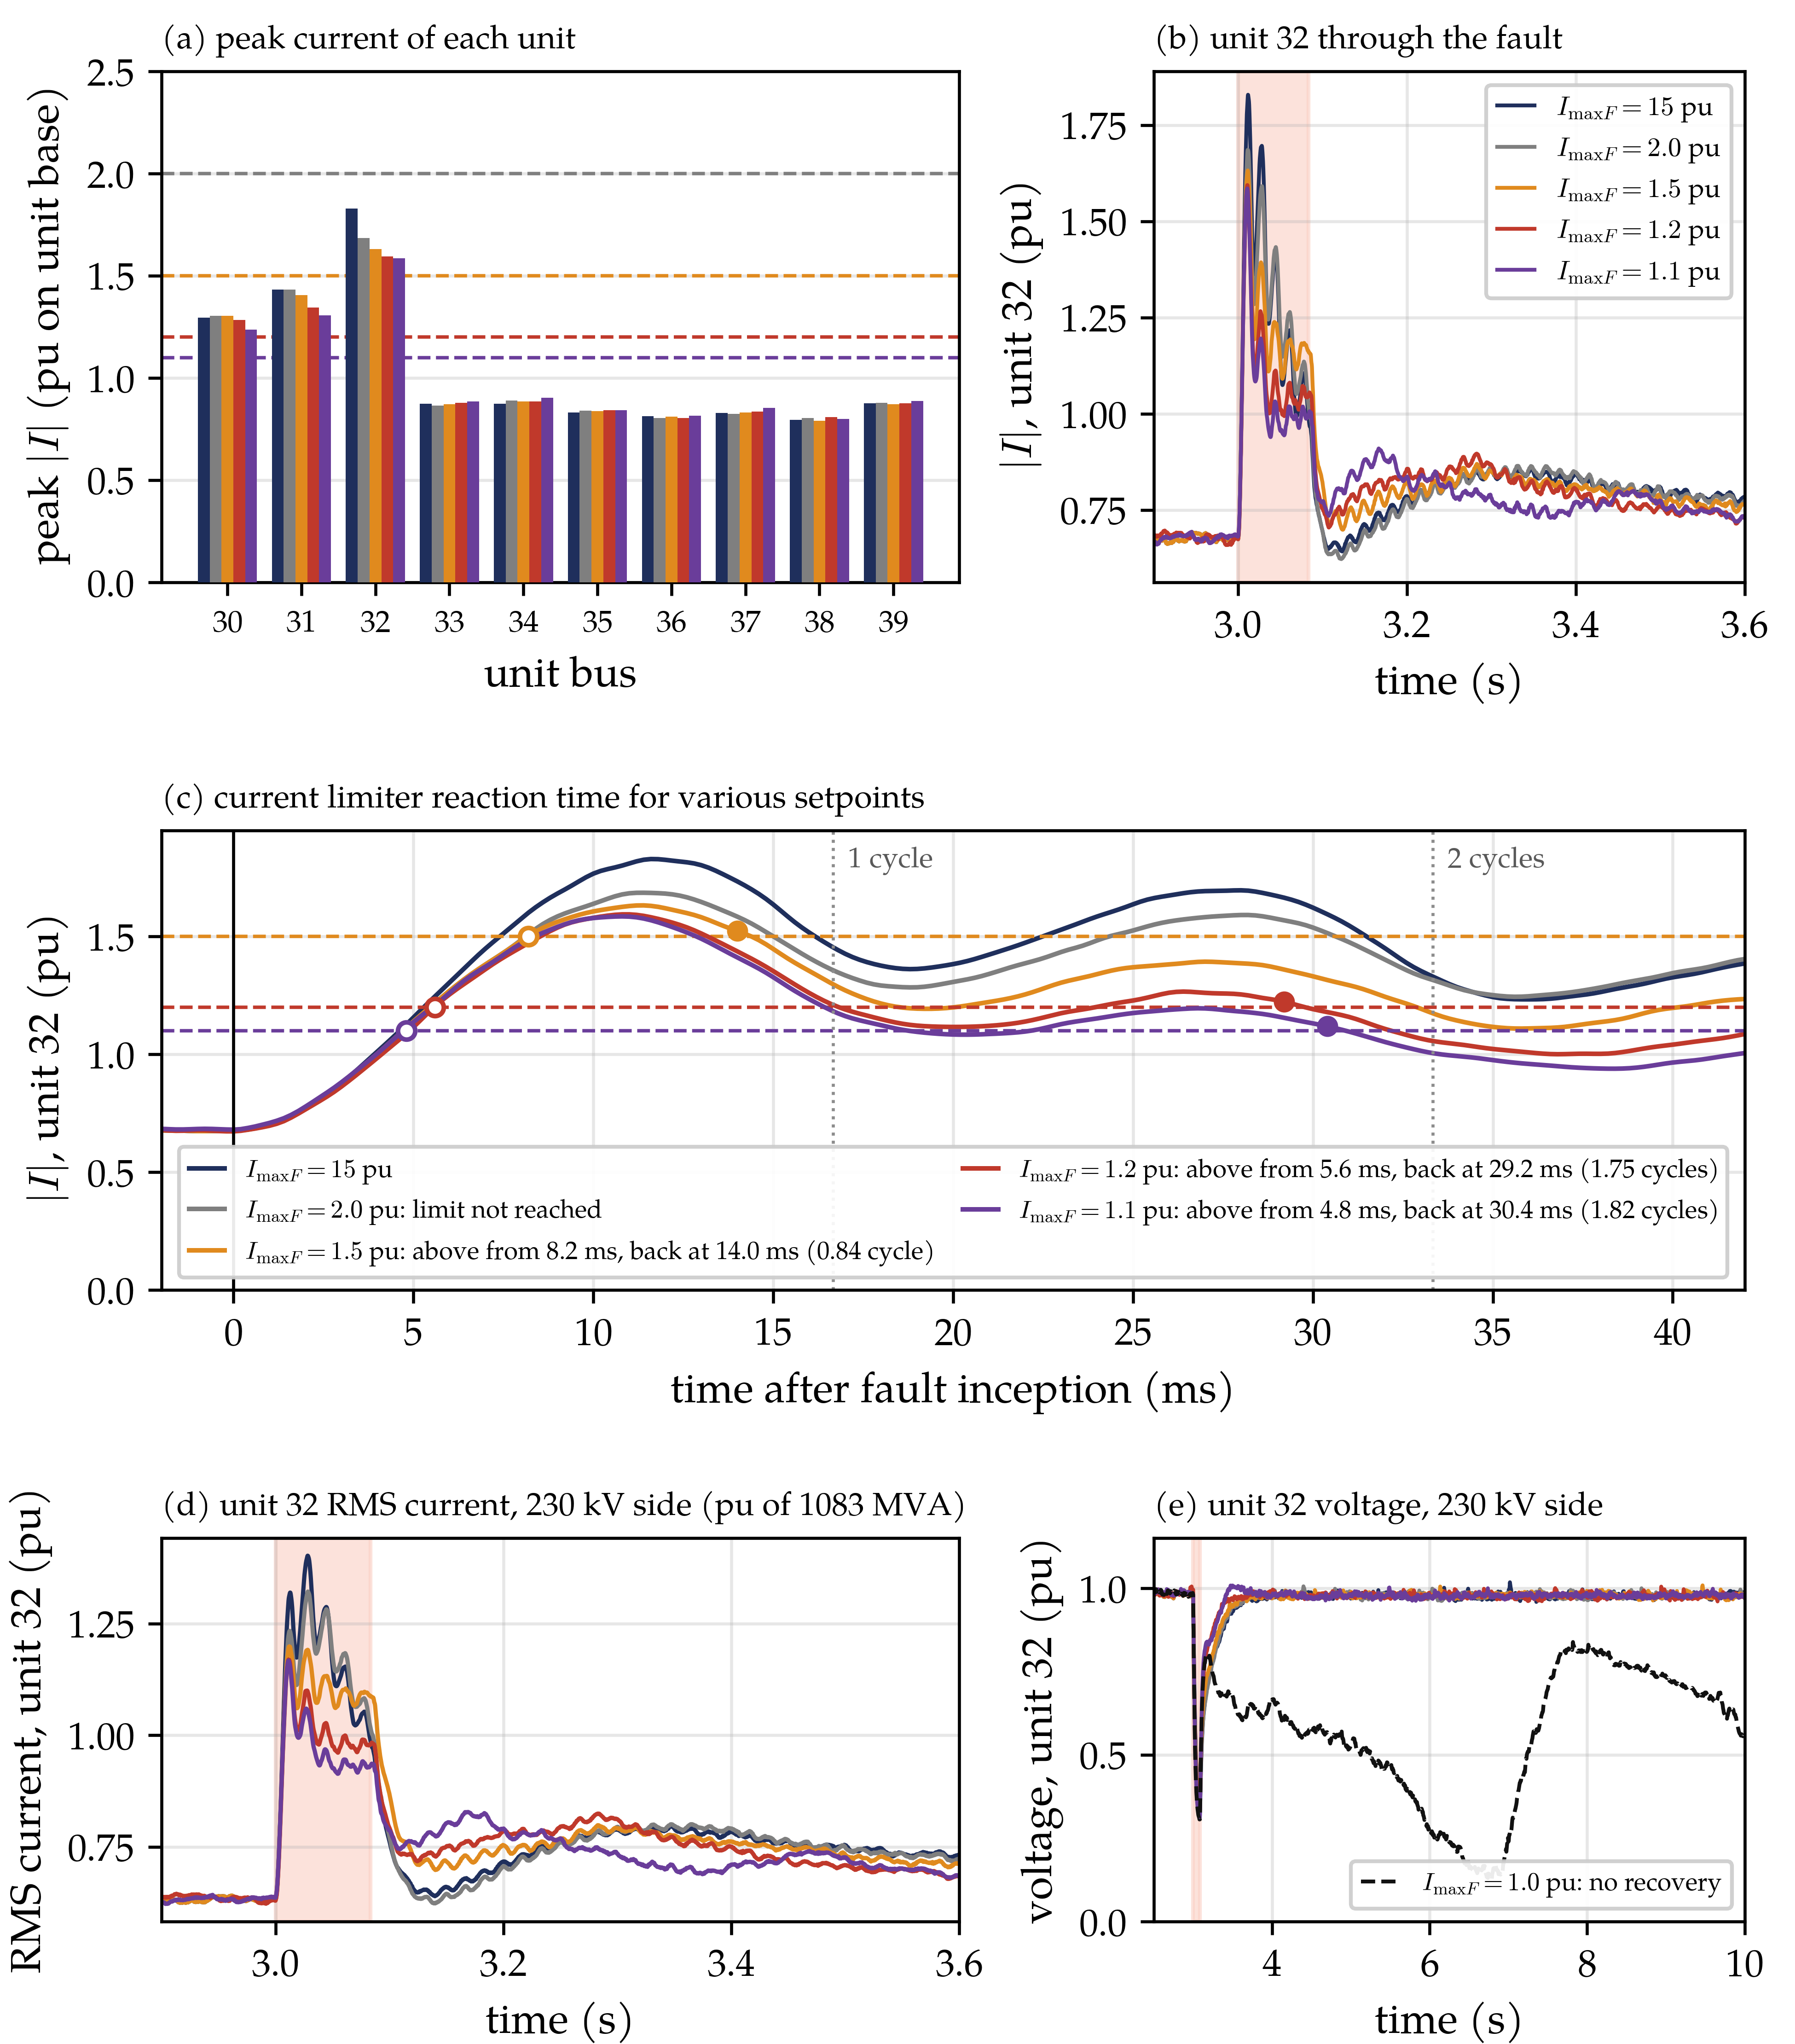
\includegraphics[width=\textwidth]{narr_ilim_arms_bus13}
\caption{Bus-13 fault on the all-GFM fleet at five transient current limits (the 15 per-unit arm has no practical limit), 10~s records with identical dispatch, fault, and clearing, which opens lines 10--13 and 13--14. (a)~Peak of each unit's internal current magnitude (10~kV side of the step-up transformer) on its own base, with the limit lines. (b)~The same signal for the bus-32 unit through the fault. (c)~The first two and a half cycles: for each setpoint the legend gives when the current first exceeds the limit (open circle) and when it is back within 2\% of it and held for a cycle (filled circle). (d)~RMS current of the bus-32 unit on the 230~kV side of its step-up transformer, in per unit of the unit rating (1083~MVA, 2.72~kA). (e)~Voltage of the bus-32 unit on the 230~kV side over the whole record, with a sixth run at 1.0 per unit (dashed), which does not recover.}
\label{fig:ilimarms13}
\end{figure}

Figure~\ref{fig:peaki} compares the device-base peak currents, including a machine peak of 3.72 per unit at the corresponding bus. GFM current is shaped by the modeled current limit, whereas machine fault current depends strongly on electromagnetic reactances and the network. Figure~\ref{fig:exec} makes the same comparison for a separate fault at bus~39, on the 230~kV side of the largest unit's step-up transformer. Clearing opens lines 1--39 and 9--39 and leaves that unit islanded with the bus-39 load in both fleets. The machine's RMS current reaches 5.95 per unit of its 2000~MVA rating, against 1.25 per unit of 1667~MVA for the GFM unit at the 1.5 per-unit setting. Both units carry the islanded load after clearing, with active power within 0.02 per unit of its final value 0.6~s after fault inception; the machine's exciter returns the bus voltage to its pre-fault 1.03 per unit, whereas the GFM unit settles at 0.96 per unit. The machine's offset fault current has no zero crossing on two phases for about 2.9~s, so the fault elements of the all-machine case were set to clear at the set time rather than at a current zero; the GFM fault cleared at current zeros within 7~ms of the set time. Different ratings, dispatch, and measurement locations remain relevant even when both traces are expressed per unit. In the GFM runs, the active and reactive power traces immediately after clearing contain a 2--4~Hz settling component and a 60~Hz component below 10\% of the deviation, the latter from the power calculation during the transient; the machines that remain connected in the bus-10 study oscillate at the 0.85--1.0~Hz inter-machine mode, which is absent from the islanded machine of Figure~\ref{fig:exec}.

\begin{figure}[tbp]\centering
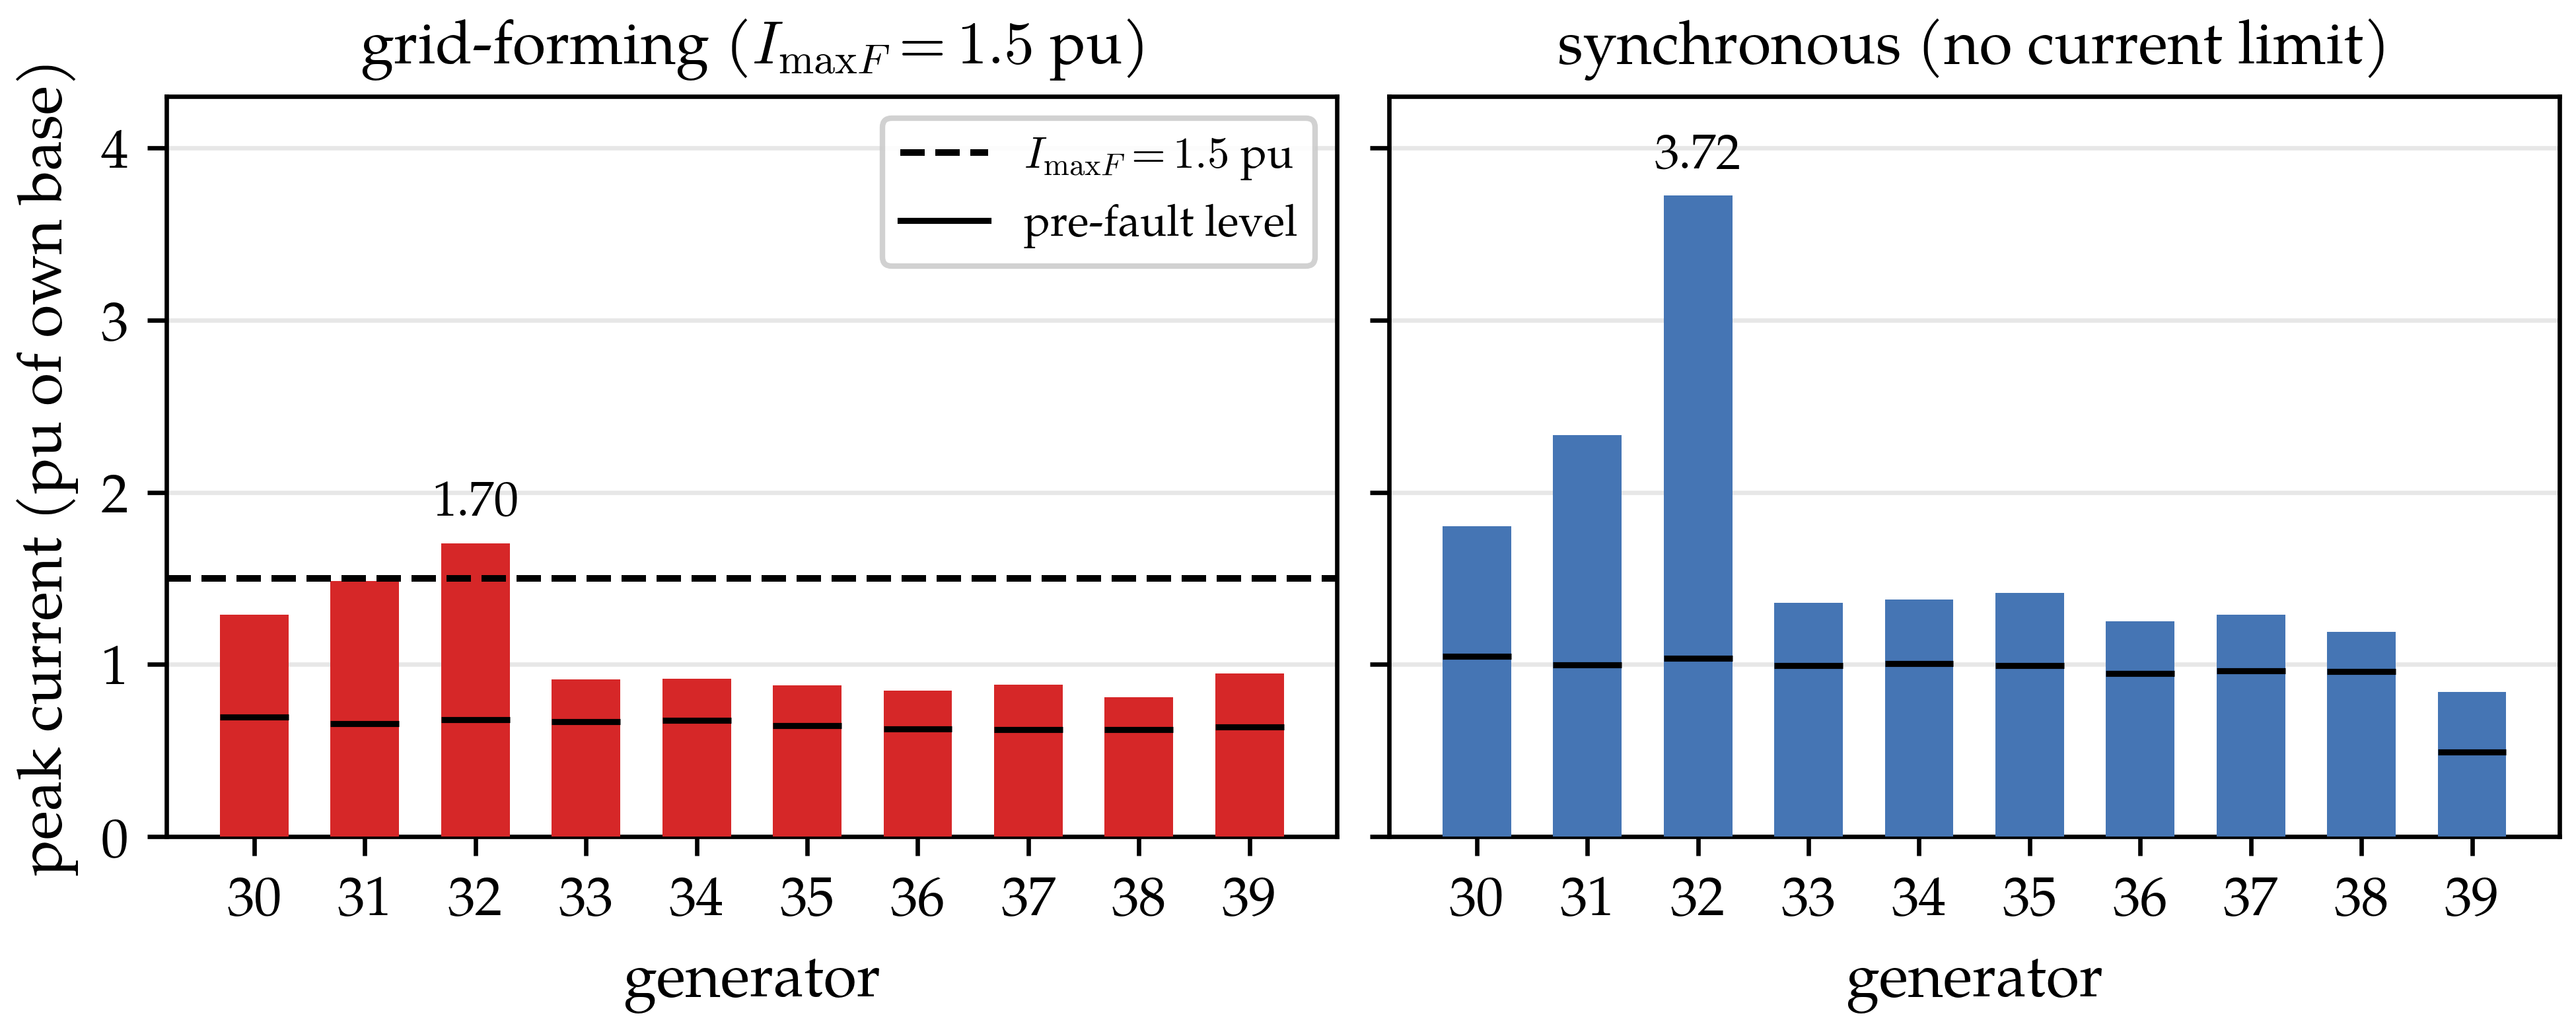
\includegraphics[width=\textwidth]{narr_peakI_pair}
\caption{Peak currents for the bus-10 disturbance on individual device bases, with the GFM transient-current setting at 1.5 per unit. For the GFM units the quantity is the inverter's own current magnitude at its terminals (10~kV side of the step-up transformer); for the machines it is the RMS current on the 230~kV side.}
\label{fig:peaki}
\end{figure}

\begin{figure}[tbp]\centering
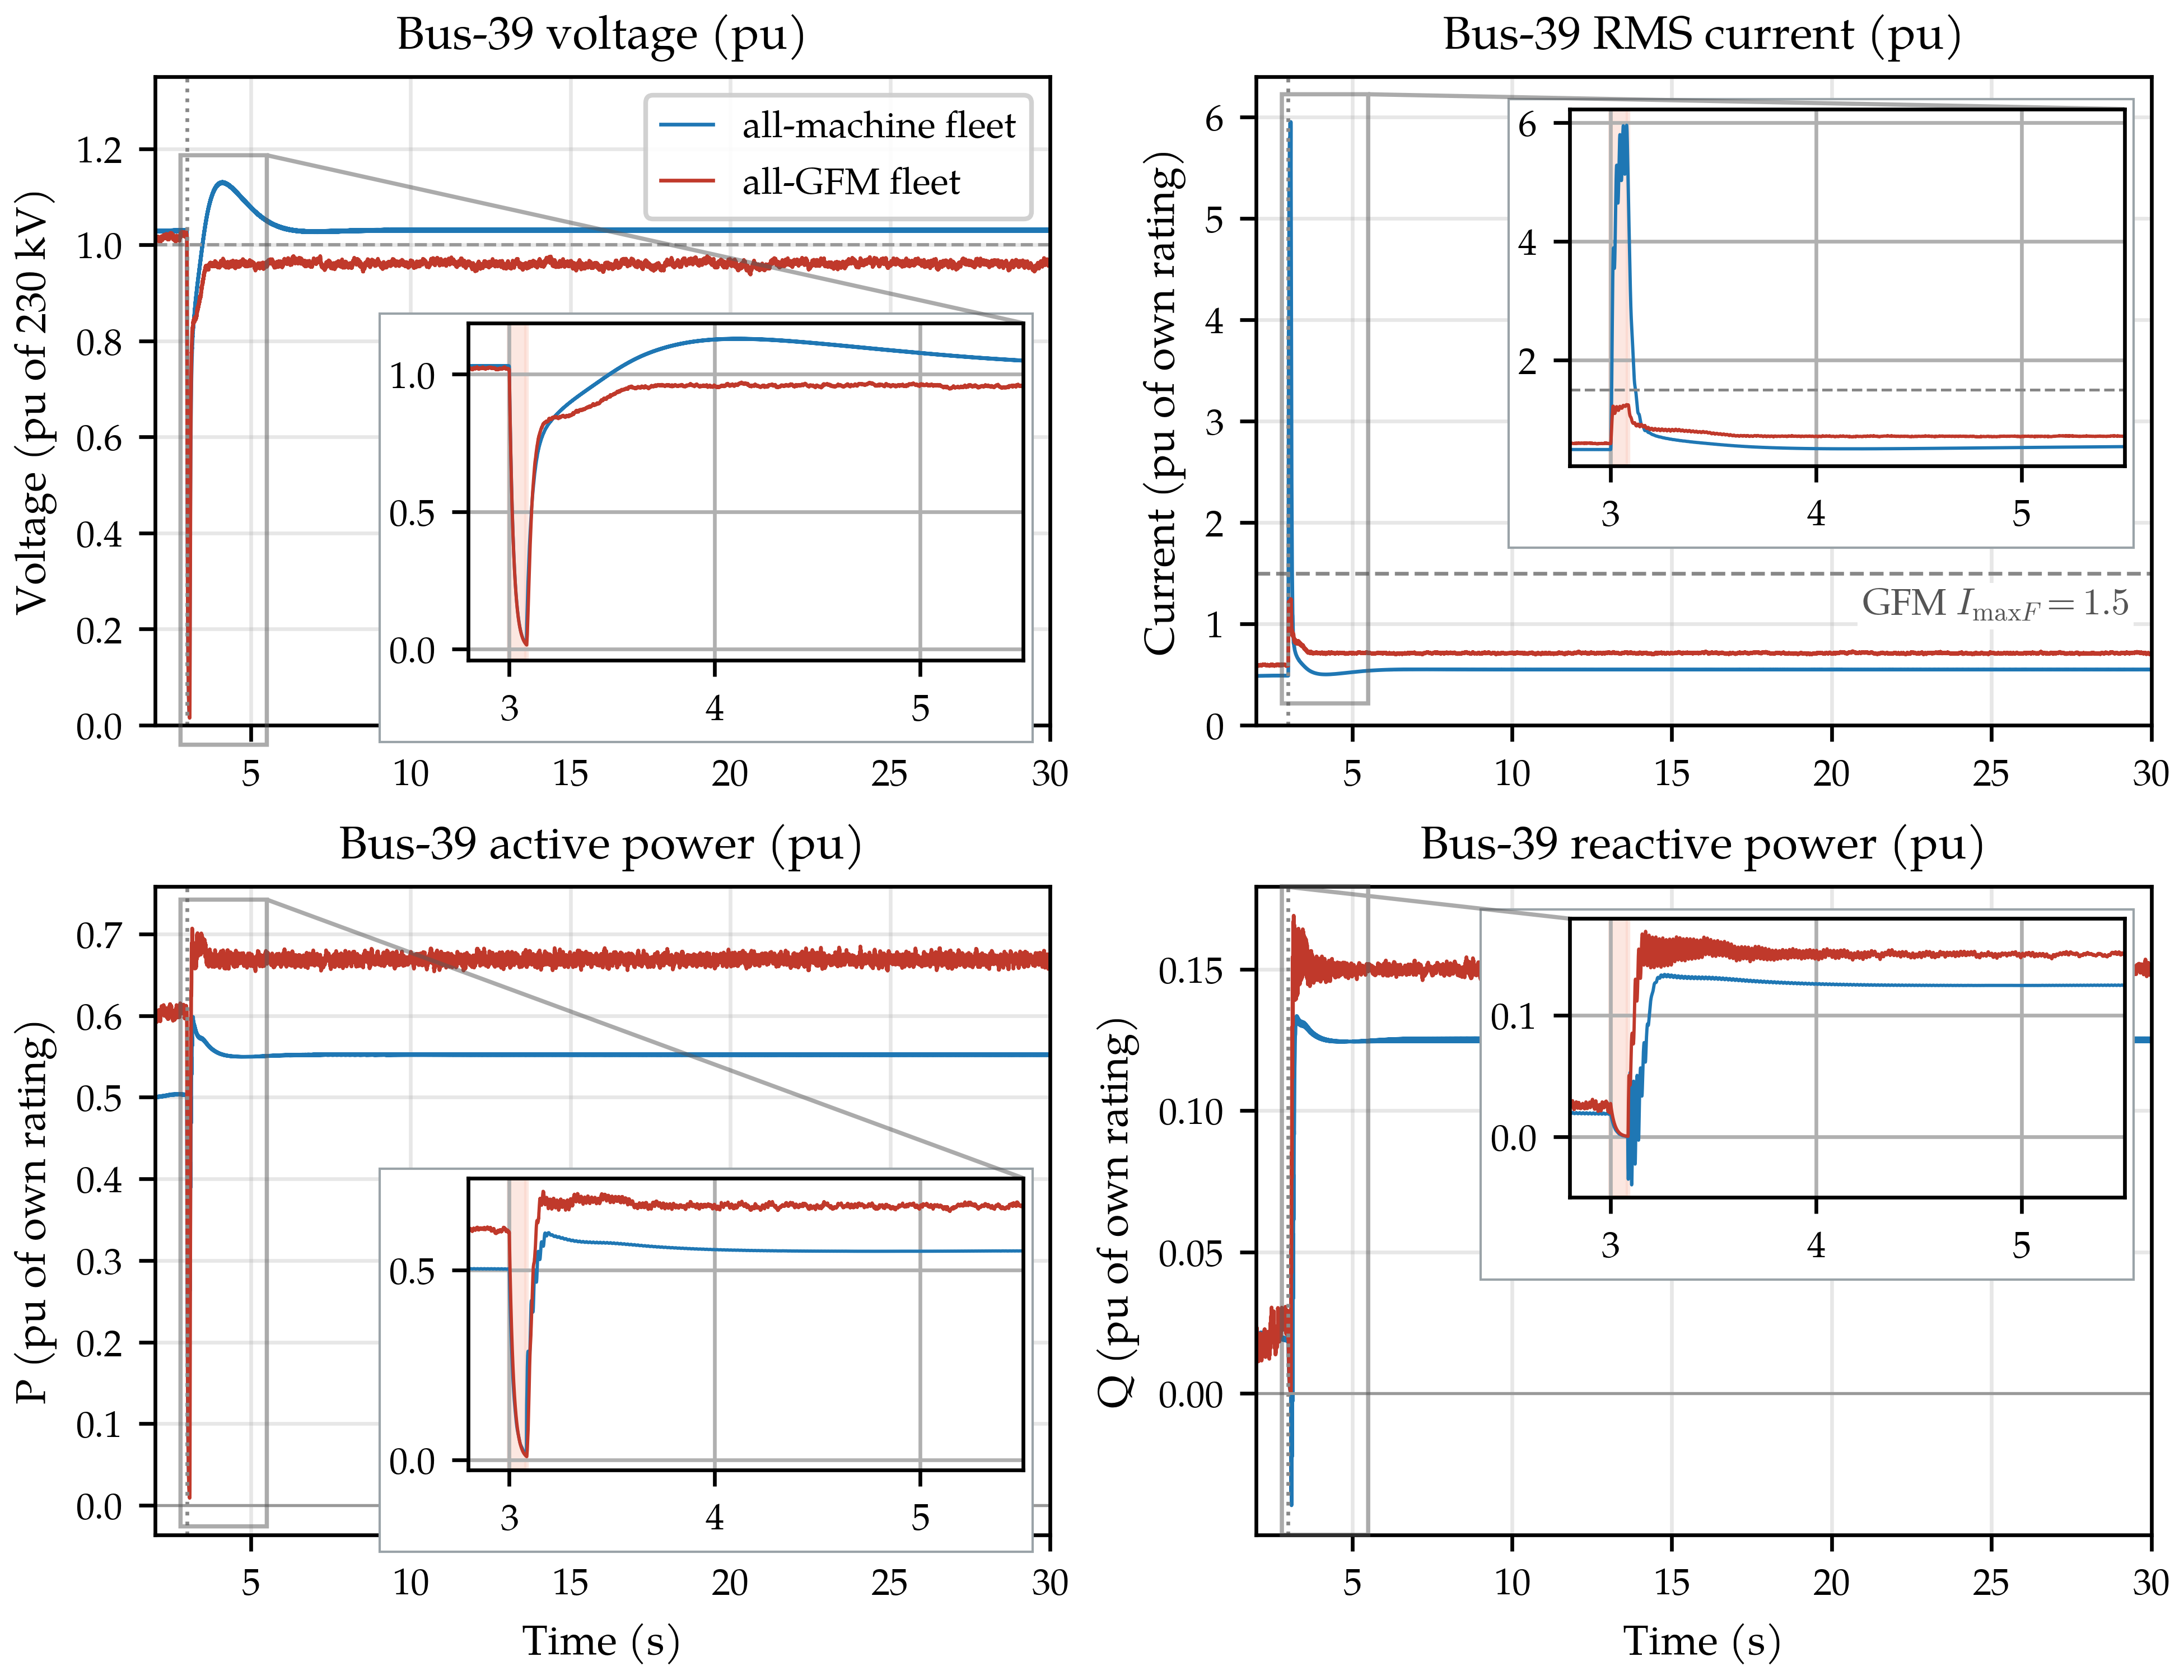
\includegraphics[width=\textwidth]{exec_gfm_vs_sync_bus39_pu}
\caption{Bus-39 responses to a five-cycle three-phase fault at bus~39, measured on the 230~kV side of the unit's step-up transformer: all-machine (blue) and all-GFM (red, $I_{\max F}=1.5$ per unit), each on its own device base (2000 and 1667~MVA). Clearing opens lines 1--39 and 9--39, which leaves the unit islanded with the bus-39 load.}
\label{fig:exec}
\end{figure}

\subsection{All-Synchronous Machine Fault Ride Through}
\label{sec:syncbaseline}
The all-machine system rides through the same reference fault as the all-GFM system. Its generator-bus active powers oscillate together at about 1~Hz, the inter-machine swing mode, and the oscillation persists for tens of seconds; the units nearest the fault, buses~31 and~32, settle faster. The stronger damping associated with the selected GFM controls helps interpret the contrast, as developed in Section~\ref{sec:dynamics}. Network conditions, voltage controls, and limiting also affect the complete transient response.

\subsection{Grid-Following Inverter Fault Ride Through}
\label{sec:gfl}
We also evaluated a PNNL-based GFL implementation in the testbed. It is the only inverter model in the 39-bus studies whose circuit includes explicit semiconductor switch elements: its average-value module carries a bridge of six IGBT and six diode elements, each a two-state switch with an on-state resistance and a snubber, whereas the REGFM\_A1 units are controlled voltage sources behind a reactance. The surrounding grid recovers within approximately one second, but the local voltage remains depressed over the plotted interval in Figures~\ref{fig:gflpocket} and~\ref{fig:gfldeadlock}. The filtered voltage remains below the dip threshold and the active and reactive current commands fall to zero. These signals point to a control-state response rather than demonstrating semiconductor breakdown.

We obtained post-fault operation in a modified implementation that replaced the current-source interface with a voltage-source representation. That modification changes the model under test and does not establish a general remedy for GFL control. We did not pursue the GFL study further in the first-year work. The original and modified outcomes therefore remain distinct from the main GFM replacement results.

\begin{figure}[tbp]\centering
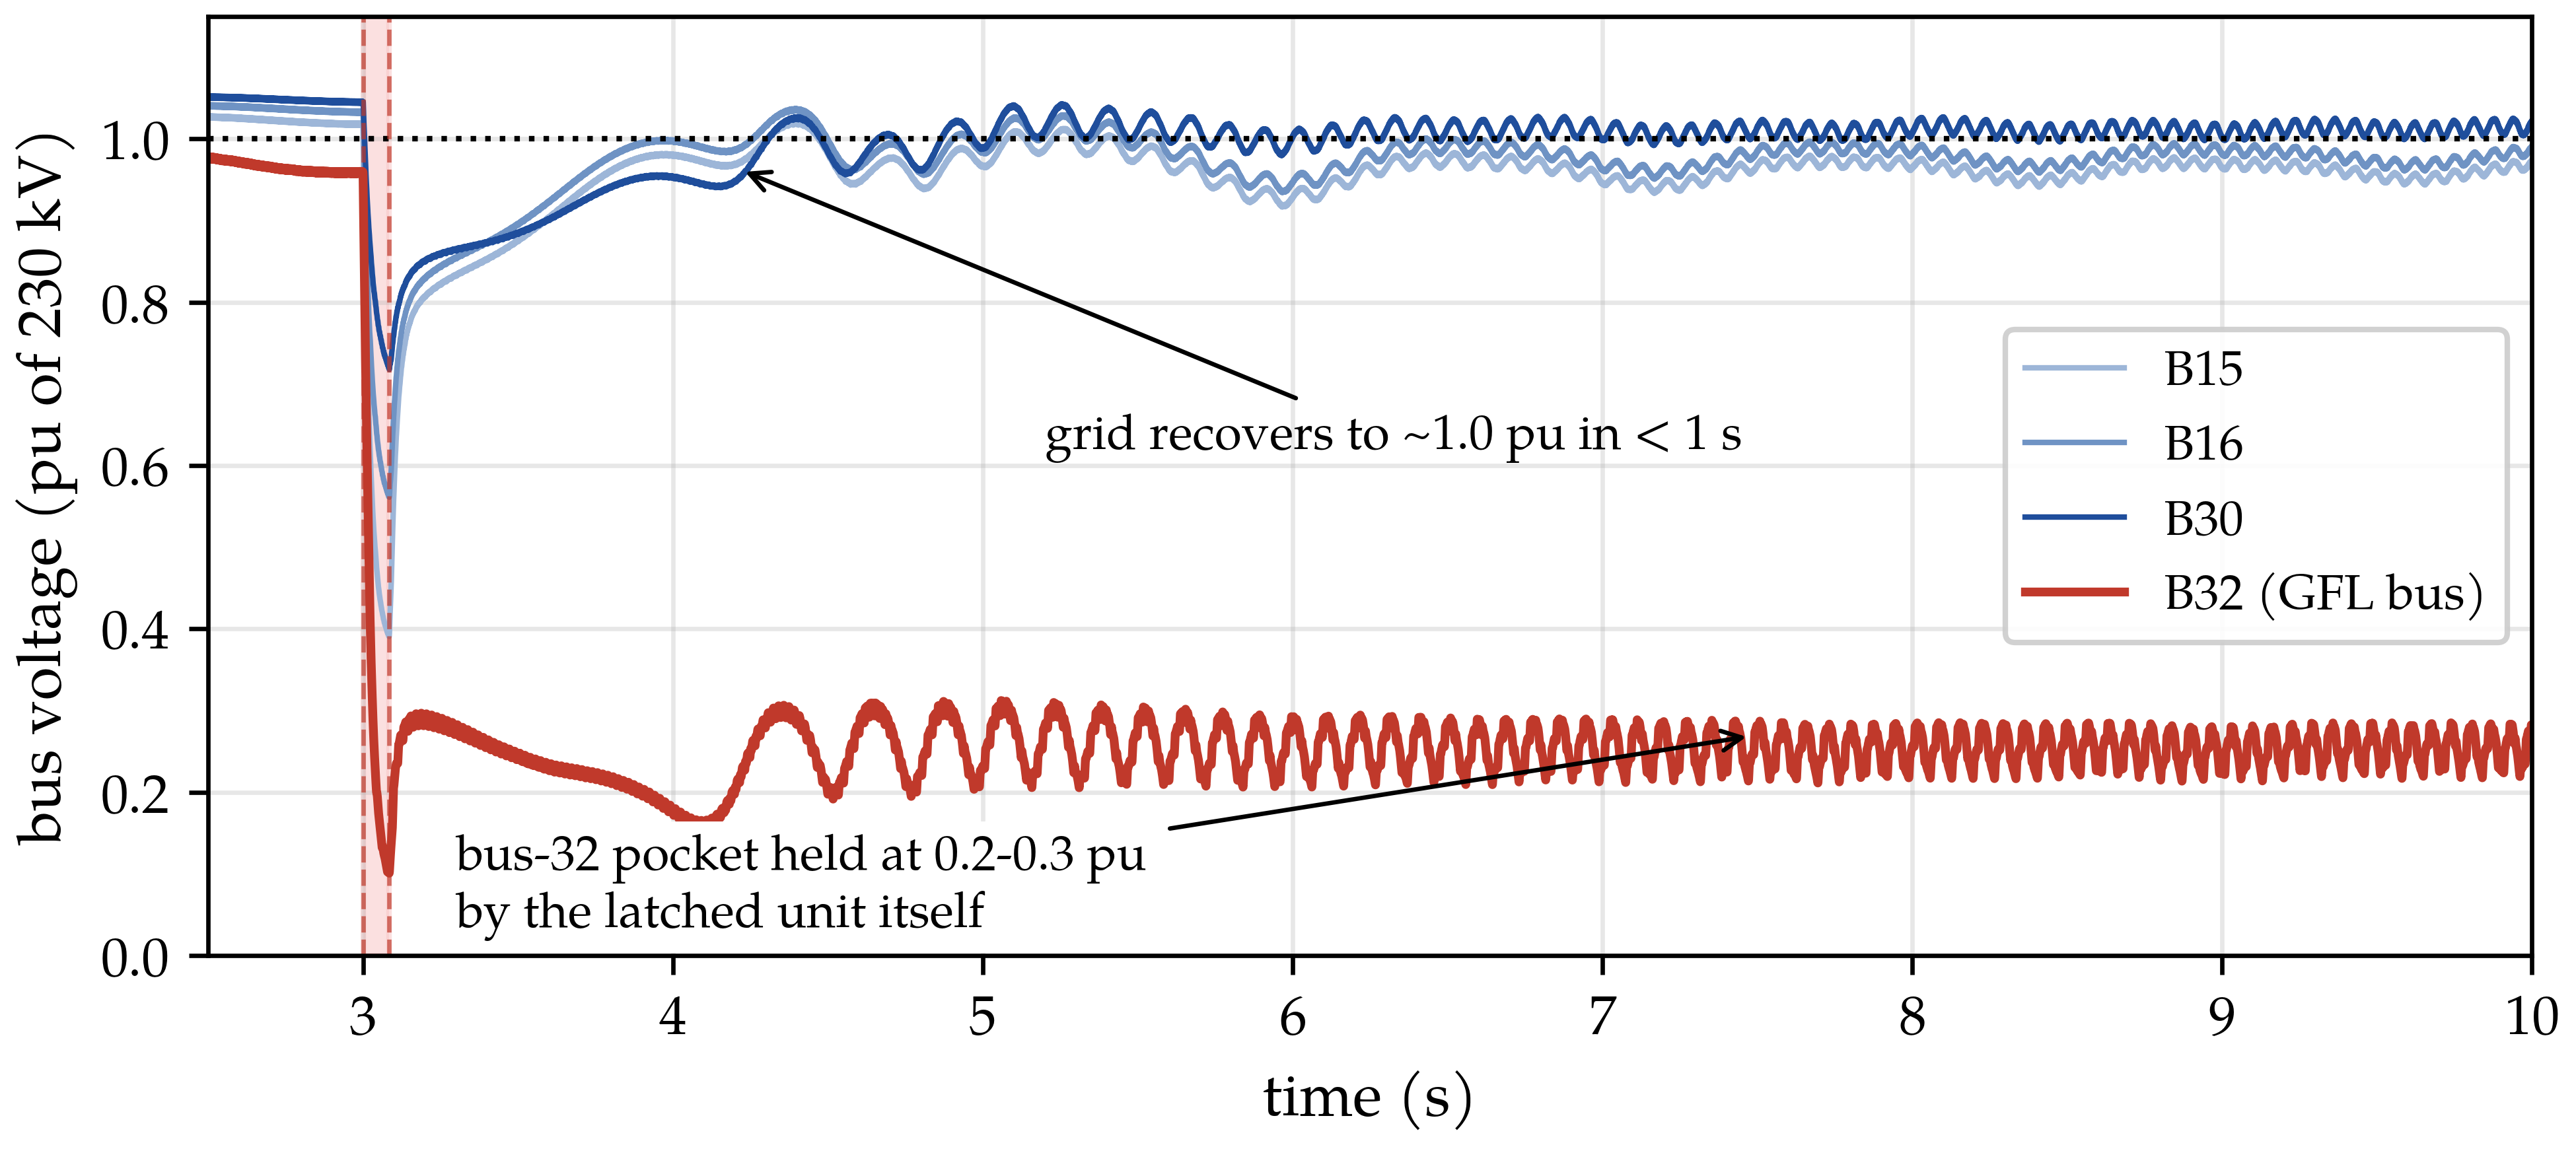
\includegraphics[width=\textwidth]{fig8a_gfl_pocket_vs_grid}
\caption{Original GFL implementation at bus~32: surrounding bus voltages recover while the local voltage remains depressed over the plotted interval.}
\label{fig:gflpocket}
\end{figure}

\begin{figure}[tbp]\centering
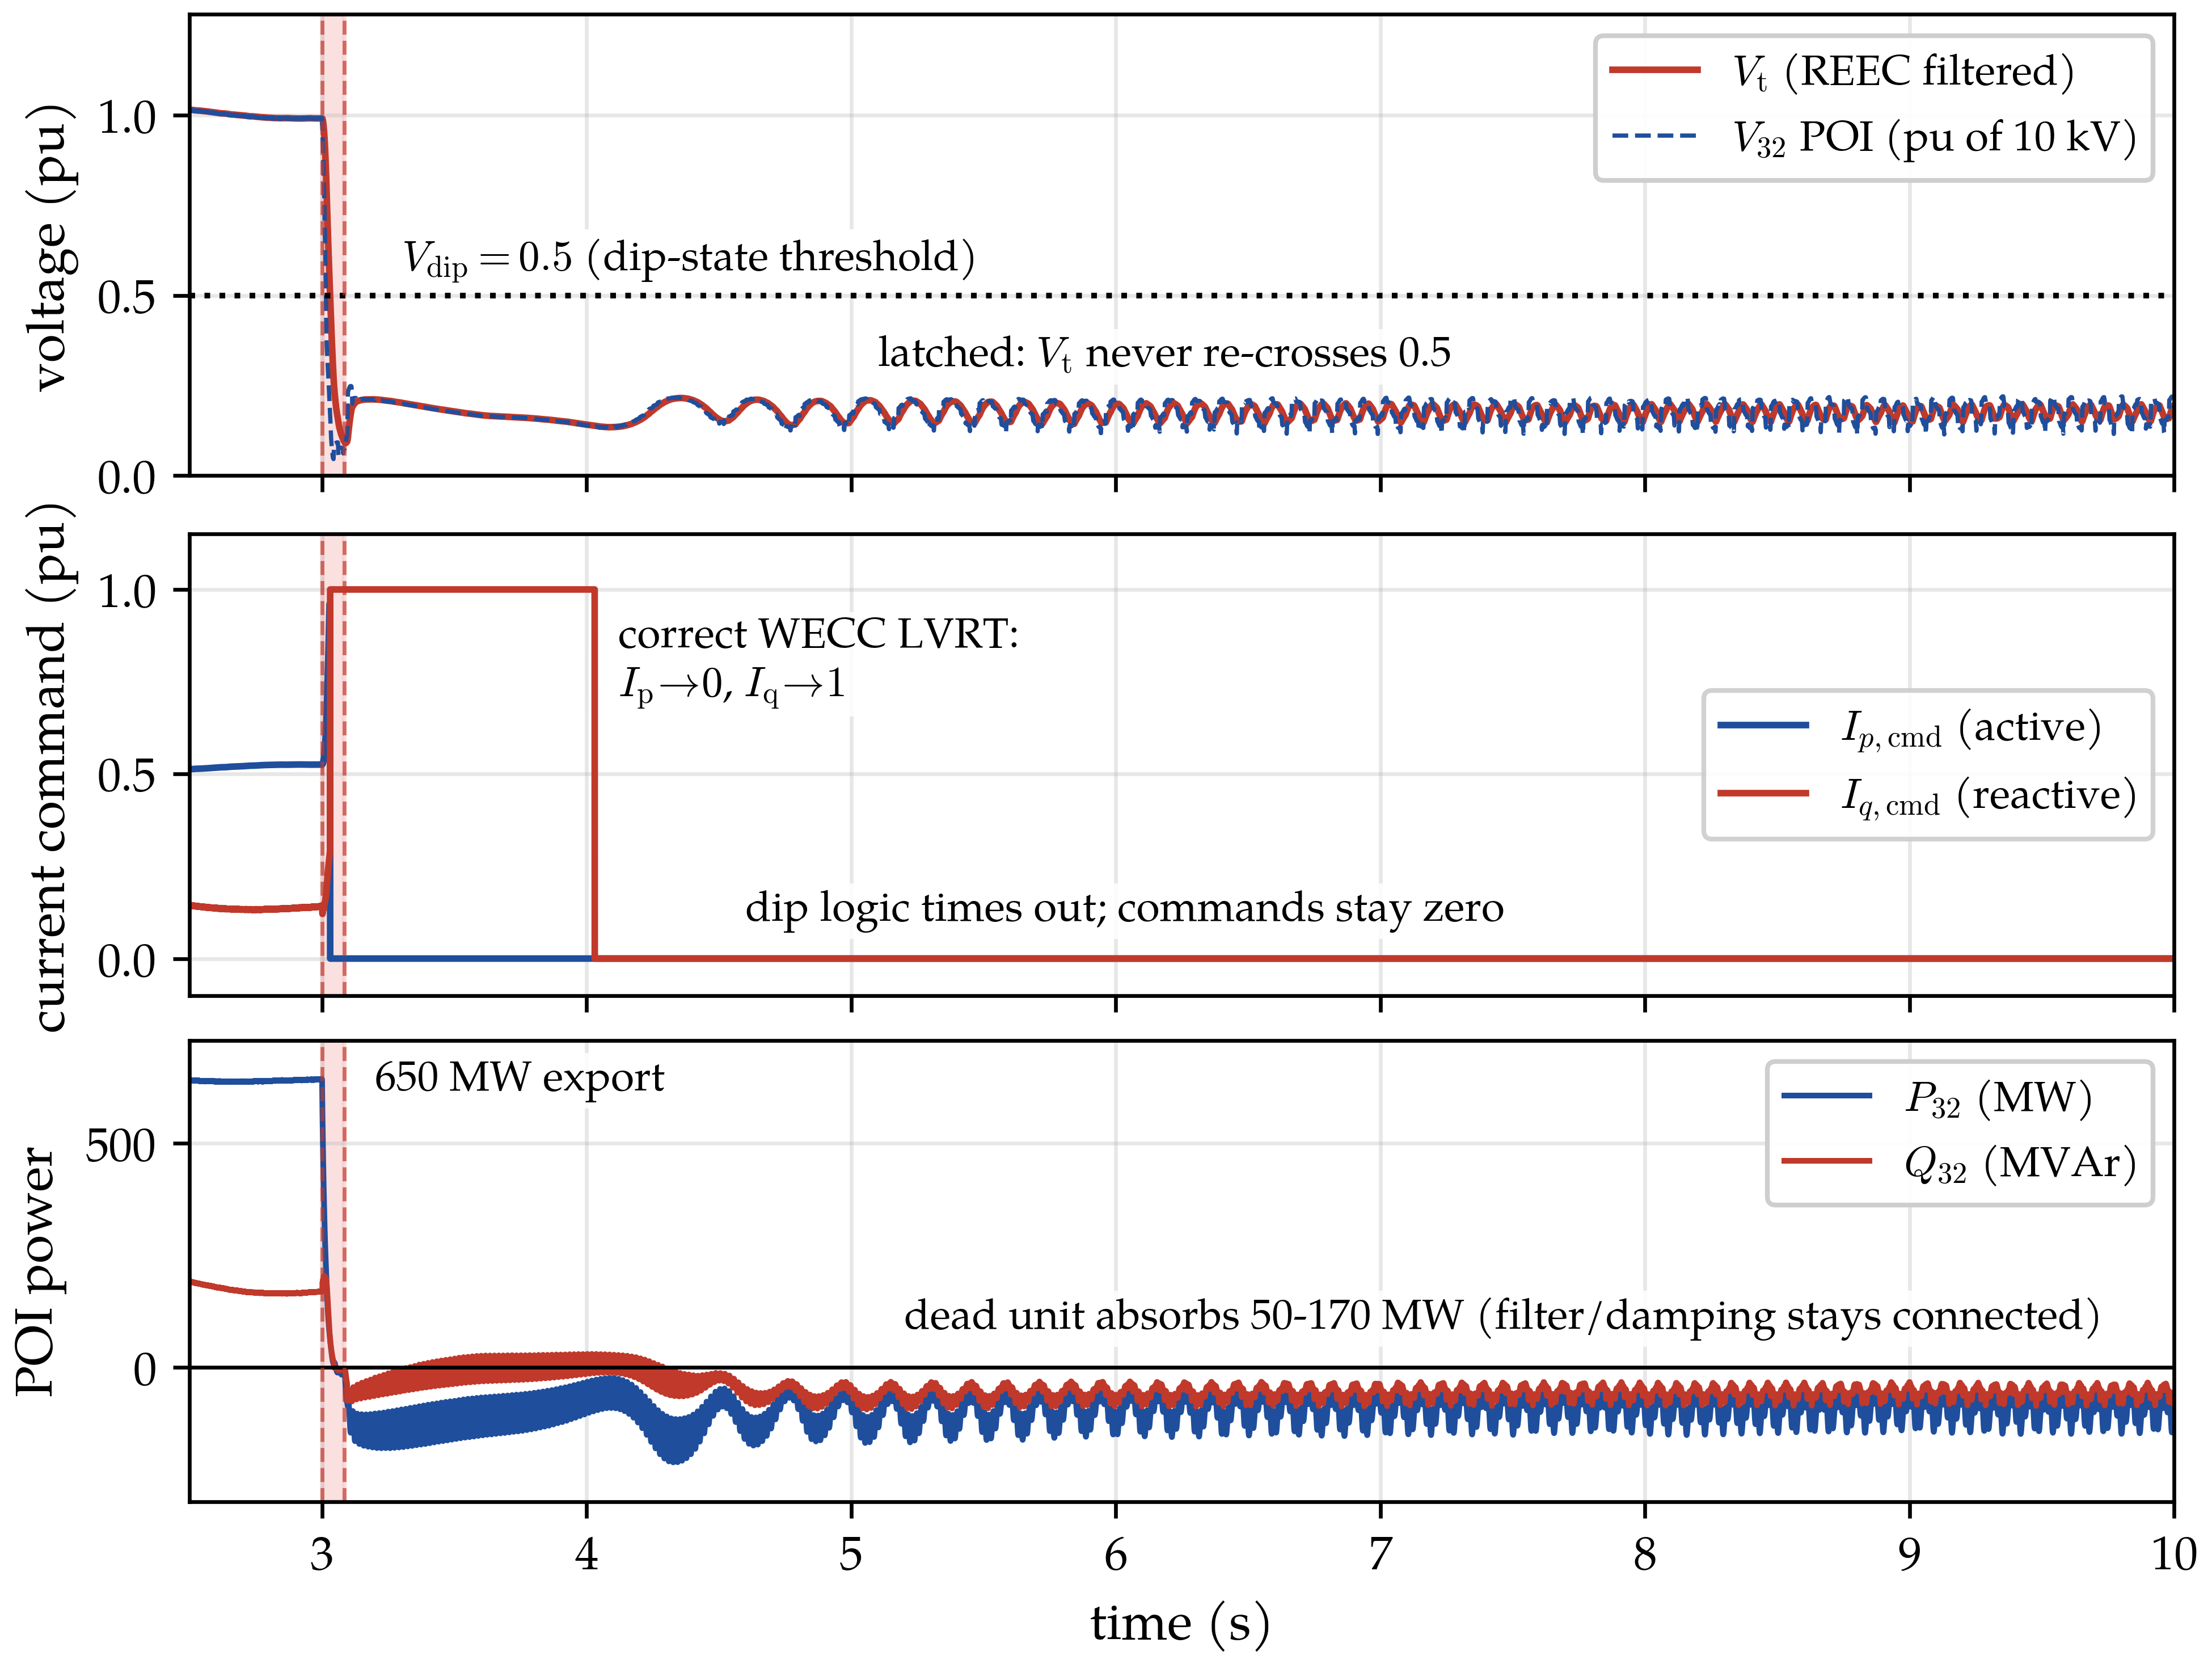
\includegraphics[width=\textwidth]{fig8b_gfl_deadlock}
\caption{Voltage-dip and current-command signals in the original GFL implementation: the filtered voltage stays below the dip threshold, and the active and reactive current commands go to zero. This grid-following model is the only inverter model in the 39-bus studies whose circuit includes explicit semiconductor switch elements (a six-IGBT, six-diode bridge inside its average-value module); the REGFM\_A1 units are controlled voltage sources behind a reactance.}
\label{fig:gfldeadlock}
\end{figure}

\subsection{Unbalanced Faults at Bus 14}
\label{sec:unbal}
Single-line-to-ground (phase A) and double-line-to-ground (phases A and B) faults were applied at bus~14 with the reference timing and clearing on the all-machine and all-GFM fleets, 10~s records (Table~\ref{tab:cases}). Figure~\ref{fig:unbal} shows the bus-16 RMS voltage through the fault and the peak RMS current of each unit on its own base. For the machines the peak unit currents are 1.51 and 2.22 per unit at bus~32 for the single-line and double-line faults, with instantaneous phase-current peaks of 2.14 and 4.12 per unit of rated peak, and the lowest monitored RMS voltage during the fault is 0.82 and 0.60 per unit at bus~15. For the GFM units the peak RMS currents are 0.85 and 1.08 per unit at bus~32, the internal current-magnitude signal stays below the 2.0 per-unit limit (peaks 0.95 and 1.40 per unit), and the lowest monitored RMS voltage is 0.81 and 0.57 per unit. In all four cases every unit rides through: post-fault active power returns to within 3.8\% (machines) and 0.6\% (GFM units) of its pre-fault value on every unit, and the frequency settles at 59.84--59.90~Hz for the machines and 60.00~Hz for the GFM fleet.

\begin{figure}[tbp]\centering
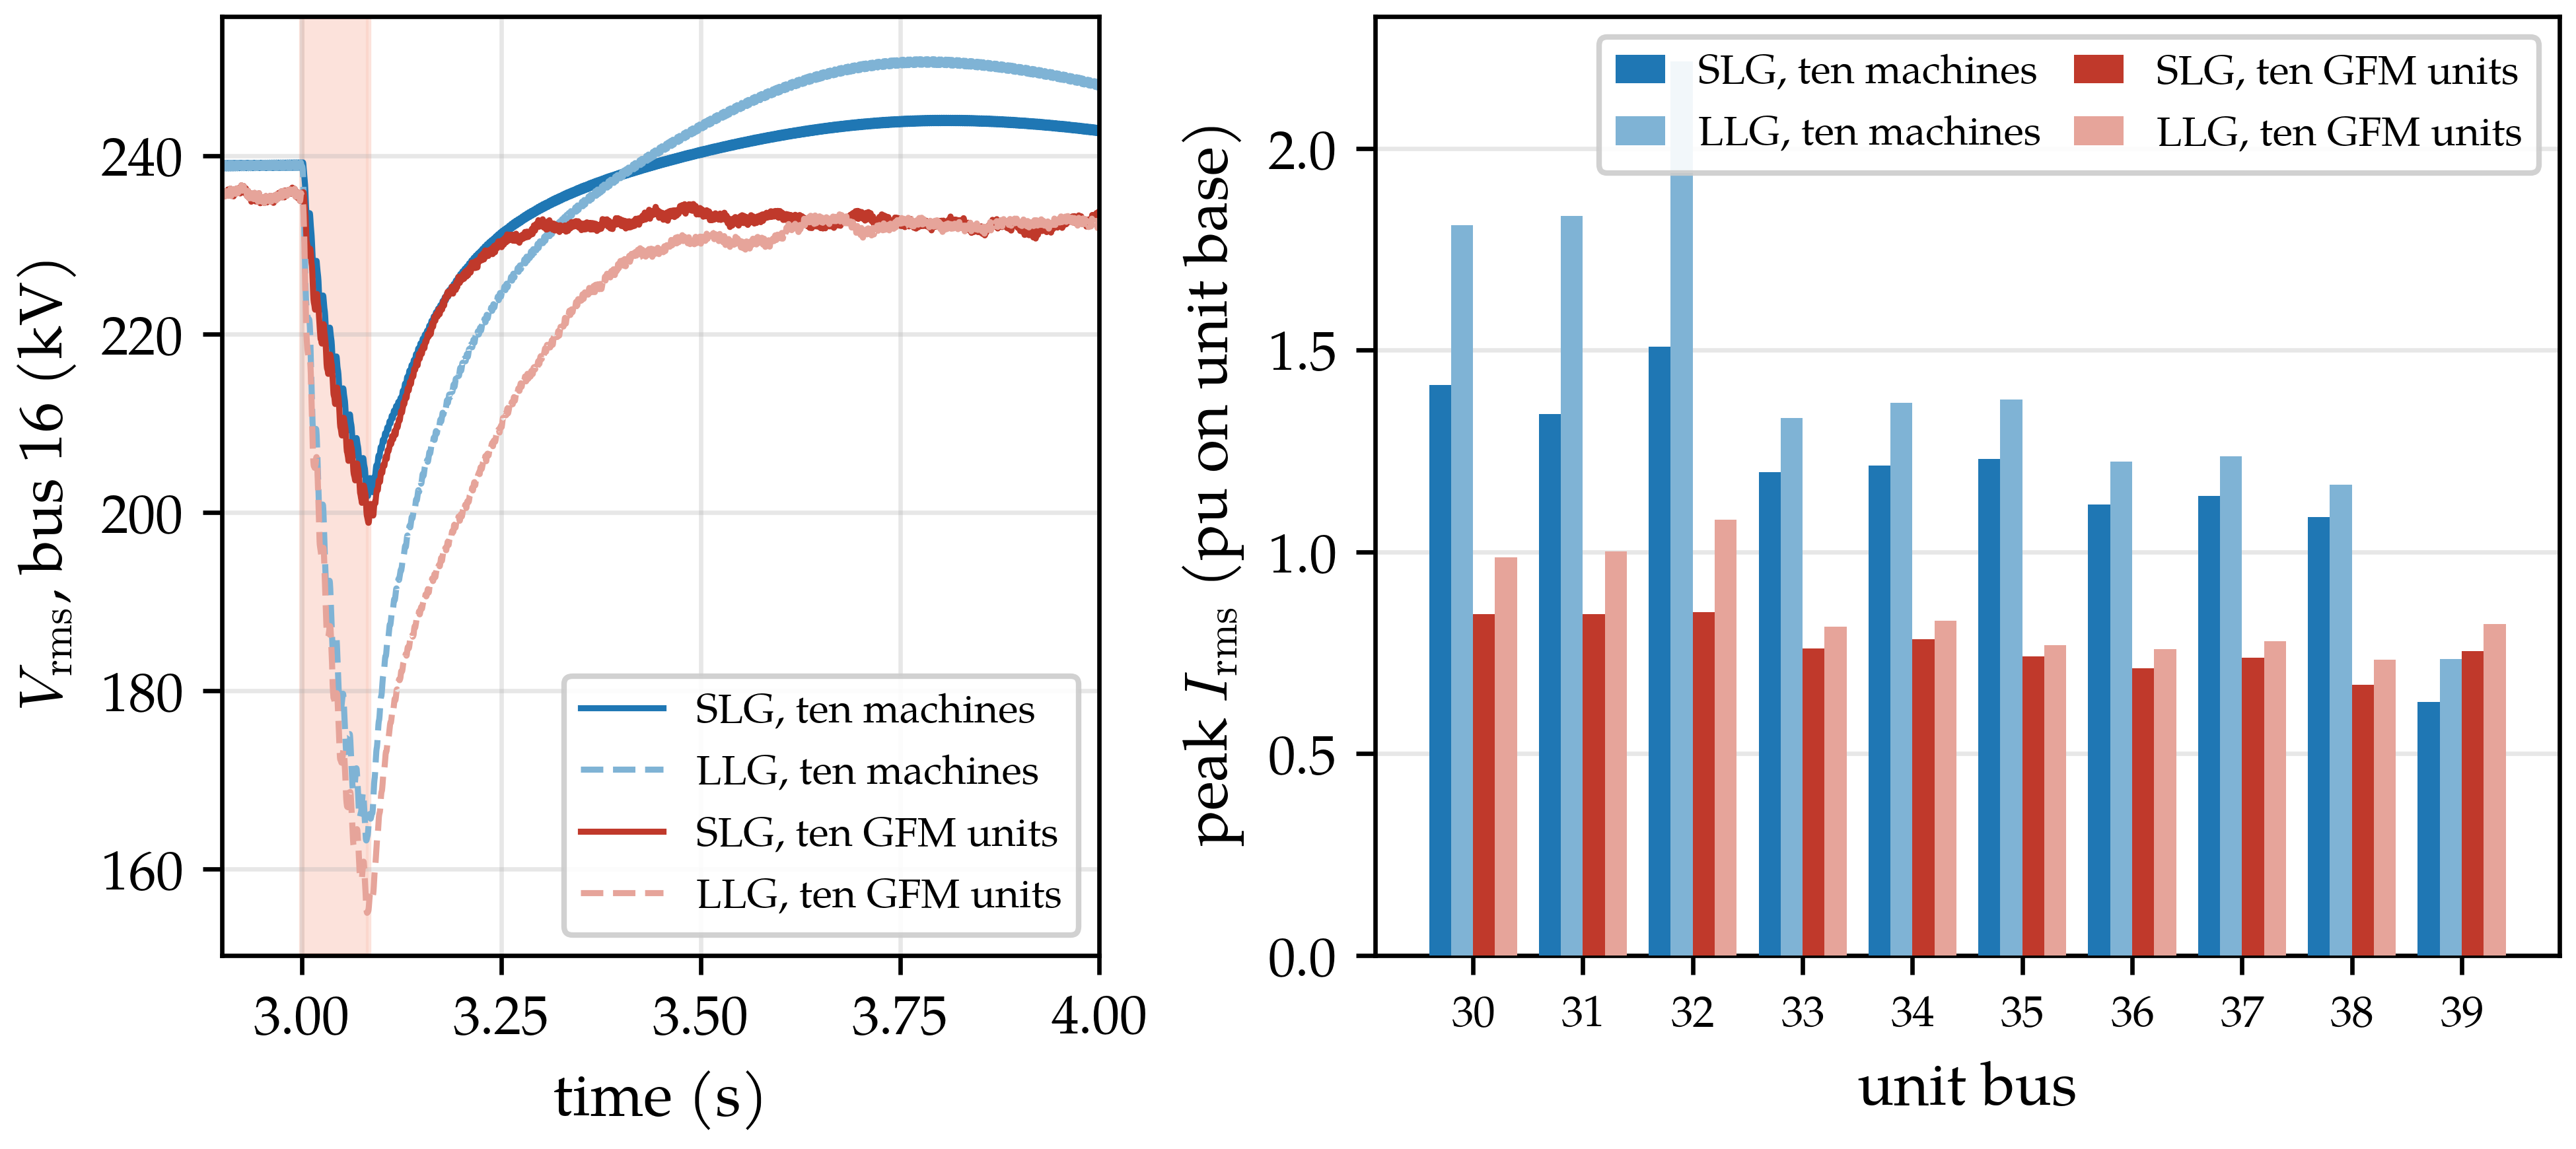
\includegraphics[width=\textwidth]{narr_unbal_bus14}
\caption{Unbalanced faults at bus~14, all-machine and all-GFM fleets, 10~s records with the reference timing and clearing. Left: bus-16 RMS voltage through the fault (SLG solid, LLG dashed); right: peak RMS current of each unit on its own base, on the 230~kV side of its step-up transformer.}
\label{fig:unbal}
\end{figure}

\section{Deriving Dynamic Models of a Droop-Based GFM Inverter and a Synchronous Machine}
\label{sec:dynamics}
The simulations in Section~\ref{sec:emt} show fault ride through and contrasting post-fault responses. To interpret those differences, we compare the dynamic equations of the machine and the droop-controlled inverter. Equivalent inertia opposes frequency acceleration, while equivalent damping opposes frequency deviation. These reduced descriptions connect device controls to the responses observed in the network.

A synchronous machine stores kinetic energy in its rotor, whereas an inverter generates its electrical phase through control. The two phase states can occupy analogous positions in reduced equations without representing the same physical mechanism. An inverter draws energy from its DC source and circuit storage; an equivalent inertia coefficient does not imply a rotating energy store. The analogy is useful within its assumptions, not a replacement for network, voltage-control, and limiter dynamics.

Prior work develops droop-converter stability analysis with current limitation \cite{huang2019}, examines the applicability of equal-area reasoning \cite{chatterjee2025eac}, and describes equivalent-circuit models \cite{chatterjee2025compel}. Interaction-energy methods extend the analysis to multiple GFM inverters \cite{chatterjee2025ecce}. We use the swing-form development in \cite{chatterjee2026note} to compare the selected models. The following derivation establishes consistent frequency normalization before discussing the effects of limiting.

\subsection{Synchronous Machine Dynamic Model}
\label{sec:smmodel}
The classical model relates electrical power imbalance to rotor acceleration \cite{sauer1998,kundur1994}. Let $\omega_0=2\pi f_{\mathrm{n}}$ denote nominal electrical angular frequency in rad/s, where $f_{\mathrm{n}}$ is nominal frequency in Hz. Define the normalized frequency deviation as $\Delta\bar{\omega}=(\omega_{\mathrm{e}}-\omega_0)/\omega_0$, in per unit (the bar marks a per-unit quantity). Let $\theta_{\mathrm{E}}$ be the phase of the internal voltage and $\theta_{\mathrm{V}}$ that of the grid voltage, both measured from the synchronous reference; the electrical phase displacement that sets the power transfer is the angle across the reactance, $\delta=\theta_{\mathrm{E}}-\theta_{\mathrm{V}}$. With the stiff grid as the reference, $\theta_{\mathrm{V}}$ is constant and $\dot\delta=\dot\theta_{\mathrm{E}}=\omega_0\Delta\bar{\omega}$. With powers normalized on the machine apparent-power base,
\begin{equation}
\frac{2H}{\omega_0}\,\ddot\delta+\frac{D}{\omega_0}\,\dot\delta=p_{\mathrm{m}}-p_{\mathrm{e}},
\label{eq:swingangle}
\end{equation}
where $H$ is the inertia constant in seconds and $D$ is normalized power per normalized frequency deviation. Mechanical input and electrical output are $p_{\mathrm{m}}$ and $p_{\mathrm{e}}$, respectively. The physical kinetic-energy definition is $H=J\omega_{\mathrm{m0}}^2/(2S_{\mathrm{base}})$, where $J$ is moment of inertia in kg\,m$^2$, $\omega_{\mathrm{m0}}$ is nominal mechanical speed in rad/s, and $S_{\mathrm{base}}$ is in VA. Electrical angular frequency equals mechanical angular speed multiplied by the number of pole pairs.

For constant voltage magnitudes connected through total reactance $X_{\mathrm{tot}}$, the electrical power is $p_{\mathrm{e}}=p_{\mathrm{max}}\sin\delta$. Here $p_{\mathrm{max}}=E'V/X_{\mathrm{tot}}$, with transient internal voltage $E'$, grid voltage $V$, and reactance expressed on compatible per-unit bases. Taking the stiff grid as the angle reference gives
\begin{equation}
M\ddot\delta=p_{\mathrm{m}}-p_{\mathrm{max}}\sin\delta-\frac{D}{\omega_0}\dot\delta,
\qquad M=\frac{2H}{\omega_0}.
\label{eq:swingeq}
\end{equation}
Figure~\ref{fig:smcircuit} shows this single-machine infinite-bus representation.

\begin{figure}[tbp]\centering
% Companion to tikz_gfm_basic_model: the classical synchronous-machine
% model in the same drawing convention (Sauer & Pai / Kundur): the
% transient EMF E'<delta behind the transient reactance X'_{\mathrm{d}}, feeding
% the grid at V<delta_V. E' and delta are set by the field circuit and
% the rotor's swing dynamics rather than by a controller.
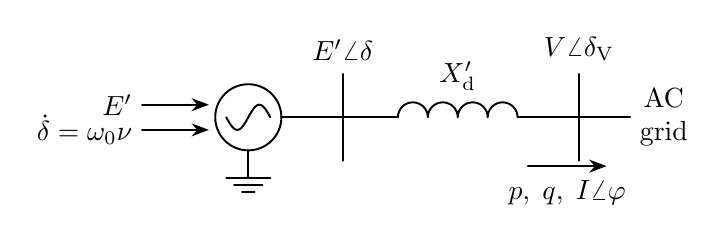
\begin{tikzpicture}[x=1cm, y=1cm, line cap=round, line join=round,
    wire/.style={line width=0.7pt},
    lbl/.style={font=\normalsize},
    >={Stealth[length=2.2mm]}]
  \coordinate (src) at (0,0);
  \draw[wire] (src) circle (0.42);
  \draw[wire] plot[domain=-0.28:0.28, samples=40, smooth]
      ({\x}, {0.16*sin(deg(\x*3.1416/0.28))});
  \draw[wire] (src) ++(0,-0.42) -- ++(0,-0.35) coordinate (gnd);
  \draw[wire] (gnd) ++(-0.28,0) -- ++(0.56,0);
  \draw[wire] (gnd) ++(-0.18,-0.09) -- ++(0.36,0);
  \draw[wire] (gnd) ++(-0.08,-0.18) -- ++(0.16,0);
  % what sets the source: field (E') and rotor swing (delta)
  \draw[->, wire] (-1.35,0.16) -- (-0.5,0.16);
  \draw[->, wire] (-1.35,-0.16) -- (-0.5,-0.16);
  \node[lbl, left] at (-1.35,0.16) {$E'$};
  \node[lbl, left] at (-1.35,-0.16) {$\dot\delta=\omega_0\nu$};
  \draw[wire] (src) ++(0.42,0) -- (1.2,0);
  \draw[wire] (1.2,-0.55) -- (1.2,0.55);
  \node[lbl, above] at (1.2,0.6) {$E'\angle\delta$};
  \draw[wire] (1.2,0) -- (1.9,0);
  \draw[wire] (1.9,0)
     arc[start angle=180, end angle=0, radius=0.19]
     arc[start angle=180, end angle=0, radius=0.19]
     arc[start angle=180, end angle=0, radius=0.19]
     arc[start angle=180, end angle=0, radius=0.19];
  \node[lbl, above] at (2.66,0.22) {$X'_{\mathrm{d}}$};
  \draw[wire] (3.42,0) -- (4.2,0);
  \draw[wire] (4.2,-0.55) -- (4.2,0.55);
  \node[lbl, above] at (4.2,0.6) {$V\angle\delta_{\mathrm{V}}$};
  \draw[wire] (4.2,0) -- (4.85,0);
  \node[lbl, right, align=center] at (4.85,0) {AC\\grid};
  \draw[->, wire] (3.55,-0.62) -- (4.55,-0.62);
  \node[lbl, below] at (4.05,-0.68) {$p,\;q,\;I\angle\varphi$};
\end{tikzpicture}

\caption{Classical synchronous-machine model: transient internal voltage $E^\prime\angle\theta_{\mathrm{E}}$, its magnitude set by the field circuit, behind reactance $X^\prime_{\mathrm{d}}$ and connected to the grid at $V\angle\theta_{\mathrm{V}}$. The displacement $\delta=\theta_{\mathrm{E}}-\theta_{\mathrm{V}}$ is tied to rotor motion and satisfies $\dot\delta=\omega_0\Delta\bar{\omega}$.}
\label{fig:smcircuit}
\end{figure}

\subsection{GFM Inverter Dynamic Model}
\label{sec:gfmmodel}
The simplified GFM model used in the analysis is a controllable voltage source behind coupling reactance $X_{\mathrm{L}}$ \cite{du2023a1}. Its topology resembles the classical machine circuit, but the controller determines its internal voltage magnitude and phase. Figure~\ref{fig:gfmcircuit} shows the interface and Figure~\ref{fig:gfmequiv} shows the corresponding Norton equivalent used in a network solution. The equivalent circuit does not change the resource's GFM control classification.

The controlled source has magnitude $E$ and phase $\theta_{\mathrm{E}}$, while the terminal grid voltage has magnitude $V$ and phase $\theta_{\mathrm{V}}$; as for the machine, the displacement $\delta=\theta_{\mathrm{E}}-\theta_{\mathrm{V}}$ across the coupling reactance sets the power transfer. In the machine representation, the field circuit sets the internal voltage magnitude and rotor motion determines its phase. In the GFM representation, the power and voltage controls perform the analogous functions. The controller acts on filtered power measurements rather than directly applying its droop gain to instantaneous unfiltered power.

In the analyzed runs the REGFM\_A1 controls are the $P$--$f$ droop of Equation~\eqref{eq:drooplaw}, whose frequency is integrated to the internal phase $\theta_{\mathrm{E}}$; the $Q$--$V$ droop with the voltage regulator ($k_{\mathrm{pv}}=0$, $k_{\mathrm{iv}}=5.86$~pu/s, $E_{\max}=1.15$, VFlag~$=1$, regulating the point-of-interconnection voltage); the reactive limits $Q_{\max}=-Q_{\min}=0.44$; the overload controller ($k_{\mathrm{ppmax}}=0.01$, $k_{\mathrm{ipmax}}=0.1$~pu/s), which acts only while filtered power exceeds $P_{\max}$ ($P_{\max}=0.9$, $P_{\min}=0$ in the single-device and inertia-test cases; $P_{\max}=2.0$, $P_{\min}=-0.9$ in the 39-bus cases, where it never engages); and the transient current limit $I_{\max F}$. The plant-controller references $P_{\mathrm{ref}}$, $Q_{\mathrm{ref}}$, and $V_{\mathrm{ref}}$ are held at their initialized values. The model exposes no inertia constant (Figure~\ref{fig:pscada1params}); its equivalent inertia is the filtered-droop quantity $T_{\mathrm{Pf}}/2m_{\mathrm{p}}$ of Equation~\eqref{eq:heqdeq} only. No secondary control, that is, no slower loop that returns frequency and voltage to their reference values after the droop response (plant-level integral control or automatic generation control), acts in any run \cite{du2023a1}. The post-fault operating points are the droop equilibria, and the effect of such a loop on stability is not assessed here. Figures~\ref{fig:controlblocks} and~\ref{fig:gfmblocks} show the machine governor path and the inverter controls as configured.

Figure~\ref{fig:controlblocks} reads as follows. The speed error $P_{\mathrm{ref}}-\omega-R\,\tilde P_{\mathrm{e}}$, with Rselect~$=1$ selecting the electrical power $P_{\mathrm{e}}$ filtered by $T_{\mathrm{pelec}}$, is clipped to [minerr, maxerr] $=\pm0.055$ per unit, so a speed error larger than 0.055 per unit (3.3~Hz) produces no further governor action. The clipped error drives the proportional gain and the integral branch; the integrator input $(K_{\mathrm{igov}}/K_{\mathrm{pgov}})(\mathit{fsr}-s_2)$ equals $K_{\mathrm{igov}}$ times the error while the governor is selected and tracks \textit{fsr} otherwise, which is the PES-TR1 anti-windup implementation of the PI controller. The load limiter ($L_{\mathrm{dref}}$, $K_{\mathrm{pload}}$, $K_{\mathrm{iload}}$, with the exhaust-temperature path through $T_{\mathrm{sa}}$, $T_{\mathrm{sb}}$, and $T_{\mathrm{fload}}$) and the acceleration limiter ($A_{\mathrm{set}}$, $K_{\mathrm{a}}$, $T_{\mathrm{a}}$) use the same tracking structure. The Low Value Select block compares the three fuel demands, governor (\textit{fsrn}), load limiter (\textit{fsrt}), and acceleration limiter (\textit{fsra}), and passes the smallest to the valve as \textit{fsr}, so whichever controller asks for the least fuel is in control. The valve stroke is rate-limited ($R_{\mathrm{open}}$, $R_{\mathrm{close}}$) and position-limited ($v_{\min}$, $v_{\max}$); with Flag~$=1$ the fuel flow \textit{Wf} is the stroke times speed, and $P_{\mathrm{mech}}=K_{\mathrm{turb}}(\mathit{Wf}-W_{\mathrm{fnl}})$ through the $T_{\mathrm{c}}$, $T_{\mathrm{b}}$ lead-lag. The only integral term in the governor path is $K_{\mathrm{igov}}$.

Figure~\ref{fig:gfmblocks} redraws the outer controls from Figures~3(a), 3(b), and~4 of the specification \cite{du2023a1}; its inputs $P_{\mathrm{inv}}$, $Q_{\mathrm{inv}}$, and $V_{\mathrm{inv}}$ have already passed through the $T_{\mathrm{Pf}}$, $T_{\mathrm{Qf}}$, and $T_{\mathrm{Vf}}$ measurement filters. In the $P$--$f$ droop, $\Delta\omega=\omega_0\,[m_{\mathrm{p}}(P_{\mathrm{ref}}-P_{\mathrm{inv}})+\Delta\omega_{\mathrm{OL}}]$, which is $\omega_0\Delta\bar{\omega}$ of Equation~\eqref{eq:drooplaw} with the overload term added, is integrated to $\delta_{\mathrm{droop}}$; the overload mitigation term $\Delta\omega_{\mathrm{OL}}$ is nonzero only above $P_{\max}$ or below $P_{\min}$ because its two branches are limited to non-positive and non-negative values. In the $Q$--$V$ droop, VFlag~$=1$ selects the proportional-integral voltage regulator that drives the point-of-interconnection voltage $V_{\mathrm{inv}}$ to $V_{\mathrm{cmd}}$, with its output limited to $[E_{\min},E_{\max}]=[0,1.15]$; the $Q_{\max}/Q_{\min}$ branches add to $V_{\mathrm{cmd}}$ only beyond the $\pm0.44$ per-unit limits. In the fault current limiter, while $I<I_{\max F}$ the internal voltage is the droop output; once $I\ge I_{\max F}$ it is recomputed from the terminal voltage and the coupling reactance so that the current magnitude is held at $I_{\max F}$ with its phase $\varphi$ unchanged. The integral terms are $k_{\mathrm{iv}}$, $k_{\mathrm{ipmax}}$, and $k_{\mathrm{iqmax}}$.


Active-power droop sets frequency, while reactive-power droop adjusts voltage magnitude. For the unsaturated reduced model, the normalized laws are
\begin{equation}
\Delta\bar{\omega}=m_{\mathrm{p}}\,\frac{1}{1+sT_{\mathrm{Pf}}}\,(p^{*}-p),\qquad
E=E_0+m_{\mathrm{q}}\,\frac{1}{1+sT_{\mathrm{Qf}}}\,(q^{*}-q),
\label{eq:drooplaw}
\end{equation}
where $p^{*},q^{*}$ are the power references, $p,q$ the normalized active and reactive power at the terminals, $s$ the Laplace variable, and $1/(1+sT_{\mathrm{Pf}})$ and $1/(1+sT_{\mathrm{Qf}})$ the first-order measurement filters. The frequency deviation is the rate of change of the controller-generated phase,
\begin{equation}
\Delta\bar{\omega}\triangleq\frac{\omega_{\mathrm{e}}-\omega_0}{\omega_0}=\frac{1}{\omega_0}\frac{\mathrm{d}\theta_{\mathrm{E}}}{\mathrm{d}t},
\label{eq:phasedef}
\end{equation}
with $\theta_{\mathrm{E}}$ measured from the synchronous reference, so against the stiff grid $\dot\delta=\omega_0\Delta\bar{\omega}$ as for the machine. Table~\ref{tab:droopvars} defines the droop variables and their units.

\begin{figure}[tbp]\centering
% Basic model of a grid-forming inverter, redrawn from Fig. 1 of the
% PNNL REGFM_A1 model specification (Du et al., PNNL-35110, 2023):
% a controllable voltage source E<delta_E behind the coupling
% reactance X_{\mathrm{L}}, feeding the AC grid at V<delta_V. Plain TikZ (no
% circuitikz) so it typesets in the document font.
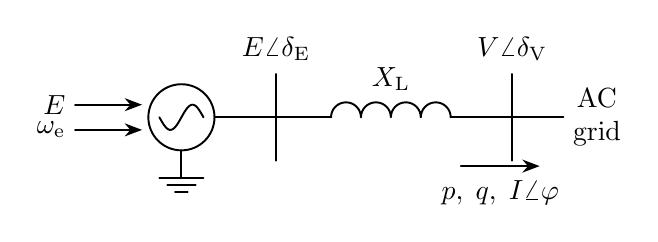
\begin{tikzpicture}[x=1cm, y=1cm, line cap=round, line join=round,
    wire/.style={line width=0.7pt},
    lbl/.style={font=\normalsize},
    >={Stealth[length=2.2mm]}]
  % --- controllable voltage source (circle with sine) -----------------
  \coordinate (src) at (0,0);
  \draw[wire] (src) circle (0.42);
  \draw[wire] plot[domain=-0.28:0.28, samples=40, smooth]
      ({\x}, {0.16*sin(deg(\x*3.1416/0.28))});
  \draw[wire] (src) ++(0,-0.42) -- ++(0,-0.35) coordinate (gnd);
  \draw[wire] (gnd) ++(-0.28,0) -- ++(0.56,0);
  \draw[wire] (gnd) ++(-0.18,-0.09) -- ++(0.36,0);
  \draw[wire] (gnd) ++(-0.08,-0.18) -- ++(0.16,0);
  % droop-controlled inputs E, omega
  \draw[->, wire] (-1.35,0.16) -- (-0.5,0.16);
  \draw[->, wire] (-1.35,-0.16) -- (-0.5,-0.16);
  \node[lbl, left] at (-1.35,0.16) {$E$};
  \node[lbl, left] at (-1.35,-0.16) {$\omega_{\mathrm{e}}$};
  % --- internal bus and coupling reactance ---------------------------
  \draw[wire] (src) ++(0.42,0) -- (1.2,0);
  \draw[wire] (1.2,-0.55) -- (1.2,0.55);              % internal bus bar
  \node[lbl, above] at (1.2,0.6) {$E\angle\delta_{\mathrm{E}}$};
  \draw[wire] (1.2,0) -- (1.9,0);
  % inductor coil: four bumps
  \draw[wire] (1.9,0)
     arc[start angle=180, end angle=0, radius=0.19]
     arc[start angle=180, end angle=0, radius=0.19]
     arc[start angle=180, end angle=0, radius=0.19]
     arc[start angle=180, end angle=0, radius=0.19];
  \node[lbl, above] at (2.66,0.22) {$X_{\mathrm{L}}$};
  \draw[wire] (3.42,0) -- (4.2,0);
  % --- terminal bus and grid ----------------------------------------
  \draw[wire] (4.2,-0.55) -- (4.2,0.55);
  \node[lbl, above] at (4.2,0.6) {$V\angle\delta_{\mathrm{V}}$};
  \draw[wire] (4.2,0) -- (4.85,0);
  \node[lbl, right, align=center] at (4.85,0) {AC\\grid};
  % power / current flow arrow toward the grid
  \draw[->, wire] (3.55,-0.62) -- (4.55,-0.62);
  \node[lbl, below] at (4.05,-0.68) {$p,\;q,\;I\angle\varphi$};
\end{tikzpicture}

\caption{Simplified inverter model used in the analysis, after Figure~1 of the REGFM\_A1 specification \cite{du2023a1}: a controllable voltage source $E\angle\theta_{\mathrm{E}}$ behind coupling reactance $X_{\mathrm{L}}$ delivers active and reactive power to the grid at $V\angle\theta_{\mathrm{V}}$. Under unsaturated filtered droop, $\dot\theta_{\mathrm{E}}=\omega_0\Delta\bar{\omega}$.}
\label{fig:gfmcircuit}
\end{figure}

\begin{figure}[tbp]\centering
% Inverter equivalent circuits, redrawn from Fig. 2 of the PNNL
% REGFM_A1 model specification (Du et al., PNNL-35110, 2023):
% (a) internal voltage source E<delta_E behind coupling reactance X_{\mathrm{L}};
% (b) its Norton equivalent, current source I_{\mathrm{N}}<phi_N in parallel with
% admittance Y_{\mathrm{L}}, which is what the network solver sees.
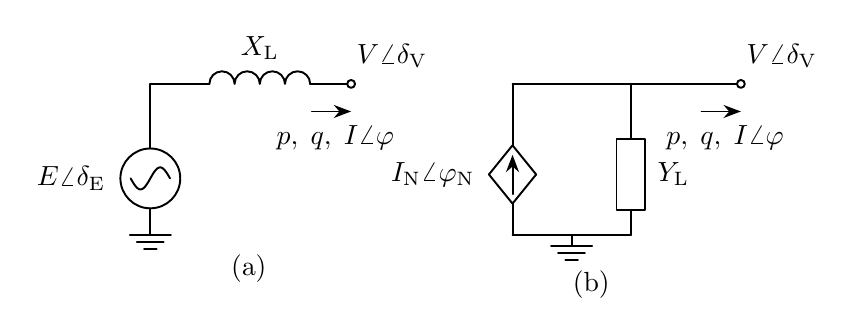
\begin{tikzpicture}[x=1cm, y=1cm, line cap=round, line join=round,
    wire/.style={line width=0.7pt},
    lbl/.style={font=\normalsize},
    >={Stealth[length=2.2mm]}]
  % ================= (a) Thevenin form =================
  \begin{scope}[shift={(0,0)}]
    % source
    \draw[wire] (0,0) circle (0.38);
    \draw[wire] plot[domain=-0.25:0.25, samples=40, smooth]
        ({\x}, {0.14*sin(deg(\x*3.1416/0.25))});
    \node[lbl, left] at (-0.45,0) {$E\angle\delta_{\mathrm{E}}$};
    % ground below source
    \draw[wire] (0,-0.38) -- (0,-0.72);
    \draw[wire] (-0.26,-0.72) -- (0.26,-0.72);
    \draw[wire] (-0.17,-0.81) -- (0.17,-0.81);
    \draw[wire] (-0.08,-0.90) -- (0.08,-0.90);
    % up and across through the reactance
    \draw[wire] (0,0.38) -- (0,1.2) -- (0.75,1.2);
    \draw[wire] (0.75,1.2)
       arc[start angle=180, end angle=0, radius=0.16]
       arc[start angle=180, end angle=0, radius=0.16]
       arc[start angle=180, end angle=0, radius=0.16]
       arc[start angle=180, end angle=0, radius=0.16];
    \node[lbl, above] at (1.39,1.38) {$X_{\mathrm{L}}$};
    \draw[wire] (2.03,1.2) -- (2.55,1.2);
    % terminal node
    \filldraw[fill=white, draw=black, line width=0.7pt] (2.55,1.2) circle (0.05);
    \node[lbl, above right] at (2.5,1.28) {$V\angle\delta_{\mathrm{V}}$};
    \draw[->, wire] (2.05,0.85) -- (2.55,0.85);
    \node[lbl, below] at (2.35,0.8) {$p,\;q,\;I\angle\varphi$};
    \node[lbl] at (1.25,-1.15) {(a)};
  \end{scope}
  % ================= (b) Norton form =================
  \begin{scope}[shift={(4.6,0)}]
    % top rail (extended so the flow arrow clears the Y_{\mathrm{L}} branch)
    \draw[wire] (0,1.2) -- (2.9,1.2);
    % current source: diamond with arrow
    \draw[wire] (0,1.2) -- (0,0.42);
    \draw[wire] (0,0.42) -- (0.30,0.05) -- (0,-0.32) -- (-0.30,0.05) -- cycle;
    \draw[->, wire] (0,-0.2) -- (0,0.3);
    \node[lbl, left] at (-0.36,0.05) {$I_{\mathrm{N}}\angle\varphi_{\mathrm{N}}$};
    \draw[wire] (0,-0.32) -- (0,-0.72);
    % admittance: rectangle
    \draw[wire] (1.5,1.2) -- (1.5,0.5);
    \draw[wire] (1.32,0.5) rectangle (1.68,-0.4);
    \node[lbl, right] at (1.72,0.05) {$Y_{\mathrm{L}}$};
    \draw[wire] (1.5,-0.4) -- (1.5,-0.72);
    % bottom rail + ground
    \draw[wire] (0,-0.72) -- (1.5,-0.72);
    \draw[wire] (0.75,-0.72) -- (0.75,-0.86);
    \draw[wire] (0.49,-0.86) -- (1.01,-0.86);
    \draw[wire] (0.58,-0.95) -- (0.92,-0.95);
    \draw[wire] (0.67,-1.04) -- (0.83,-1.04);
    % terminal
    \filldraw[fill=white, draw=black, line width=0.7pt] (2.9,1.2) circle (0.05);
    \node[lbl, above right] at (2.85,1.28) {$V\angle\delta_{\mathrm{V}}$};
    \draw[->, wire] (2.4,0.85) -- (2.9,0.85);
    \node[lbl, below] at (2.7,0.8) {$p,\;q,\;I\angle\varphi$};
    \node[lbl] at (1.0,-1.35) {(b)};
  \end{scope}
\end{tikzpicture}

\caption{Equivalent normalized circuits, after external Figure~2 of \cite{du2023a1}: internal voltage source behind reactance and its Norton representation. Here $I_{\mathrm{N}}\angle\varphi_{\mathrm{N}}$ is the equivalent injected current and $Y_{\mathrm{L}}=1/(jX_{\mathrm{L}})$ the parallel admittance; $\varphi$ denotes current phase.}
\label{fig:gfmequiv}
\end{figure}

\begin{table}[tbp]\centering
\caption{Variables in Equations~\eqref{eq:drooplaw} and~\eqref{eq:phasedef}.}
\label{tab:droopvars}
\small
\begin{tabular}{>{\raggedright\arraybackslash}p{0.21\linewidth}>{\raggedright\arraybackslash}p{0.52\linewidth}>{\raggedright\arraybackslash}p{0.18\linewidth}}\toprule
Symbol & Meaning & Units\\\midrule
$\omega_0$ & Nominal electrical angular frequency & rad/s\\
$\Delta\bar{\omega}$ & Normalized (per-unit) electrical frequency deviation & p.u.\\
$E_0$ & Nominal internal-voltage reference & p.u.\\
$\omega_{\mathrm{e}}$ & Electrical angular frequency of the internal voltage & rad/s\\
$\theta_{\mathrm{E}}$ & Phase of the internal voltage, from the synchronous reference & rad\\
$p^{*},q^{*}$ & Active/reactive power references & p.u.\\
$p,q$ & Normalized active/reactive power at the terminals & p.u.\\
$m_{\mathrm{p}},m_{\mathrm{q}}$ & Frequency/power and voltage/reactive-power droop gains & p.u./p.u.\\
$T_{\mathrm{Pf}},T_{\mathrm{Qf}}$ & Active- and reactive-power measurement-filter time constants & s\\
$s$ & Laplace variable & 1/s\\\bottomrule
\end{tabular}
\end{table}

\begin{figure}[tbp]\centering
\resizebox{\textwidth}{!}{% GGOV1 governor and turbine model, redrawn block for block from IEEE PES-TR1
% Figure 3-5 (GGOV1 gas turbine model, courtesy of GE) in the report's
% block-diagram grammar.  Signal names follow the figure (fsrn, fsra, fsrt,
% fsr, valve stroke, Wf, tex, texm, tlim, Pmech).  Paths that the Table 1
% settings switch off (Kimw = Kdgov = Teng = Dm = 0) are drawn in grey; the
% caption lists those settings.  Active selections: Rselect = 1 (electrical
% power through Tpelec) and Flag = 1 (fuel flow scaled by speed).
% Type sizes follow tikz_gfm_controls.tex (Figure 37): blocks, labels and signs
% at \normalsize, notes, signal names and limit labels at \small; drawn 1:1 to
% fit the text width (16.5 cm), so it is included without \resizebox.
\providecommand{\satlim}[4]{%
  \node[draw, line width=0.7pt, minimum size=0.5cm, inner sep=0pt] (#1) at (#2,#3) {};
  \draw[line width=0.6pt] (#2,#3) ++(-0.16cm,-0.10cm) -- ++(0.10cm,0) -- ++(0.12cm,0.20cm) -- ++(0.10cm,0);
  \node[font=\small, anchor=south, yshift=1pt] at (#1.north) {#4};}
\providecommand{\ratelim}[4]{%
  \node[draw, line width=0.7pt, minimum size=0.5cm, inner sep=0pt] (#1) at (#2,#3) {};
  \draw[line width=0.6pt] (#2,#3) ++(-0.14cm,-0.13cm) -- ++(0.28cm,0.26cm);
  \draw[line width=0.6pt] (#2,#3) ++(-0.16cm,-0.13cm) -- ++(0.32cm,0);
  \node[font=\small, anchor=south, yshift=1pt] at (#1.north) {#4};}
\begin{tikzpicture}[x=1cm, y=0.98cm, line cap=round, line join=round,
    wire/.style={line width=0.7pt},
    gwire/.style={line width=0.7pt, black!45},
    blk/.style={draw, line width=0.7pt, inner sep=2.5pt, minimum height=0.66cm,
                font=\normalsize, align=center, fill=white},
    gblk/.style={blk, draw=black!45, text=black!45},
    sum/.style={draw, circle, line width=0.7pt, inner sep=0pt, minimum size=0.34cm, fill=white},
    mul/.style={draw, circle, line width=0.7pt, inner sep=0pt, minimum size=0.34cm, fill=white,
                path picture={\draw[line width=0.6pt]
                  (path picture bounding box.center) ++(-0.09cm,-0.09cm) -- ++(0.18cm,0.18cm)
                  (path picture bounding box.center) ++(-0.09cm,0.09cm) -- ++(0.18cm,-0.18cm);}},
    lbl/.style={font=\normalsize}, glbl/.style={font=\small, black!45},
    note/.style={font=\small, align=left},
    sig/.style={font=\small\itshape},
    sg/.style={font=\normalsize, inner sep=1pt},
    >={Stealth[length=2.2mm]}]
  % ================= governor row (y = 0) =================================
  \node[lbl, anchor=south west] at (0.0,0.05) {$P_{\mathrm{ref}}$};
  \node[sum] (A) at (1.0,0) {};
  \draw[->,wire] (0.05,0) -- (A);
  \node[sg] at (0.95,0.42) {$+$};
  \node[sum] (B) at (2.25,0) {};
  \draw[->,wire] (A) -- (B);
  \node[sg] at (1.85,0.3) {$+$};
  \node[sg] at (2.5,0.42) {$-$};
  \node[sg] at (2.5,-0.42) {$-$};
  \satlim{lim}{3.3}{0}{maxerr}
  \node[font=\small, anchor=north, yshift=-1pt] at (lim.south) {minerr};
  \node[glbl, anchor=north] at (3.3,-0.78) {db};
  \draw[->,wire] (B) -- (lim);
  \draw[wire] (lim) -- (4.0,0);
  \fill (4.0,0) circle (1.3pt);
  \node[blk] (kp) at (5.03,0) {$K_{\mathrm{pgov}}$};
  \draw[->,wire] (4.0,0) -- (kp);
  \node[gblk] (kd) at (5.13,1.15) {$\frac{sK_{\mathrm{dgov}}}{1+sT_{\mathrm{dgov}}}$};
  \draw[->,gwire] (4.0,0) |- (kd);
  \node[sum] (C) at (6.4,0) {};
  \draw[->,wire] (kp) -- (C);
  \draw[->,gwire] (kd.east) -| (C);
  \node[sg] at (6.05,0.3) {$+$};
  \node[sg] at (6.65,0.55) {$+$};
  \node[sg] at (6.7,-0.45) {$+$};
  % low value select
  \node[blk, minimum width=1.3cm, minimum height=3.9cm, anchor=center] (lvs) at (8.2,1.85) {Low\\Value\\Select};
  \draw[->,wire] (C) -- (lvs.west |- C) node[sig, pos=0.52, above, inner sep=1.5pt] {fsrn};
  \satlim{vlim}{9.4}{0}{$v_{\max}$}
  \node[font=\small, anchor=north, yshift=-1pt] at (vlim.south) {$v_{\min}$};
  \draw[->,wire] (lvs.east |- C) -- (vlim);
  \draw[wire] (vlim) -- (10.0,0);
  \fill (10.0,0) circle (1.3pt);
  \node[sig, anchor=north west] at (10.04,-0.08) {fsr};
  \node[sum] (D) at (10.7,0) {};
  \draw[->,wire] (10.0,0) -- (D);
  \node[sg] at (10.4,0.3) {$+$};
  \node[sg] at (10.98,-0.42) {$-$};
  \node[blk] (act) at (11.5,0) {$\frac{1}{T_{\mathrm{act}}}$};
  \draw[->,wire] (D) -- (act);
  \ratelim{rl}{12.45}{0}{$R_{\mathrm{open}}$}
  \node[font=\small, anchor=north, yshift=-1pt] at (rl.south) {$R_{\mathrm{close}}$};
  \draw[->,wire] (act) -- (rl);
  \node[blk] (int3) at (13.25,0) {$\frac{1}{s}$};
  \draw[->,wire] (rl) -- (int3);
  \draw[wire] (int3) -- (13.85,0);
  \fill (13.85,0) circle (1.3pt);
  \draw[->,wire] (13.85,0) -- (13.85,-1.2) -- (10.7,-1.2) -- (D);
  \node[sig, anchor=north] at (12.3,-1.27) {valve stroke};
  \node[mul] (mul) at (14.6,0) {};
  \draw[->,wire] (13.85,0) -- (mul);
  \draw[->,wire] (14.6,-1.15) -- (mul);
  \node[lbl, anchor=north] at (14.75,-1.18) {$\omega$ (Flag $=1$)};
  % ================= turbine column (x = 14.6) ============================
  \draw[wire] (mul) -- (14.6,1.1);
  \fill (14.6,1.1) circle (1.3pt);
  \node[sig, anchor=west] at (14.72,1.1) {Wf};
  \node[sum] (E) at (14.6,1.85) {};
  \draw[->,wire] (14.6,1.1) -- (E);
  \node[sg] at (14.3,1.5) {$+$};
  \draw[->,wire] (15.3,1.85) -- (E);
  \node[lbl, anchor=west, inner sep=1pt] at (15.33,1.85) {$W_{\mathrm{fnl}}$};
  \node[sg] at (14.95,2.17) {$-$};
  \node[gblk] (teng) at (14.6,2.75) {$e^{-sT_{\mathrm{eng}}}$};
  \draw[->,wire] (E) -- (teng);
  \node[blk] (kt) at (14.6,3.75) {$K_{\mathrm{turb}}$};
  \draw[->,wire] (teng) -- (kt);
  \node[blk] (ll) at (14.6,4.85) {$\frac{1+sT_{\mathrm{c}}}{1+sT_{\mathrm{b}}}$};
  \draw[->,wire] (kt) -- (ll);
  \node[sum] (F) at (14.6,6.0) {};
  \draw[->,wire] (ll) -- (F);
  \node[sg] at (14.3,5.68) {$+$};
  \node[gblk] (dm) at (13.75,6.0) {$D_{\mathrm{m}}$};
  \draw[->,gwire] (dm) -- (F);
  \draw[->,gwire] (12.95,6.0) -- (dm);
  \node[glbl, anchor=south] at (13.05,6.05) {$\omega$};
  \node[sg] at (14.32,6.32) {$-$};
  \draw[->,wire] (F) -- (15.55,6.0);
  \node[lbl, anchor=south west] at (14.85,6.08) {$P_{\mathrm{mech}}$};
  % ================= exhaust temperature path (y = 5.7) ===================
  \draw[wire] (14.6,1.1) -- (12.75,1.1) -- (12.75,5.35);
  \node[mul] (tex) at (12.75,5.7) {};
  \draw[->,wire] (12.75,5.35) -- (tex);
  \node[glbl, anchor=north east] at (12.62,5.22) {$\omega^{D_{\mathrm{m}}}=1$};
  \node[blk] (tsab) at (11.05,5.7) {$\frac{1+sT_{\mathrm{sa}}}{1+sT_{\mathrm{sb}}}$};
  \draw[->,wire] (tex) -- (tsab) node[sig, pos=0.5, above, inner sep=1.5pt] {tex};
  \node[blk] (tfl) at (9.0,5.7) {$\frac{1}{1+sT_{\mathrm{fload}}}$};
  \draw[->,wire] (tsab) -- (tfl);
  \node[sum] (I) at (4.0,5.7) {};
  \draw[->,wire] (tfl) -- (I) node[sig, pos=0.45, above] {texm};
  \node[sg] at (4.35,6.0) {$-$};
  % ================= load limiter (top left) ==============================
  \node[lbl, anchor=south west] at (0.0,6.85) {$L_{\mathrm{dref}}$};
  \node[blk] (ikt) at (1.6,6.8) {$\frac{1}{K_{\mathrm{turb}}}$};
  \draw[->,wire] (0.05,6.8) -- (ikt);
  \node[sum] (H) at (2.85,6.8) {};
  \draw[->,wire] (ikt) -- (H);
  \node[sg] at (2.5,7.1) {$+$};
  \draw[->,wire] (2.85,7.65) -- (H);
  \node[lbl, anchor=south] at (2.85,7.68) {$W_{\mathrm{fnl}}$};
  \node[sg] at (3.13,7.3) {$+$};
  \draw[->,wire] (H) -- (4.0,6.8) -- (I);
  \node[sig, anchor=south west] at (3.42,6.85) {tlim};
  \node[sg] at (3.7,6.1) {$+$};
  \node[blk] (kpl) at (4.0,3.7) {$K_{\mathrm{pload}}$};
  \draw[->,wire] (I) -- (kpl);
  \node[sum] (J) at (5.3,3.7) {};
  \draw[->,wire] (kpl) -- (J);
  \node[sg] at (4.98,4.0) {$+$};
  \node[sg] at (5.6,4.15) {$+$};
  \ratelim{rud}{6.1}{3.7}{}
  \node[font=\small, anchor=north, yshift=-1pt] at (rud.south) {$R_{\mathrm{up}},\,R_{\mathrm{down}}$};
  \draw[->,wire] (J) -- (rud);
  \draw[->,wire] (rud) -- (lvs.west |- rud) node[sig, pos=0.5, above, inner sep=1.5pt] {fsrt};
  % tracking integrator of the load limiter
  \node[blk] (i6) at (5.3,4.85) {$\frac{1}{s}$};
  \draw[->,wire] (i6) -- (J);
  \fill (5.3,4.38) circle (1.3pt);
  \node[blk] (kil) at (6.55,4.85) {$\frac{K_{\mathrm{iload}}}{K_{\mathrm{pload}}}$};
  \draw[->,wire] (kil) -- (i6);
  \node[sum] (K) at (7.75,4.85) {};
  \draw[->,wire] (K) -- (kil);
  \draw[->,wire] (5.3,4.38) -- (7.75,4.38) -- (K);
  \node[sg] at (8.02,4.5) {$-$};
  \draw[->,wire] (10.0,0) -- (10.0,4.85) -- (K);
  \node[sg] at (8.15,5.12) {$+$};
  \node[sig, anchor=west] at (10.08,2.6) {fsr};
  % ================= acceleration limiter (y = 2.0) =======================
  \node[lbl, anchor=south west] at (0.0,2.05) {$\omega$};
  \draw[wire] (0.05,2.0) -- (2.25,2.0);
  \fill (2.25,2.0) circle (1.3pt);
  \draw[->,wire] (2.25,2.0) -- (B);
  \node[blk] (sta) at (3.3,2.0) {$\frac{s}{1+sT_{\mathrm{a}}}$};
  \draw[->,wire] (2.25,2.0) -- (sta);
  \node[sum] (M) at (4.45,2.0) {};
  \draw[->,wire] (sta) -- (M);
  \node[sg] at (4.17,2.3) {$-$};
  \draw[->,wire] (4.45,2.7) -- (M);
  \node[lbl, anchor=south] at (4.45,2.72) {$A_{\mathrm{set}}$};
  \node[sg] at (4.75,2.45) {$+$};
  \node[blk] (ka) at (5.45,2.0) {$K_{\mathrm{a}}\,\Delta t$};
  \draw[->,wire] (M) -- (ka);
  \node[sum] (N) at (6.55,2.0) {};
  \draw[->,wire] (ka) -- (N);
  \draw[->,wire] (6.55,1.3) -- (N);
  \node[sig, anchor=west] at (6.62,1.4) {fsr};
  \node[sg] at (6.3,1.62) {$+$};
  \draw[->,wire] (N) -- (lvs.west |- N) node[sig, pos=0.55, above, inner sep=1.5pt] {fsra};
  % ================= governor tracking integrator (y = -1.5) ==============
  \node[blk] (i2) at (6.4,-1.5) {$\frac{1}{s}$};
  \draw[->,wire] (i2) -- (C);
  \fill (6.4,-0.95) circle (1.3pt);
  \node[blk] (kig) at (7.65,-1.5) {$\frac{K_{\mathrm{igov}}}{K_{\mathrm{pgov}}}$};
  \draw[->,wire] (kig) -- (i2);
  \node[sum] (L) at (8.85,-1.5) {};
  \draw[->,wire] (L) -- (kig);
  \draw[->,wire] (6.4,-0.95) -- (8.85,-0.95) -- (L);
  \node[sg] at (9.13,-1.17) {$-$};
  \draw[->,wire] (10.0,0) -- (10.0,-1.5) -- (L);
  \node[sg] at (9.3,-1.78) {$+$};
  \node[sig, anchor=north] at (7.65,-2.02) {governor output};
  % ================= droop feedback and Rselect (bottom left) =============
  \node[blk] (r) at (2.25,-1.4) {$R$};
  \draw[->,wire] (r) -- (B);
  \node[blk] (tp) at (2.25,-2.75) {$\frac{1}{1+sT_{\mathrm{pelec}}}$};
  \draw[->,wire] (tp) -- (r);
  \node[lbl, anchor=south west] at (0.0,-2.7) {$P_{\mathrm{e}}$};
  \draw[->,wire] (0.05,-2.75) -- (tp);
  \node[glbl, anchor=north west, align=left] at (3.55,-2.55)
    {Rselect $=1$: electrical power\\(used); $-1$ valve stroke,\\$-2$ governor output,\\0 isochronous};
  % MW controller (off)
  \node[gblk] (kimw) at (1.0,-1.4) {$\frac{K_{\mathrm{imw}}}{s}$};
  \draw[->,gwire] (kimw) -- (A);
  % ================= legend ===============================================
  \node[gblk, minimum height=0.42cm, inner sep=2pt, font=\small] (lg1) at (9.45,-2.95) {block};
  \node[glbl, anchor=west] at (10.0,-2.95) {grey: not used in this study};
  \node[draw, line width=0.7pt, minimum size=0.42cm, inner sep=0pt] (lg2) at (9.45,-3.55) {};
  \draw[line width=0.6pt] (9.45,-3.55) ++(-0.14cm,-0.09cm) -- ++(0.09cm,0) -- ++(0.10cm,0.18cm) -- ++(0.09cm,0);
  \node[note, anchor=west] at (10.0,-3.55) {observes limit parameters};
  \node[draw, line width=0.7pt, minimum size=0.42cm, inner sep=0pt] (lg3) at (9.45,-4.15) {};
  \draw[line width=0.6pt] (9.45,-4.15) ++(-0.12cm,-0.11cm) -- ++(0.24cm,0.22cm);
  \draw[line width=0.6pt] (9.45,-4.15) ++(-0.14cm,-0.11cm) -- ++(0.28cm,0);
  \node[note, anchor=west] at (10.0,-4.15) {limits the rate of change};
  \node[note, anchor=north west] at (9.1,-4.5) {Low Value Select: the smallest of its three\\inputs becomes the fuel demand \textit{fsr}};
\end{tikzpicture}
}
\caption{GGOV1 governor and turbine model of the machine, redrawn block for block from Figure~3-5 of IEEE PES-TR1 \cite{pestr1} with the Table~\ref{tab:dyr_gov_params} settings and the figure's signal names; grey blocks and wires are present in GGOV1 but switched off by the settings ($K_{\mathrm{imw}}=K_{\mathrm{dgov}}=T_{\mathrm{eng}}=D_{\mathrm{m}}=0$).}
\label{fig:controlblocks}
\end{figure}

\begin{figure}[tbp]\centering
% REGFM_A1 outer controls, redrawn one-to-one from the PNNL model
% specification (Du et al., PNNL-35110, 2023): (a) Fig. 3(a) P-f droop
% control and overload mitigation control; (b) Fig. 3(b) Q-V droop control
% with the VFlag switch; (c) Fig. 4 fault current limiting function with
% Eq. (7). Switch positions drawn as used in the study (VFlag = 1,
% QVFlag = 1). Plain TikZ, document font; limiter glyphs carry their
% limit as text.
\providecommand{\satlim}[4]{%
  \node[draw, line width=0.7pt, minimum size=0.5cm, inner sep=0pt] (#1) at (#2,#3) {};
  \draw[line width=0.6pt] (#2,#3) ++(-0.16cm,-0.10cm) -- ++(0.10cm,0) -- ++(0.12cm,0.20cm) -- ++(0.10cm,0);
  \node[font=\small, anchor=south, yshift=1pt] at (#1.north) {#4};}
\begin{tikzpicture}[x=0.95cm, y=0.72cm, line cap=round, line join=round,
    wire/.style={line width=0.7pt},
    blk/.style={draw, line width=0.7pt, inner sep=3pt, minimum height=0.66cm,
                font=\normalsize, align=center},
    sum/.style={draw, circle, line width=0.7pt, inner sep=0pt, minimum size=0.34cm},
    lbl/.style={font=\normalsize}, note/.style={font=\small, align=left},
    >={Stealth[length=2.2mm]}]
  \node[lbl, anchor=west] at (-0.3,5.1) {(a) $P$--$f$ droop control and overload mitigation control};
  % ---- main droop row (y = 3.6) ---------------------------------------
  \node[lbl, anchor=east] at (0.0,3.6) {$P_{\mathrm{inv}}$};
  \node[sum] (s1) at (2.0,3.6) {};
  \draw[->,wire] (0.05,3.6) -- (s1);
  \node[lbl] at (1.55,3.95) {$-$};
  \draw[->,wire] (2.0,2.75) -- (s1);
  \node[lbl, anchor=north] at (2.0,2.7) {$P_{\mathrm{ref}}$};
  \node[lbl] at (2.35,3.1) {$+$};
  \node[blk] (mp) at (3.7,3.6) {$m_{\mathrm{p}}$};
  \draw[->,wire] (s1) -- (mp);
  \node[sum] (s2) at (9.0,3.6) {};
  \draw[->,wire] (mp) -- (s2);
  \node[lbl] at (8.55,3.95) {$+$};
  \node[lbl] at (9.35,3.1) {$+$};
  \node[blk] (w0) at (10.1,3.6) {$\omega_0$};
  \draw[->,wire] (s2) -- (w0);
  \node[blk] (int) at (12.2,3.6) {$\frac{1}{s}$};
  \draw[->,wire] (w0) -- (int);
  \node[lbl, anchor=south] at (11.15,3.7) {$\Delta\omega$};
  \draw[->,wire] (int) -- (13.3,3.6);
  \node[lbl, anchor=west] at (13.35,3.6) {$\delta_{\mathrm{droop}}$};
  % omega = Delta omega + omega_0
  \fill (11.15,3.6) circle (1.3pt);
  \node[sum] (s9) at (11.15,2.4) {};
  \draw[->,wire] (11.15,3.6) -- (s9);
  \draw[->,wire] (11.15,1.5) -- (s9);
  \node[lbl, anchor=north] at (11.15,1.45) {$\omega_0$};
  \node[lbl] at (10.8,2.85) {$+$};
  \node[lbl] at (10.8,1.95) {$+$};
  \draw[->,wire] (s9) -- (12.2,2.4);
  \node[lbl, anchor=west] at (12.25,2.4) {$\omega$};
  % ---- P_max branch (y = 1.6 / 1.1 / 2.0) ------------------------------
  \node[lbl, anchor=east] at (0.0,1.6) {$P_{\max}$};
  \node[sum] (s4) at (2.0,1.6) {};
  \draw[->,wire] (0.05,1.6) -- (s4);
  \node[lbl] at (1.55,1.95) {$+$};
  \node[lbl] at (2.35,1.1) {$-$};
  \node[lbl, anchor=east] at (0.0,0.0) {$P_{\mathrm{inv}}$};
  \draw[wire] (0.05,0.0) -- (2.0,0.0);
  \fill (2.0,0.0) circle (1.3pt);
  \draw[->,wire] (2.0,0.0) -- (s4);
  \node[blk] (kp1) at (4.0,2.1) {$k_{\mathrm{ppmax}}$};
  \node[blk] (ki1) at (4.0,1.0) {$\frac{k_{\mathrm{ipmax}}}{s}$};
  \draw[wire] (s4) -- (2.75,1.6);
  \fill (2.75,1.6) circle (1.3pt);
  \draw[->,wire] (2.75,1.6) |- (kp1);
  \draw[->,wire] (2.75,1.6) |- (ki1);
  \satlim{l1}{5.5}{1.0}{$\le 0$}
  \draw[->,wire] (ki1) -- (l1);
  \node[sum] (s5) at (6.4,1.6) {};
  \draw[->,wire] (kp1.east) -| (s5);
  \draw[->,wire] (l1.east) -| (s5);
  \node[lbl] at (6.05,2.05) {$+$};
  \node[lbl] at (6.05,1.15) {$+$};
  \satlim{l2}{7.3}{1.6}{$\le 0$}
  \draw[->,wire] (s5) -- (l2);
  % ---- P_min branch (y = -1.6 / -1.0 / -2.1) ---------------------------
  \node[lbl, anchor=east] at (0.0,-1.6) {$P_{\min}$};
  \node[sum] (s6) at (2.0,-1.6) {};
  \draw[->,wire] (2.0,0.0) -- (s6);
  \draw[->,wire] (0.05,-1.6) -- (s6);
  \node[lbl] at (1.55,-1.95) {$+$};
  \node[lbl] at (2.35,-1.1) {$-$};
  \node[blk] (ki2) at (4.0,-1.0) {$\frac{k_{\mathrm{ipmax}}}{s}$};
  \node[blk] (kp2) at (4.0,-2.1) {$k_{\mathrm{ppmax}}$};
  \draw[wire] (s6) -- (2.75,-1.6);
  \fill (2.75,-1.6) circle (1.3pt);
  \draw[->,wire] (2.75,-1.6) |- (ki2);
  \draw[->,wire] (2.75,-1.6) |- (kp2);
  \satlim{l3}{5.5}{-1.0}{$\ge 0$}
  \draw[->,wire] (ki2) -- (l3);
  \node[sum] (s7) at (6.4,-1.6) {};
  \draw[->,wire] (l3.east) -| (s7);
  \draw[->,wire] (kp2.east) -| (s7);
  \node[lbl] at (6.05,-1.15) {$+$};
  \node[lbl] at (6.05,-2.05) {$+$};
  \satlim{l4}{7.3}{-1.6}{$\ge 0$}
  \draw[->,wire] (s7) -- (l4);
  % ---- common sum and feed into the droop row --------------------------
  \node[sum] (s8) at (8.3,0.0) {};
  \draw[->,wire] (l2.east) -| (s8);
  \draw[->,wire] (l4.east) -| (s8);
  \node[lbl] at (7.95,0.5) {$+$};
  \node[lbl] at (7.95,-0.5) {$+$};
  \draw[->,wire] (s8.east) -| (s2);
  \node[note, anchor=west] at (9.5,0.0) {plant controller changes $P_{\mathrm{ref}}$};
\end{tikzpicture}

\par\vspace{6pt}

\begin{tikzpicture}[x=0.83cm, y=0.72cm, line cap=round, line join=round,
    wire/.style={line width=0.7pt},
    blk/.style={draw, line width=0.7pt, inner sep=3pt, minimum height=0.66cm,
                font=\normalsize, align=center},
    sum/.style={draw, circle, line width=0.7pt, inner sep=0pt, minimum size=0.34cm},
    lbl/.style={font=\normalsize}, note/.style={font=\small, align=left},
    >={Stealth[length=2.2mm]}]
  \node[lbl, anchor=west] at (-0.3,6.1) {(b) $Q$--$V$ droop control (VFlag $=1$ and QVFlag $=1$ as used)};
  % ---- main row (y = 3.6) ----------------------------------------------
  \node[lbl, anchor=east] at (0.0,3.6) {$Q_{\mathrm{inv}}$};
  \node[sum] (q1) at (2.0,3.6) {};
  \draw[->,wire] (0.05,3.6) -- (q1);
  \node[lbl] at (1.55,3.25) {$-$};
  \draw[->,wire] (2.0,4.45) -- (q1);
  \node[lbl, anchor=south] at (2.0,4.5) {$Q_{\mathrm{ref}}$};
  \node[lbl] at (2.35,4.1) {$+$};
  \node[blk] (mq) at (3.7,3.6) {$m_{\mathrm{q}}$};
  \draw[->,wire] (q1) -- (mq);
  \node[sum] (q2) at (9.0,3.6) {};
  \draw[->,wire] (mq) -- (q2);
  \node[lbl] at (8.55,3.25) {$+$};
  \draw[->,wire] (9.0,4.45) -- (q2);
  \node[lbl, anchor=south] at (9.0,4.5) {$V_{\mathrm{ref}}$};
  \node[lbl] at (9.35,4.1) {$+$};
  \node[lbl] at (9.35,3.1) {$+$};
  \draw[wire] (q2) -- (10.4,3.6);
  \node[lbl, anchor=south west] at (9.55,3.7) {$V_{\mathrm{cmd}}$};
  % VFlag switch: pole at (10.4,3.6); contact 0 above, contact 1 below (blade on 1)
  \fill (10.4,3.6) circle (1.3pt);
  \fill (11.5,4.3) circle (1.3pt);
  \fill (11.5,2.9) circle (1.3pt);
  \draw[wire] (10.4,3.6) -- (11.5,2.9);
  \node[lbl, anchor=south] at (10.7,4.8) {VFlag};
  \node[note, anchor=south west] at (11.55,4.4) {0};
  \node[note, anchor=east] at (11.3,2.9) {1};
  % VFlag = 0 path: direct droop through the E limits
  \draw[->,wire] (11.5,4.3) -- (12.55,4.3);
  \satlim{e0}{12.8}{4.3}{$E_{\max}$}
  \node[font=\small, anchor=north, yshift=-1pt] at (e0.south) {$E_{\min}$};
  \draw[->,wire] (e0) -- (13.9,4.3);
  \node[lbl, anchor=west] at (13.95,4.3) {$E_{\mathrm{droop}}$};
  % VFlag = 1 path: PI regulator on the POI voltage (used)
  \node[sum] (q3) at (11.5,2.1) {};
  \draw[->,wire] (11.5,2.9) -- (q3);
  \node[lbl] at (11.85,2.55) {$+$};
  \node[lbl, anchor=east] at (10.7,2.1) {$V_{\mathrm{inv}}$};
  \draw[->,wire] (10.75,2.1) -- (q3);
  \node[lbl] at (11.15,1.75) {$-$};
  \draw[wire] (q3) -- (12.1,2.1);
  \fill (12.1,2.1) circle (1.3pt);
  \node[blk] (kpv) at (13.0,2.6) {$k_{\mathrm{pv}}$};
  \node[blk] (kiv) at (13.0,1.5) {$\frac{k_{\mathrm{iv}}}{s}$};
  \draw[->,wire] (12.1,2.1) |- (kpv);
  \draw[->,wire] (12.1,2.1) |- (kiv);
  \satlim{e1}{14.1}{1.5}{$E_{\max}$}
  \node[font=\small, anchor=north, yshift=-1pt] at (e1.south) {$E_{\min}$};
  \draw[->,wire] (kiv) -- (e1);
  \node[sum] (q4) at (14.9,2.1) {};
  \draw[->,wire] (kpv.east) -| (q4);
  \draw[->,wire] (e1.east) -| (q4);
  \node[lbl] at (14.55,2.55) {$+$};
  \node[lbl] at (14.55,1.65) {$+$};
  \satlim{e2}{15.8}{2.1}{$E_{\max}$}
  \node[font=\small, anchor=north, yshift=-1pt] at (e2.south) {$E_{\min}$};
  \draw[->,wire] (q4) -- (e2);
  \draw[->,wire] (e2) -- (16.8,2.1);
  \node[lbl, anchor=west] at (16.85,2.1) {$E_{\mathrm{droop}}$};
  % ---- Q_max branch -----------------------------------------------------
  \node[lbl, anchor=east] at (0.0,1.6) {$Q_{\max}$};
  \node[sum] (q5) at (2.0,1.6) {};
  \draw[->,wire] (0.05,1.6) -- (q5);
  \node[lbl] at (1.55,1.95) {$+$};
  \node[lbl] at (2.35,1.1) {$-$};
  \node[lbl, anchor=east] at (0.0,0.0) {$Q_{\mathrm{inv}}$};
  \draw[wire] (0.05,0.0) -- (2.0,0.0);
  \fill (2.0,0.0) circle (1.3pt);
  \draw[->,wire] (2.0,0.0) -- (q5);
  \node[blk] (kq1) at (4.0,2.1) {$k_{\mathrm{pqmax}}$};
  \node[blk] (kqi1) at (4.0,1.0) {$\frac{k_{\mathrm{iqmax}}}{s}$};
  \draw[wire] (q5) -- (2.75,1.6);
  \fill (2.75,1.6) circle (1.3pt);
  \draw[->,wire] (2.75,1.6) |- (kq1);
  \draw[->,wire] (2.75,1.6) |- (kqi1);
  \satlim{m1}{5.5}{1.0}{$\le 0$}
  \draw[->,wire] (kqi1) -- (m1);
  \node[sum] (q6) at (6.4,1.6) {};
  \draw[->,wire] (kq1.east) -| (q6);
  \draw[->,wire] (m1.east) -| (q6);
  \node[lbl] at (6.05,2.05) {$+$};
  \node[lbl] at (6.05,1.15) {$+$};
  \satlim{m2}{7.3}{1.6}{$\le 0$}
  \draw[->,wire] (q6) -- (m2);
  % ---- Q_min branch -----------------------------------------------------
  \node[lbl, anchor=east] at (0.0,-1.6) {$Q_{\min}$};
  \node[sum] (q7) at (2.0,-1.6) {};
  \draw[->,wire] (2.0,0.0) -- (q7);
  \draw[->,wire] (0.05,-1.6) -- (q7);
  \node[lbl] at (1.55,-1.95) {$+$};
  \node[lbl] at (2.35,-1.1) {$-$};
  \node[blk] (kqi2) at (4.0,-1.0) {$\frac{k_{\mathrm{iqmax}}}{s}$};
  \node[blk] (kq2) at (4.0,-2.1) {$k_{\mathrm{pqmax}}$};
  \draw[wire] (q7) -- (2.75,-1.6);
  \fill (2.75,-1.6) circle (1.3pt);
  \draw[->,wire] (2.75,-1.6) |- (kqi2);
  \draw[->,wire] (2.75,-1.6) |- (kq2);
  \satlim{m3}{5.5}{-1.0}{$\ge 0$}
  \draw[->,wire] (kqi2) -- (m3);
  \node[sum] (q8) at (6.4,-1.6) {};
  \draw[->,wire] (m3.east) -| (q8);
  \draw[->,wire] (kq2.east) -| (q8);
  \node[lbl] at (6.05,-1.15) {$+$};
  \node[lbl] at (6.05,-2.05) {$+$};
  \satlim{m4}{7.3}{-1.6}{$\ge 0$}
  \draw[->,wire] (q8) -- (m4);
  % ---- common sum into V_cmd --------------------------------------------
  \node[sum] (q9) at (8.3,0.0) {};
  \draw[->,wire] (m2.east) -| (q9);
  \draw[->,wire] (m4.east) -| (q9);
  \node[lbl] at (7.95,0.5) {$+$};
  \node[lbl] at (7.95,-0.5) {$+$};
  \draw[->,wire] (q9.east) -| (q2);
  \node[note, anchor=west, text width=6.6cm] at (9.6,-0.4)
    {QVFlag $=1$: the plant controller changes $V_{\mathrm{ref}}$ and the initialization sets $Q_{\mathrm{ref}}=0$};
\end{tikzpicture}

\par\vspace{6pt}

\begin{tikzpicture}[x=0.95cm, y=0.72cm, line cap=round, line join=round,
    wire/.style={line width=0.7pt},
    lbl/.style={font=\normalsize}, note/.style={font=\small, align=left},
    >={Stealth[length=2.2mm]}]
  \node[lbl, anchor=west] at (-0.3,2.2) {(c) fault current limiting function};
  \node[lbl, anchor=east] at (4.6,1.0) {$E_{\mathrm{droop}}\angle\delta_{\mathrm{droop}}$};
  \node[lbl, anchor=east] at (4.6,-0.4) {$V\angle\delta_{\mathrm{V}}+jX_{\mathrm{L}}\,I_{\max F}\angle\varphi$};
  \draw[wire] (4.65,1.0) -- (6.3,1.0);
  \draw[wire] (4.65,-0.4) -- (6.3,-0.4);
  \fill (6.3,1.0) circle (1.3pt);
  \fill (6.3,-0.4) circle (1.3pt);
  \node[note, anchor=south] at (5.5,1.1) {$I<I_{\max F}$};
  \node[note, anchor=north] at (5.5,-0.5) {$I\ge I_{\max F}$};
  \fill (7.2,0.3) circle (1.3pt);
  \draw[wire] (7.2,0.3) -- (6.3,1.0);
  \draw[->,wire] (7.2,0.3) -- (8.3,0.3);
  \node[lbl, anchor=west] at (8.35,0.3) {$E\angle\delta_{\mathrm{E}}$};
  \node[lbl, anchor=west] at (10.2,0.3)
    {$I\angle\varphi=\dfrac{E_{\mathrm{droop}}\angle\delta_{\mathrm{droop}}-V\angle\delta_{\mathrm{V}}}{jX_{\mathrm{L}}}$};
\end{tikzpicture}

\caption{REGFM\_A1 outer controls, redrawn from Figures~3(a), 3(b), and~4 of the model specification \cite{du2023a1}: (a)~$P$--$f$ droop with overload mitigation, (b)~$Q$--$V$ droop with the voltage regulator selected by VFlag~$=1$, and (c)~fault current limiting; the droop output $\Delta\omega=\omega_0\Delta\bar{\omega}$ is in rad/s.}
\label{fig:gfmblocks}
\end{figure}

\subsection{Modeling GFM Equivalent Inertia and Equivalent Damping Dynamics}
\label{sec:swingred}
For a fixed active-power reference, multiplying the first droop law of Equation~\eqref{eq:drooplaw} by $(1+sT_{\mathrm{Pf}})$, and noting that $s$ corresponds to differentiation in time, gives
\begin{align*}
(1+sT_{\mathrm{Pf}})\,\Delta\bar{\omega}&=m_{\mathrm{p}}(p^{*}-p),\\
T_{\mathrm{Pf}}\frac{\mathrm{d}\Delta\bar{\omega}}{\mathrm{d}t}+\Delta\bar{\omega}&=m_{\mathrm{p}}(p^{*}-p).
\end{align*}
Division by $m_{\mathrm{p}}$ then gives
\begin{equation}
\underbrace{\frac{T_{\mathrm{Pf}}}{m_{\mathrm{p}}}}_{2H_{\mathrm{eq}}}\frac{\mathrm{d}\Delta\bar{\omega}}{\mathrm{d}t}
=p^{*}-p-\underbrace{\frac{1}{m_{\mathrm{p}}}}_{D_{\mathrm{eq}}}\Delta\bar{\omega},
\qquad
\boxed{H_{\mathrm{eq}}=\frac{T_{\mathrm{Pf}}}{2m_{\mathrm{p}}},\quad D_{\mathrm{eq}}=\frac{1}{m_{\mathrm{p}}}.}
\label{eq:heqdeq}
\end{equation}
In terms of the displacement $\delta=\theta_{\mathrm{E}}-\theta_{\mathrm{V}}$, this becomes
\begin{equation}
\frac{2H_{\mathrm{eq}}}{\omega_0}\ddot\delta+
\frac{D_{\mathrm{eq}}}{\omega_0}\dot\delta=p^{*}-p.
\label{eq:gfmswing}
\end{equation}
Both coefficients therefore have the same normalization as in Equation~\eqref{eq:swingangle}.

The active-power filter creates equivalent inertia: a longer filter time constant increases $H_{\mathrm{eq}}$, while $H_{\mathrm{eq}}$ vanishes as that time constant approaches zero. A smaller droop gain increases both equivalent inertia and equivalent damping when the filter time constant is fixed. These statements apply to the unsaturated filtered-droop path with a fixed reference, not all inner-loop or hardware dynamics. Energy-based inertia tests, including those discussed in IEEE~2800 Annex~K.2.2 and UNIFI Section~5.6 \cite{ieee2800,unifi2026}, require care because damping can also contribute to the measured power response.

\subsection{Current Limiting Dynamic Model}
\label{sec:limiter}
Semiconductor current and thermal limits motivate fast current protection \cite{iannuzzo2014}. The REGFM\_A1 model constrains its current demand through the limiter described in \cite{du2023a1}; the reference setting is 2.0 per unit. A simple circuit illustrates why increasing angular separation can activate that constraint. For two equal voltage magnitudes $E$ separated by angle $\delta$ across positive reactance $X_{\mathrm{tot}}$,
\begin{align}
I&=\frac{E}{jX_{\mathrm{tot}}}(e^{j\delta}-1),\nonumber\\
e^{j\delta}-1&=2j e^{j\delta/2}\sin(\delta/2),\nonumber\\
|I|&=\frac{2E}{X_{\mathrm{tot}}}|\sin(\delta/2)|.
\label{eq:idemand}
\end{align}
Here $j$ is the imaginary unit, and $I$ is the current phasor on the compatible circuit base. Current demand increases with angle on $0\leq\delta\leq\pi$ until it encounters the limit $I_{\mathrm{max}}$. Equal voltages and a purely reactive connection make this an illustration, not a general deep-fault model.

\subsection{Single Machine Infinite Bus Modeled Fault Response}
\label{sec:smib}
Figures~\ref{fig:smibvi} and~\ref{fig:smibpf} compare the selected machine and GFM models under the same single-device bolted fault. The machine delivers approximately 7--8 per-unit fault current, influenced by its subtransient reactance and the external network. Its post-fault active power oscillates at 1.5~Hz with a decay rate of 1.6~s$^{-1}$ (damping ratio 0.17, from the log decrement of successive peaks after 4.4~s), so the oscillation falls below 1\% of its first swing about 3~s after clearing, whereas the inverter's active power returns to its reference within approximately 0.5~s: the infinite bus holds frequency, so Equation~\eqref{eq:drooplaw} returns $p$ to $p^{*}$ as $\Delta\bar{\omega}\to0$. In the 39-bus fleets no restoration loop exists, and frequency and power settle at a droop-shared post-fault operating point. The GFM current setting is 2.0 per unit in this comparison, distinct from the 1.5 per-unit bus-10 study.

The fault is applied at the point of interconnection on the grid side of each device. The machine, 2000~MVA, is modeled at 230~kV without a step-up transformer; the inverter case uses the release configuration, 0.1~MVA at 0.48~kV, with the source at the same voltage. Each grid is an infinite bus behind SCR~10 and $X/R=20$ on the device base. The inverter dispatch is 0.50 per unit, matching the machine's measured 0.50 per unit; pre-fault reactive power is 0.30 per unit for the machine at 1.03 per-unit terminal voltage, set by its exciter, and $-0.02$ per unit for the inverter at 1.00 per unit.

\begin{figure}[b]\centering
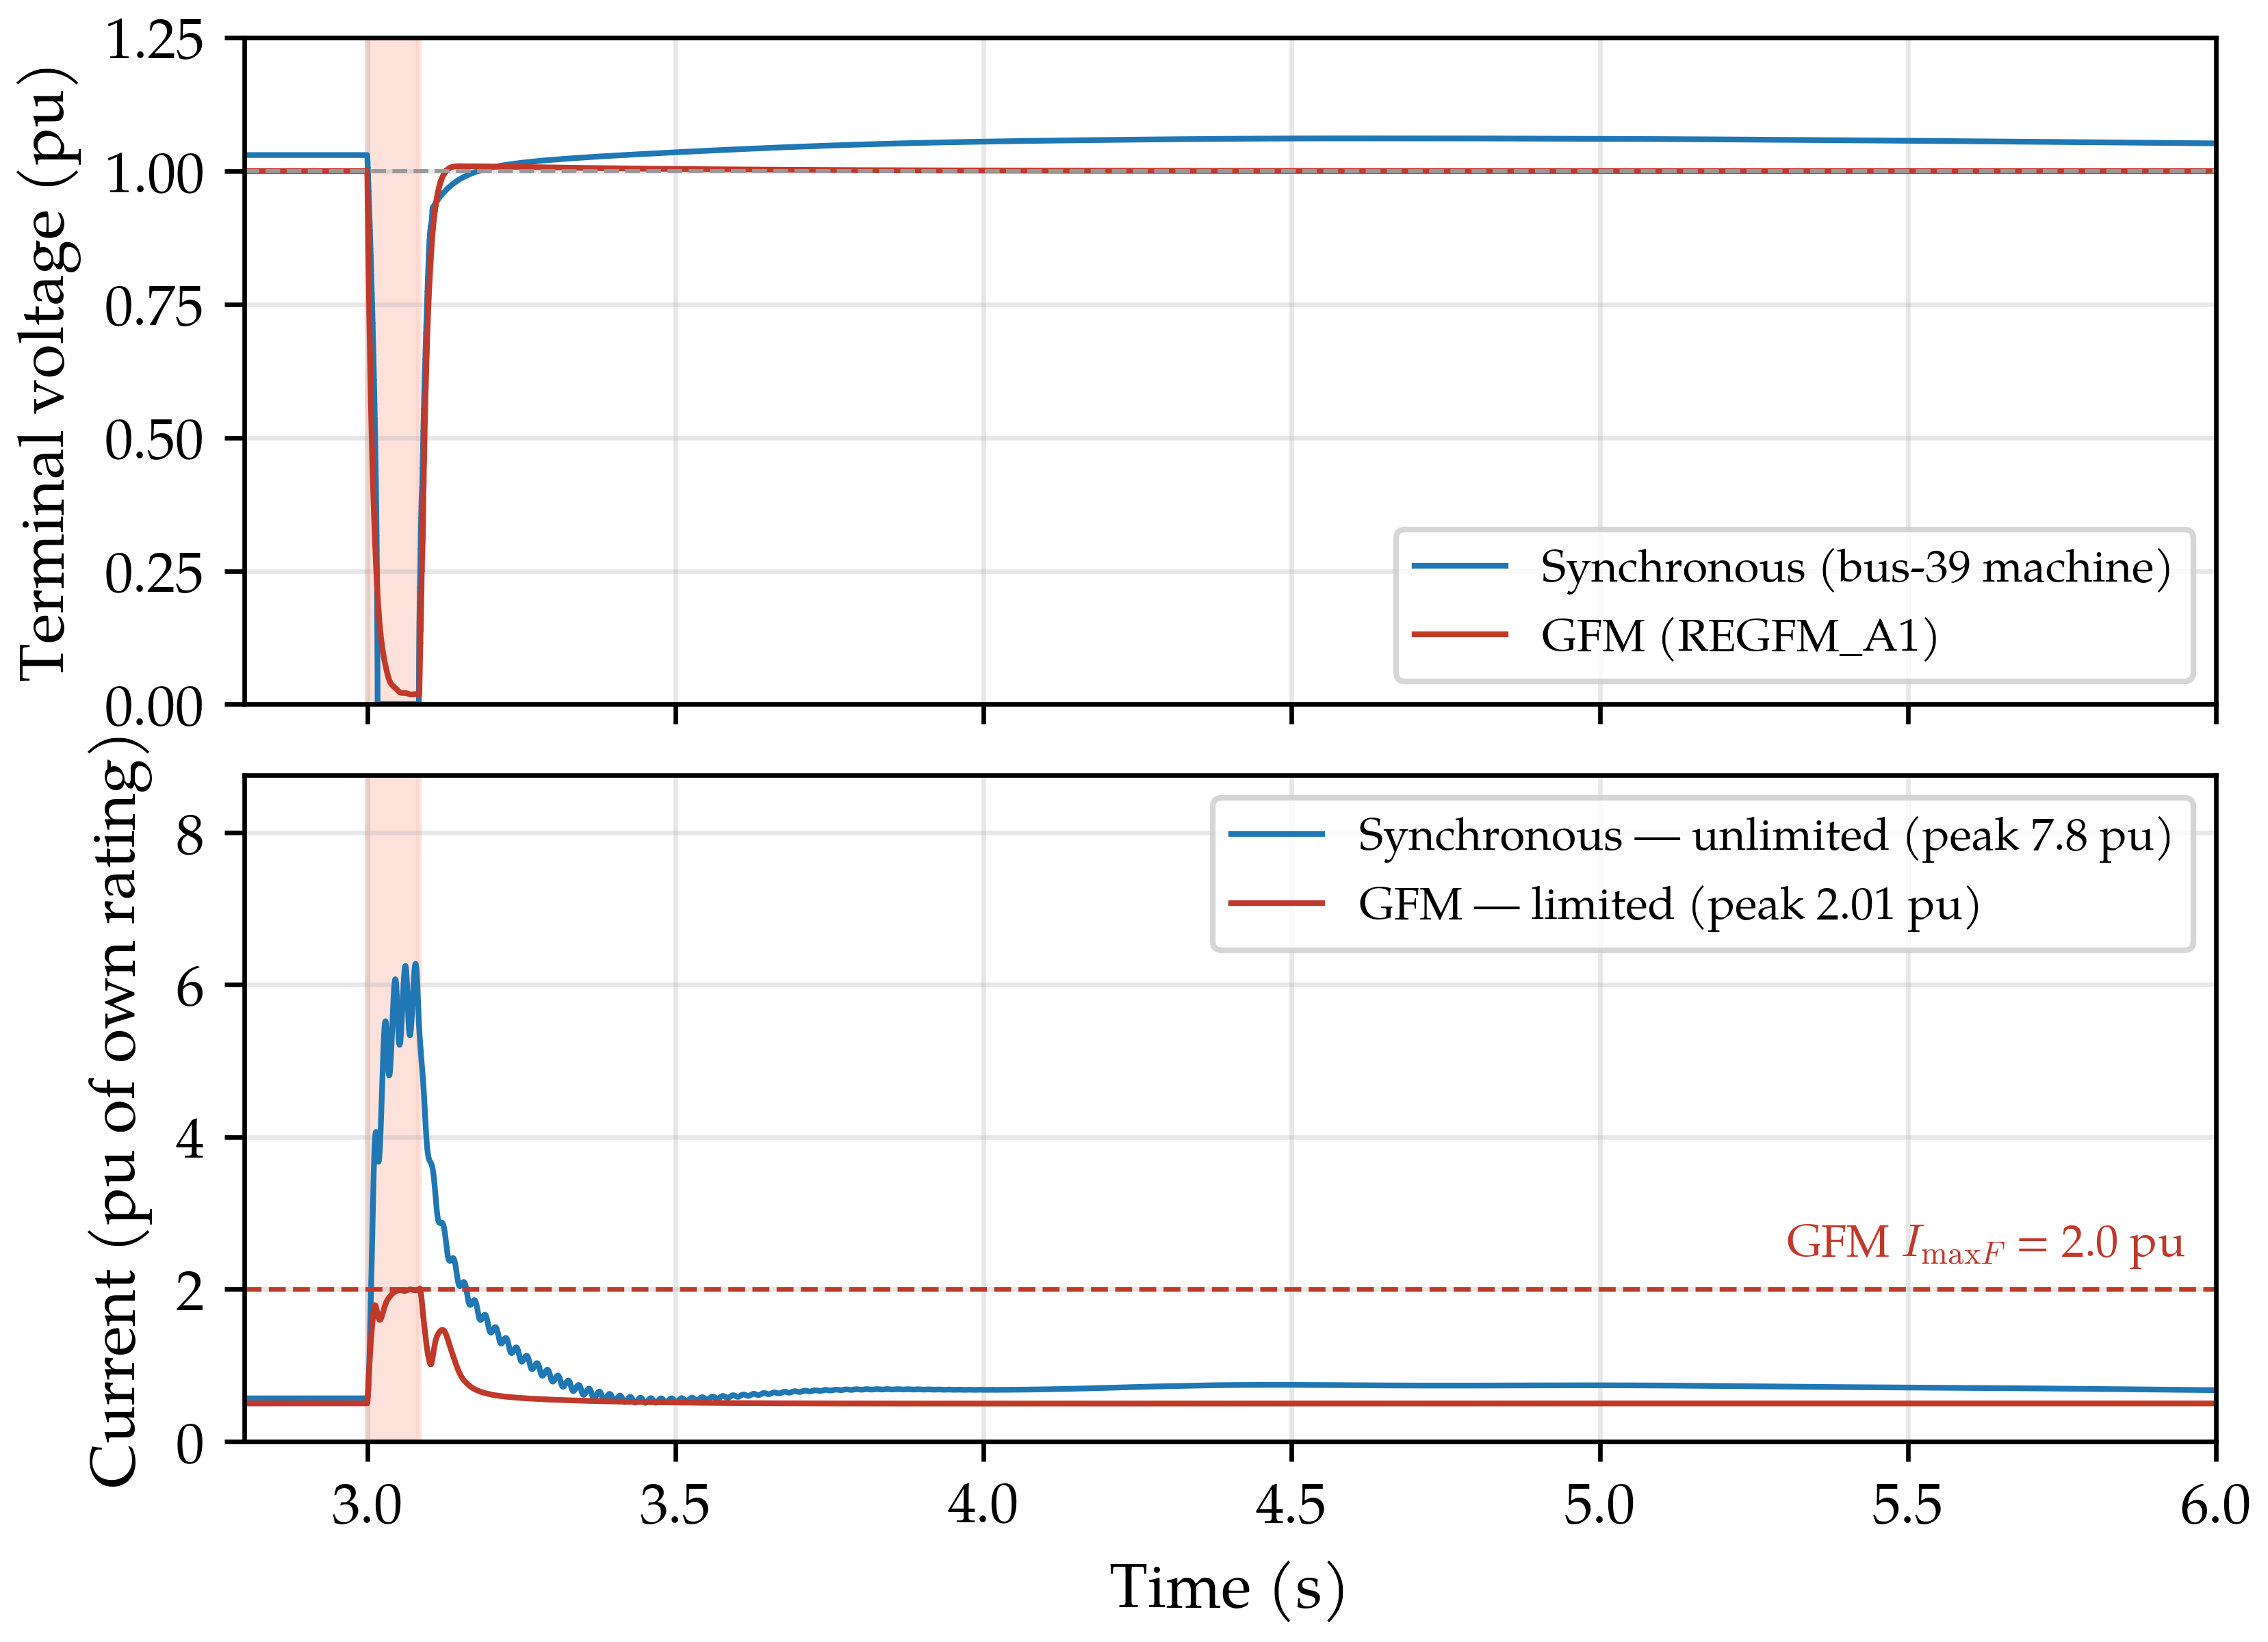
\includegraphics[width=0.85\textwidth]{fig6_smib_sync_vs_gfm_VI}
\caption{Single-device fault response: voltage and current at the device terminals for the synchronous machine and the GFM inverter (neither case has a step-up transformer), with the GFM transient-current setting at 2.0 per unit and both devices dispatched at 0.50 per unit.}
\label{fig:smibvi}
\end{figure}

\begin{figure}[tbp]\centering
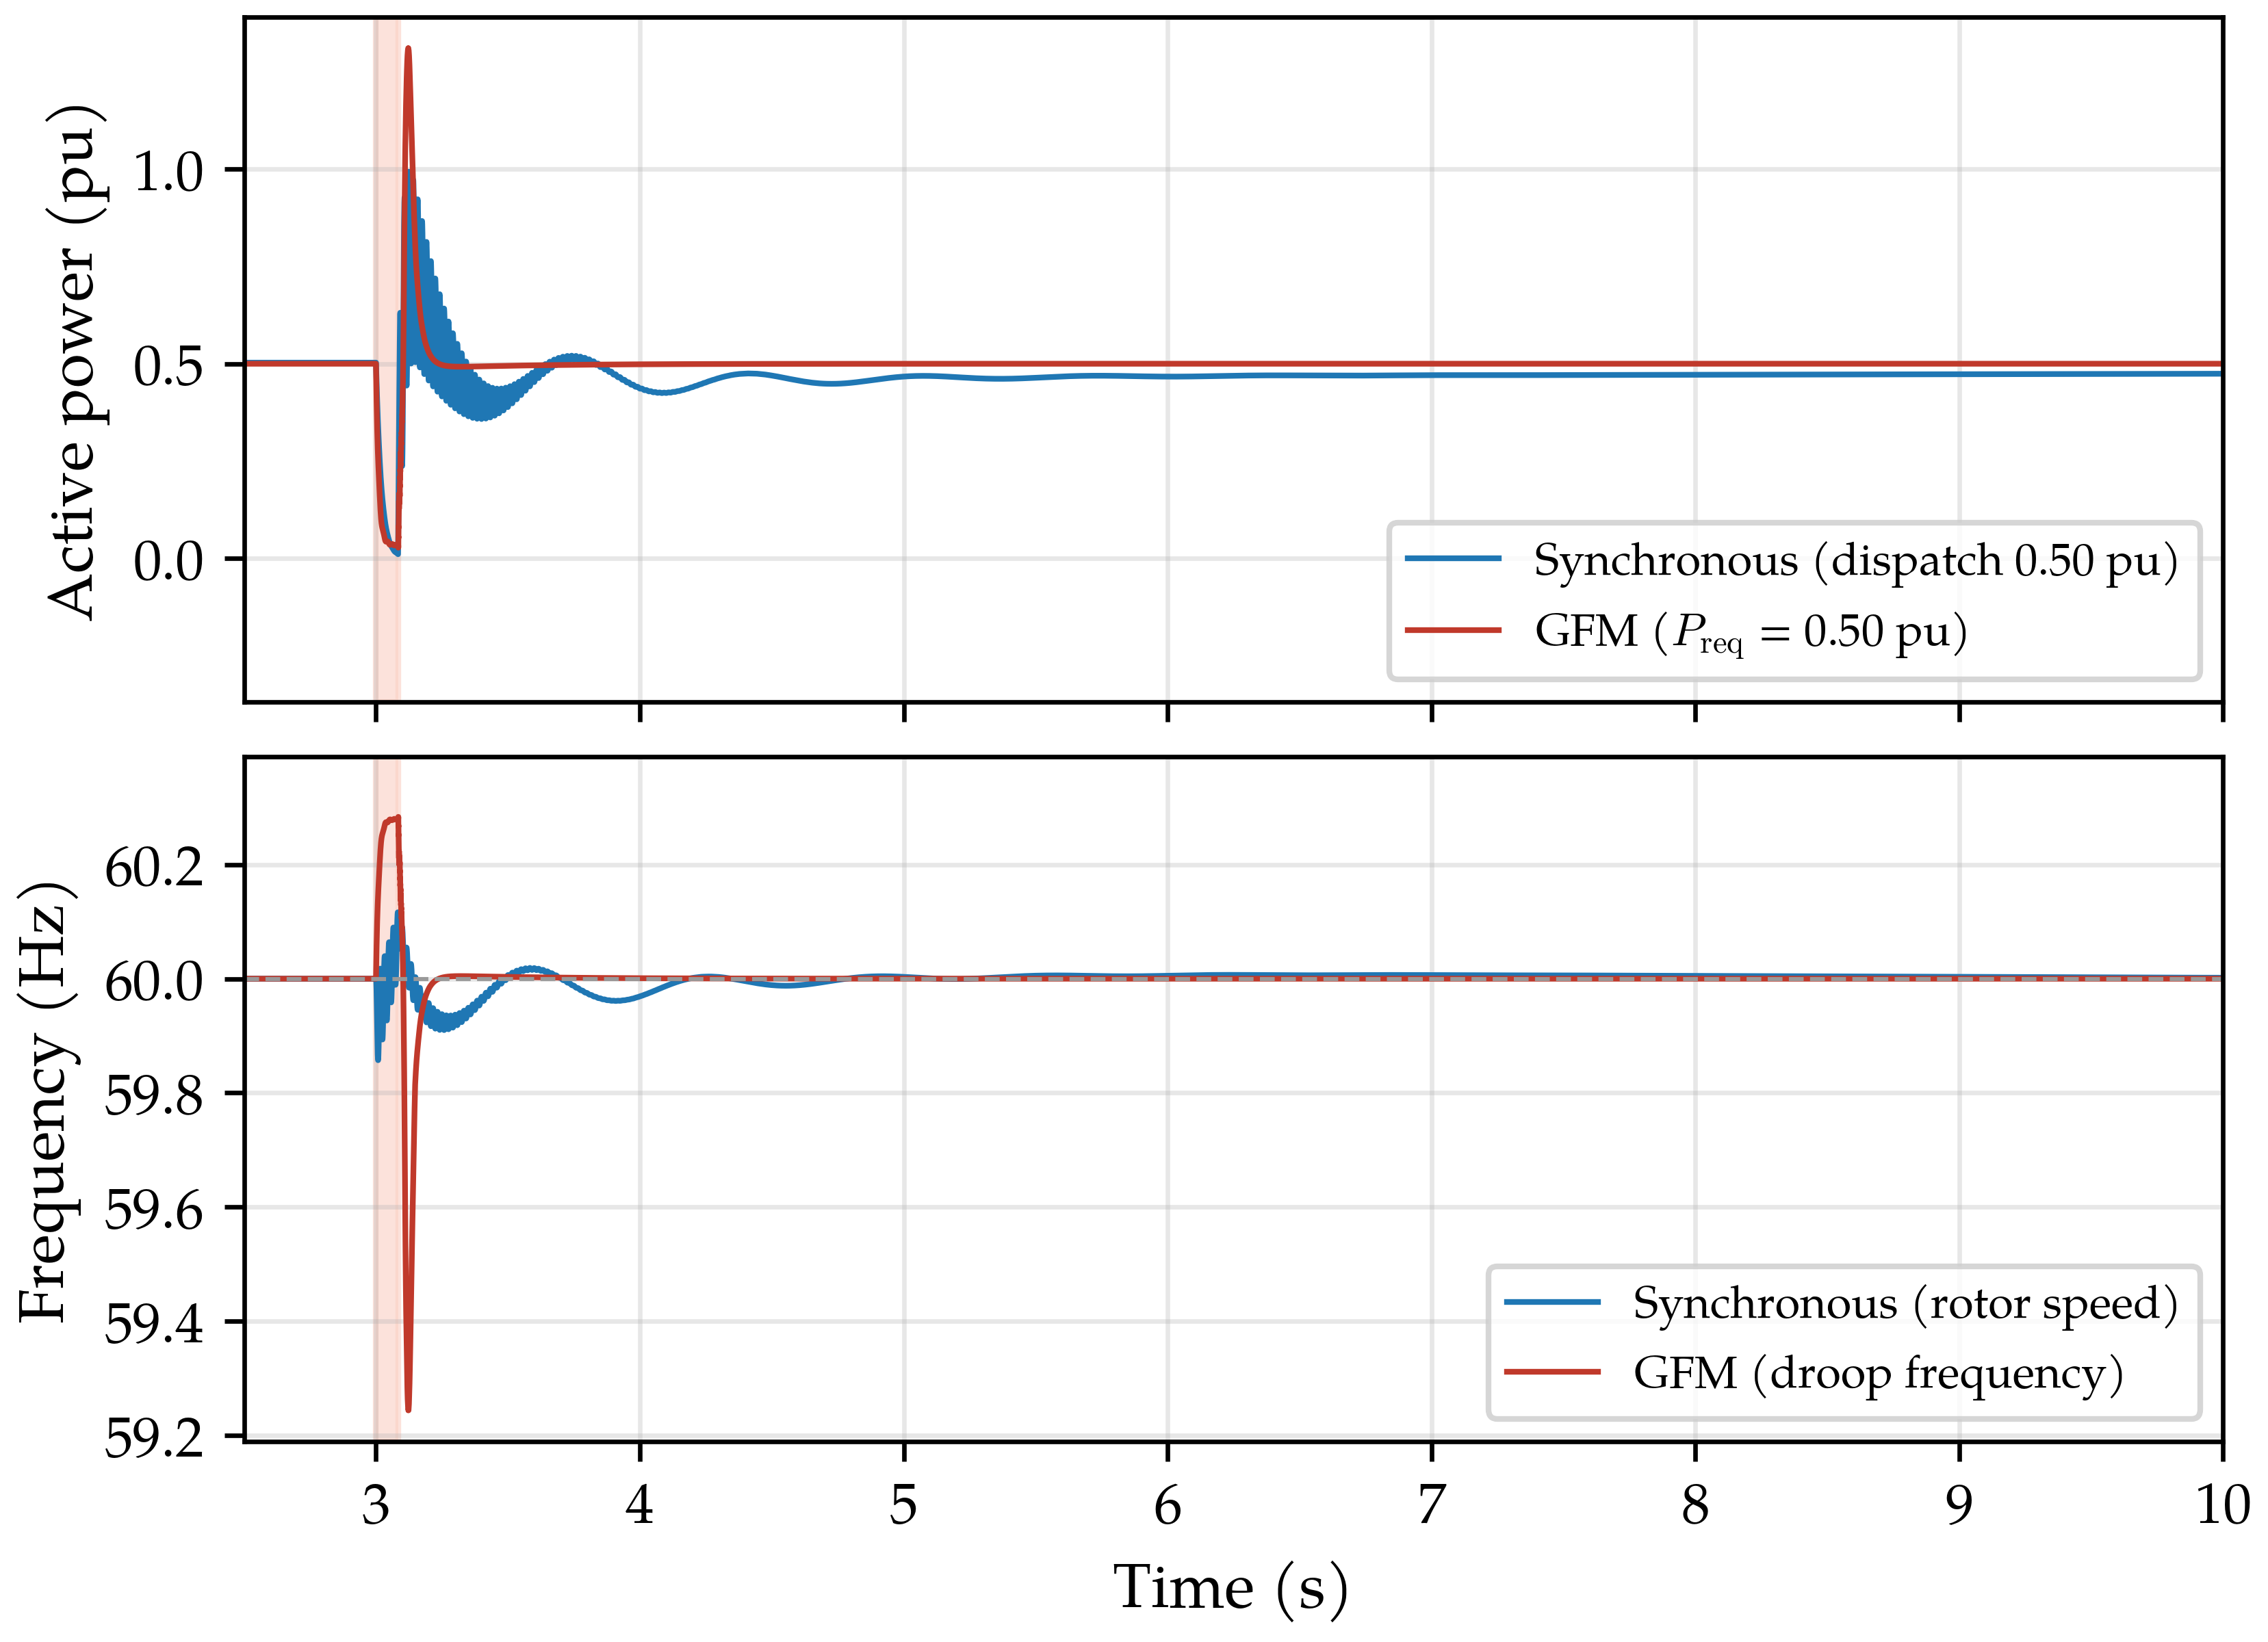
\includegraphics[width=0.85\textwidth]{narr_smib_sync_vs_gfm_Pf}
\caption{Single-device active-power and frequency responses at matched 0.50 per-unit dispatch. The dense band on the machine trace for about 0.5~s after clearing is a 60~Hz ripple of the instantaneous power calculation, produced by the direct-current offset of the armature current after the bolted fault; it decays with that offset and is not an oscillation of the machine. The machine's 1.5~Hz oscillation that follows decays at 1.6~s$^{-1}$ (Section~\ref{sec:smib}).}
\label{fig:smibpf}
\end{figure}

Figure~\ref{fig:smibipiq} separates the active and reactive current contributions. Both active powers return to 0.50 per unit; the active-current levels differ after clearing because $I_{\mathrm{P}}=P/V$ and the machine's terminal voltage settles at 1.06 per unit under its exciter while the inverter's is 1.00 per unit. The selected GFM model provides a rapid reactive-current response, 0.4--0.6 per unit through the first 50~ms after clearing. The machine response includes field-circuit dynamics: its reactive current is negative for 0.16~s after clearing, reaching $-0.65$ per unit at 3.12~s while its terminal voltage recovers from 0.95 to 1.02 per unit, and its exciter then raises the reactive power to 0.59 per unit at 1.06 per-unit voltage by 5~s. This comparison connects voltage support to device structure and controls. It does not imply identical current capabilities or response bandwidths across inverter designs.

\begin{figure}[tbp]\centering
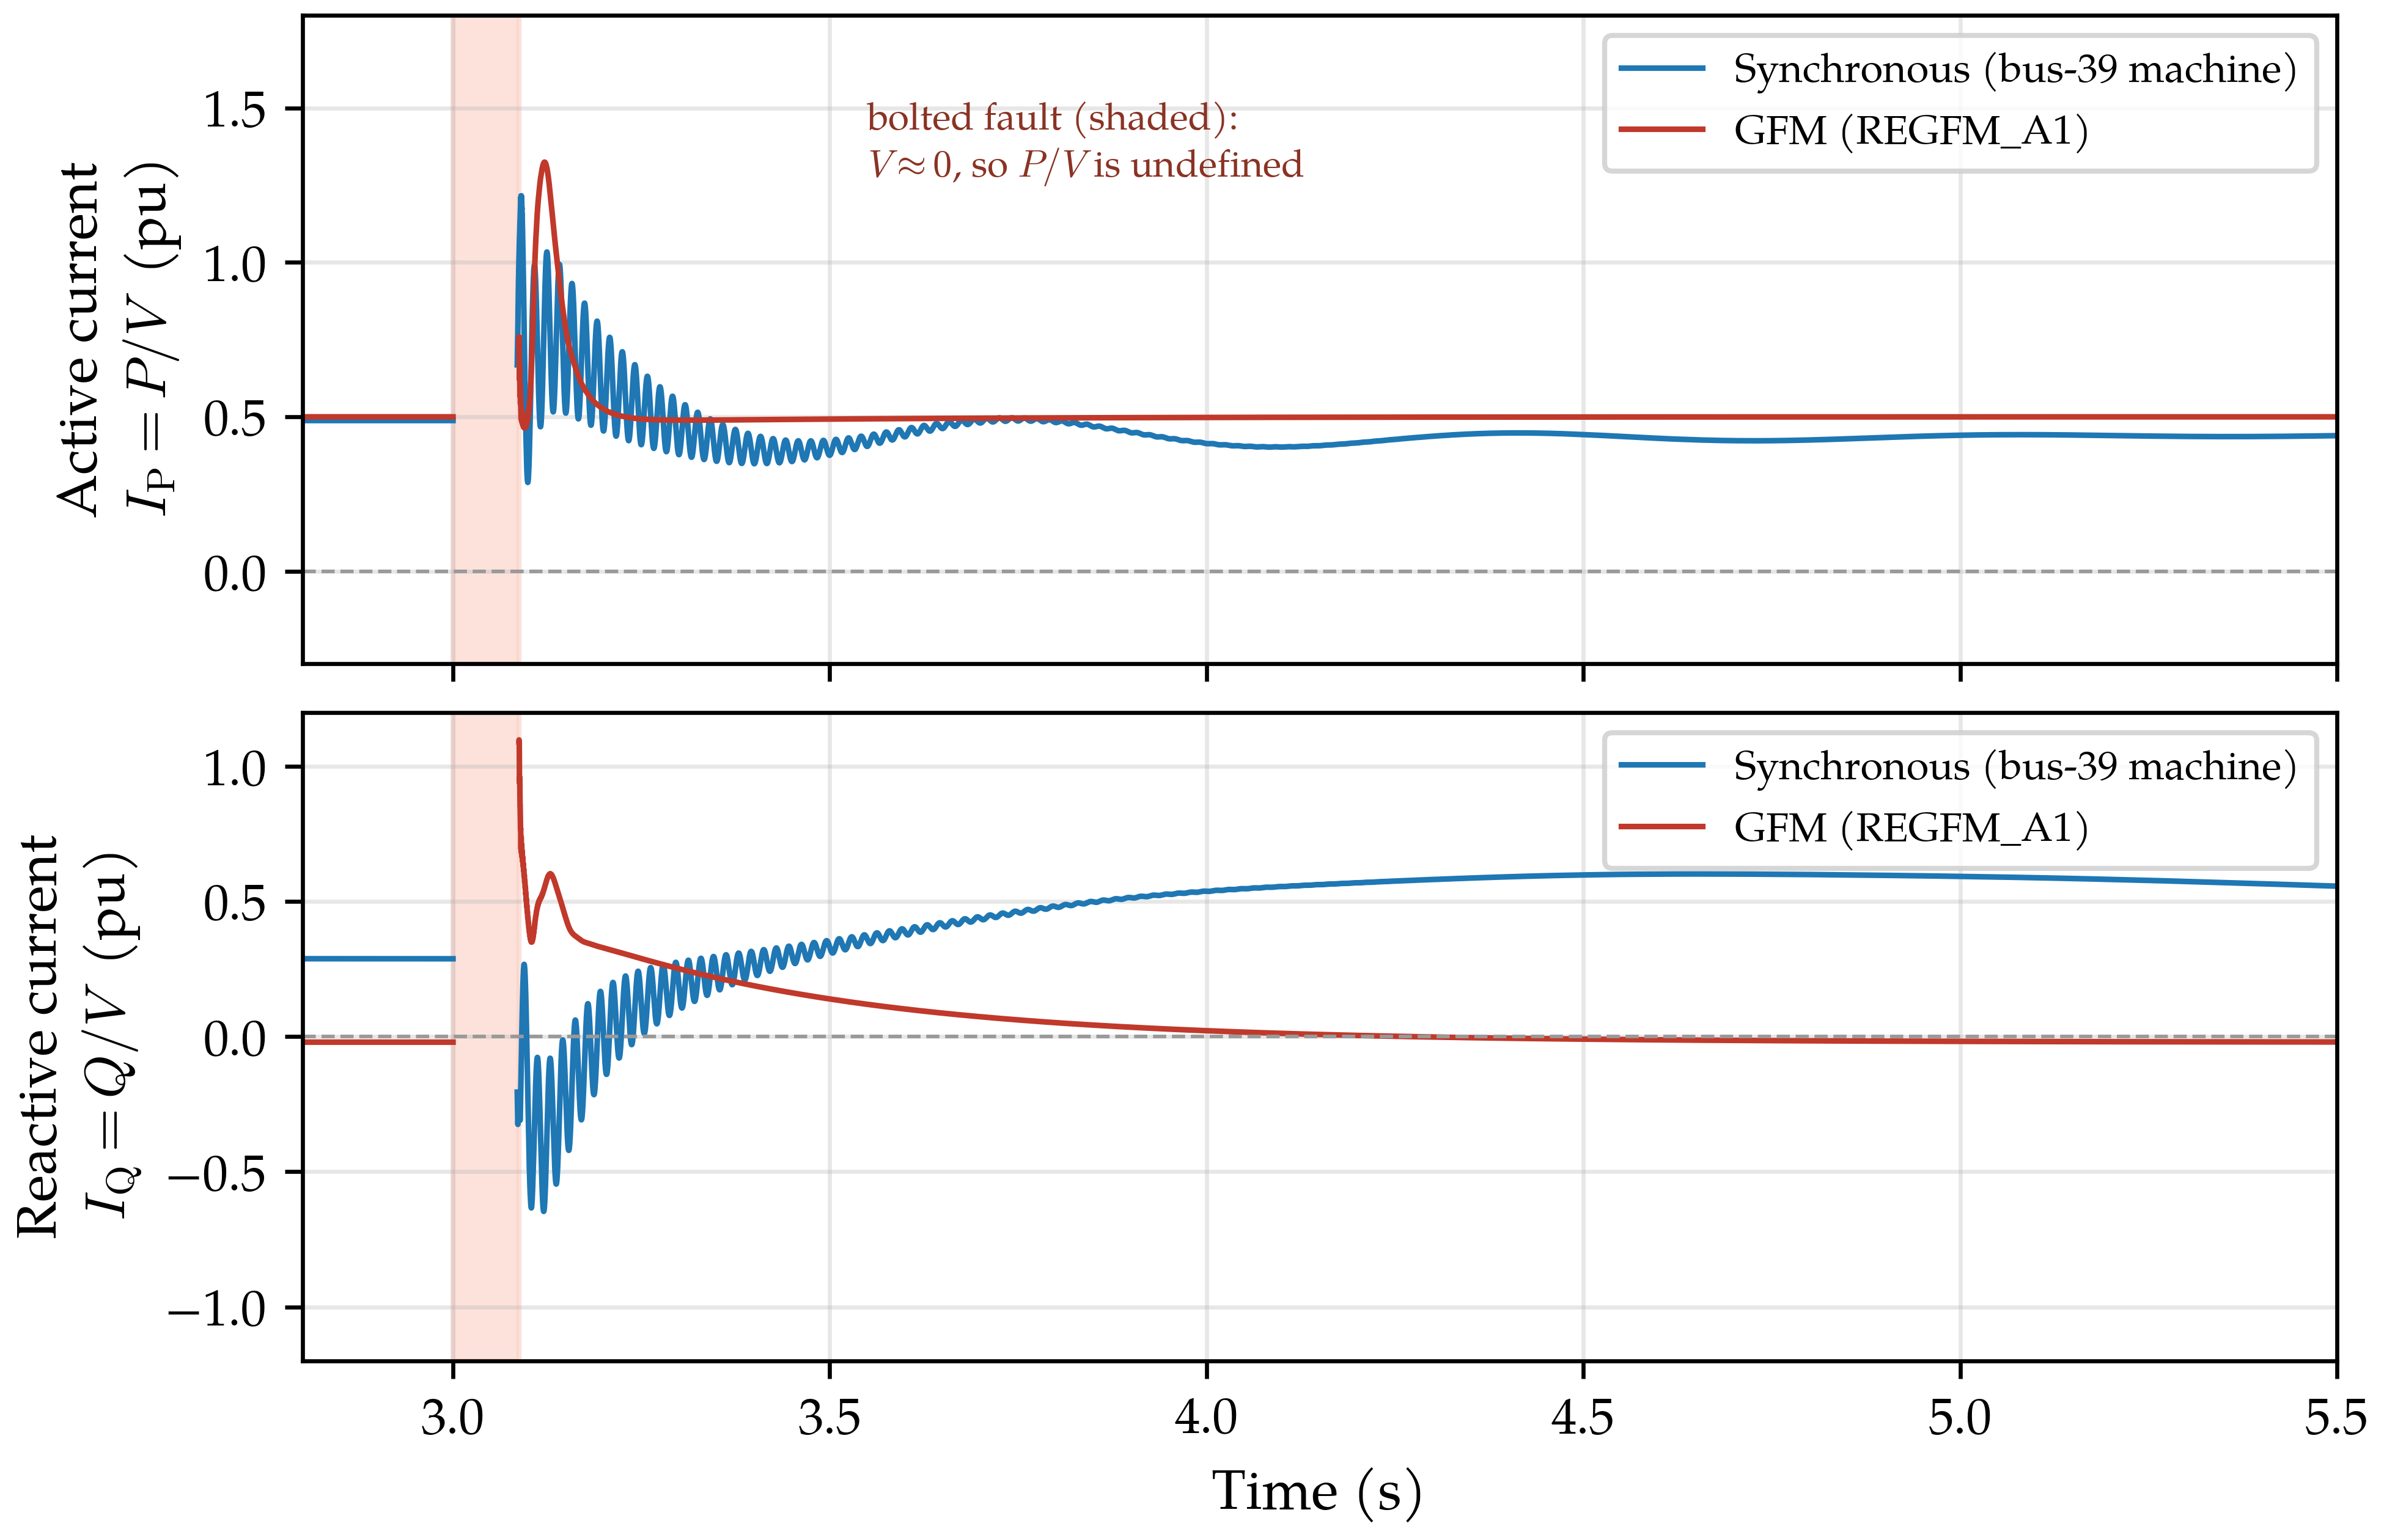
\includegraphics[width=\textwidth]{smib_IPIQ}
\caption{Active and reactive current components for the single-device fault comparison, $I_{\mathrm{P}}=P/V$ and $I_{\mathrm{Q}}=Q/V$ on each device base, positive for injection into the grid and blanked while $V<0.2$ per unit, with both devices dispatched at 0.50 per unit; the 60~Hz ripple on the machine traces is the armature direct-current offset described for Figure~\ref{fig:smibpf}.}
\label{fig:smibipiq}
\end{figure}

\subsection{Equivalent Damping, Inertia, and Settling Time}
\label{sec:dampinertia}
Both models share the swing form, so their damping coefficients can be compared directly. For small deviations of the per-unit speed, Equation~\eqref{eq:swingeq} reads
\begin{equation}
2H\,\frac{\mathrm{d}\Delta\bar{\omega}}{\mathrm{d}t}=\Delta P_{\mathrm{mech}}-\Delta P_{\mathrm{e}}-D\,\Delta\bar{\omega},
\label{eq:swinglin}
\end{equation}
where $\Delta P_{\mathrm{mech}}$ and $\Delta P_{\mathrm{e}}$ are the deviations of the mechanical and electrical power from their pre-disturbance values, and the damping term is the power that opposes the speed deviation. A device whose control changes its power in response to speed therefore contributes $D=-\Delta P/\Delta\bar{\omega}$, where $\Delta P$ is that change: the governor's change in mechanical power, $\Delta P_{\mathrm{mech}}$, for the machine, and the droop's change in output power for the inverter. $D$ is positive when the power falls as the speed rises. For a sinusoidal speed swing only the part of the power response in step with the speed acts as damping, the damping-torque component of \cite{demello1969}; the part a quarter cycle out of step is in step with the acceleration and acts as inertia.

For the inverter, Equation~\eqref{eq:heqdeq} gives $D_{\mathrm{eq}}=1/m_{\mathrm{p}}=100$ for $m_{\mathrm{p}}=0.01$, the same at every frequency within the filtered-droop model. For the machine, the governor-and-turbine path gives a frequency-dependent coefficient, the term $D+\operatorname{Re}\{G(j\Omega)\}/R_{\mathrm{SG}}$ of the synchronous-generator operator in \cite[Eq.~(50)]{chatterjee2026note}, where $G$ is the normalized response from speed deviation to mechanical power ($G(0)=1$), $R_{\mathrm{SG}}$ the permanent droop, and $\Omega=2\pi f$. Evaluated from the GGOV1 blocks of Figure~\ref{fig:controlblocks} with the Table~\ref{tab:dyr_gov_params} settings,
\begin{equation}
\frac{G(s)}{R_{\mathrm{SG}}}=-\frac{\Delta P_{\mathrm{mech}}}{\Delta\bar{\omega}}
=\frac{K_{\mathrm{turb}}\,T(s)\,\bigl[A(s)\,C(s)\,\bigl(1-2HR_{\mathrm{SG}}\,s\,F(s)\bigr)-W_{\mathrm{f0}}\bigr]}{1+R_{\mathrm{SG}}\,F(s)\,K_{\mathrm{turb}}\,T(s)\,A(s)\,C(s)},
\label{eq:govpath}
\end{equation}
where $C(s)=K_{\mathrm{pgov}}+K_{\mathrm{igov}}/s$ is the governor PI controller ($K_{\mathrm{dgov}}=0$); $A(s)=1/(1+sT_{\mathrm{act}})$ is the actuator, a first-order lag; $T(s)=(1+sT_{\mathrm{c}})/(1+sT_{\mathrm{b}})$ is the turbine lead-lag; $F(s)=1/(1+sT_{\mathrm{pelec}})$ is the first-order lag of the electrical-power measurement selected by Rselect~$=1$; and $W_{\mathrm{f0}}=W_{\mathrm{fnl}}+P_{\mathrm{m0}}/K_{\mathrm{turb}}$ is the pre-disturbance fuel flow at dispatch $P_{\mathrm{m0}}$, which enters because Flag~$=1$ makes the fuel flow the product of valve stroke and speed. The power fed back through $F(s)$ is that of a machine swinging against a stiff network, $\Delta P_{\mathrm{e}}=\Delta P_{\mathrm{mech}}-2Hs\,\Delta\bar{\omega}$, which gives the factor $(1-2HR_{\mathrm{SG}}sF)$ with $H=5.46$~s; the factor is 1 at zero frequency and $0.47-0.09j$ at 1~Hz, where it removes about half of the direct speed path. In the 39-bus fleet $\Delta P_{\mathrm{e}}$ also carries the synchronizing power exchanged with the other machines, so Equation~\eqref{eq:govpath} is the single-machine form. $D=0$ in the GENROU record.

At zero frequency the path gives $1/R_{\mathrm{SG}}=20$, so the five-to-one comparison $R_{\mathrm{SG}}/m_{\mathrm{p}}=0.05/0.01$ holds for these normalized coefficients in the steady-state limit only.

Figure~\ref{fig:damping} is an analytical estimate. It plots Equation~\eqref{eq:govpath}, evaluated from the governor and turbine constants of Table~\ref{tab:dyr_gov_params} alone, over the 0.1 to 3~Hz band of electromechanical swings for the fleet's dispatch range, $P_{\mathrm{m0}}=0.50$ to $1.00$ per unit of each machine's rating (bus~39 at 0.50, the other nine at 0.90--1.00). The governor holds speed by cutting fuel when the machine speeds up and adding fuel when it slows, so for a slow change its power change opposes the speed deviation and damps the swing; the actuator and the turbine delay that response. The coefficient starts at 20, falls as the two lags accumulate phase, crosses zero between 0.38 and 0.41~Hz, and reaches $-1.4$ to $-1.8$ at 1~Hz, the frequency of the inter-machine swing in Figure~\ref{fig:allsync}. Past the crossing the delay exceeds a quarter of the swing period, so the commanded power change arrives after the speed has reversed: mechanical power rises while the speed rises and feeds the swing. This is negative damping in the sense of \cite[Sec.~2.1, Eq.~(2.2); Sec.~12.5]{kundur1994}. The sign was confirmed in PSCAD on the single-machine case of Section~\ref{sec:smib} by modulating the infinite-bus frequency: the measured coefficient is negative from 0.5 to 2~Hz at both dispatches. The sign change needs both lags, $T_{\mathrm{act}}=0.5$~s and $T_{\mathrm{b}}=0.1$~s; a single first-order lag, the stand-in of \cite[Eq.~(51)]{chatterjee2026note}, never reaches $90^\circ$ and cannot change sign. Closing the feedback with $\Delta P_{\mathrm{e}}=\Delta P_{\mathrm{mech}}$ instead, or omitting the speed dependence of the fuel flow, moves the crossing to 0.6--0.7~Hz and the 1~Hz value to between $-1.1$ and $-2.0$ without changing the sign. Damper windings, excitation, the stabilizer, and network interactions also damp a mode, and none of them is in Equation~\eqref{eq:govpath}; PSS2B and ESST4B are active in all machine cases, and no case without the stabilizer was simulated. The inverter's coefficient, by contrast, is flat where the machine's changes sign. No simulation result enters the figure or the analytical rows of Table~\ref{tab:dh}; both follow from the device parameters.

The inertia comparison runs the other way: $T_{\mathrm{Pf}}=10$~ms and $m_{\mathrm{p}}=0.01$ give $H_{\mathrm{eq}}=0.5$~s, roughly one eleventh of the machine's 5.46~s. Table~\ref{tab:dh} collects the values. Strong equivalent damping with low equivalent inertia is consistent with the faster GFM settling.

The ring-down of the single-machine fault test (Figure~\ref{fig:smibpf}) gives the machine's total damping without reference to any control path. With $\Delta P_{\mathrm{e}}=K_{\mathrm{s}}\Delta\delta$ in Equation~\eqref{eq:swinglin}, the swing decays as $e^{-\sigma t}$ with $\sigma=D/(4H)$, and the logarithmic decrement of $n+1$ successive peaks, $\delta_{\log}=(1/n)\ln(a_{0}/a_{n})$, gives $\sigma=\delta_{\log}f_{\mathrm{d}}$ at the ring frequency $f_{\mathrm{d}}$ \cite[Sec.~2.6.3]{rao2011}. After a zero-phase 1 to 3~Hz band-pass filter, which removes the 60~Hz meter ripple and the exciter's slow recovery, the peaks of active power and of rotor speed give $\delta_{\log}=1.06$ at 1.53~Hz, hence $\sigma=1.62~\mathrm{s^{-1}}$ (damping ratio 0.17) and $D=4H\sigma\approx35$ per unit on the machine base; the maxima and minima of the two signals give 35.1 to 35.9, and a 0.5 to 5~Hz band gives $34.5\pm1.7$. This total includes the damper windings, the stabilizer, and the exciter as well as the governor path of Figure~\ref{fig:damping}, whose $-1.4$ to $-1.8$ is about 5\% of it, so the ring-down cannot resolve the governor's share. Reactive power, RMS voltage, and RMS current follow the exciter's aperiodic recovery and carry too little of the swing to evaluate. The inverter's record of the same test has no ring in any signal, as the reduced model predicts: $D_{\mathrm{eq}}=100$, $H_{\mathrm{eq}}=0.5$~s, and a coupling reactance of 0.25 per unit ($X_{\mathrm{L}}=0.15$ plus the SCR-10 source) give a damping ratio of about 1.3.

\begin{table}[tbp]\centering
\caption{Selected inertia and damping quantities: analytical values from the device parameters (Equations~\eqref{eq:heqdeq} and~\eqref{eq:govpath}), except the last row, measured from the single-device fault records. Damping coefficients use normalized power per normalized frequency.}
\label{tab:dh}
\small
\begin{tabular}{>{\raggedright\arraybackslash}p{0.45\linewidth}>{\raggedright\arraybackslash}p{0.20\linewidth}>{\raggedright\arraybackslash}p{0.24\linewidth}}\toprule
Quantity & GFM (droop) & Synchronous machine\\\midrule
Inertia constant & $H_{\mathrm{eq}}=0.5$~s & $H=5.46$~s\\
Damping coefficient, zero frequency & 100 & 20 (governor)\\
In-phase coefficient, 1~Hz & 100 & $-1.4$ to $-1.8$ (governor)\\
Governor zero crossing & Not applicable & 0.38--0.41~Hz\\
Total damping of the swing mode, from the fault ring-down ($4H\sigma$) & no ring (damping ratio above 1) & 35, at 1.5~Hz\\\bottomrule
\end{tabular}
\end{table}

\begin{figure}[tbp]\centering
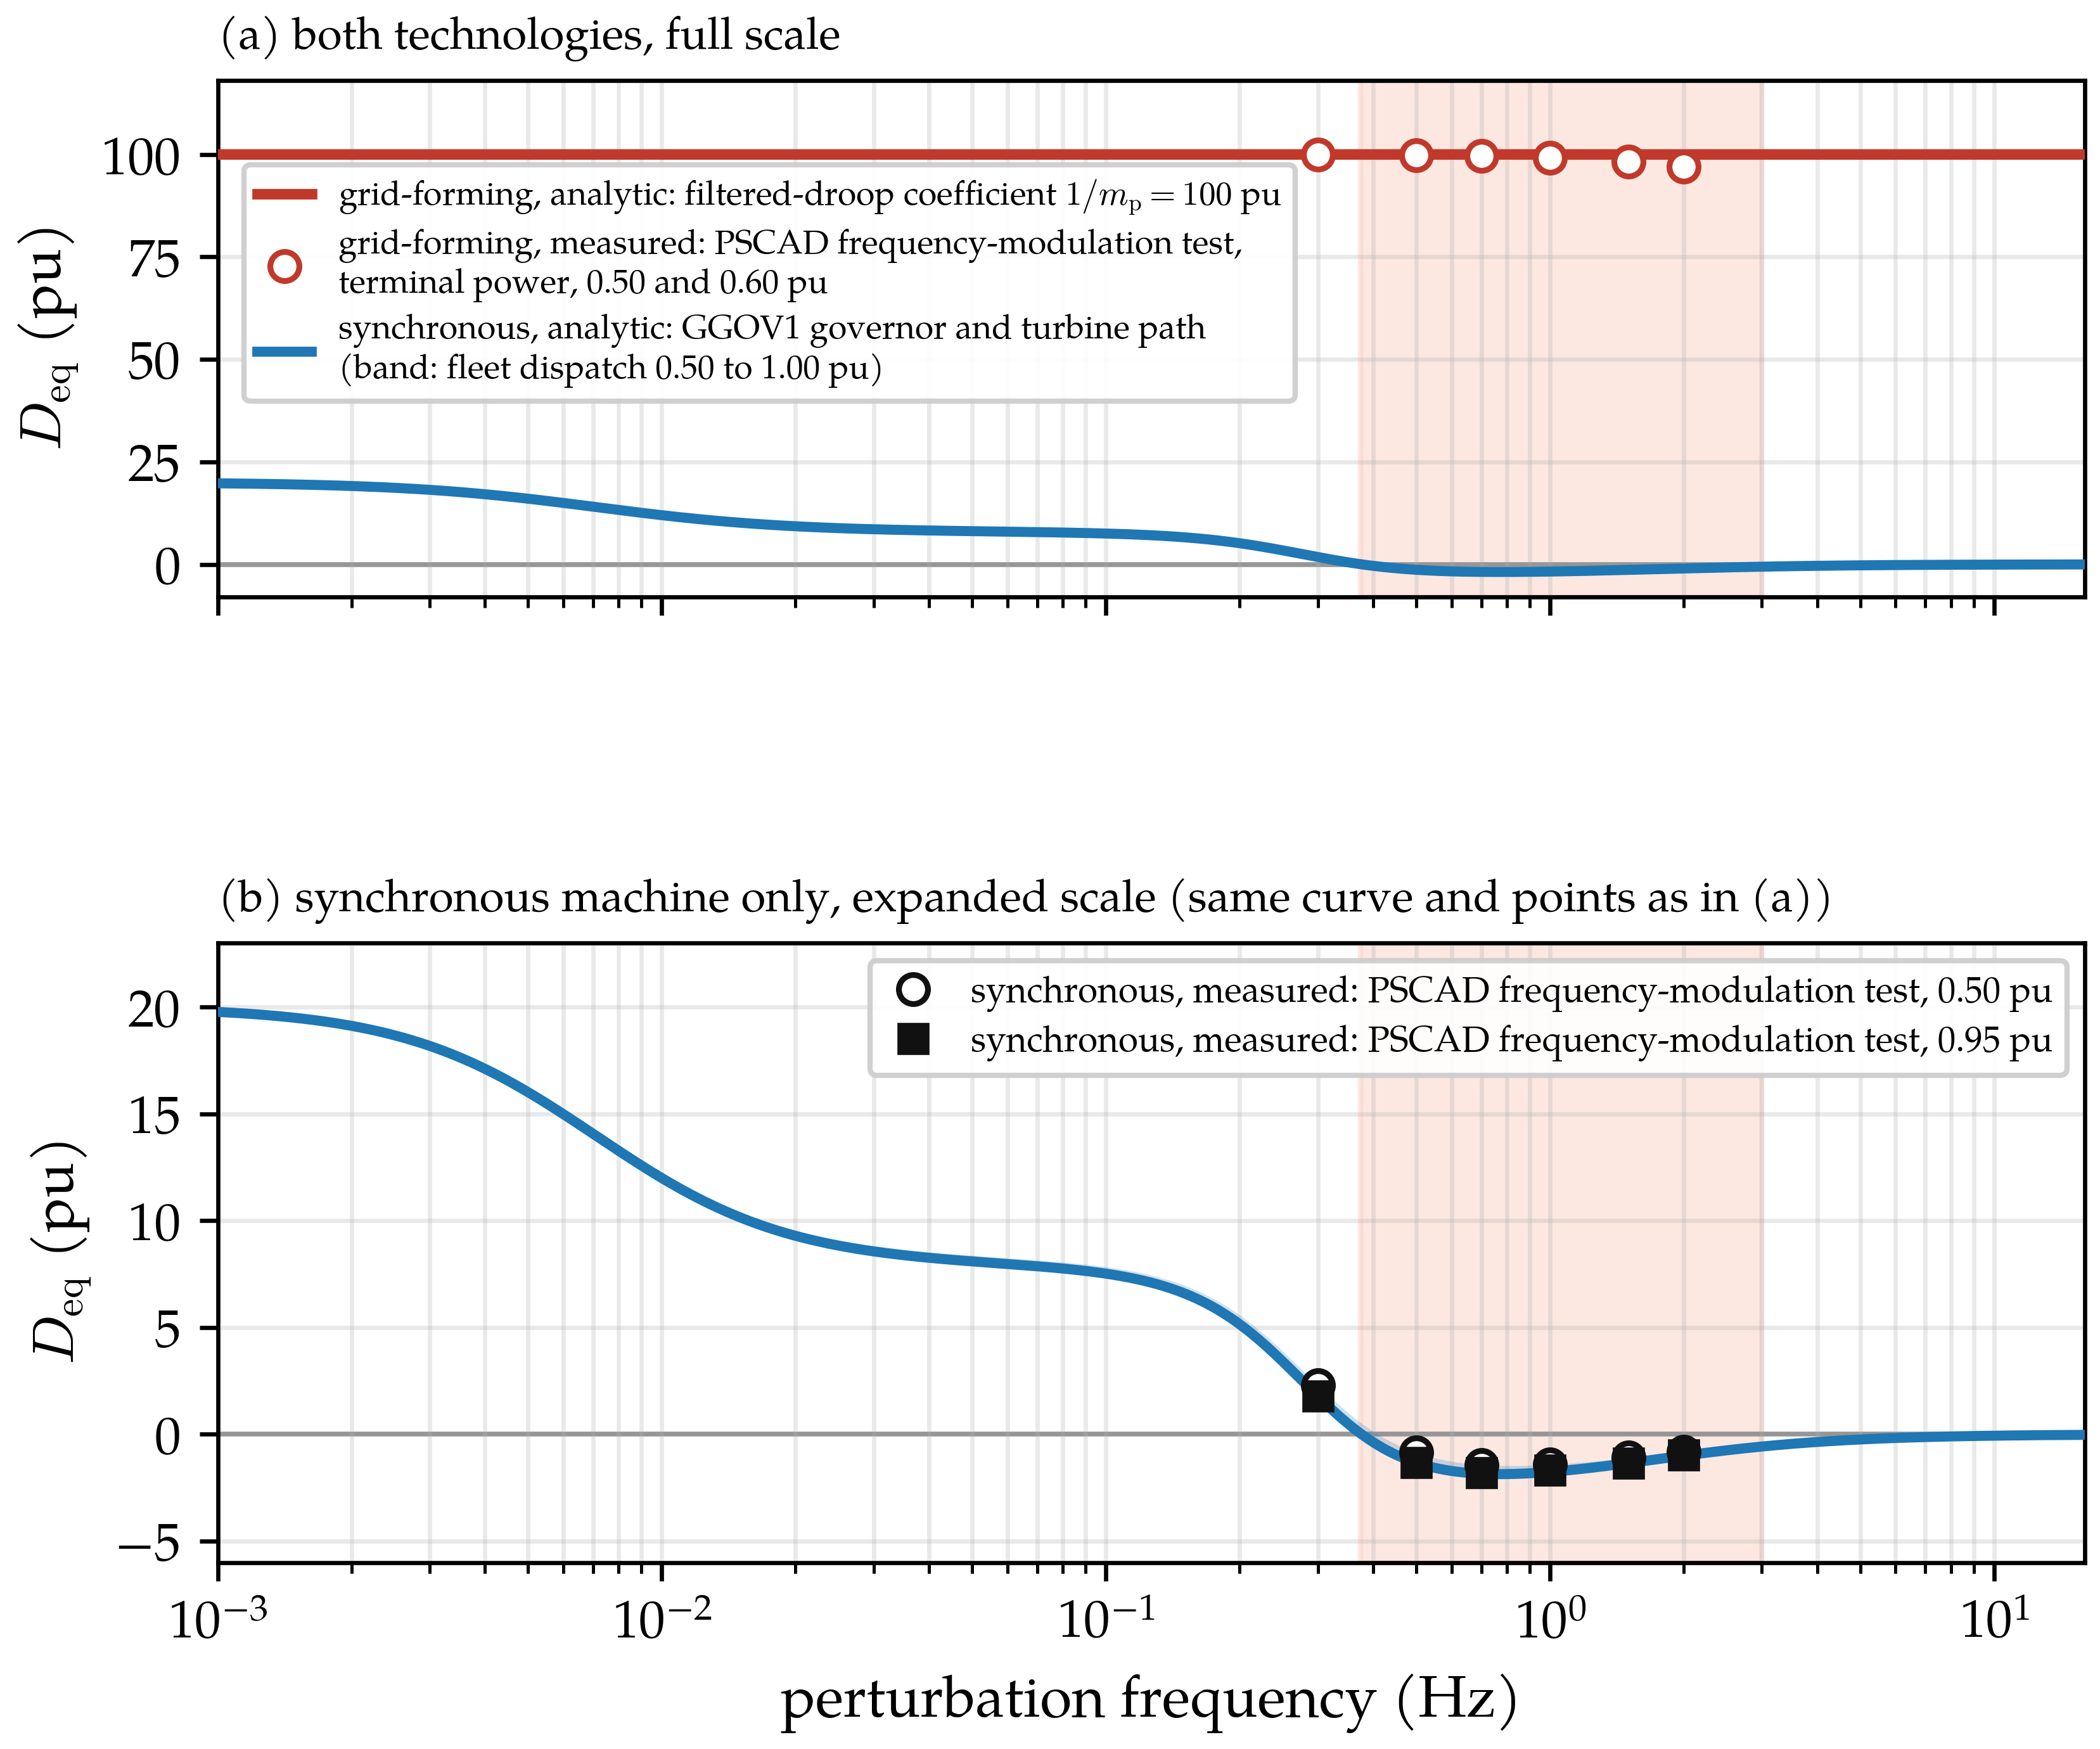
\includegraphics[width=0.85\textwidth]{narr_damping_vs_freq}
\caption{Analytical estimate of the equivalent damping versus perturbation frequency, normalized power per normalized frequency: the GFM filtered-droop coefficient $D_{\mathrm{eq}}=1/m_{\mathrm{p}}=100$ and the machine governor-and-turbine path of Equation~\eqref{eq:govpath} (band: fleet dispatch 0.50 to 1.00 per unit; line: median dispatch; shading: where the path is negative).}
\label{fig:damping}
\end{figure}

\subsection{Measuring GFM Equivalent Inertia}
\label{sec:inertiaest}
The ERCOT PMView inertia estimation test applies a frequency ramp and calculates an estimated equivalent inertia $H_{\mathrm{est}}$ from the incremental power response. We used PMView~3.5 profile~17, associated with the Dynamics Working Group Procedure Manual Revision~24, Section~3.1.5.12 \cite{pmview,dwg24}. The test uses short-circuit ratio (SCR)~3, reactance-to-resistance ratio $X/R=6$, and a $-1$~Hz/s source-frequency ramp at nominal frequency 60~Hz. The short-circuit ratio is the three-phase short-circuit apparent power of the source at the point of interconnection, without the contribution of the device under test, divided by the rating of the device \cite[Ch.~1]{nerc2017scr}:
\begin{equation}
\mathrm{SCR}=\frac{S_{\mathrm{SC}}}{P_{\mathrm{rated}}},\qquad
S_{\mathrm{SC}}=\frac{V_{\mathrm{LL}}^{2}}{X_{\mathrm{g}}},\qquad
R_{\mathrm{g}}=\frac{X_{\mathrm{g}}}{X/R},
\label{eq:scr}
\end{equation}
where $V_{\mathrm{LL}}$ is the nominal line-to-line voltage at the point of interconnection and $X_{\mathrm{g}}$ and $R_{\mathrm{g}}$ are the series reactance and resistance of the PMView source, which the harness sets from the SCR and $X/R$ of the test profile \cite{pmview}. The inverter runs use $P_{\mathrm{rated}}=0.9$~MW at 0.48~kV; the harness records $S_{\mathrm{SC}}=1.8$~MVA and $X_{\mathrm{g}}=0.128~\Omega$ at SCR~2, and 36~MVA and $0.0064~\Omega$ at SCR~40. Over the 0.5~s integration window,
\begin{equation}
H_{\mathrm{est}}=60\Delta E,\qquad
\Delta E=\int_0^T(p-p_0)\,\mathrm{d}t,\qquad T=0.5~\mathrm{s},
\label{eq:agsesr}
\end{equation}
where $p_0$ is pre-disturbance power and positive incremental power denotes additional injection. Normalized power must use the same base as the inertia comparison; $\Delta E$ and $H_{\mathrm{est}}$ then have units of seconds. The imposed source frequency and the inverter's internal frequency need not coincide during the network transient.

For the synchronous-machine case, the test gives $H_{\mathrm{est}}=5.20$~s against the configured inertia of 5.46~s, a difference of $-4.8\%$. For the GFM case, it gives 7.44~s against the filtered-droop equivalent inertia of 0.5~s, approximately fourteen times larger. Figures~\ref{fig:hsync} and~\ref{fig:hgfm} show these responses. Increasing SCR from 3 to 20 raises the GFM estimate to 10.06~s without changing the configured droop parameters.

The damping contribution explains why the integrated estimate should not automatically be identified with equivalent inertia. Under the unsaturated swing-form model, assume that internal frequency follows the imposed constant ramp over the integration window. With $\Delta f(t)=\dot f\,t$, $\dot f=-1$~Hz/s, and $f_{\mathrm{n}}=60$~Hz, the incremental response is
\begin{equation}
\Delta p(t)=-\frac{2H}{f_{\mathrm{n}}}\dot f-\frac{D}{f_{\mathrm{n}}}\dot f\,t.
\label{eq:dpsplit}
\end{equation}
Integration gives
\begin{equation}
\Delta E=-\frac{2H}{f_{\mathrm{n}}}\dot f\,T-\frac{D}{2f_{\mathrm{n}}}\dot f\,T^2.
\label{eq:esplit}
\end{equation}
For a different window under the same ramp, the estimator multiplier scales from 60 to $30/T$, with $T$ in seconds. Consequently,
\begin{equation}
\boxed{H_{\mathrm{est}}=H+\frac{DT}{4}=H+\frac{T}{4m_{\mathrm{p}}}.}
\label{eq:hest}
\end{equation}
The last equality uses the filtered-droop damping coefficient, with $H=H_{\mathrm{eq}}$.

The inertia term depends on how quickly frequency changes, whereas the damping term depends on how far frequency has moved from nominal. A constant ramp therefore produces different time dependences even though both contributions appear in the same active-power trace. Integrating that trace without separating the contributions assigns both to the inertia estimate. The distinction is between interpreting the test result and changing the configured device inertia, not between a resource with energy and one without energy.

The additional term shows that damping-related power contributes to the inertia estimate over a finite integration window. Figure~\ref{fig:esplit} illustrates the constant inertial contribution as a rectangle and the accumulating damping contribution as a triangle. A longer window therefore increases the estimate even when device parameters remain unchanged. This reduced expression contains no network-strength dependence and does not, by itself, explain the SCR variation.

\begin{figure}[tbp]\centering
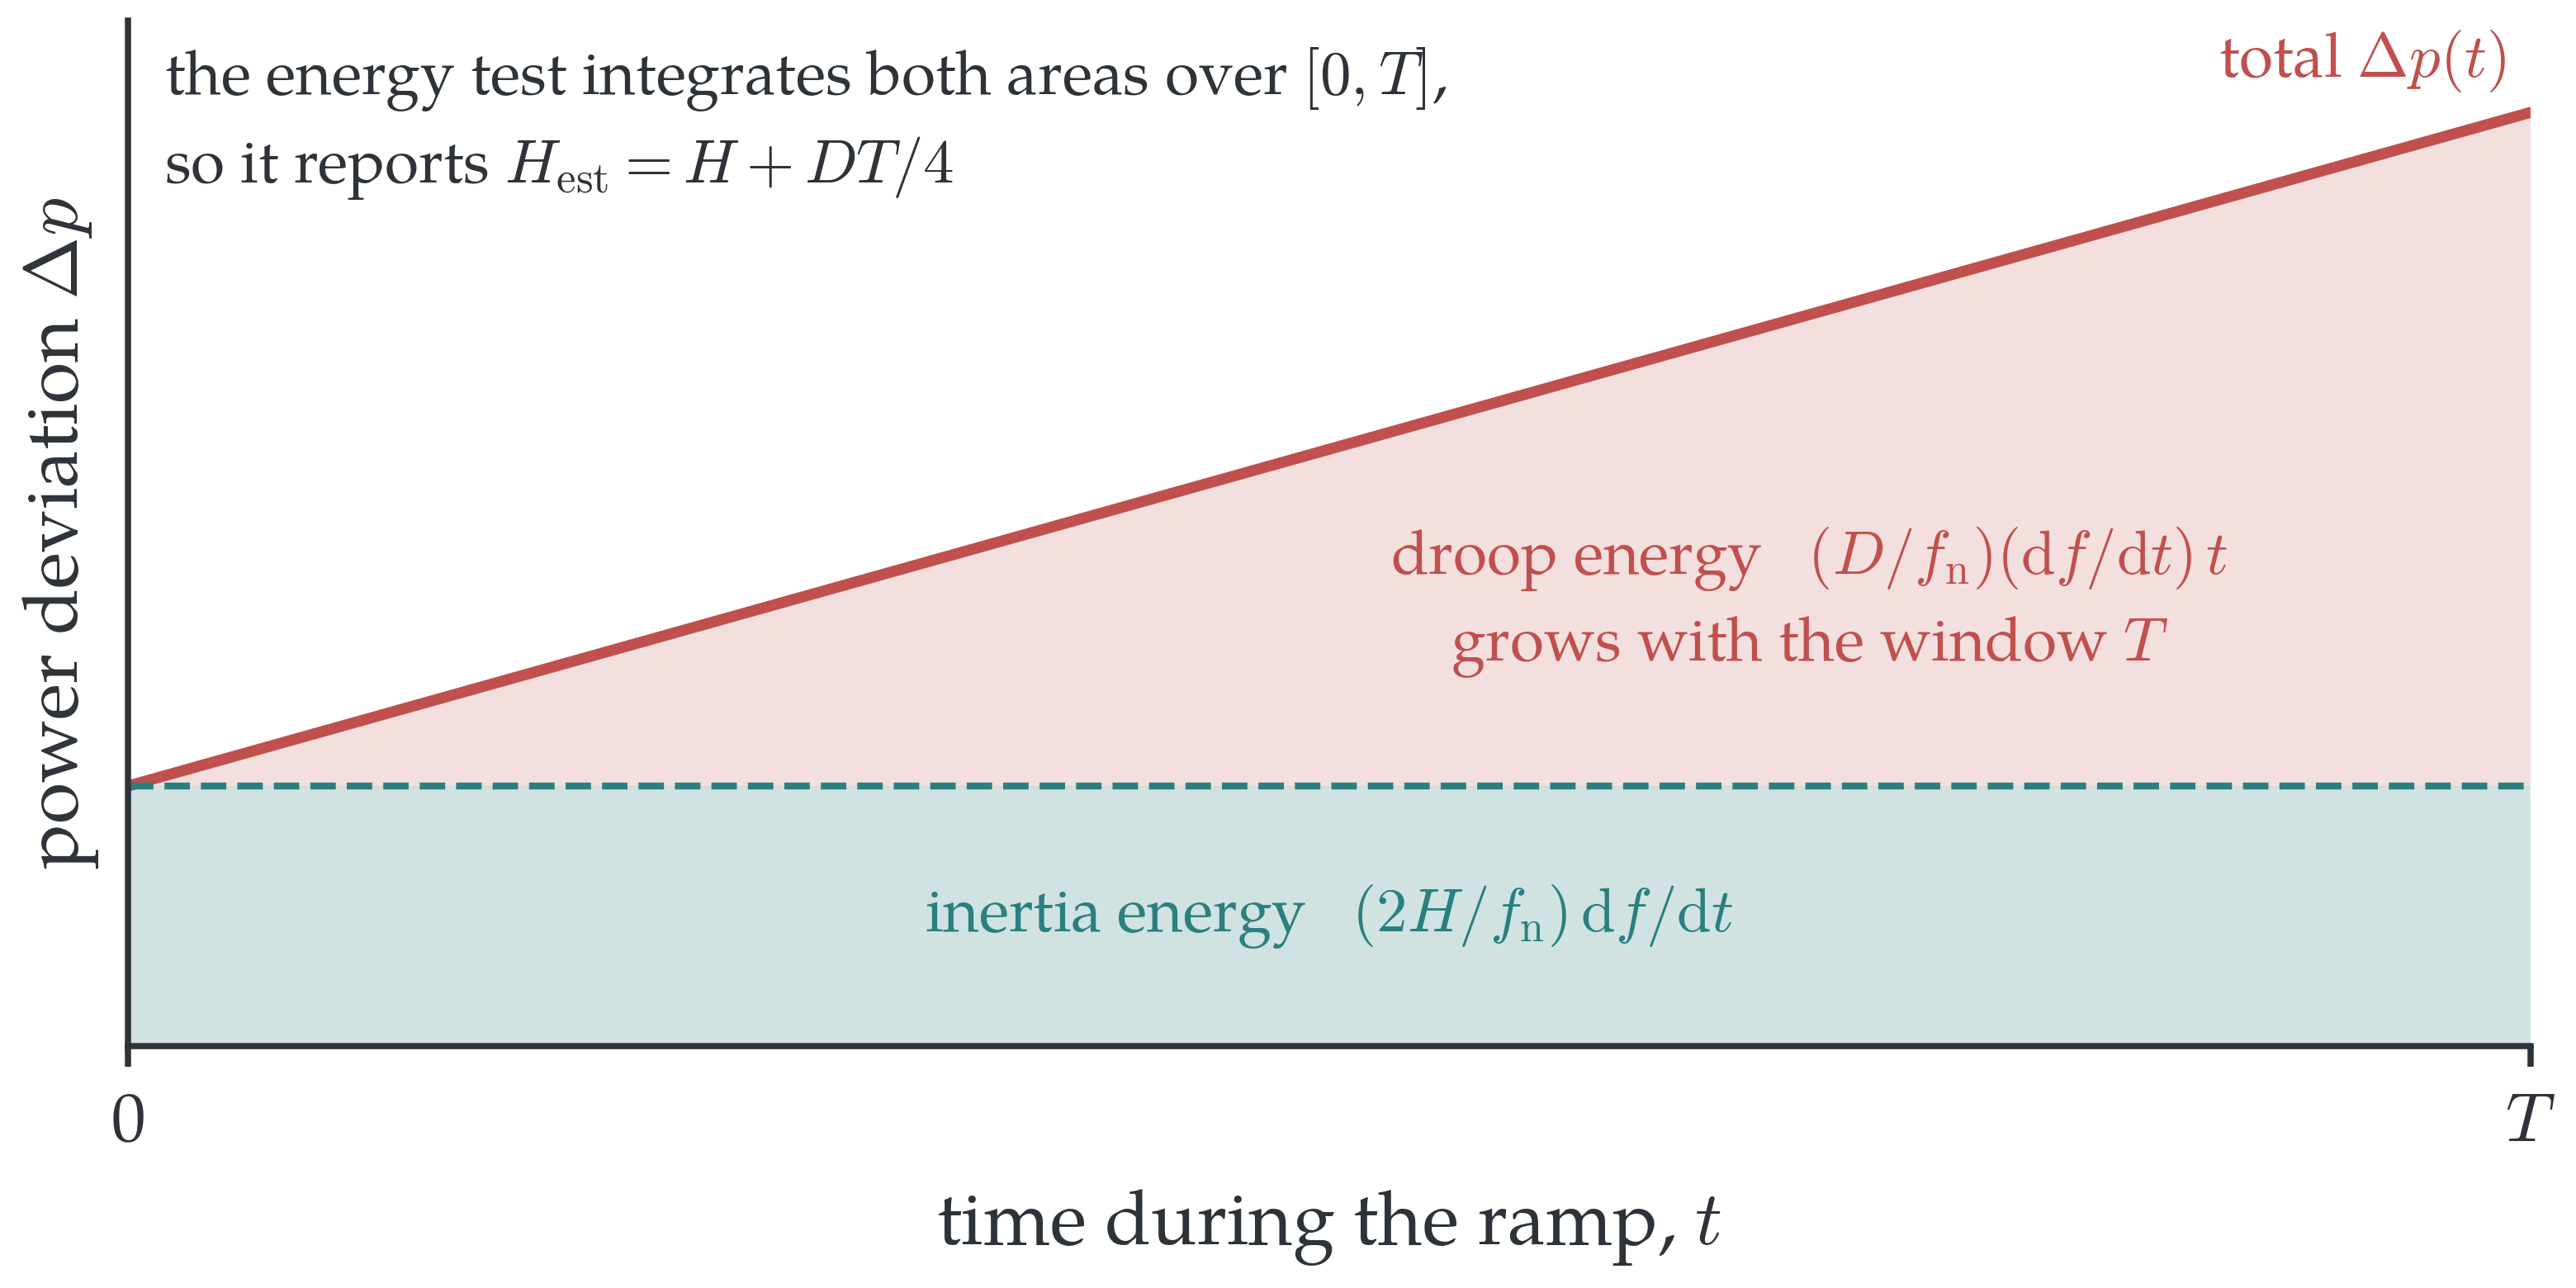
\includegraphics[width=0.8\textwidth]{inertia_energy_split}
\caption{Contributions to the integrated power response during a constant rate-of-change-of-frequency ramp, from Equations~\eqref{eq:dpsplit} and~\eqref{eq:esplit}: the inertial contribution is constant and forms a rectangle, and the damping contribution accumulates and forms a triangle.}
\label{fig:esplit}
\end{figure}

The machine and inverter also differ in response timescales. The inverter's 10~ms power filter allows droop response to develop within the half-second window, whereas turbine and governor dynamics delay the machine's contribution. Figure~\ref{fig:tscale} illustrates that distinction. The machine estimate is close to configured inertia in this test, but its finite-window response need not be purely inertial.

\begin{figure}[tbp]\centering
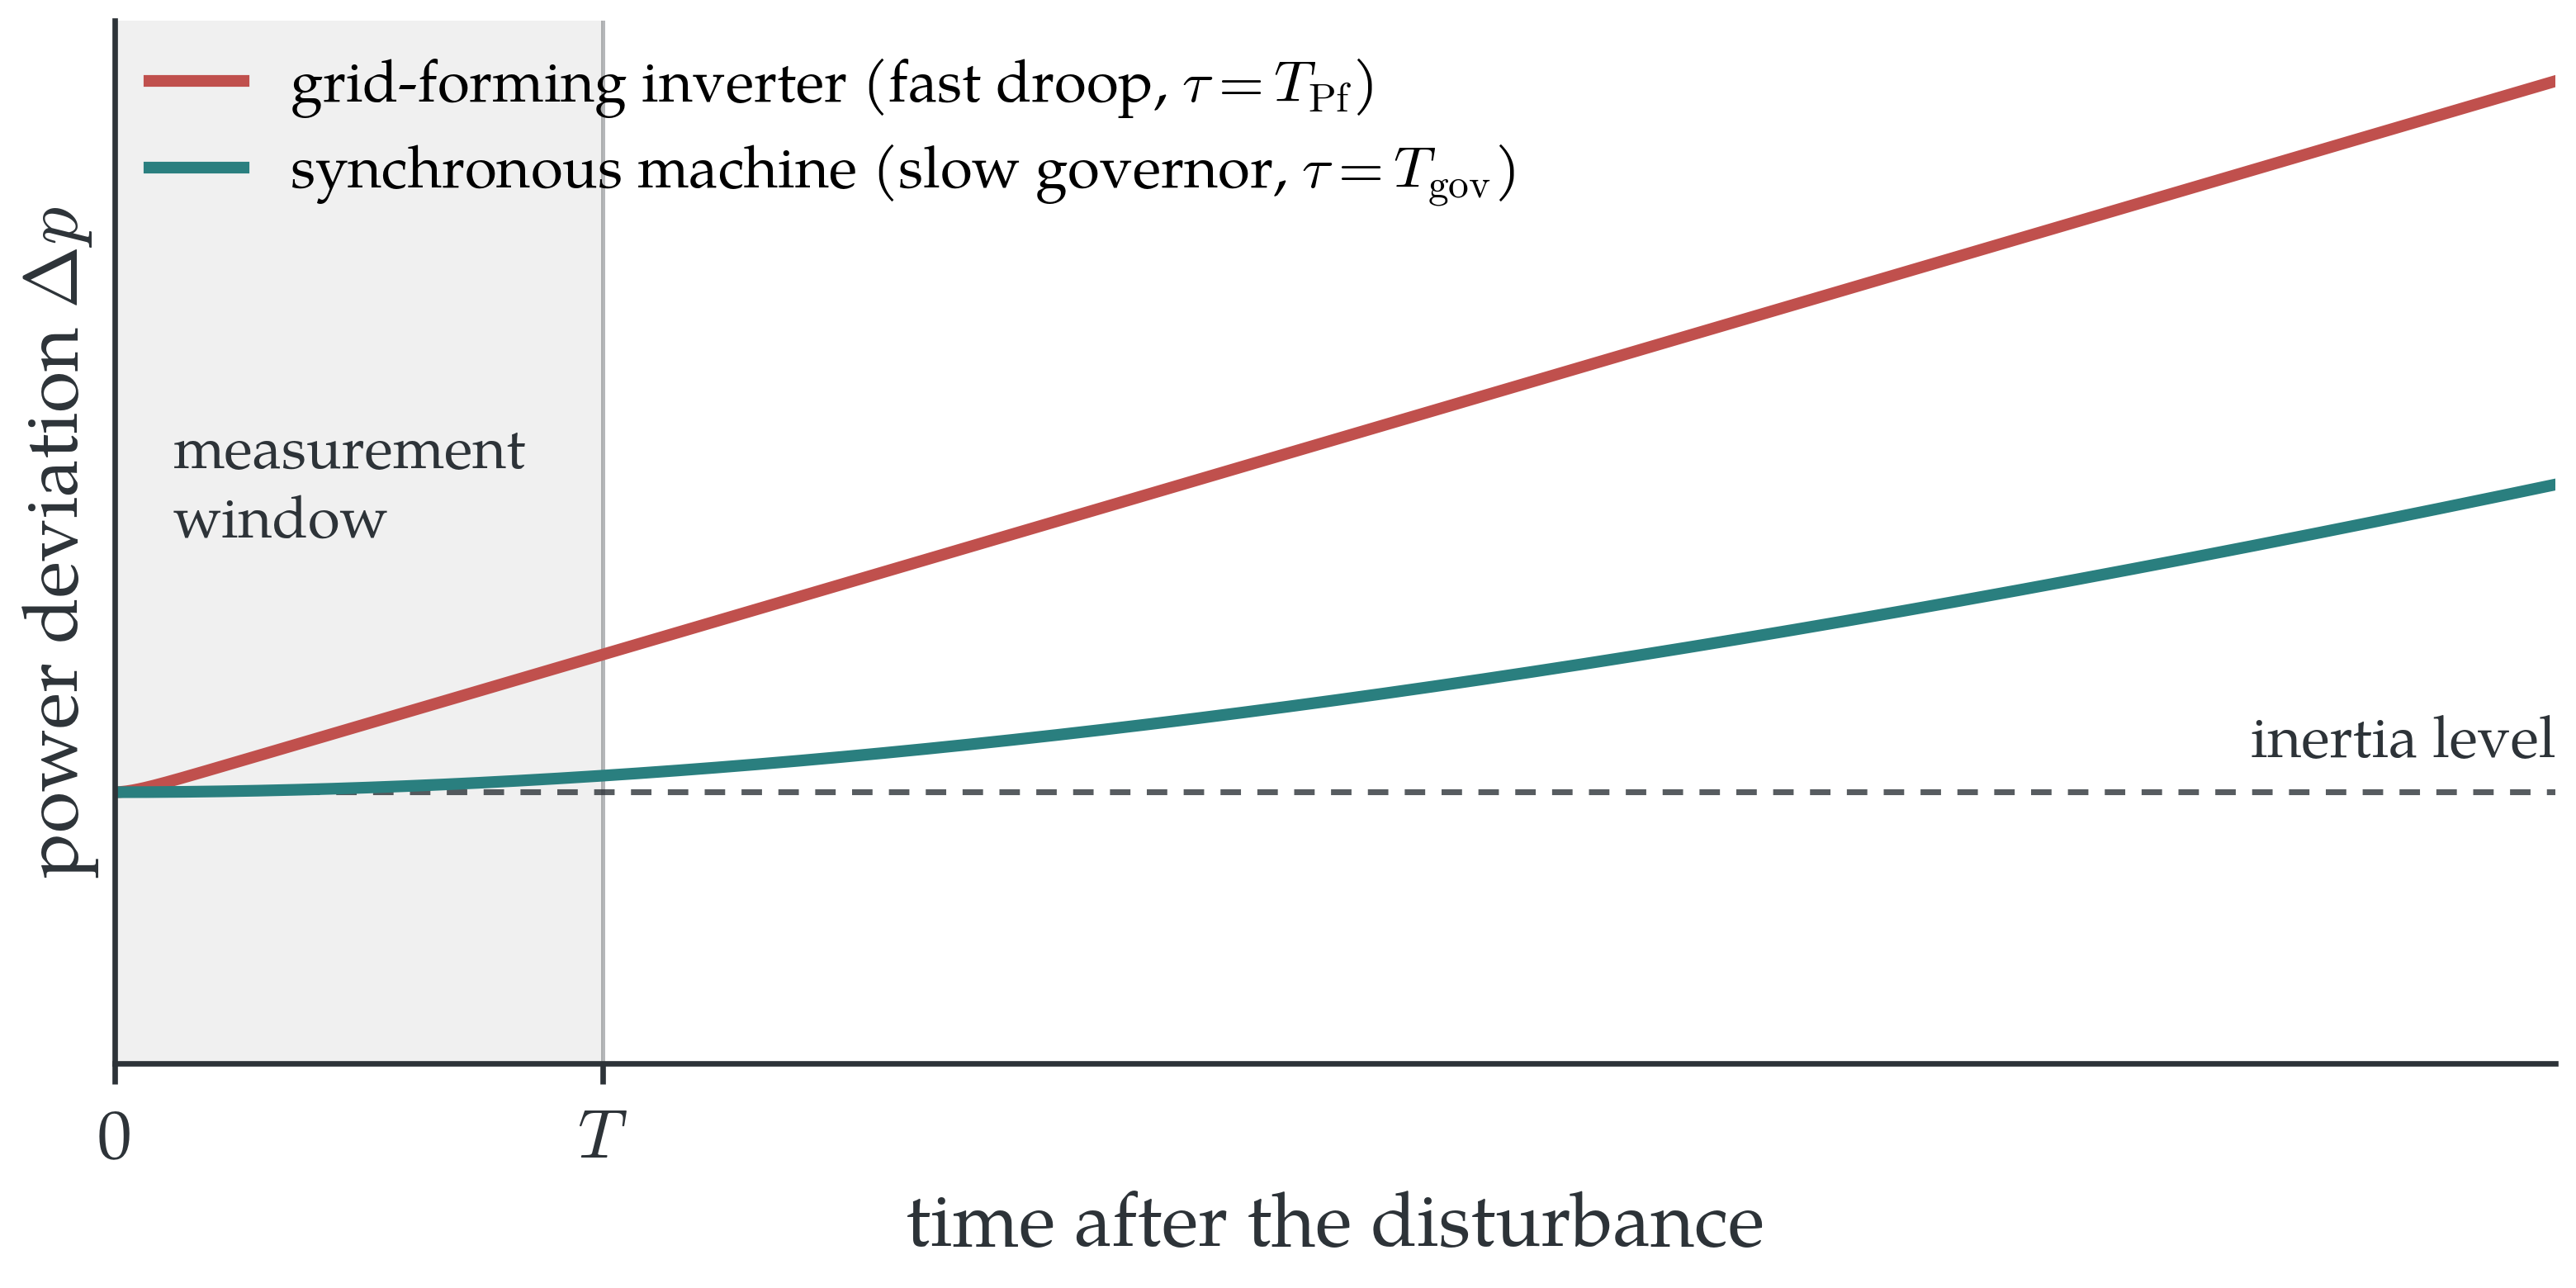
\includegraphics[width=0.8\textwidth]{inertia_timescale}
\caption{Illustrative time-scale separation between the inertial response and the droop response: a faster droop path contributes within the measurement window, while a slower path contributes less over that interval.}
\label{fig:tscale}
\end{figure}

Weakening the droop to $m_{\mathrm{p}}=0.1$ reduces the analytical equivalent inertia to 0.05~s and gives an estimated inertia of 1.22~s. Both equivalent inertia and damping change with this gain, so the difference is not exclusively a damping effect. Figure~\ref{fig:mp01} shows the response, and Figure~\ref{fig:hestfit} compares the window sweep with Equation~\eqref{eq:hest}. The analytical estimates differ by approximately 14\% at $T=0.2$~s and 6\% at $T=0.5$~s; the line predicts the estimator output including damping, not an estimate with damping removed.

\begin{figure}[tbp]\centering
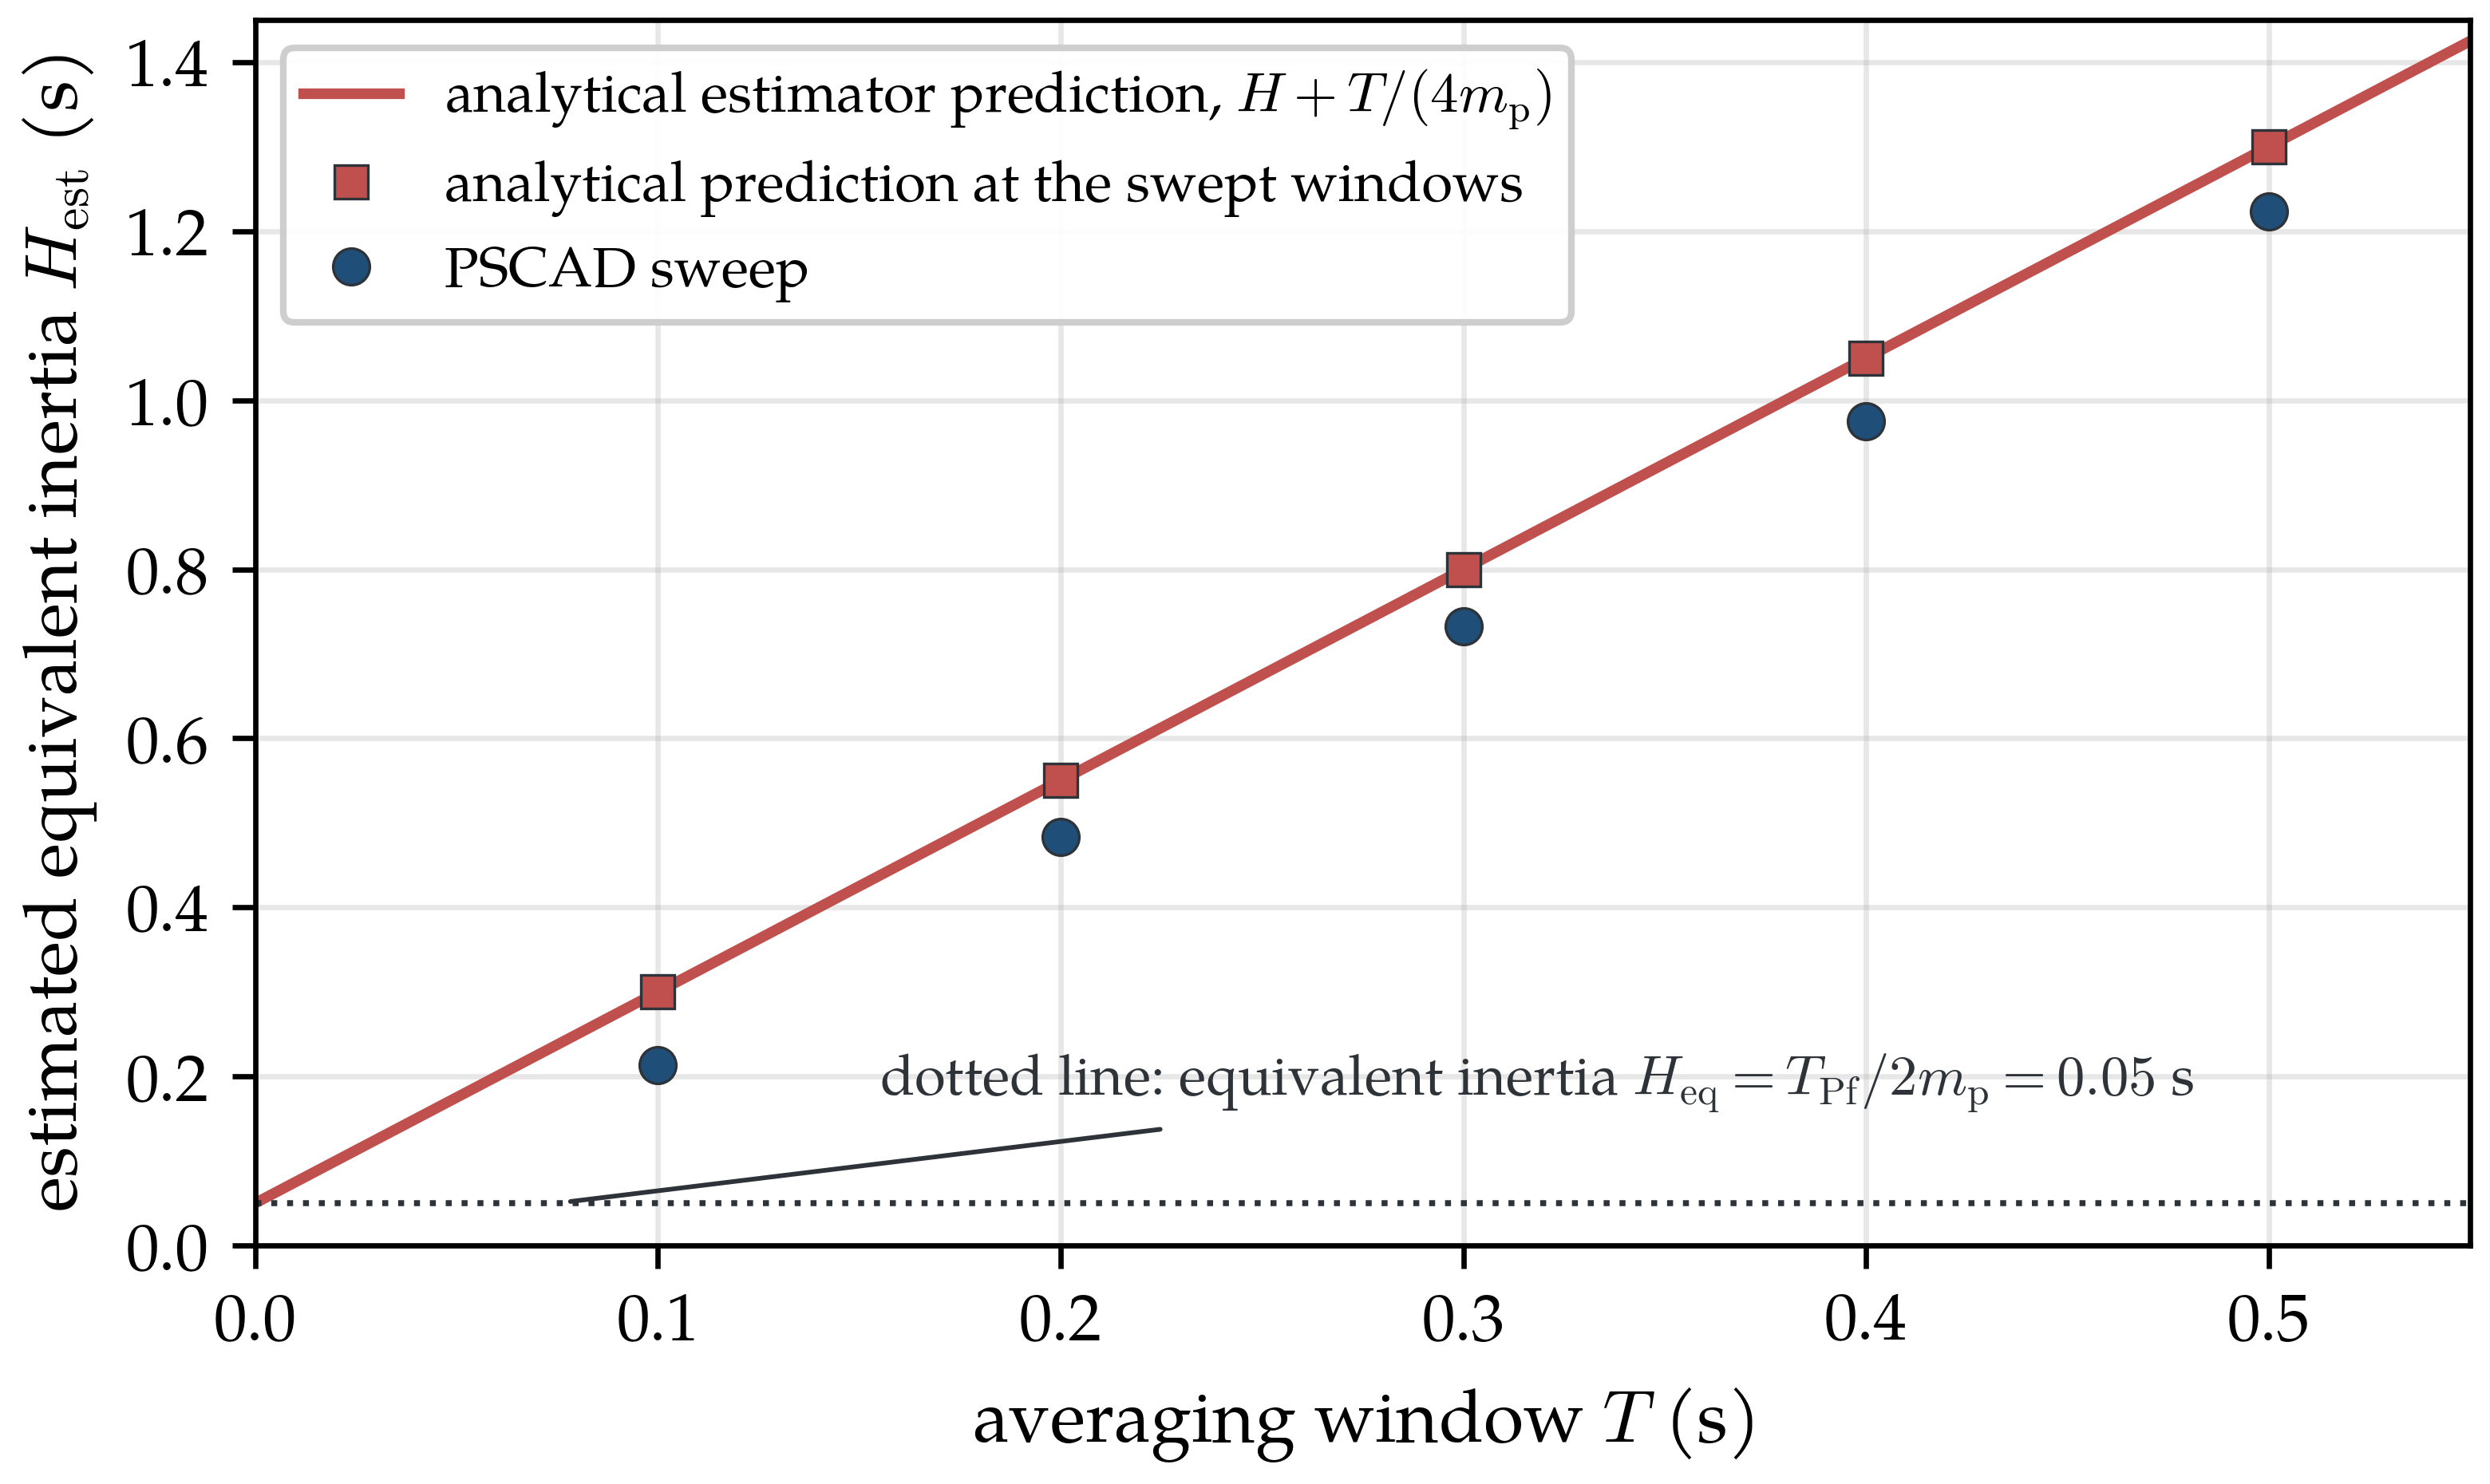
\includegraphics[width=0.8\textwidth]{hest_corrected}
\caption{Inertia estimate from Equation~\eqref{eq:hest} compared with the PSCAD integration-window sweep at $m_{\mathrm{p}}=0.1$: the line has intercept $T_{\mathrm{Pf}}/(2m_{\mathrm{p}})=0.05$~s, the equivalent inertia (dotted line), and slope $1/(4m_{\mathrm{p}})=2.5$. It predicts the inertia estimator output including damping, rather than an inertia estimate with damping removed.}
\label{fig:hestfit}
\end{figure}

At $m_{\mathrm{p}}=0.01$, the unsaturated expression predicts 13.0~s rather than 7.44~s. The inertia-test run was dispatched at $P=0$ with $P_{\max}=0.9$ per unit (Figure~\ref{fig:pscada1params}), so 0.9 per unit of active-power headroom was available; the reduced model requests 0.85 per unit by 0.5~s, within that headroom, and the active-power limit therefore does not explain the difference. The measured power reached 0.69 per unit at the end of the window. The remainder is the network between the imposed source frequency and the inverter's internal frequency. Figure~\ref{fig:hestscr} isolates it: the test was repeated at short-circuit ratios from 2 to 40 with the inverter's internal droop frequency recorded. Referred to the imposed ramp, the estimate rises from 6.3~s at a short-circuit ratio of 2 to 10.4~s at 40, because the internal frequency follows the imposed $-1$~Hz/s ramp only partially through the coupling reactance, at $-0.67$ to $-0.98$~Hz/s. Referred to the internal frequency, the frequency the controller actually responds to, the same records give 9.4 to 10.6~s, and 9.8 to 10.4~s over the 3 to 20 range previously reported. The grid-strength dependence of the published estimate is therefore the network's lag between the two frequencies, not a change in the controller; the residual between 10~s and the analytic 13.0~s is the controller's own dynamics inside the window.

Equation~\eqref{eq:hest} also suggests a damping correction. Since an underfrequency deviation is negative, removing the positive damping contribution requires
\begin{equation}
\Delta E_{\mathrm{in}}=\int_0^T\left[\Delta p(t)+D\frac{\Delta f(t)}{f_{\mathrm{n}}}\right]\,\mathrm{d}t.
\label{eq:subtract}
\end{equation}
Applying the same test normalization to this corrected energy yields $H$. The correction requires $\Delta p$ and $D$ on the same per-unit base and $\Delta f$ taken as the inverter's internal frequency, the one the droop responds to (Figure~\ref{fig:hestscr}). It recovers $H$ only where the reduced model holds: an active power limiter, the controller's own lag within the window, or the network's lag between the internal and imposed frequencies each leave a part of $\Delta p$ that is neither inertial nor $D\,\Delta f$.

Alternatively, the window dependence is
\begin{equation}
H_{\mathrm{est}}(T)=\underbrace{H}_{\text{intercept}}+
\underbrace{\frac{1}{4m_{\mathrm{p}}}}_{\text{slope}}T.
\label{eq:multiT}
\end{equation}
A window sweep could separate the intercept from the damping-related slope within this model. Figure~\ref{fig:hmech} illustrates the dependence on integration window and control configuration. A disabled virtual-inertia parameter does not necessarily eliminate the equivalent inertia created by filtered droop.

\begin{figure}[tbp]\centering
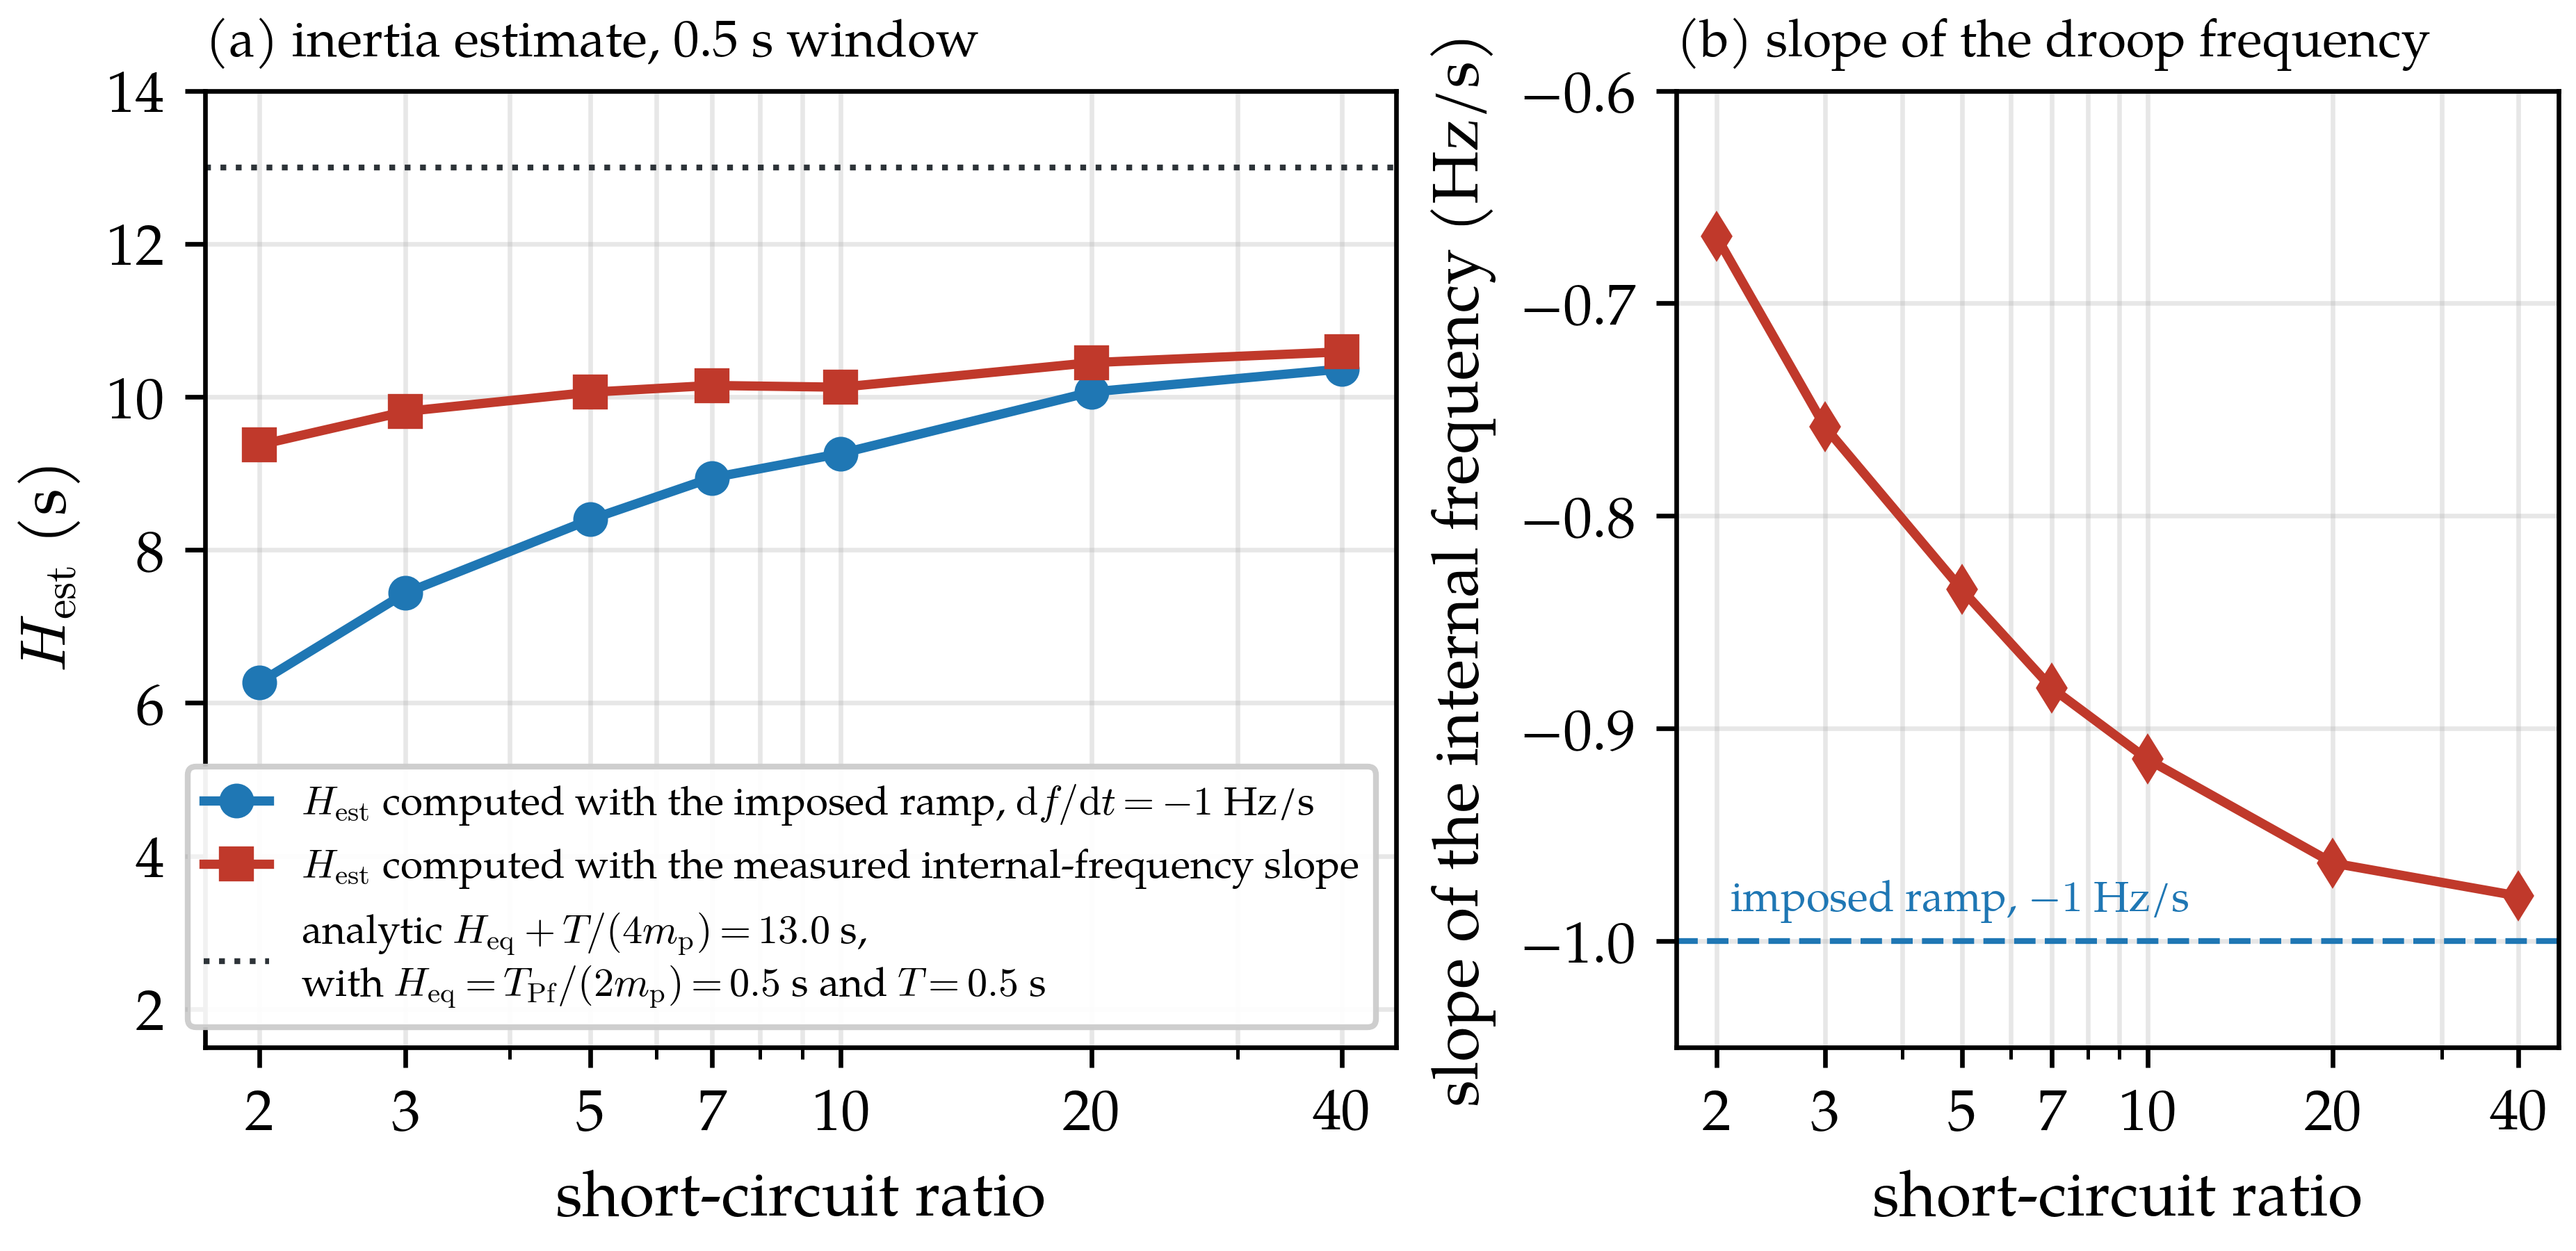
\includegraphics[width=0.95\textwidth]{narr_hest_vs_scr}
\caption{PMView inertia estimate of the droop-controlled inverter versus short-circuit ratio (Equation~\eqref{eq:scr}), 0.5~s window, dispatch $P=0$. (a)~The estimate referred to the imposed $-1$~Hz/s ramp, as in Equation~\eqref{eq:agsesr}, and referred to the inverter's internal droop frequency over the same window; the dotted line is the analytic $H_{\mathrm{eq}}+T/(4m_{\mathrm{p}})$. (b)~Least-squares slope of the internal droop frequency over the window, with the imposed $-1$~Hz/s ramp dashed; both are negative because the test is an under-frequency ramp.}
\label{fig:hestscr}
\end{figure}

\begin{figure}[tbp]\centering
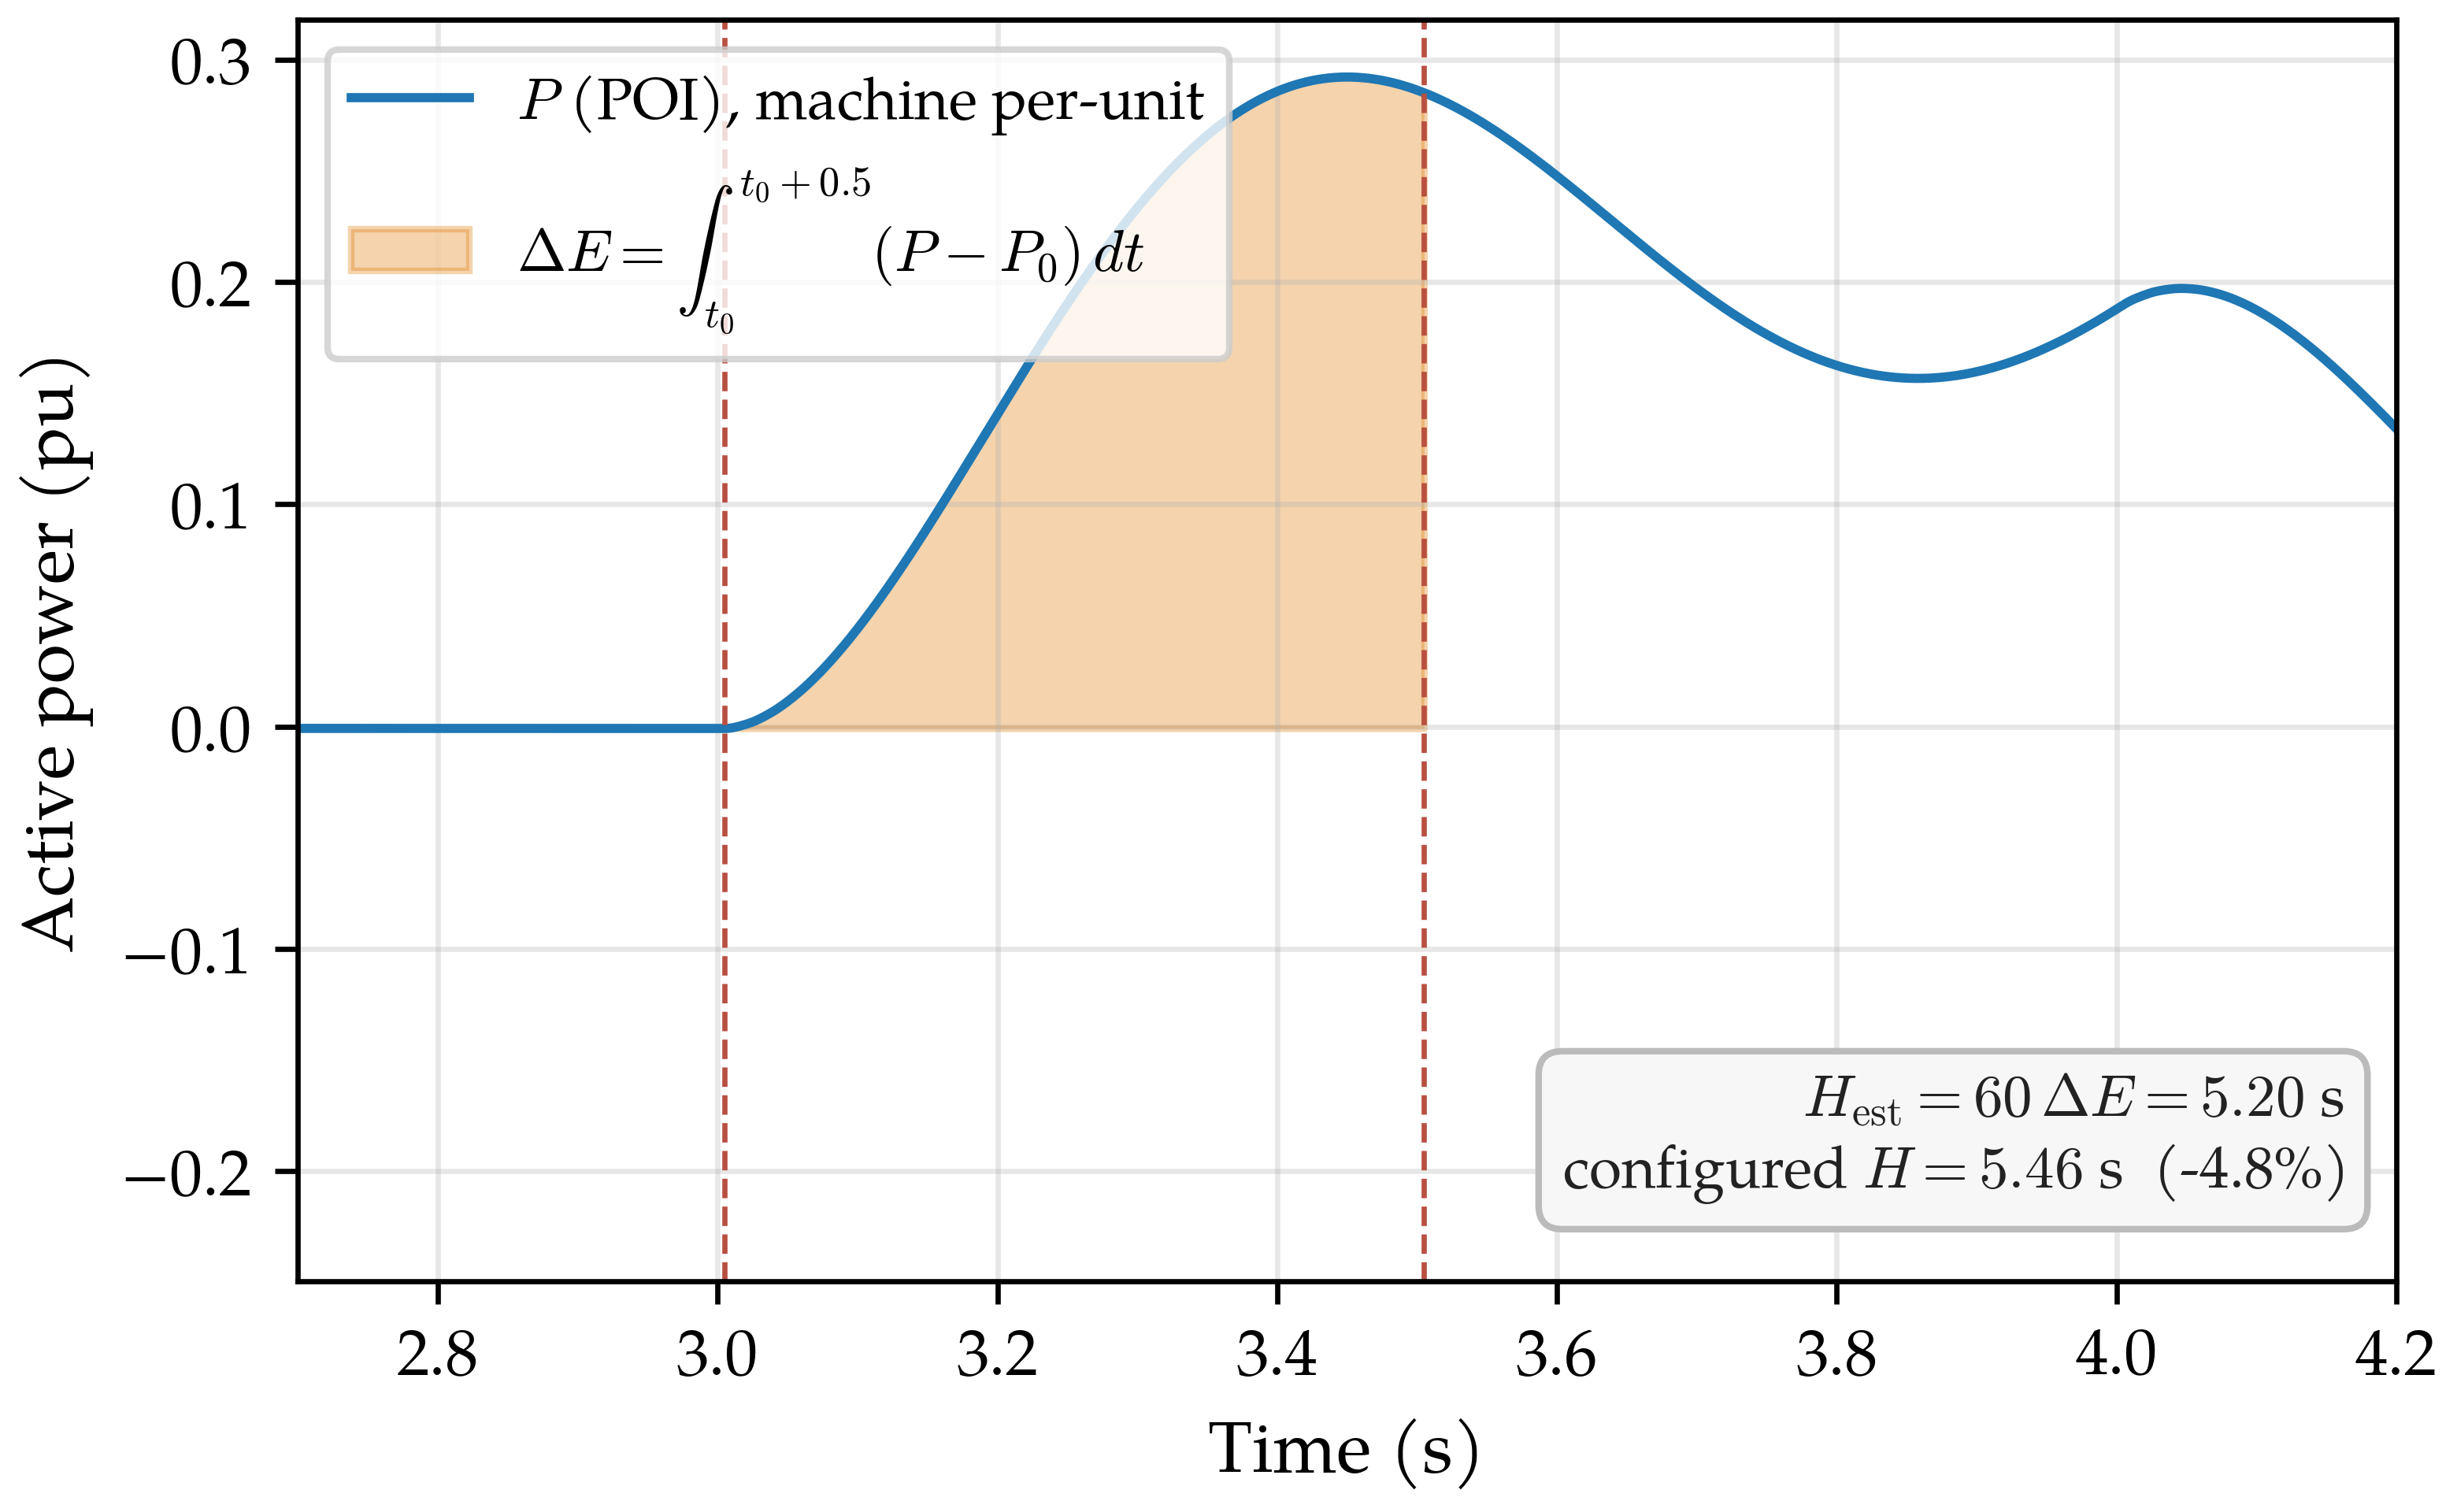
\includegraphics[width=0.8\textwidth]{fig9_inertia_sync}
\caption{PMView inertia estimation test for the synchronous machine: $H_{\mathrm{est}}=5.20$~s against the configured inertia $H=5.46$~s.}
\label{fig:hsync}
\end{figure}

\begin{figure}[tbp]\centering
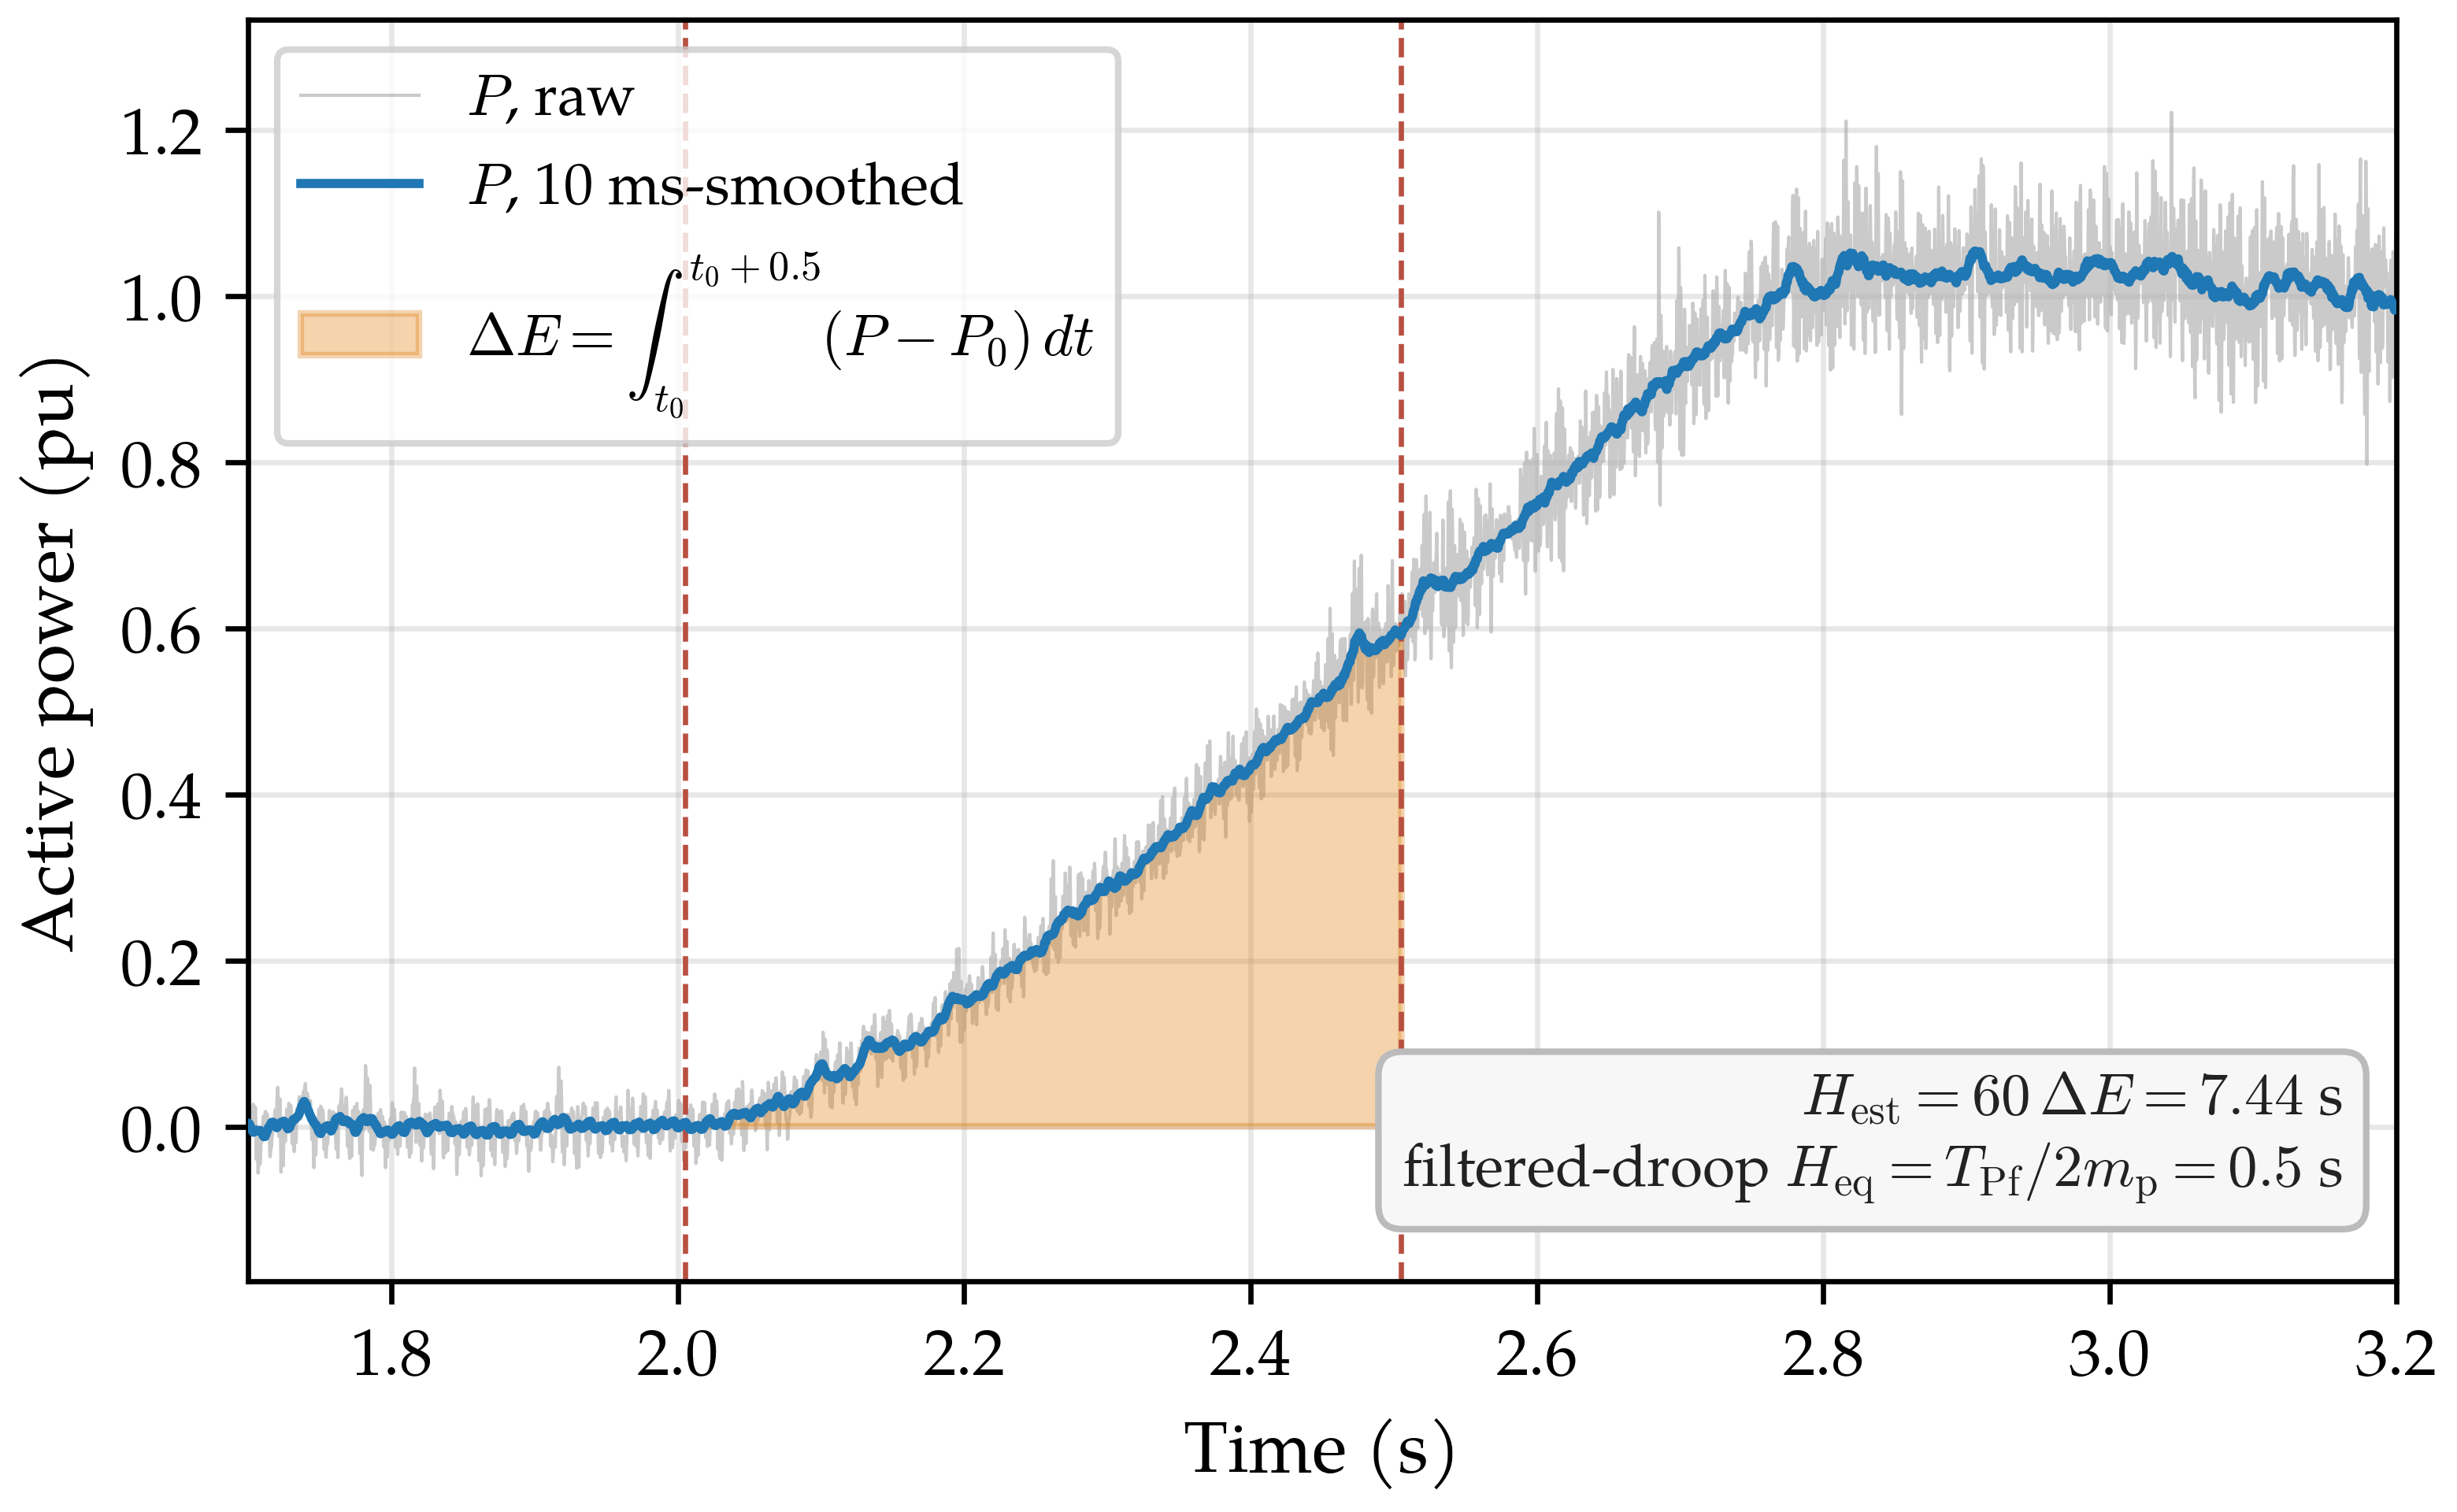
\includegraphics[width=0.8\textwidth]{fig10_inertia_gfm}
\caption{PMView inertia estimation test for the droop-controlled GFM inverter: $H_{\mathrm{est}}=7.44$~s, which includes the controller response and is distinct from the filtered-droop equivalent inertia.}
\label{fig:hgfm}
\end{figure}

\begin{figure}[tbp]\centering
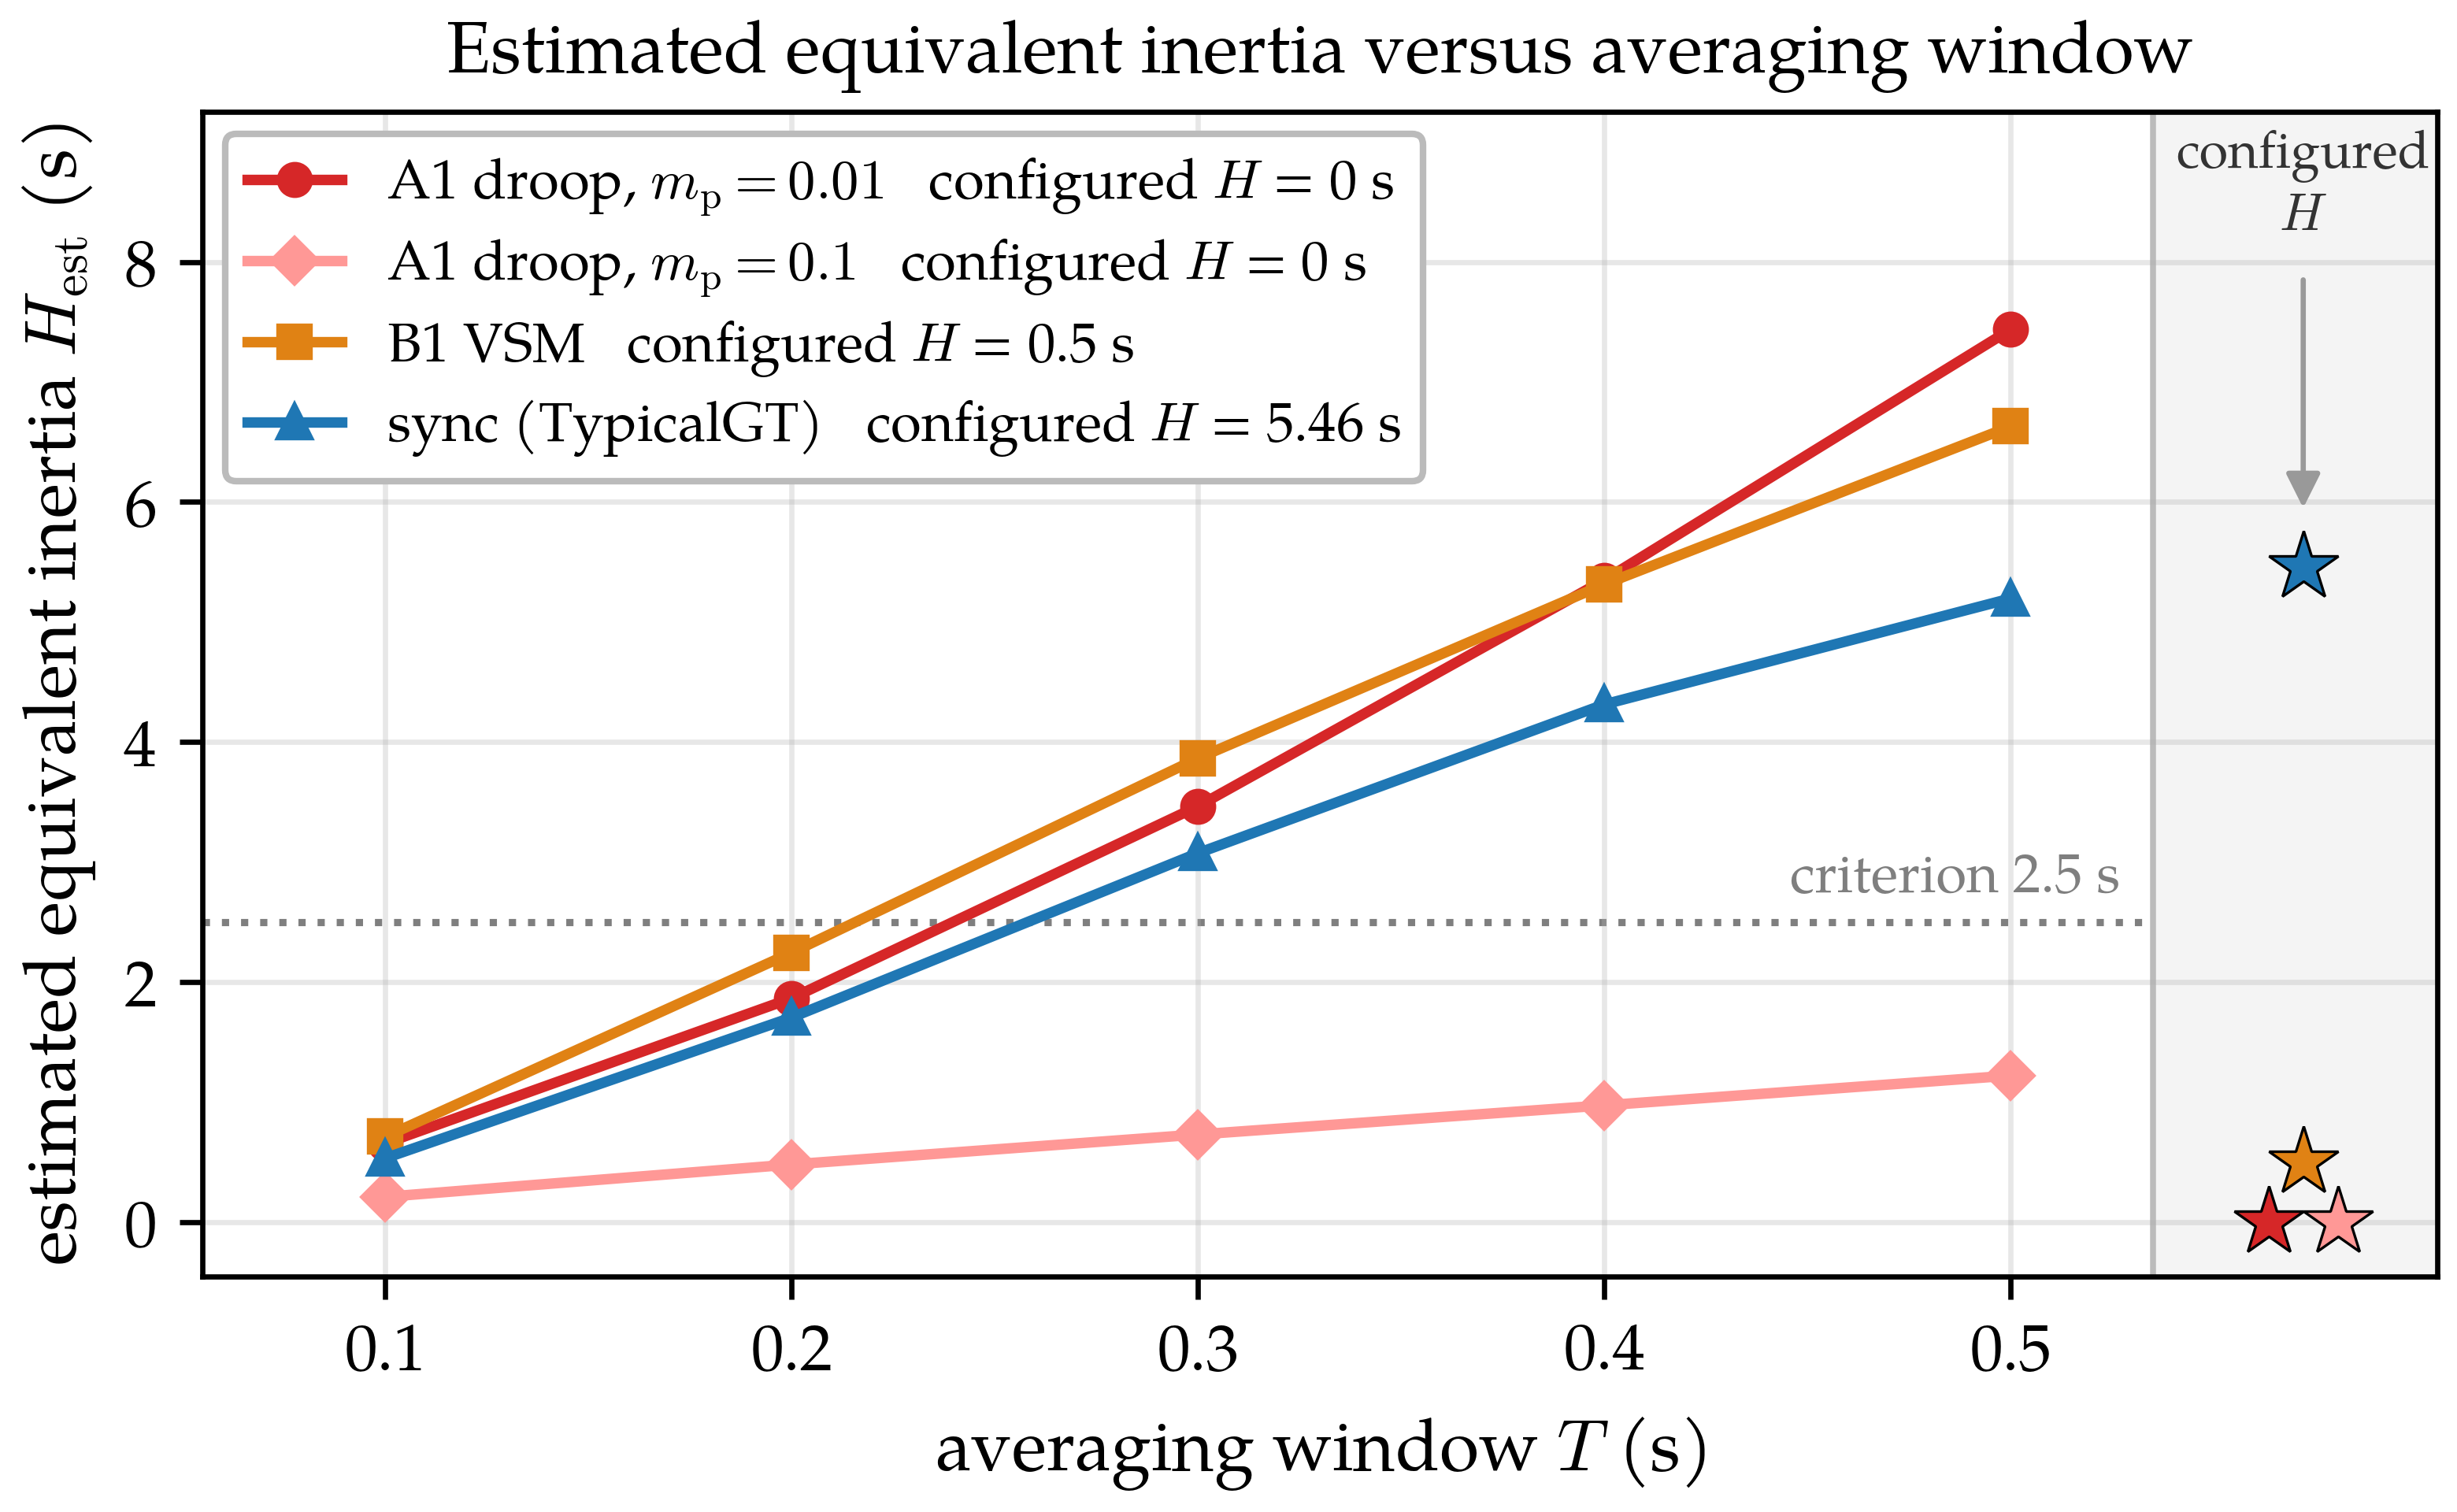
\includegraphics[width=0.8\textwidth]{fig11_inertia_mechanism_pair}
\caption{Estimated equivalent inertia versus integration-window length for the tested control configurations; the window dependence comes from the damping-related power response.}
\label{fig:hmech}
\end{figure}

\begin{figure}[tbp]\centering
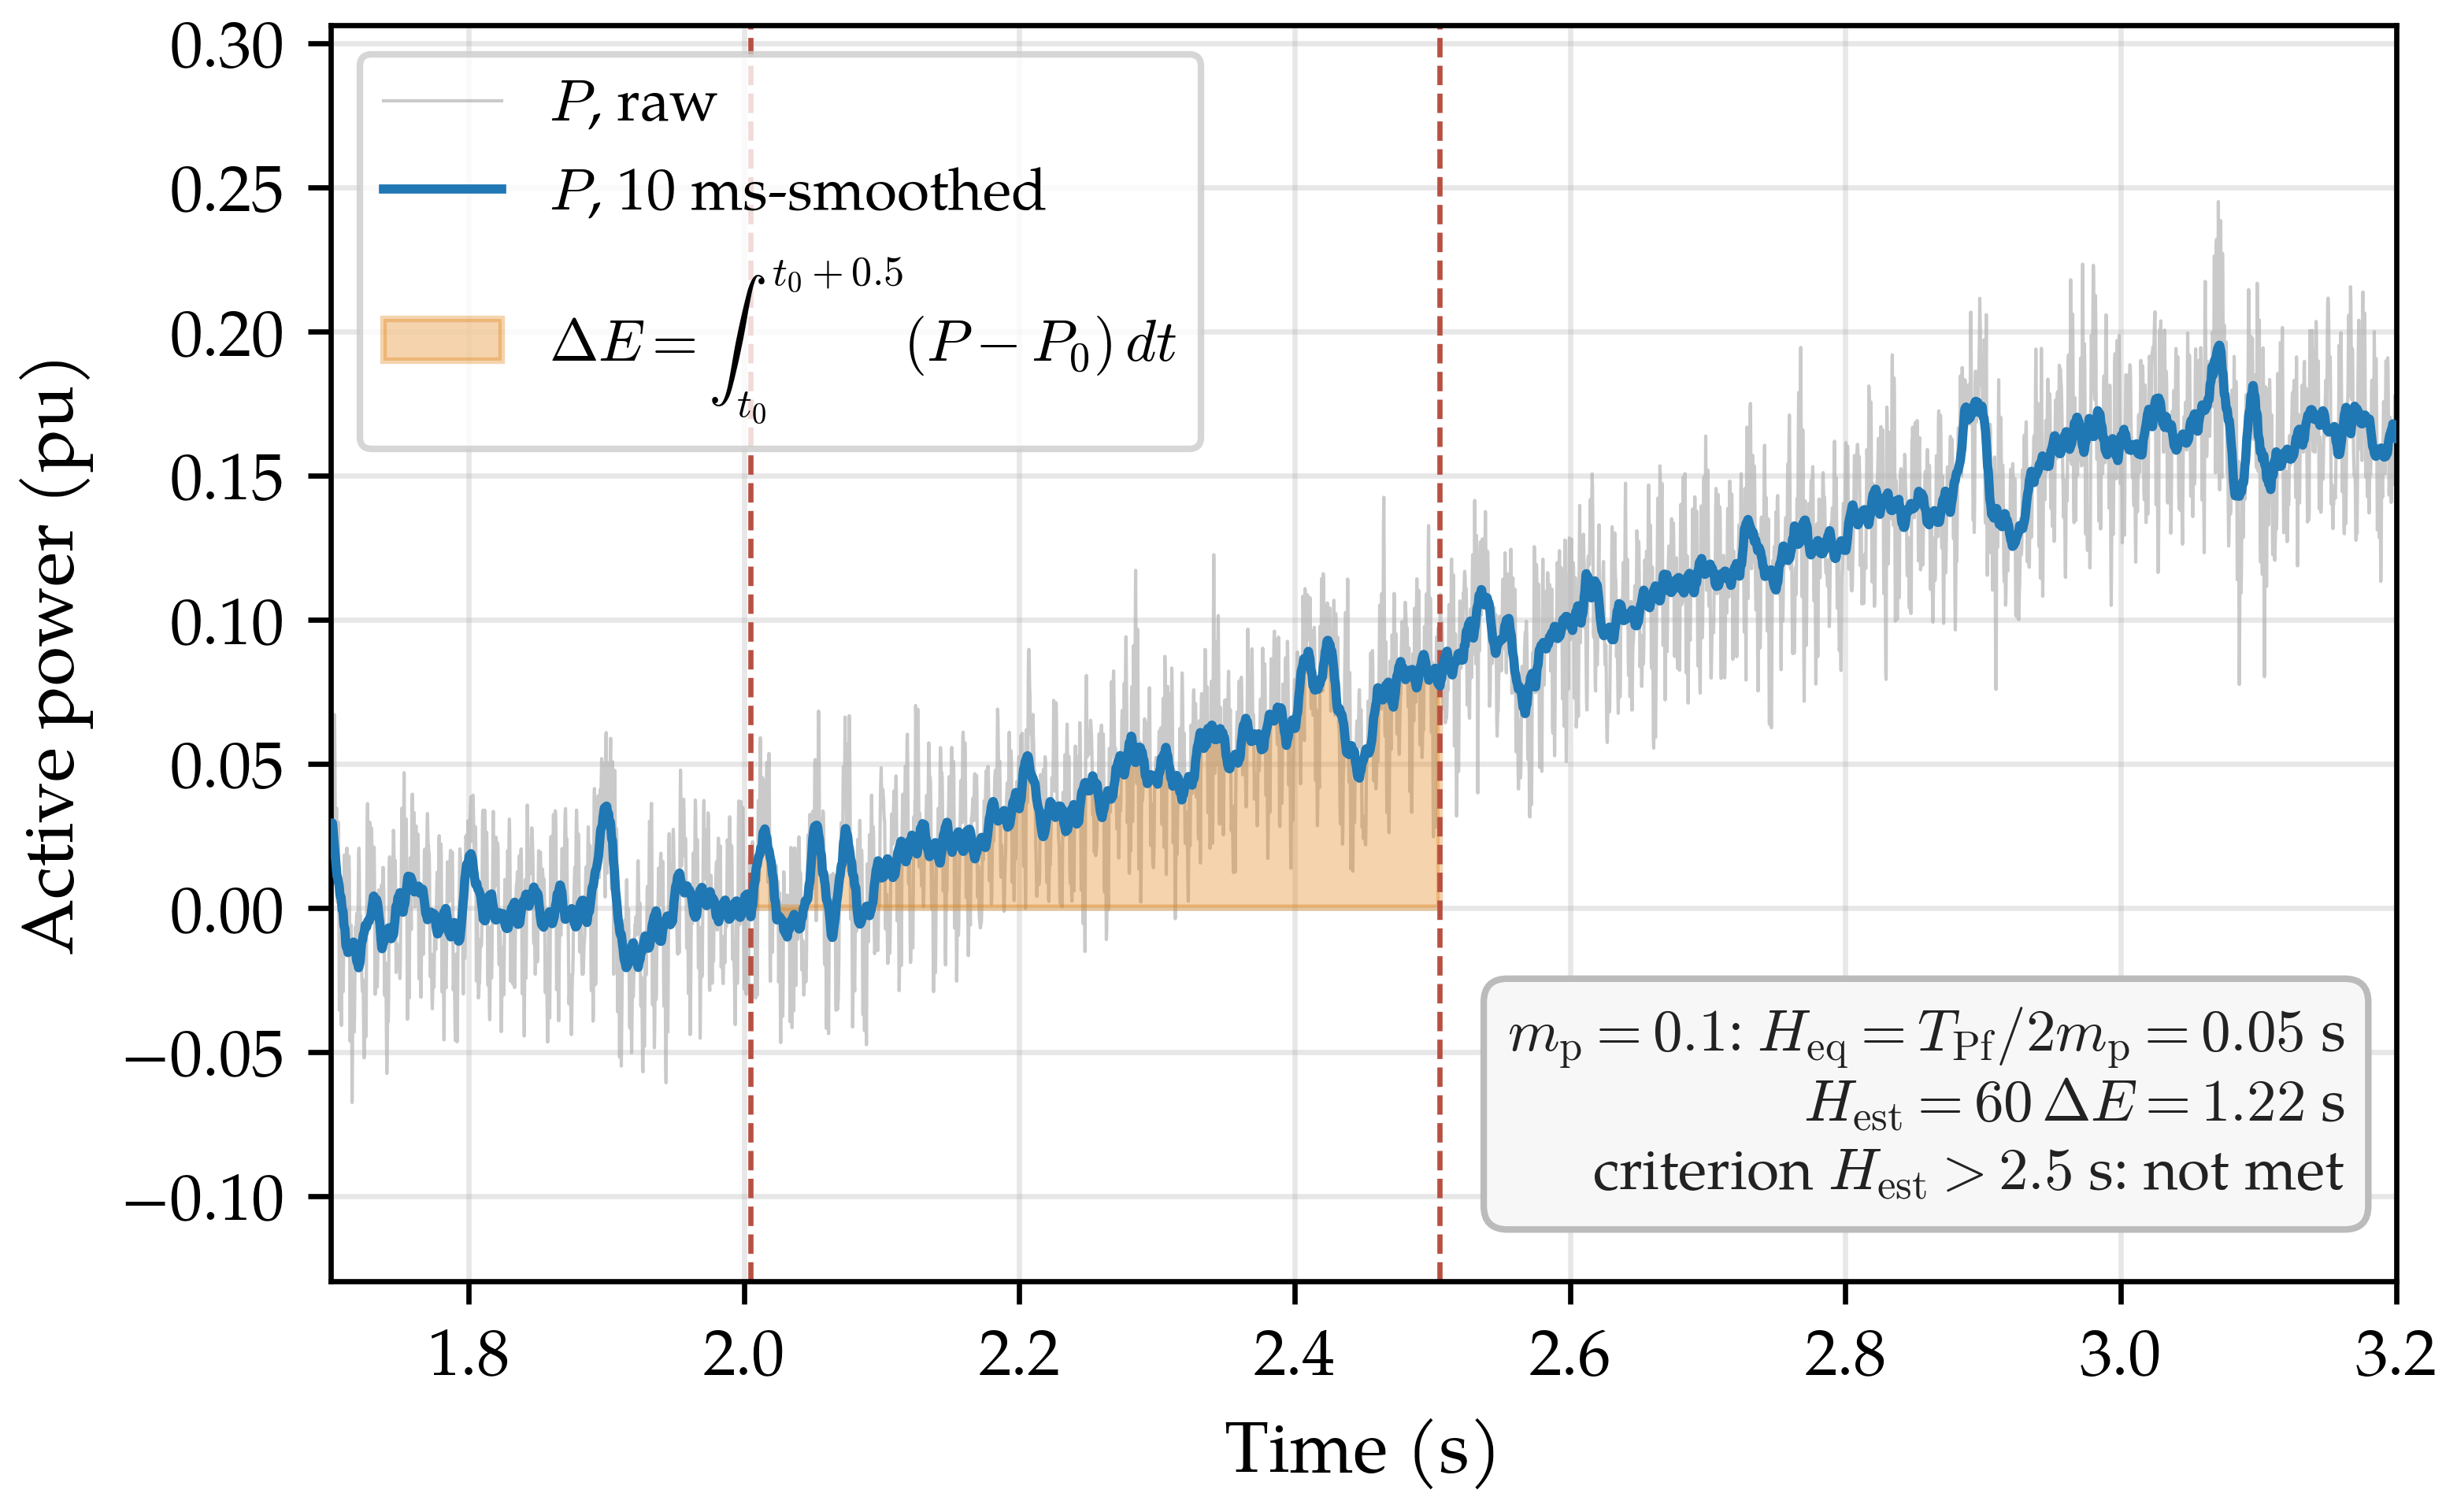
\includegraphics[width=0.8\textwidth]{narr_inertia_gfm_mp0p1}
\caption{GFM inertia estimation test at $m_{\mathrm{p}}=0.1$: $H_{\mathrm{est}}=1.22$~s; the weaker droop reduces both equivalent damping and filtered-droop equivalent inertia.}
\label{fig:mp01}
\end{figure}

\section{Next Steps and Conclusion}
\label{sec:outlook}
The first-year studies establish a platform for examining how inverter controls affect system-level stability. They also motivate analytical models that relate control parameters to fault-duration limits. The next phase will pair corresponding PSS/E and PSCAD studies while extending the preliminary energy analysis described below.

\subsection{Next Steps}
We will align network topology, operating points, device ratings, bases, applicable control settings, and disturbance definitions across the positive-sequence and EMT models. The purpose is to understand which dynamics each domain retains and how those differences affect engineering conclusions. We will not force identical trajectories from models that represent different phenomena. The adapted PSS/E network and its E-TRAN translation provide the common starting point.

The GFM studies show recovery across the tested replacement configurations, but they do not yet explain every control parameter's influence on stability. We therefore seek analytical estimates of the maximum tolerable fault duration for systems containing multiple GFM resources. Such estimates could help manufacturers and operators interpret the effects of droop, current limits, and voltage limits. The following preliminary exploration applies familiar machine-based methods before pursuing more detailed formulations.

\subsubsection{Preliminary Application of Classical Energy Methods}
\label{sec:energymethod}
Classical energy-function methods offer a familiar bridge from synchronous-machine stability analysis to GFM research \cite{sauer1998,pai1989,athay1979,bergen1981,chiang1988}. These methods compare an energy-like measure of the post-fault state with an energy boundary associated with unstable equilibria. They can provide sufficient stability conditions for the assumed model without following every subsequent swing. Applying them to GFM systems requires attention to the assumptions behind the power-angle relationship and damping representation.

For the post-fault system with center-of-inertia states $(\theta,\tilde\omega)$, the transient energy function is the first integral of the swing equations \cite{sauer1998},
\begin{equation}
V(\theta,\tilde\omega)=\frac12\sum_{i}M_i\tilde\omega_i^2-\sum_{i}\int_{\theta_i^{\mathrm{s}}}^{\theta_i}f_i(\theta)\,\mathrm{d}\theta_i=V_{\mathrm{KE}}+V_{\mathrm{PE}},
\label{eq:tef}
\end{equation}
where $f_i$ is the accelerating power of device $i$ in the center-of-inertia frame and $\theta^{\mathrm{s}}$ is the post-fault stable equilibrium. Written out for $n$ devices represented as constant internal voltages $E_i$ behind their coupling reactances, with the network reduced to those internal nodes \cite{sauer1998},
\begin{equation}
f_i(\theta)=P_{\mathrm{m},i}-P_{\mathrm{e},i}(\theta)-\frac{M_i}{M_{\mathrm{T}}}P_{\mathrm{COI}}(\theta),\qquad
P_{\mathrm{e},i}(\theta)=E_i\sum_{j=1}^{n}E_j\left[G_{ij}\cos(\theta_i-\theta_j)+B_{ij}\sin(\theta_i-\theta_j)\right],
\label{eq:fi}
\end{equation}
with $P_{\mathrm{COI}}=\sum_i(P_{\mathrm{m},i}-P_{\mathrm{e},i})$ and $M_{\mathrm{T}}=\sum_i M_i$. Here $P_{\mathrm{m},i}$ is the mechanical power of a machine or the power reference $p^{*}$ of an inverter, and $G_{ij}$ and $B_{ij}$ are the conductance and susceptance of the reduced network between internal nodes $i$ and $j$; in the 39-bus cases the electrical power is taken from the constant-power network solution instead of a reduced admittance matrix, with the same dependence on the internal voltages and the coupling reactances. So $f_i$, and with it the potential energy $V_{\mathrm{PE}}$ and the shape of the surfaces in Figures~\ref{fig:esbelow} and~\ref{fig:esat}, contain the dispatch, the internal voltages, and the network admittances only. 

The inertia coefficients enter the kinetic term and the center-of-inertia weighting $M_i/M_{\mathrm{T}}$, and the damping coefficients $D_i$ do not appear in $V$ at all. Damping acts only on how $V$ changes along a trajectory. Without damping, $\mathrm{d}V/\mathrm{d}t=0$ along post-fault trajectories, so a state with $V<V_{\mathrm{cr}}$, the potential energy at the unstable equilibrium that bounds the basin, cannot reach that boundary: $V$ is a Lyapunov function, that is, a function that is positive about the equilibrium and non-increasing along the system's trajectories \cite{khalil2002}, and $V<V_{\mathrm{cr}}$ is a sufficient stability condition. 

The machine estimates below use $D=0$. For the droop inverters the damping $D_i=1/m_{\mathrm{p}}$ is retained; because every unit shares the same power-filter time constant, the ratio $D_i/M_i=1/T_{\mathrm{Pf}}$ is the same on every unit, the center-of-inertia transform remains exact, and $\mathrm{d}V/\mathrm{d}t=-\sum_i D_i\tilde\omega_i^2\le 0$, so the same bound holds with the damping in place. For the single-machine model, $V_{\mathrm{cr}}=V_{\mathrm{PE}}(\delta_{\mathrm{u}})$, and the condition $V\le V_{\mathrm{cr}}$ at clearing is the equal-area criterion. 

The critical clearing time follows in three steps: compute $\theta^{\mathrm{s}}$; obtain $V_{\mathrm{cr}}$ from the unstable equilibrium or, in the potential-energy-boundary-surface (PEBS) screen, from the maximum of $V_{\mathrm{PE}}$ along the sustained-fault trajectory; integrate the fault-on equations from the pre-fault equilibrium and record the time at which $V$ reaches $V_{\mathrm{cr}}$. In this report each device is modeled as a constant voltage behind reactance, $E'$ behind $X'_{\mathrm{d}}$ for the machines and the reduced droop model of Equation~\eqref{eq:gfmswing} for the inverters, with coefficients converted to the system base. The 39-bus network is retained with the model's constant-power loads, the fault is the bolted bus-14 fault with the network intact, and $V_{\mathrm{PE}}$ is evaluated as the path integral in Equation~\eqref{eq:tef} along the computed trajectory. The quoted estimates are the bisection limits of the integrated reduced model, with stability defined by bounded post-clearing angles; the PEBS screen gives 0.228~s for the ten-machine case.

For the constant-voltage, lossless single-machine model in Equation~\eqref{eq:swingeq}, the stable and unstable equilibria satisfy
\begin{equation}
\delta_{\mathrm{s}}=\arcsin(p_{\mathrm{m}}/p_{\mathrm{max}}),\qquad
\delta_{\mathrm{u}}=\pi-\delta_{\mathrm{s}},
\label{eq:equilibria}
\end{equation}
for the positive-power operating branch with $0<p_{\mathrm{m}}<p_{\mathrm{max}}$. The unstable equilibrium helps define the energy boundary, but its angle alone is not a complete transient-stability criterion because speed also contributes. An energy estimate combines the fault-on trajectory and the post-fault boundary to estimate critical clearing time. That time is the maximum fault duration satisfying the selected post-fault stability criterion.

We compare analytical estimates with brackets $(a,b]$ formed by a successful simulation at duration $a$ and an unsuccessful simulation at $b$. The angle-based comparisons distinguish return toward the original equilibrium from a phase slip into a neighboring angle region. A phase slip does not necessarily imply sustained loss of synchronism, and an unwrapped angle near $360^\circ$ alone does not show whether the system later resynchronizes. These distinctions matter when interpreting critical clearing time as a practical ride-through limit.

Figure~\ref{fig:efcct} summarizes the preliminary comparisons. The machine estimates hold the mechanical power constant and omit the exciter, governor, and stabilizer; the single-machine case is lossless with zero electrical power during the bolted fault. The GFM estimates use the swing-form droop model of Equation~\eqref{eq:heqdeq} with $H_{\mathrm{eq}}=0.5$~s and $D=1/m_{\mathrm{p}}=100$, a constant internal voltage behind the filter and transformer reactance, and no current or voltage limit. For the single-machine case, the 0.474~s estimate is below the demonstrated stable duration of 0.622~s. For the 39-bus machine case, the 0.248~s estimate lies inside the $(0.237,0.250]$~s simulation bracket. An estimate inside a bracket is consistent with its resolution but is not, by itself, demonstrably conservative.

\begin{figure}[tbp]\centering
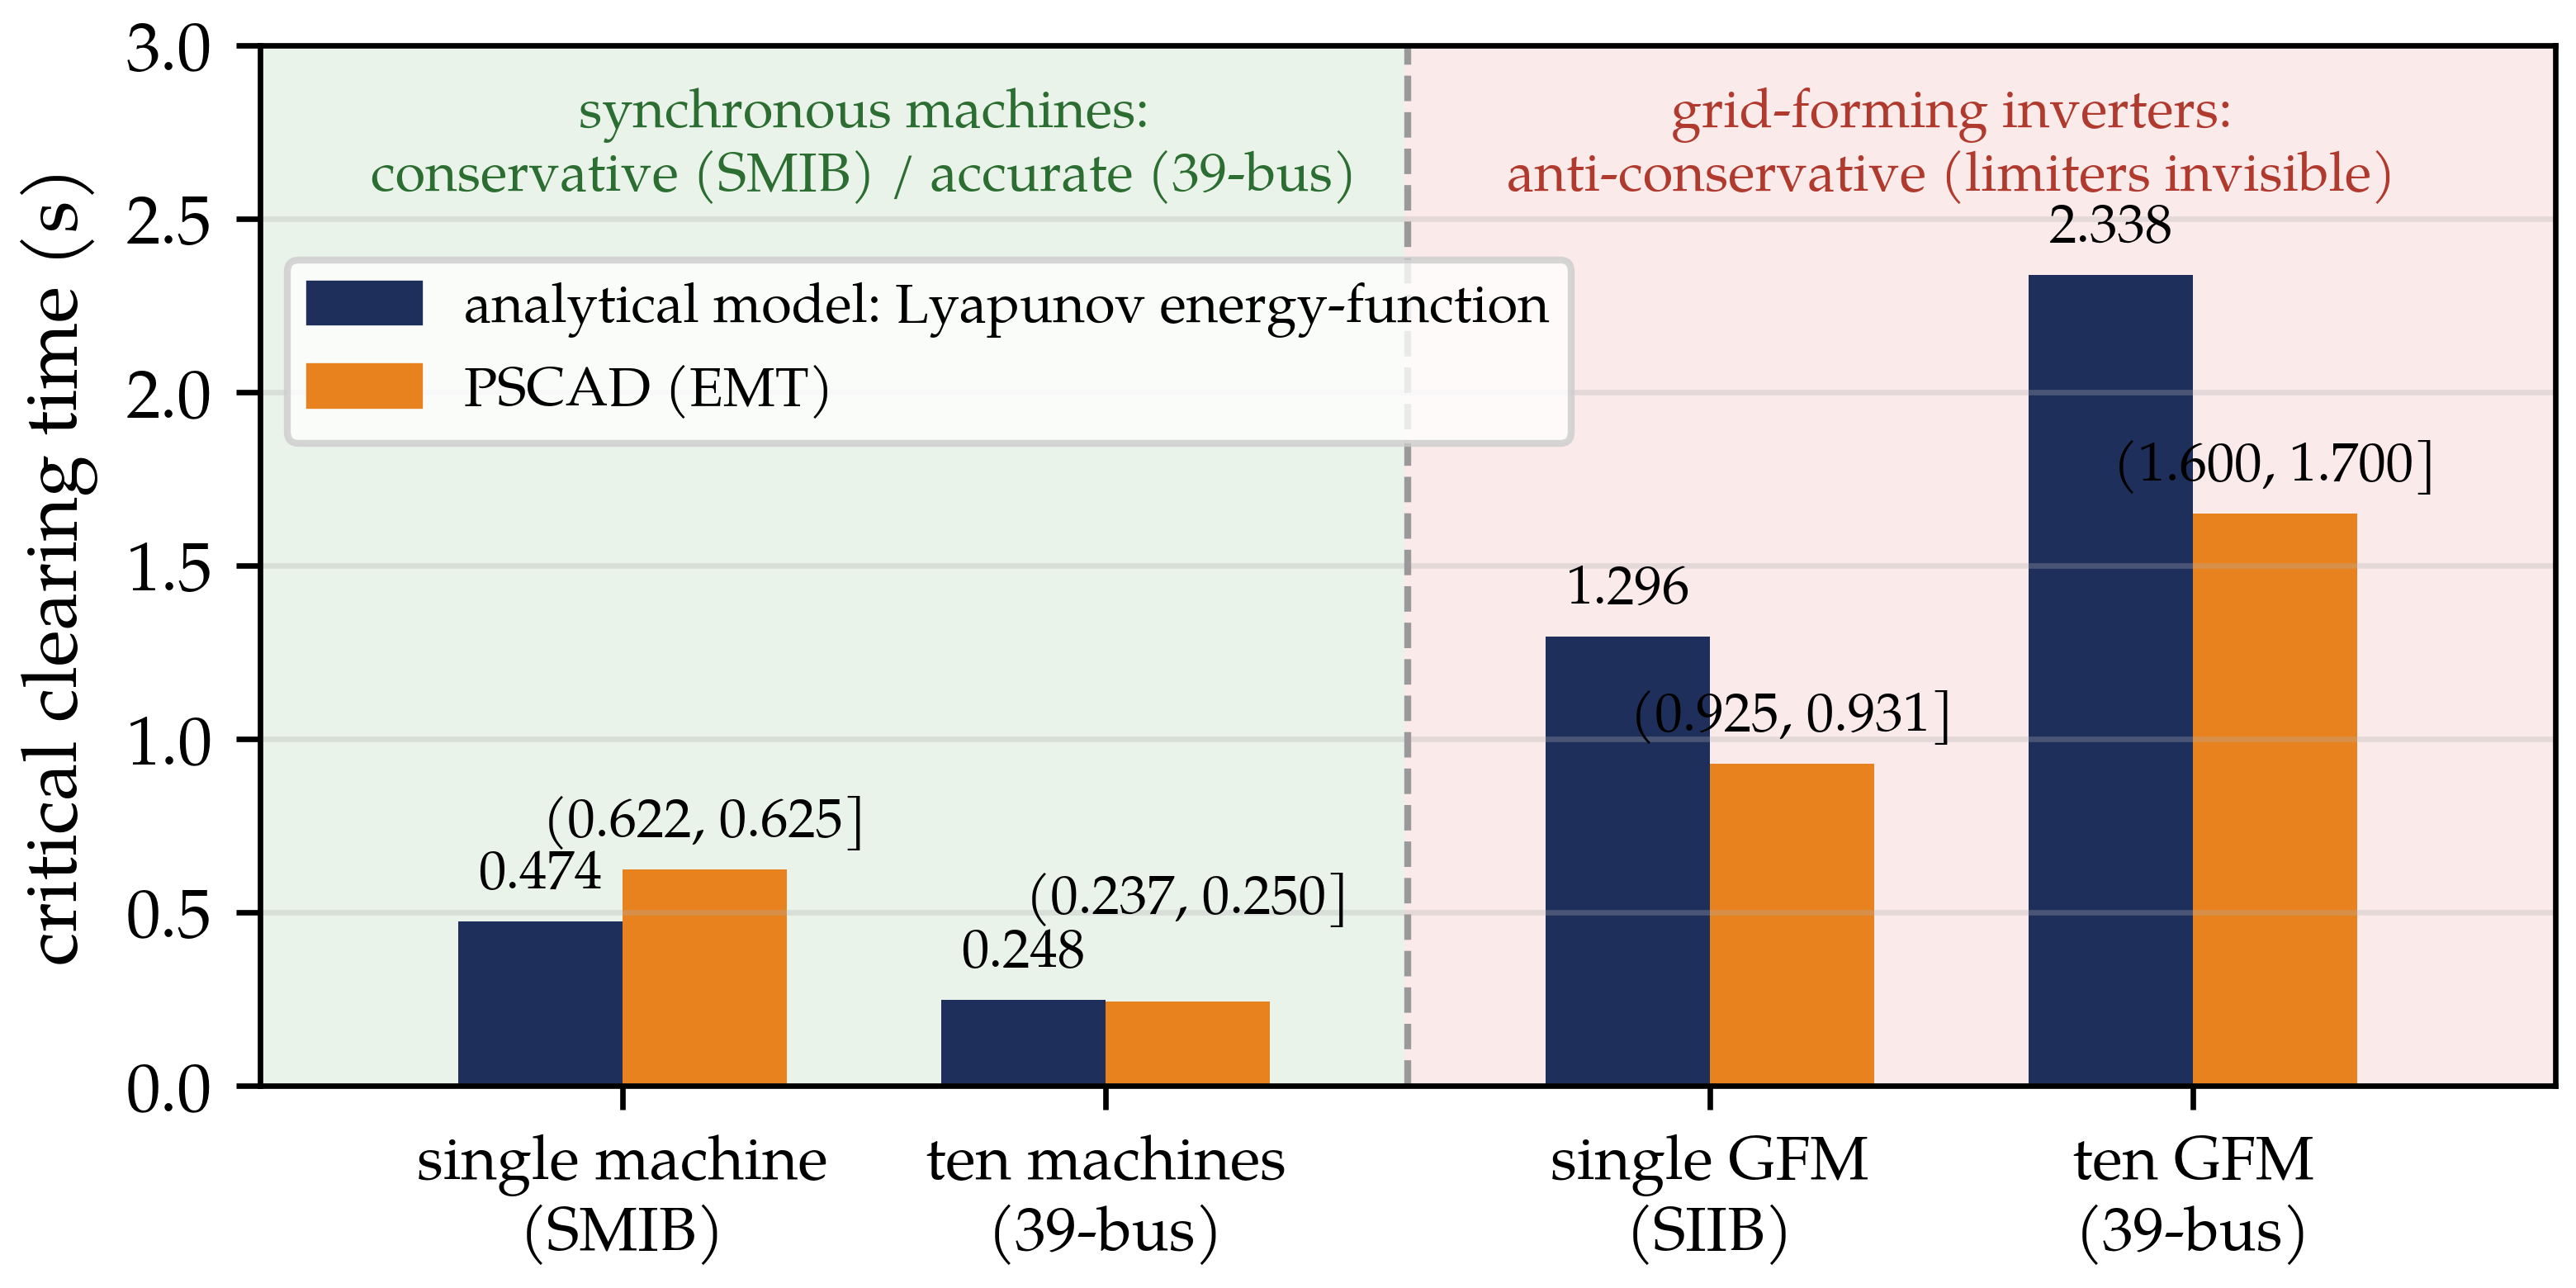
\includegraphics[width=0.8\textwidth]{ef_cct_machines_vs_gfm}
\caption{Energy-method critical clearing times (navy) compared with PSCAD EMT brackets (orange), each bracket running from a successful to an unsuccessful clearing duration. The estimates are single values from the reduced models of Section~\ref{sec:energymethod}: the machine model is the undamped classical one, and the inverter model includes the droop damping $D=1/m_{\mathrm{p}}$ but no current limiter, which is why its estimates exceed their brackets (Section~\ref{sec:gfmgap}).}
\label{fig:efcct}
\end{figure}

Following the center-of-inertia (COI) formulation in Sauer and Pai, Chapter~9, Section~9.5, Equation~(9.19) \cite{sauer1998}, define
\begin{equation}
\delta_{\mathrm{COI}}=\frac{\sum_{i=1}^{n}M_i\delta_i}{\sum_{i=1}^{n}M_i},
\qquad \theta_i=\delta_i-\delta_{\mathrm{COI}},
\qquad \tilde\theta_i=\theta_i-\theta_i^{\mathrm{s}}.
\label{eq:energycoi}
\end{equation}
Here $M_i$ is the inertia coefficient in the reduced angular-acceleration equation, expressed on a common system base, and $\theta_i^{\mathrm{s}}$ is the reference stable-equilibrium angle. For a synchronous machine, $\delta_i$ is the electrical rotor angle. For a GFM inverter, it is the controller-generated electrical angle; the analogous COI uses the reduced model's equivalent inertia coefficients, not physical rotor inertia. The plotted coordinates $\tilde\theta_{31}$ and $\tilde\theta_{32}$ are therefore equilibrium-shifted angles of the resources at buses~31 and~32 relative to the fleet's COI, not pairwise inter-machine angles. The reference equilibrium appears at the origin.

Figure~\ref{fig:esbelow} shows the machine and GFM trajectories at their last stable clearing durations, 0.237~s and 1.6~s, respectively. The two-dimensional (2D) contours display analytical potential energy over these COI coordinates. Both responses remain near the reference equilibrium after clearing, although the marked model and EMT endpoints need not coincide. The white boundary is the reduced model's critical-energy boundary estimate; a two-angle view does not certify a basin boundary for the complete EMT system, whose state also includes speeds and other control variables.

\begin{figure}[tbp]\centering
\energycontour{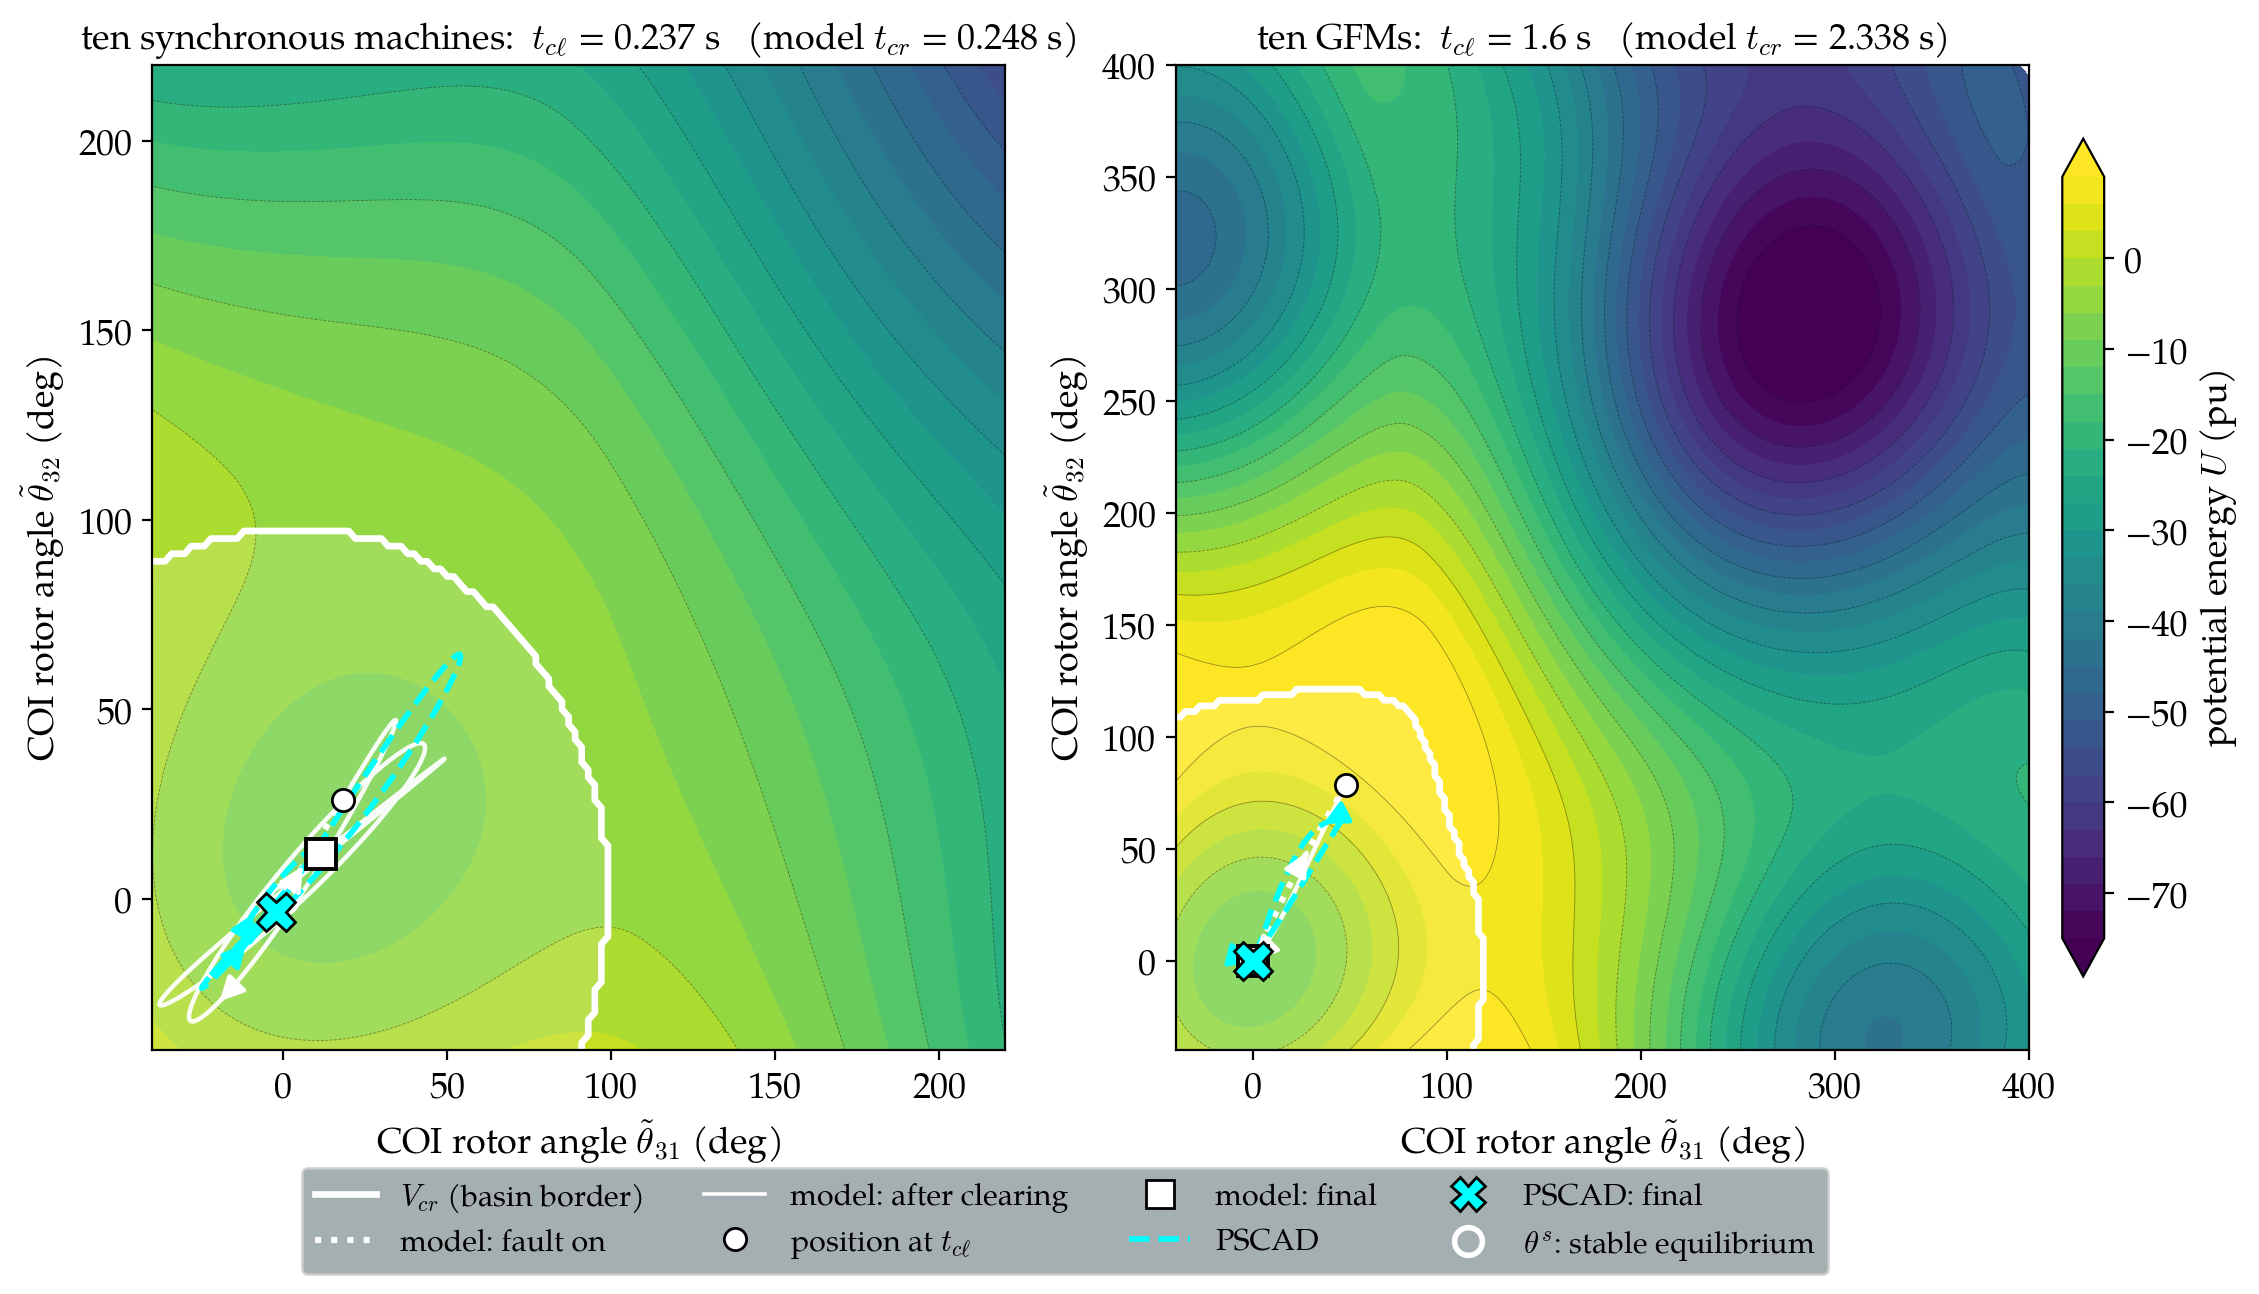
\includegraphics[width=\linewidth]{prism-uploads/below_cct_surface_meeting.png}}{0.237}{1.600}
\caption{Potential-energy contours in equilibrium-shifted COI coordinates for the 39-bus system at the last stable clearing durations: (a)~ten synchronous machines, 0.237~s, and (b)~ten GFM inverters, 1.600~s. White dotted and thin solid curves show the model's fault-on and post-clearing paths, cyan dashed curves the PSCAD EMT trajectories, and the thick white curve the model boundary estimate. Circles mark clearing, squares model endpoints, and cyan crosses EMT endpoints.}
\label{fig:esbelow}
\end{figure}

\subsubsection{Limits of the Present Energy Construction}
\label{sec:gfmgap}
The same classical construction overestimates the clearing margin for the tested GFM cases. In the 39-bus comparison, it predicts approximately 2.34~s against an EMT bracket of $(1.6,1.7]$~s. In the single-inverter infinite-bus comparison, it predicts 1.296~s against $(0.925,0.931]$~s. These differences are larger than in the corresponding machine comparisons and motivate a more detailed treatment of inverter controls.

Figure~\ref{fig:esat} compares clearing near each analytical critical clearing time using complementary 2D and three-dimensional (3D) views of the same cases. The contours make the trajectories and endpoints easier to compare, while the 3D surfaces expose the potential-energy ridge and neighboring well. At 0.2455~s, the machine EMT trajectory returns near the reference equilibrium. At 2.315~s, the GFM EMT trajectory crosses the ridge and ends near $(\tilde\theta_{31},\tilde\theta_{32})=(290^\circ,290^\circ)$ in the supplied COI-coordinate view, while the analytical trajectory returns toward the origin. The trajectories disagree on return to the original equilibrium, which is a more specific observation than a claim that the inverter never resynchronizes.

The larger amplitude and curvature of the GFM surface follow from the coupling reactances, not from the inertia or damping coefficients: neither appears in $f_i$ of Equation~\eqref{eq:fi}, so neither enters the potential energy of Equation~\eqref{eq:tef}. Each inverter is represented as $E$ behind $X_{\mathrm{L}}=0.15$ per unit on its base $S_{\mathrm{inv,base}}=P_{\mathrm{G}}/0.6$, the example value of the model specification \cite{du2023a1}, whereas each machine is $E'$ behind $X'_{\mathrm{d}}=0.26$ per unit on its rating; on the system base the inverter internal nodes are coupled through 2.8--2.9 times less reactance at nine of the ten buses, and the curvature of the surface at the equilibrium is 1.9 times the machine value. Recomputing the inverter surface with the machines' system-base reactances brings that curvature to within 25\% of the machine value.

\begin{figure}[p]\centering
\energycontour{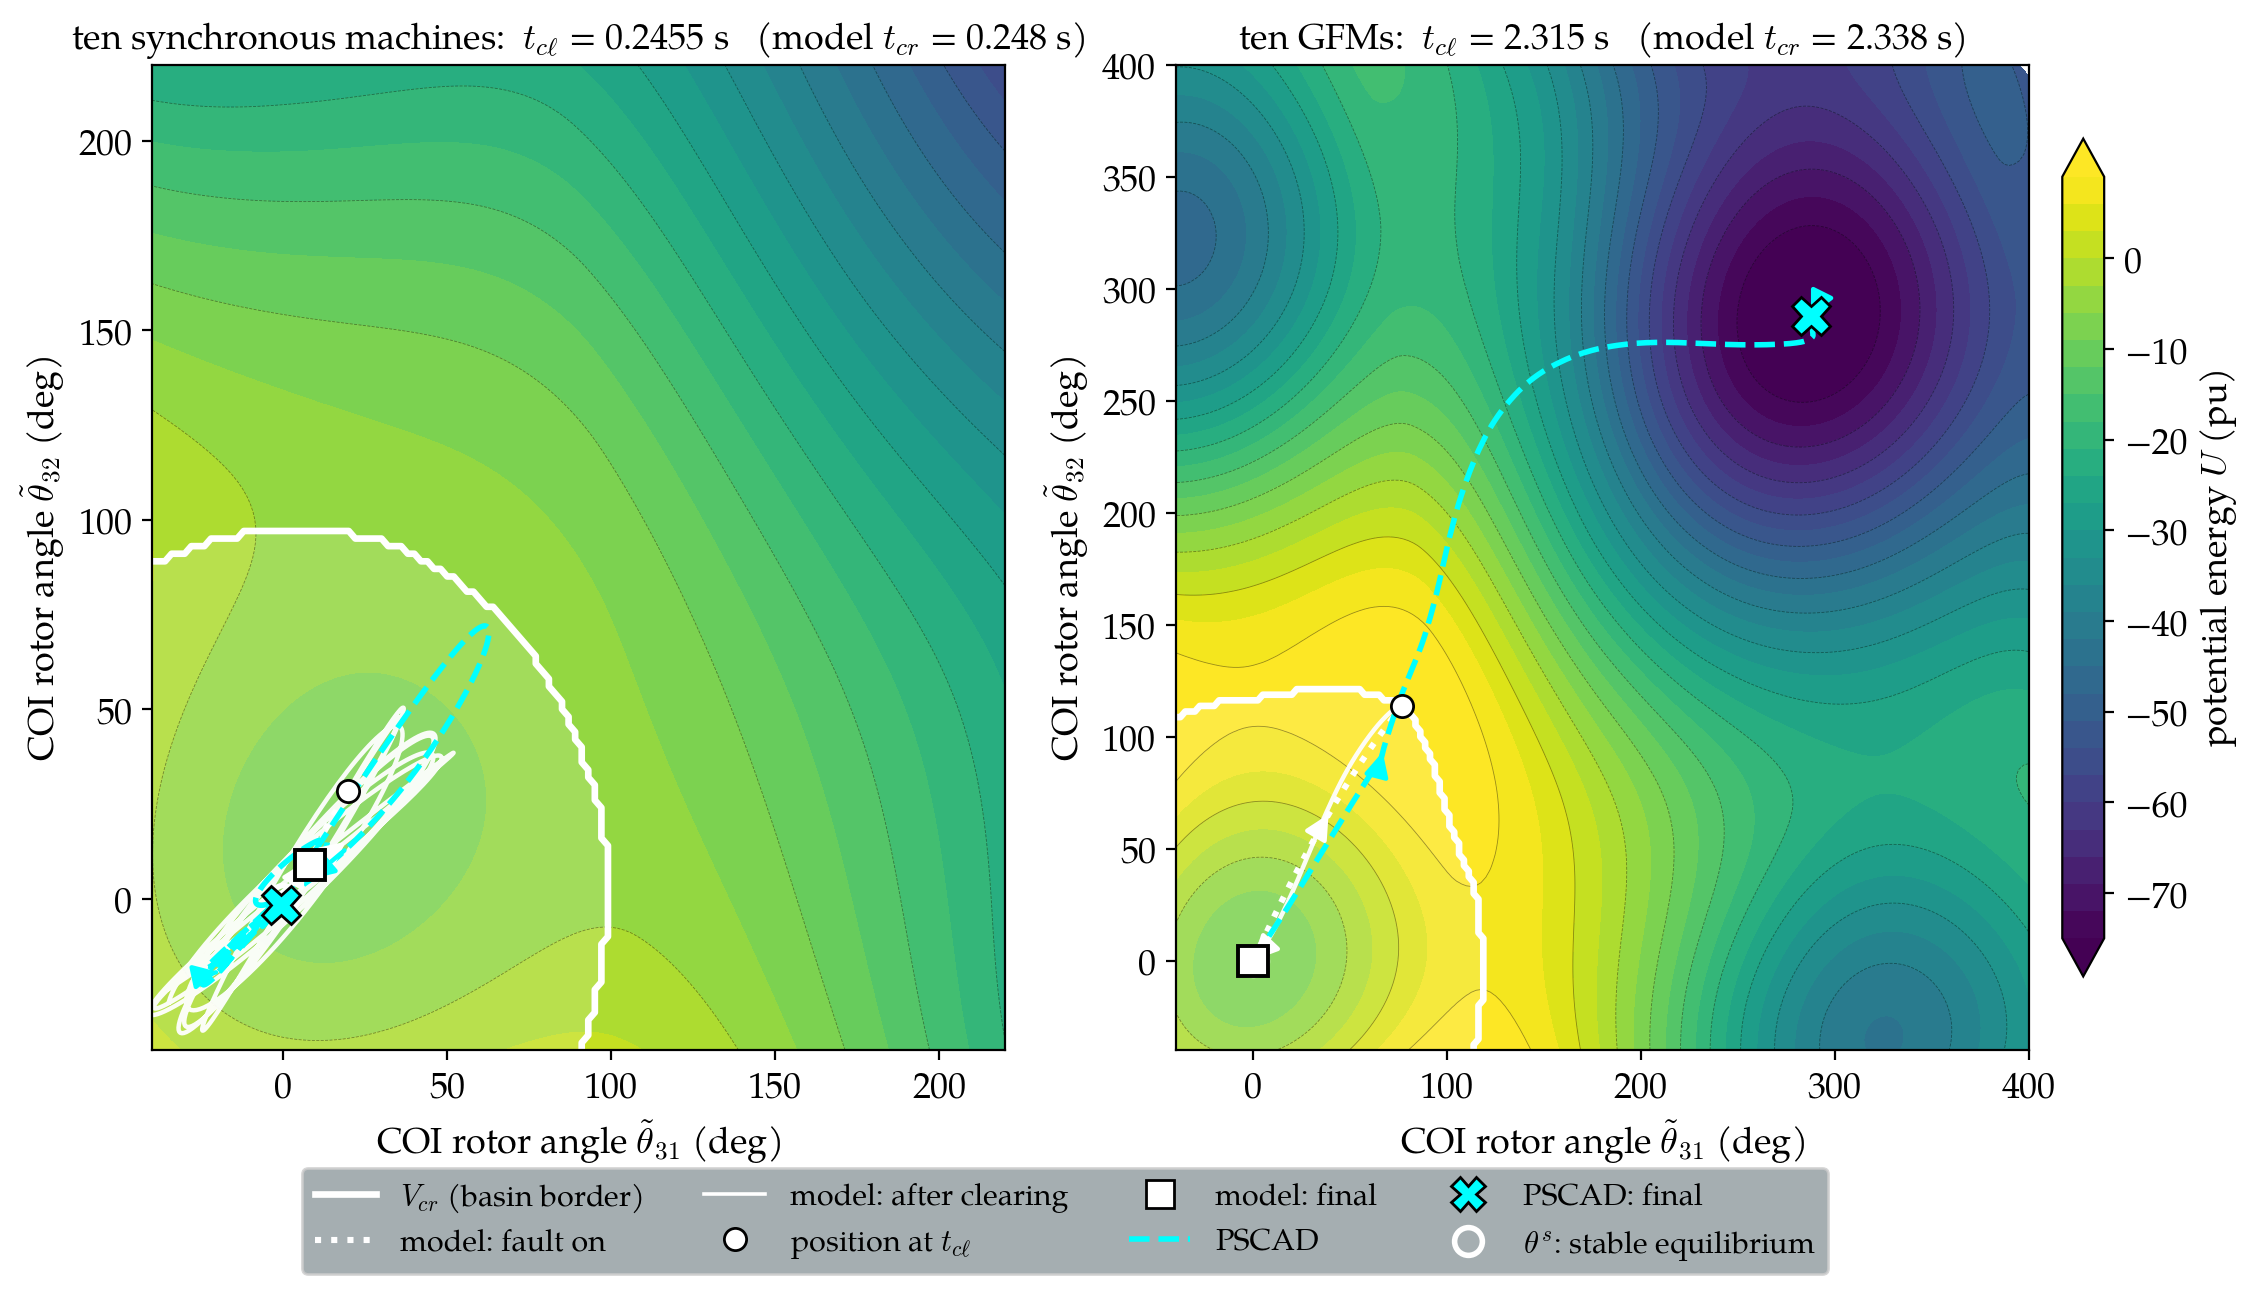
\includegraphics[width=\linewidth]{prism-uploads/at_model_cct_surface_meeting.png}}{0.2455}{2.315}
\par\vspace{4pt}
\energysurface{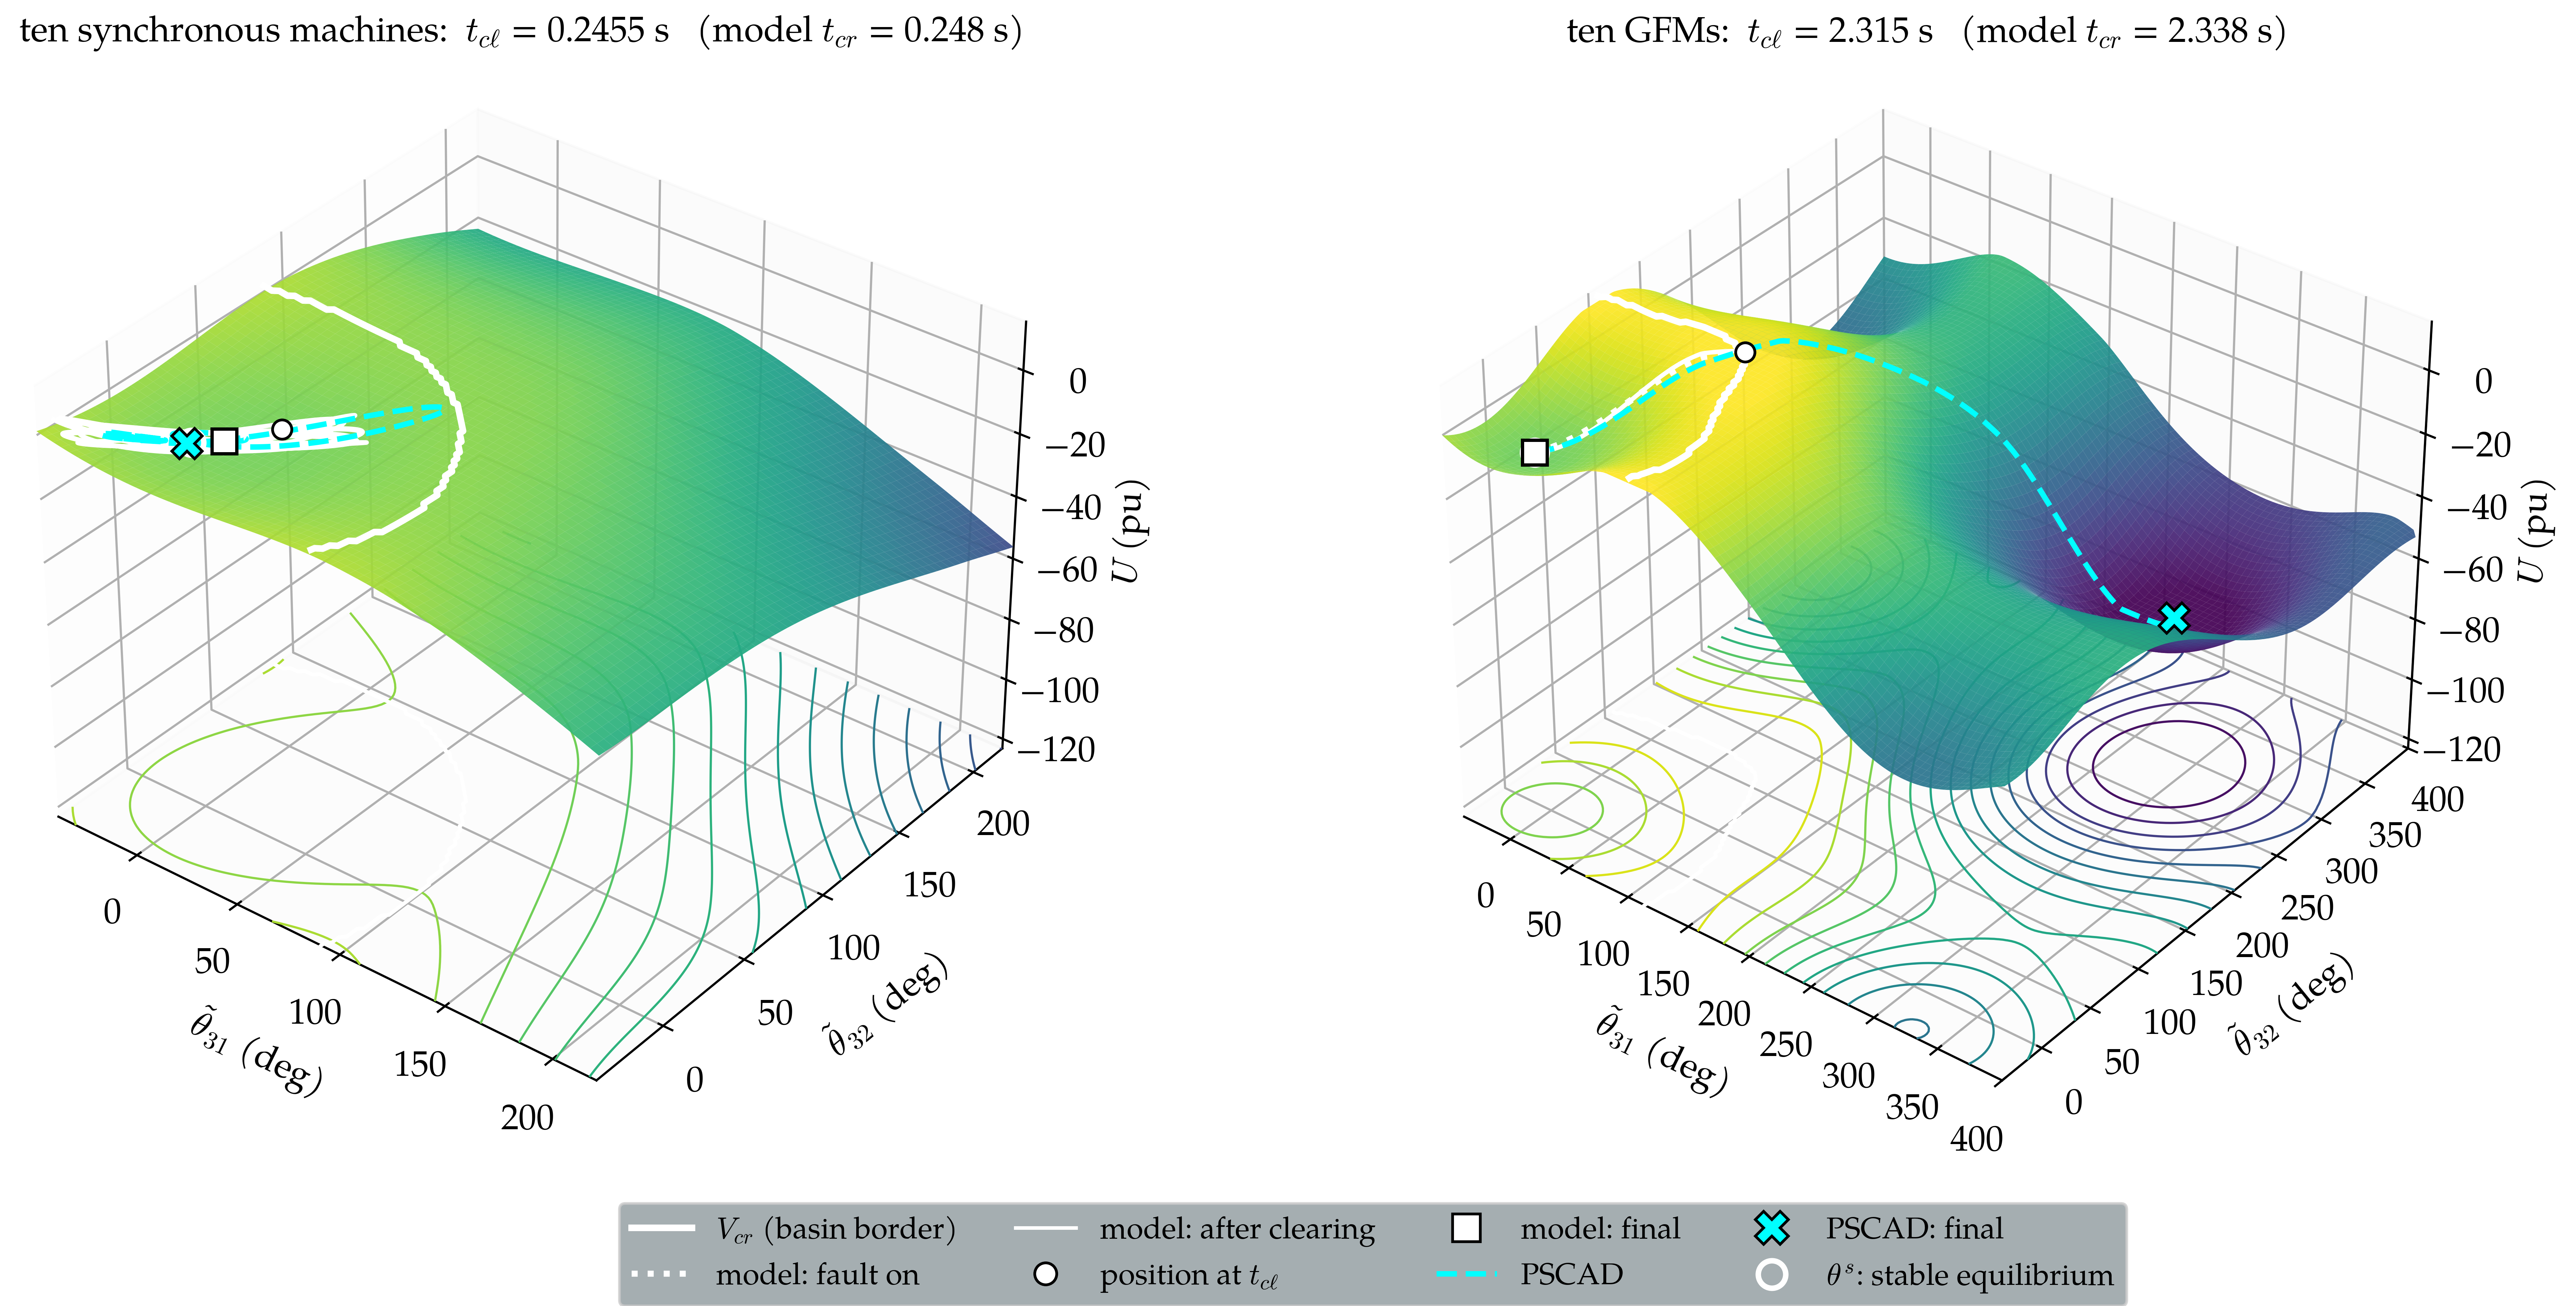
\includegraphics[width=\linewidth,trim=0 42.768bp 0 0,clip]{prism-uploads/at_model_cct_surface3d_meeting.png}}
\caption{Complementary views near the analytical critical clearing times: (a,b)~2D potential-energy contours and (c,d)~3D surfaces, synchronous machines on the left and GFM inverters on the right, in the equilibrium-shifted COI angles of Equation~\eqref{eq:energycoi} with the shared legend above the 3D views. Clearing durations are 0.2455~s and 2.315~s; model estimates are 0.248~s and 2.338~s. The GFM EMT endpoint lies in a neighboring well, unlike the model endpoint near the origin.}
\label{fig:esat}
\end{figure}

Current limiting and the ceiling on commanded voltage are plausible contributors to this discrepancy. When these constraints become active, the realized electrical power need not follow the sinusoidal relationship used by the classical construction. Figure~\ref{fig:satblock} illustrates how saturation changes the power-angle characteristic and the associated unstable equilibrium. Future controlled studies will isolate these effects rather than assume that omitted limiters explain every difference. The issue is the applicability of the chosen model assumptions, not a violation of classical stability theory. Figure~\ref{fig:ilimitsweep} shows the measured single-inverter clearing-time bracket as the transient current limit is raised from 2.0 to 15 per unit with all other settings fixed: the bracket rises from $(0.925,0.931]$~s at 2.0 per unit to $(1.163,1.169]$~s at 12 per unit and is unchanged at 15 per unit, where the limit exceeds the unlimited fault-current demand.

\begin{figure}[tbp]\centering
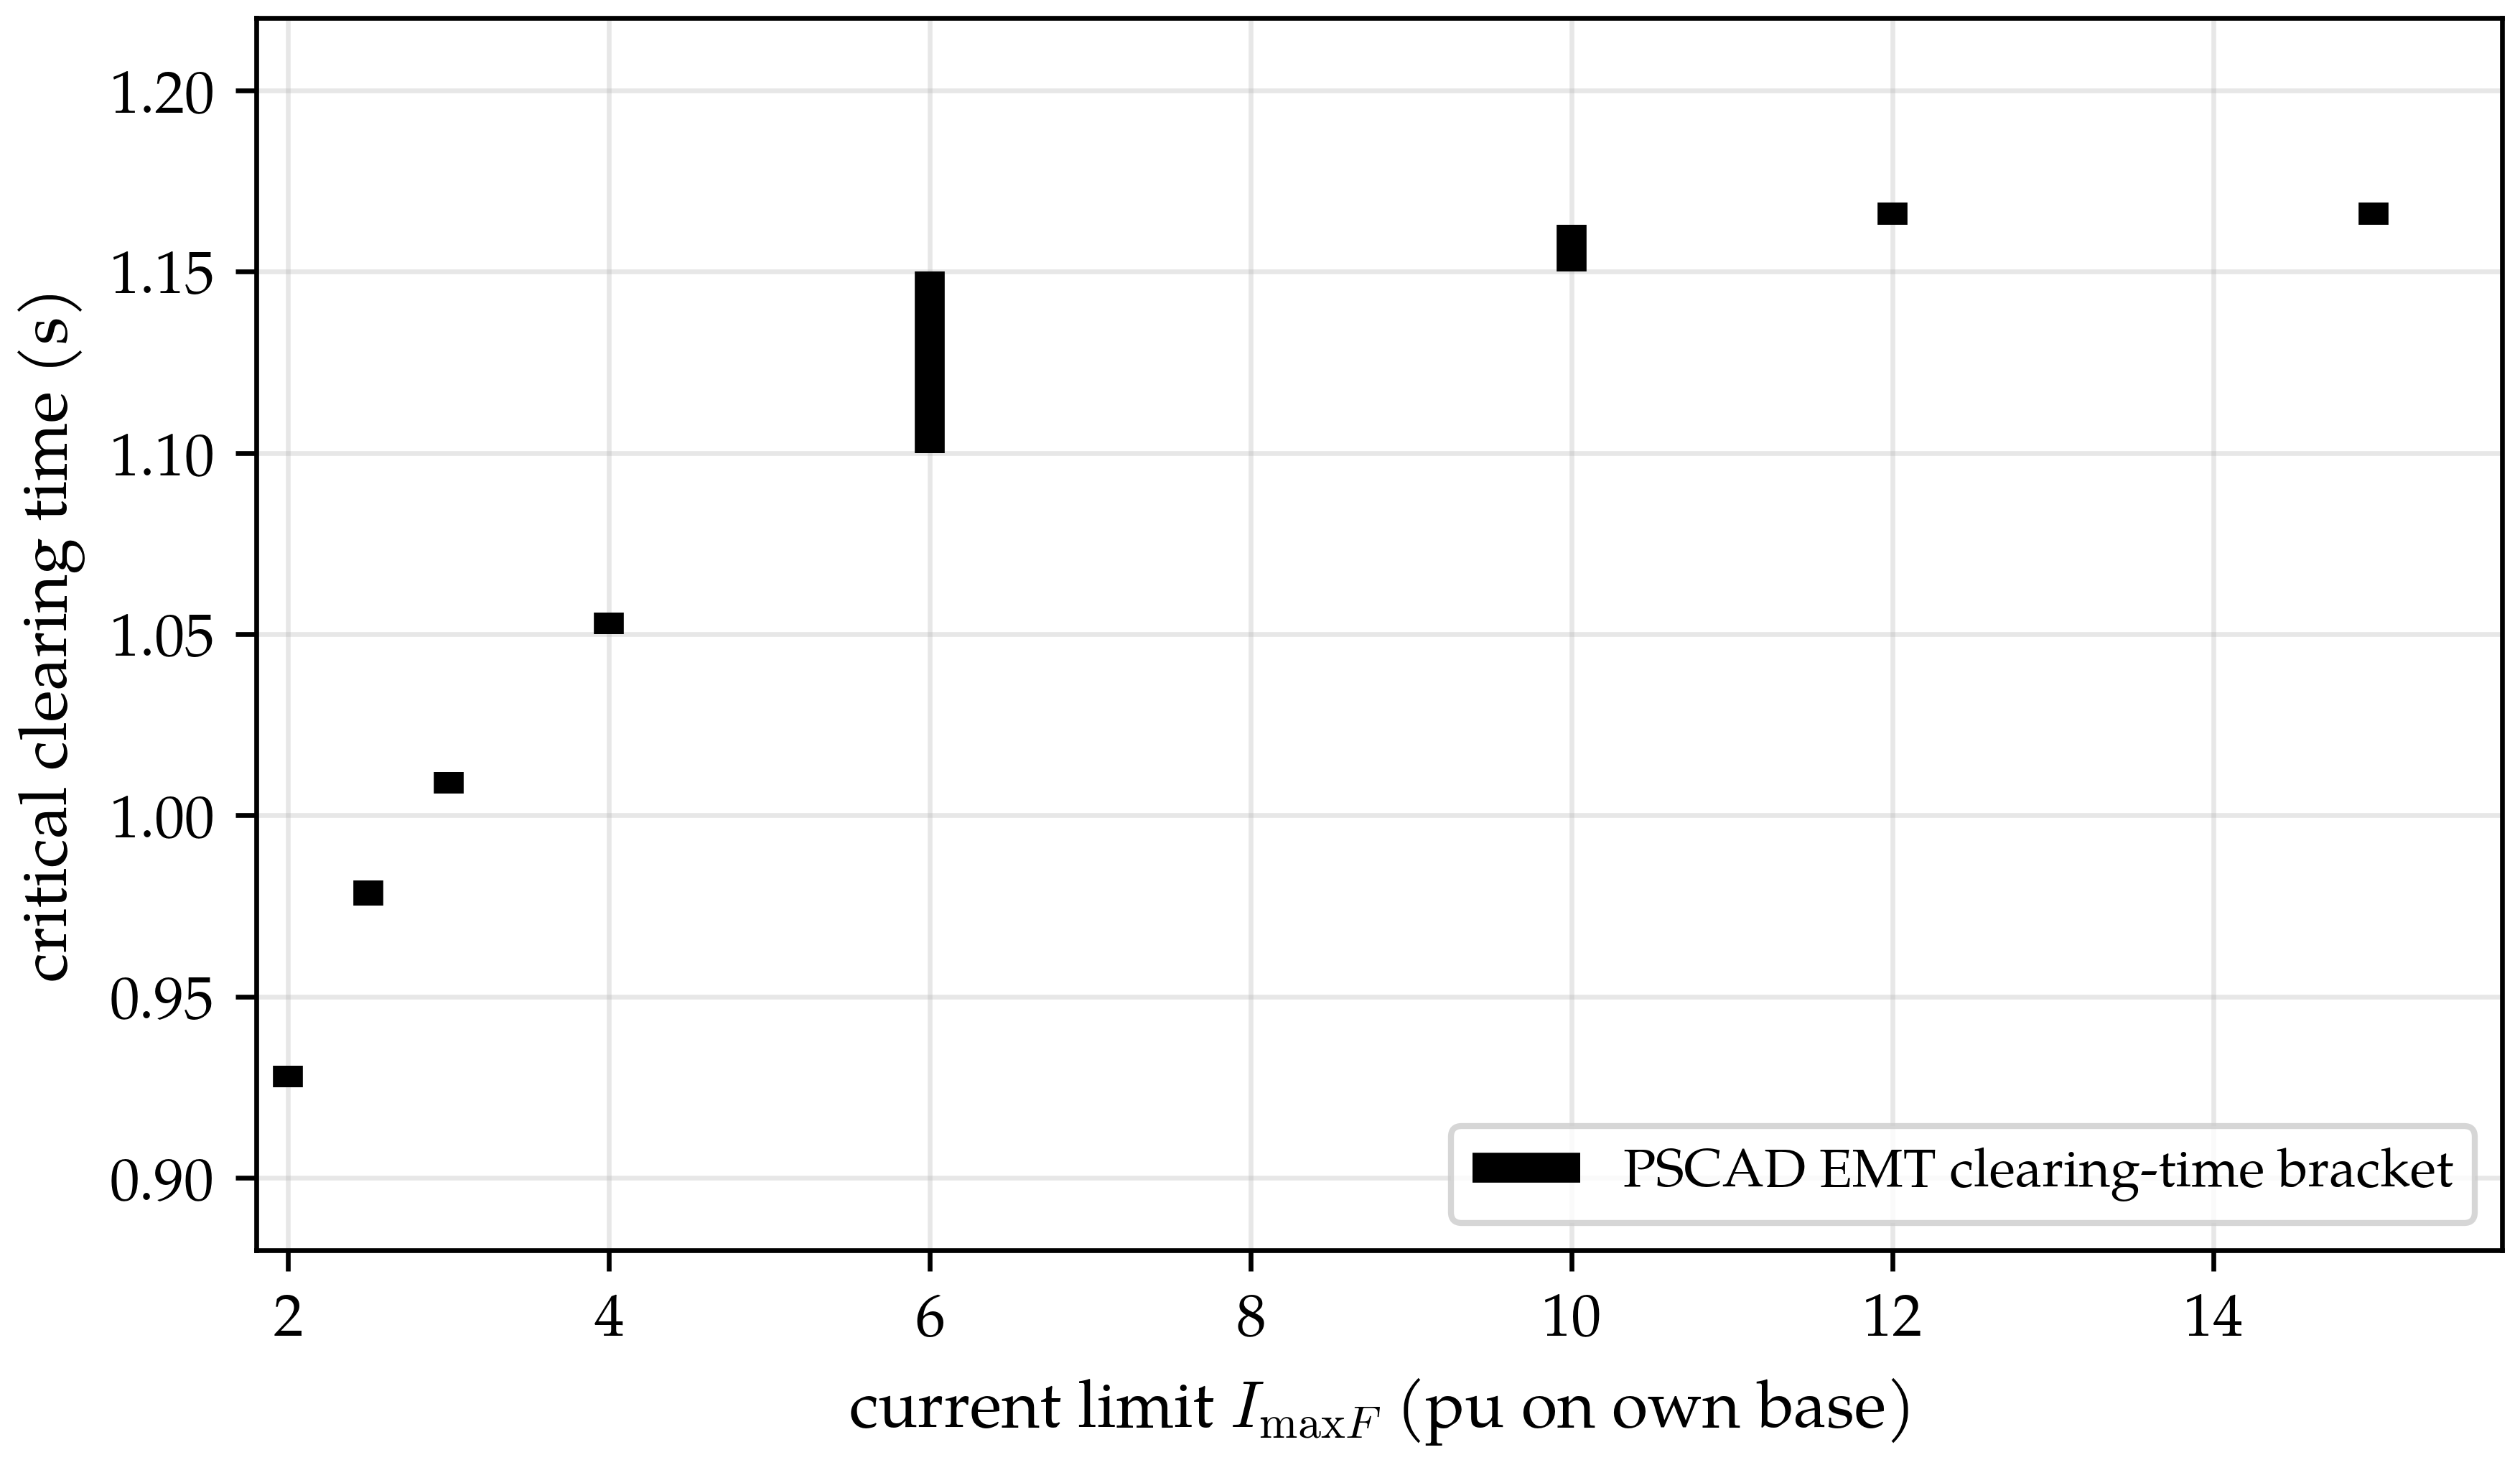
\includegraphics[width=0.9\textwidth]{ilimit_sweep_emt}
\caption{Measured critical clearing time of the single inverter on the infinite bus versus the transient current limit $I_{\max F}$, all other settings fixed; each bar is the bracket between the longest stable and the shortest unstable fault duration.}
\label{fig:ilimitsweep}
\end{figure}

\begin{figure}[tbp]\centering
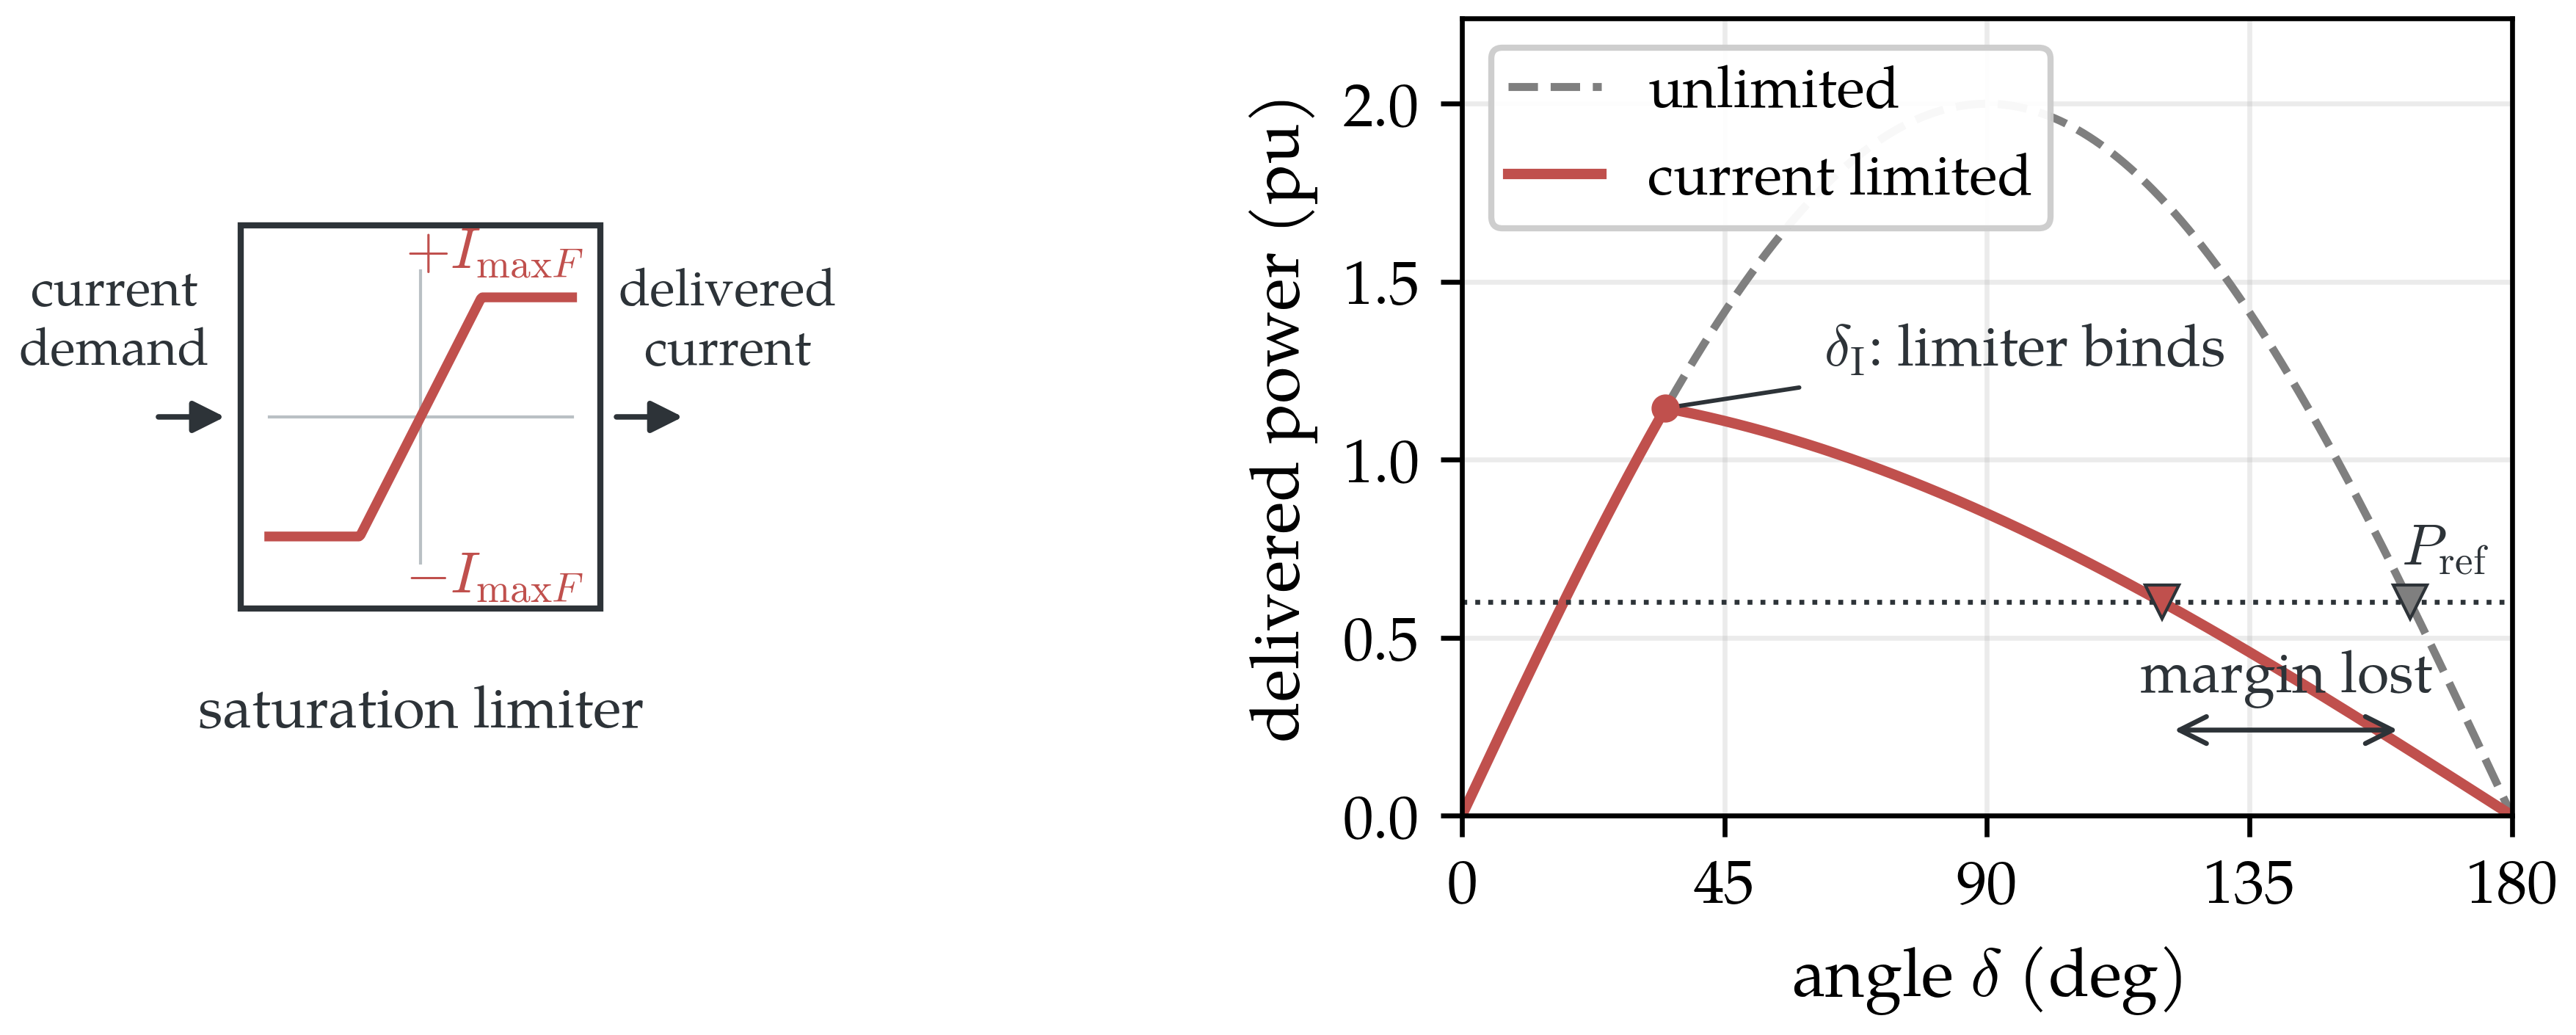
\includegraphics[width=0.9\textwidth]{saturation_block}
\caption{Conceptual effect of current saturation on the power-angle characteristic: the limited characteristic departs from the sinusoid, changing the unstable equilibrium and the region of attraction of the classical construction.}
\label{fig:satblock}
\end{figure}

\subsubsection{Modeling Goals}
\label{sec:nextsteps}
The next analytical steps build on this preliminary comparison. We will connect the model extensions to the same disturbances used in the testbed. Hardware studies remain a future direction after the simulation comparisons establish appropriate test cases.
\begin{itemize}
\item \textbf{Limiter-aware stability estimates.} Develop a critical-clearing-time analytical model for single and multi-inverter systems to include saturation and determine conditions under which the estimate is conservative.
\item \textbf{Guidance for manufacturers and operators.} Identify control parameters with the greatest influence on system-level stability for the configurations studied.
\item \textbf{Mixed-generation systems.} Extend the analysis to combinations of synchronous machines, GFM inverters of various control approaches, and GFL inverters.
\item \textbf{Additional disturbances.} Evaluate the models under unbalanced faults at other locations, faults with nonzero impedance, phase-angle jumps, and load steps.
\item \textbf{Large electronic loads.} Integrate large electronic load profiles and evaluate their effect on the fault ride-through capability of a system with a high share of grid-forming inverters.
\item \textbf{Hardware validation.} Investigate single-inverter infinite-bus and hardware-in-the-loop tests, followed by multi-inverter disturbances in the UT Austin laboratory microgrid.
\end{itemize}

\subsection{Conclusion}
\label{sec:conclusion}
We developed a reusable PSCAD EMT testbed for studying networks with increasing numbers of GFM resources. Starting from an IEEE 39-bus PSS/E case, we used E-TRAN to construct the network and equipped it with representative machine dynamics and selected inverter models. The first-year studies show fault ride through across the tested replacement configurations and useful differences between machine and GFM responses. The selected droop controls provide strong equivalent damping and low equivalent inertia, which help interpret the faster settling observed in the simulations.

The inertia-estimation and preliminary energy-method investigations connect those observations to familiar power-system concepts. They also show why damping contributions and active constraints matter when interpreting reduced models. The next phase will establish corresponding positive-sequence and EMT comparisons and examine how control, network, and load dynamics affect stability conclusions. The testbed provides a strong foundation for that work and for developing practical guidance on inverter-dominated power systems.

\section*{Acknowledgments}
\addcontentsline{toc}{section}{Acknowledgments}
This work was performed as part of the research collaboration between The University of Texas at Austin and the Electric Reliability Council of Texas (ERCOT). The authors gratefully acknowledge the technical discussions and support provided by members of the ERCOT and UNIFI communities.

\appendix
\section{Synchronous Machine Model Parameters}
\label{app:params}
The synchronous baseline combines GENROU, ESST4B, GGOV1, and PSS2B with an inertia constant of 5.46~s. The ten machines use the same ERCOT-supplied dynamic parameter set, while their ratings and operating points can differ. The bus-30 PSS/E record lists the parameters in standard model order:

\begin{lstlisting}[language={}]
30, 'GENROU', 1,
 7.61, 0.04, 0.98, 0.06, 5.46, 0, 1.99, 1.81,
 0.26, 0.45, 0.2, 0.15, 0.06, 0.32, //
30, 'ESST4B', 1,
 0, 4.0, 4.0, 1, -0.90, 0.01, 1, 0, 1, -0.90,
 0, 5.5, 0, 6.0, 0.1, 0, 0, //
30, 'GGOV1', 1,
 1, 1, 0.05, 1., 0.055, -0.055, 10, 1, 0, 1, 1,
 0.16, 0.5, 1.5, 0.2, 0.1, 0, 0, 3, 2, 0.7, 1,
 0, 0.1, -0.1, 0, 0.1, 10, 0.1, 0, 0.0002, 4, 5, 99, -99, //
30, 'PSS2B', 1,
 1, 0, 3, 0, 5, 1, 2, 2, 0, 2, 0, 2, 0.25, 1,
 0.5, 0.1, 15, 0.2, 0.031, 0.1, 0.02, 0, 0, 99, -99,
 99, -99, 0.1, -0.1, //
\end{lstlisting}

GENROU field~5 specifies the inertia constant $H=5.46$~s. For the REGFM\_A1 reference configuration, $m_{\mathrm{p}}=0.01$ and $T_{\mathrm{Pf}}=10$~ms give $H_{\mathrm{eq}}=0.5$~s and $D_{\mathrm{eq}}=100$ through Equation~\eqref{eq:heqdeq}. The replacement sizing uses $S_{\mathrm{inv,base}}=P_{\mathrm{G}}/0.6$, where $P_{\mathrm{G}}$ is generator dispatch in MW and the resulting base is in MVA. The bus-14 reference fault is bolted three-phase-to-ground for five cycles without reclosing; its 2.0 per-unit current limit is distinct from the 1.5 per-unit bus-10 study.

\section{PSCAD Output Files}
\label{app:plotting}
PSCAD writes numerical channels and channel descriptions to separate files. The processing workflow reconstructs them into a common table for analysis and plotting. This appendix describes that workflow, while the report also uses circuit diagrams, screenshots, and analytical illustrations.

\subsection{What PSCAD Writes}
For a project named \texttt{name}, EMTDC writes channel descriptions to \texttt{name.inf}. Numerical files follow the sequence \texttt{name\_01.out}, \texttt{name\_02.out}, and so on. Each output file contains simulation time followed by up to ten channels. The \texttt{PGB(...)} records in the \texttt{.inf} file provide channel indices and \texttt{Desc="..."} descriptions. The numerical files themselves do not name their columns.

\subsection{Channel Naming}
The harness parses the channel descriptions and converts them into column names. Repeated descriptions receive a suffix to keep the names unique. The following function illustrates this naming step:

\begin{lstlisting}
def inf_channel_names():
    names = []
    for line in open(project + ".inf"):
        if line.startswith("PGB("):
            names.append(line.split('Desc="')[1].split('"')[0]
                         .replace(":", "_"))
    seen, out = {}, []
    for n in names:                      # disambiguate duplicates
        seen[n] = seen.get(n, 0) + 1
        out.append(n if seen[n] == 1 else "%s_dup%d" % (n, seen[n]))
    return out
\end{lstlisting}

\subsection{Stitching and Export}
The exporter combines the output-file family using \texttt{OutFile} from the PSCAD file utilities. It checks modification times against the run start to avoid reading a previous run's output and compares the column count with the channel descriptions. It then downsamples the table and selects the declared channels for export:

\begin{lstlisting}
fout = OutFile(project_stem)             # name_01.out, name_02.out, ...
fout.toCSV(csv="_res_full.csv")          # stitched: TIME + all channels
df = pd.read_csv("_res_full.csv")
names = inf_channel_names()
if len(df.columns) != len(names) + 1:    # TIME + channels, exactly
    raise RuntimeError("column mismatch vs .inf")
df.columns = ["TIME"] + names
df = df.loc[::DOWNSAMPLE, ["TIME"] + KEEP]
df.to_csv(run_dir + "/rung_%s.csv" % tag, index=False)
\end{lstlisting}

Each run produces a CSV identified by its fault duration. This organization supports comparison of successful and unsuccessful runs when constructing clearing-time brackets. The channel names accompany the numerical values so that subsequent analysis can identify each recorded signal.

\subsection{Plotting Conventions}
Time-domain plots mark the fault interval and use a pre-fault window to establish the baseline. Network plots show RMS bus voltages in kV, currents in kA, and powers in MW and MVAr; device comparisons use per unit on each device base, stated in the caption. Two current measurements appear: the generator-bus channels are taken on the 230~kV side of each unit's step-up transformer, and a GFM unit's internal current magnitude is the inverter's own measurement at its terminals on the 10~kV side, in per unit of the unit rating; each caption states which is shown. Axes identify units, and multi-device panels share limits where appropriate. Ratings, dispatch, and terminal measurement locations remain important when comparing devices; per-unit presentation alone does not make the cases identical.

\begin{thebibliography}{99}
\setlength{\itemsep}{2pt}
\raggedright
\bibitem{chatterjee2026note} D.~Chatterjee, \emph{Inertia Estimation
for GFM Inverters}, internal technical note, June~24, 2026
(unpublished).
\bibitem{esrint2026} ERCOT Grid Operations, \emph{ESR Integration
Report}, August 2, 2026.
\bibitem{gis2026} ERCOT, \emph{Generator Interconnection Status
Report}, July 2026 (published August 3, 2026).
\bibitem{mohammadi2026} S.~Mohammadi, W.~Wang, M.~C.~I. Wada,
R.~Haghighi, A.~Hassan, H.~Liu, A.~Bhatnagar, A.~Chen, and W.~Su,
``Grid integration of AI data centers: a critical review of energy
storage solutions,'' \emph{Advances in Applied Energy}, 2026.
\url{https://www.sciencedirect.com/science/article/pii/S2666792426000302}
(preprint: \url{https://arxiv.org/abs/2603.00415})
\bibitem{unifi2026} UNIFI Consortium, \emph{UNIFI Specifications for
GFM Inverter-Based Resources, Version~3},
Rep.~UNIFI-2026-2-1 (also NLR/TP-5D00-98381), January 2026.
\url{https://docs.nlr.gov/docs/fy26osti/98381.pdf}
\bibitem{nogrr272} ERCOT, \emph{NOGRR272: Advanced Grid Support Requirements for Inverter-Based ESRs}, approved November~6, 2025; effective December~1, 2025. Official issue record and approval documents. \url{https://www.ercot.com/mktrules/issues/NOGRR272}
\bibitem{mora2026} ERCOT, \emph{Monthly Outlook for Resource Adequacy
(MORA)}, July 2026.
\url{https://www.ercot.com/files/docs/2026/05/01/MORA_July2026.pdf}
\bibitem{pscad39bus} Manitoba Hydro International, ``IEEE 39 bus
system,'' PSCAD Knowledge Base, Article~28.
\url{https://www.pscad.com/knowledge-base/article/28}
\bibitem{pscad39note} Manitoba Hydro International, \emph{IEEE 39 Bus
System Technical Note}.
\url{https://www.pscad.com/knowledge-base/download/ieee_39_bus_technical_note.pdf}
\bibitem{du2023a1} W.~Du et al., \emph{Model Specification of
Droop-Controlled, GFM Inverters (REGFM\_A1)}, Pacific
Northwest National Laboratory, Richland, WA, Rep.~PNNL-35110,
September 2023. \url{https://www.pnnl.gov/main/publications/external/technical_reports/PNNL-35110.pdf}
\bibitem{pnnlgithub} W.~Du, \emph{PSCAD and PSSE Version of WECC
Grid-Forming Inverter Models} (software release~V1, includes
REGFM\_A1, REGFM\_B1, REGFM\_C1, and REPCGFM\_C1), Pacific Northwest National
Laboratory, May 20, 2026.
\url{https://github.com/pnnl/PSCAD-and-PSSE-Version-of-WECC-Grid-Forming-Inverter-Models/releases/tag/V1}
\bibitem{ut26xrepo} N.~Roe, \emph{ERCOT--UT Austin Grid-Forming Inverter Testbed: report source, PSCAD test systems, run data, and processing scripts}, GitHub repository, The University of Texas at Austin, 2026.
\url{https://github.com/nroe413/ERCOT_project_finalReport_26X}
\bibitem{du2024b1} W.~Du et al., \emph{Virtual Synchronous Machine
GFM Inverter Model Specification (REGFM\_B1)}, UNIFI
Consortium, Rep.~UNIFI-2024-6-1, 2024.
\url{https://www.osti.gov/biblio/2376832}
\bibitem{pmview} ERCOT, ``PMView: model-quality test harness for
PSCAD.'' \url{https://sites.google.com/view/pmview/home}
\bibitem{dwg24} ERCOT Dynamics Working Group, \emph{Procedure Manual},
Revision~24, June~2025. \url{https://www.ercot.com/committees/ros/dwg}
\bibitem{pypscad} National Laboratory of the Rockies (NLR),
``PyPSCAD: Kenyon GFM inverter library.''
\url{https://github.com/NatLabRockies/PyPSCAD}
\bibitem{pscadgfm} Manitoba Hydro International, ``GFM
inverter model,'' PSCAD Knowledge Base, Article~894.
\url{https://www.pscad.com/knowledge-base/article/894}
\bibitem{huang2019} L.~Huang, H.~Xin, Z.~Wang, L.~Zhang, K.~Wu, and
J.~Hu, ``Transient stability analysis and control design of
droop-controlled voltage source converters considering current
limitation,'' \emph{IEEE Trans. Smart Grid}, vol.~10, no.~1,
pp.~578--591, 2019.
\bibitem{chatterjee2025eac} D.~Chatterjee, B.~Johnson, and G.-S. Seo,
``Is equal area criterion applicable for transient stability assessment
of GFM inverters?,'' in \emph{Proc. IEEE PES General Meeting},
2025, doi:10.1109/PESGM52009.2025.11225302.
\bibitem{chatterjee2025compel} D.~Chatterjee, N.~Baeckeland,
B.~Johnson, G.-S. Seo, and S.~Dhople, ``Demystifying GFM
inverter large-signal stability assessment with equivalent-circuit
models,'' in \emph{Proc. IEEE COMPEL}, 2025,
doi:10.1109/COMPEL57166.2025.11121209.
\bibitem{chatterjee2025ecce} D.~Chatterjee, B.~Yang, B.~Johnson, and
G.-S. Seo, ``Interaction energy-based transient stability framework for
multi-GFM inverter systems,'' in \emph{Proc. IEEE ECCE}, 2025,
doi:10.1109/ECCE58356.2025.11260189.
\bibitem{sauer1998} P.~W. Sauer and M.~A. Pai, \emph{Power System
Dynamics and Stability}. Upper Saddle River, NJ: Prentice Hall, 1998
(Ch.~9: energy-function methods).
\bibitem{kundur1994} P.~Kundur, \emph{Power System Stability and
Control}. New York: McGraw-Hill, 1994.
\bibitem{demello1969} F.~P. deMello and C.~Concordia, ``Concepts of synchronous machine stability as affected by excitation control,'' \emph{IEEE Trans. Power App. Syst.}, vol.~PAS-88, no.~4, pp.~316--329, Apr. 1969, doi:10.1109/TPAS.1969.292452.
\bibitem{ieee2800} IEEE Standards Association, \emph{IEEE Standard for
Interconnection and Interoperability of Inverter-Based Resources (IBRs)
Interconnecting with Associated Transmission Electric Power Systems},
IEEE Std 2800-2022, 2022 (Annex~K.2.2).
\bibitem{pai1989} M.~A. Pai, \emph{Energy Function Analysis for Power
System Stability}. Boston, MA: Kluwer Academic Publishers, 1989.
\bibitem{athay1979} T.~Athay, R.~Podmore, and S.~Virmani, ``A practical
method for the direct analysis of transient stability,'' \emph{IEEE
Trans. Power Apparatus and Systems}, vol.~PAS-98, no.~2, pp.~573--584,
1979.
\bibitem{bergen1981} A.~R. Bergen and D.~J. Hill, ``A structure
preserving model for power system stability analysis,'' \emph{IEEE
Trans. Power Apparatus and Systems}, vol.~PAS-100, no.~1, pp.~25--35,
1981.
\bibitem{chiang1988} H.-D. Chiang, F.~F. Wu, and P.~P. Varaiya,
``Foundations of the potential energy boundary surface method for power
system transient stability analysis,'' \emph{IEEE Trans. Circuits and
Systems}, vol.~35, no.~6, pp.~712--728, 1988.
\bibitem{popov1961} V.~M. Popov, ``Absolute stability of nonlinear
systems of automatic control,'' \emph{Automation and Remote Control},
vol.~22, no.~8, pp.~857--875, 1961.
\bibitem{zames1966} G.~Zames, ``On the input--output stability of
time-varying nonlinear feedback systems, Parts I and II,''
\emph{IEEE Trans. Automatic Control}, vol.~11, no.~2--3, 1966.
\bibitem{khalil2002} H.~K. Khalil, \emph{Nonlinear Systems}, 3rd~ed.
Upper Saddle River, NJ: Prentice Hall, 2002.
\bibitem{ags2026} S.-H. Huang (ERCOT), \emph{NPRRxxx Advanced Grid
Support Incentive Program Concept Overview}, ERCOT Inverter-Based
Resource Working Group, March 27, 2026.
\url{https://www.ercot.com/files/docs/2026/03/27/AGS-Incentive-Program-Concept-Overview-IBRWG-03272026.pdf}

\bibitem{etran} Electranix Corporation, \emph{E-TRAN: PSS/E to PSCAD Translation Software}. \url{https://www.electranix.com/software/}
\bibitem{pscadbergeron} Manitoba Hydro International, ``The Bergeron Model,'' in \emph{EMTDC User's Guide: Transmission Lines}, PSCAD online help. \url{https://www.pscad.com/webhelp/EMTDC/Transmission_Lines/The_Bergeron_Model.htm}
\bibitem{etranlib} Electranix Corporation, \emph{E-TRAN Runtime Library for PSCAD}. \url{https://www.electranix.com/software/e-tran-runtime-library-for-pscad/}
\bibitem{regfma1lib} Pacific Northwest National Laboratory, \emph{REGFM\_A1 PSCAD model release (REGFM\_A1.zip, containing PNNL\_REGFM\_A1\_gf46.lib)}, GitHub release V1 of \emph{PSCAD and PSSE Version of WECC Grid-Forming Inverter Models}. \url{https://github.com/pnnl/PSCAD-and-PSSE-Version-of-WECC-Grid-Forming-Inverter-Models/releases/download/V1/REGFM_A1.zip}
\bibitem{iannuzzo2014} F.~Iannuzzo, C.~Abbate, and G.~Busatto, ``Instabilities in silicon power devices: A review of failure mechanisms in modern power devices,'' \emph{IEEE Industrial Electronics Magazine}, vol.~8, no.~3, pp.~28--39, Sept. 2014, doi: 10.1109/MIE.2014.2305758.
\bibitem{agsupdate2026} ERCOT, \emph{Interconnection and Grid Analysis Update}, Item~9, April~2026, advanced grid-support implementation update. \url{https://www.ercot.com/files/docs/2026/04/13/9-Interconnection-and-Grid-Analysis-Update.pdf}
\bibitem{pestr1} IEEE Power \& Energy Society, Task Force on Turbine-Governor Modeling, \emph{Dynamic Models for Turbine-Governors in Power System Studies}, Technical Report PES-TR1, January 2013, Appendix~C (GGOV1 typical parameters). \url{https://site.ieee.org/fw-pes/files/2013/01/PES_TR1.pdf}
\bibitem{pssemodels} Siemens Industry, Inc., \emph{PSS\textsuperscript{\textregistered}E Model Library}, GGOV1 (GE general governor/turbine model), ICONs Rselect and Flag followed by the 33 CONs R through R\textsubscript{down}.
\bibitem{nerc2017scr} North American Electric Reliability Corporation, \emph{Integrating Inverter-Based Resources into Low Short Circuit Strength Systems}, Reliability Guideline, December 2017, Ch.~1, ``Short Circuit Ratio (SCR).'' \url{https://www.nerc.com/globalassets/who-we-are/standing-committees/rstc/irpwg/item_4a._integrating-_inverter-based_resources_into_low_short_circuit_strength_systems_-_2017-11-08-final.pdf}
\bibitem{rao2011} S.~S. Rao, \emph{Mechanical Vibrations}, 5th~ed. Upper Saddle River, NJ: Prentice Hall, 2011, Sec.~2.6.3, ``Logarithmic Decrement.''
\end{thebibliography}

\end{document}

